% 高一45_交附闵行_国庆作业2.tex
%   —— 高一上数学“2026-2027 年交附闵行高一上国庆作业 2”（试卷版/答案版）
% 试卷版：xelatex 高一45_交附闵行_国庆作业2.tex
% 答案版：xelatex "\def\isanswer{1}% 高一45_交附闵行_国庆作业2.tex
%   —— 高一上数学“2026-2027 年交附闵行高一上国庆作业 2”（试卷版/答案版）
% 试卷版：xelatex 高一45_交附闵行_国庆作业2.tex
% 答案版：xelatex "\def\isanswer{1}% 高一45_交附闵行_国庆作业2.tex
%   —— 高一上数学“2026-2027 年交附闵行高一上国庆作业 2”（试卷版/答案版）
% 试卷版：xelatex 高一45_交附闵行_国庆作业2.tex
% 答案版：xelatex "\def\isanswer{1}% 高一45_交附闵行_国庆作业2.tex
%   —— 高一上数学“2026-2027 年交附闵行高一上国庆作业 2”（试卷版/答案版）
% 试卷版：xelatex 高一45_交附闵行_国庆作业2.tex
% 答案版：xelatex "\def\isanswer{1}\input{高一45_交附闵行_国庆作业2.tex}"
% 紧凑版：xelatex "\def\iscompact{1}\input{高一45_交附闵行_国庆作业2.tex}"
%
% 原始材料是微信公众号图文（公众号“魔都数学加油站”，作者“破晓”，2026-10-02 17:56 发布，
% 连载“27学年高一45”，原文标题“27学年高一45——2026-2027年上海市交附闵行高一上国庆作业2”，
% https://mp.weixin.qq.com/s/1xdCtzH-3Il0jJrz3saiPA），正文为 10 张 PNG 页。
% 第 01—06、09 页为 4762×6735；第 07、08、10 页为 2560×3620（同一篇各页原图分辨率不一致）。
% 原文本身是一份讲评版：第 3—21 题均照原卷保留题目与题下解析；第 13 题原卷把答案 C 印在括号中。
% 题目、选项、答案与解析均照原卷录入，未改内容；卷面的粉色斜水印及页脚不录入。
%
% 卷首标题：原卷印作“2026-2027 年交附闵行高一上国庆作业 2”（公众号标题里的“上海市”
% 三字卷面标题行没有，本稿照卷面），年份区间按全稿惯例排 en dash，前缀照原卷保留“年”。
%
% 与原卷的排版差异：
%   ① 原卷印有“一、填空题”“二、选择题”“三、解答题”三节标题，本稿照原卷分节，
%      只把标题改排成全稿统一的“大节标题”样式；
%   ② 第 13 题原卷在题干括号内直接印答案 C，本稿按全稿样式将括号留空、答案移入答案版的 \ans{}；
%   ③ 原卷填空横线及选择题答案括号均按全稿样式排版，填空横线统一用 \blankline[4.4em]；
%   ④ 原卷第 20 题配有十字形广场示意图，本稿在源码中用 TikZ 重绘，图中区域、边界及点名照原卷。
%   ⑤ 原卷未印副标题，本稿按本卷实际涉及的知识模块补出“集合与常用逻辑用语、不等式”。
%
% 原卷存疑/错误（均照抄原卷、未改，见对应题目处上方注释）：
%   ① 第 11 题解析原卷印"所以 p=3+9=12，又 12,15∉A，所以 12,15∉B"，与 A∪\overline{B} 的条件
%      及后文 B 的根为 6、9 均一致，无矛盾，本稿照录（早前记录的"∈B／前后矛盾"系本稿误读）；
%   ② 第 15 题题干与解析均按原卷印 ac<0，解析"因为 a<b<c，且 ac<0，所以 a<0，c>0"与题设一致，
%      无矛盾（早前记录的"abc<0／解析冲突"系本稿误读题干所致）；本稿照录原卷答案与解析。
%   ③ 第 20 题原卷各数（造价 2100 元/m^2、W_1=2100x^2、合并式 2000x^2+200000/x^2+19000、
%      末句 59000 元）经复核自洽，无矛盾（早前记录的"W_1=200x^2／末句 5900 元"系本稿误录）；本稿照录。
%   ④ 第 18(2) 题 a=-1 时 A=B=(-1,1)，不满足“B 是 A 的真子集”，故原解析给出的 a≤-1 应为 a<-1；
%   ⑤ 第 19(2) 题原卷用"{c|0<c<1}∩{c|c<-2√3/3 或 c>2√3/3}=∅"论证"不等式①、②中至多有一个恒成立"，
%      论证成立（早前记录的"区间并集留有间隙"系本稿误录解析所致）；本稿照录原卷。
%
\documentclass[a4paper,11pt]{article}
\usepackage{common}

\begin{document}

\examtitlest[3]{2026--2027 年交附闵行高一上国庆作业 2}{集合与常用逻辑用语、不等式}

\bigsec{一、填空题}

\begin{enumerate}
\setcounter{enumi}{2}

\item 满足 $A\cup\{-1,1\}=\{-1,0,1\}$ 的集合 $A$ 共有 \blankline[4.4em] 个.

\ifanswer
\solbegin
\step{集合可能为 $\{0\}$、$\{0,1\}$、$\{0,-1\}$、$\{0,1,-1\}$，共有 $4$ 个.}
\solend

\fi

\item 设 $x\in\R$，则“$x+\dfrac1x>2$”是“$x\neq1$”的 \blankline[4.4em] 条件.

\ifanswer
\solbegin
\step{$x+\dfrac1x>2\Longleftrightarrow x>0$ 且 $x\neq1$，故为充分不必要条件.}
\solend

\fi

\item 已知集合 $A=\{x\mid|x-1|<a\}$，$B=\{-4,3\}$，若 $A\cap B=\varnothing$，则 $a$ 的最大值为 \blankline[4.4em].

\ifanswer
\solbegin
\step{$A=\{x\mid -a<x-1<a\}=\{x\mid1-a<x<1+a\}$，$B=\{-4,3\}$，且 $A\cap B=\varnothing$，}
\step{$A=\varnothing$ 时，$1-a\geqslant1+a$，解得 $a\leqslant0$，满足 $A\cap B=\varnothing$；}
\step{若 $-4\in A$，则 $1-a<-4<1+a$，解得 $a>5$；}
\step{若 $3\in A$，则 $1-a<3<1+a$，解得 $a>2$，}
\step{因为 $A\cap B=\varnothing$，所以 $-4\notin A$ 且 $3\notin A$，所以 $a\leqslant5$ 且 $a\leqslant2$，所以 $a\leqslant2$，}
\step{综上，$a$ 的最大值为 $2$.}
\solend

\fi

\item 设 $x\in\R$，方程 $|x-1|+|2x-1|=|3x-2|$ 的解集为 \blankline[4.4em].

\ifanswer
\solbegin
\step{因为 $|x-1|+|2x-1|\geqslant|(x-1)+(2x-1)|=|3x-2|$，}
\step{当且仅当 $(x-1)(2x-1)\geqslant0$，解得 $x\leqslant\dfrac12$ 或 $x\geqslant1$，}
\step{故方程 $|x-1|+|2x-1|=|3x-2|$ 的解集为 $\left(-\infty,\dfrac12\right]\cup[1,+\infty)$.}
\solend

\fi

\item 已知 $a$、$b\in\R$，且 $3a+2b=1$，则 $8^a+4^b$ 最小值为 \blankline[4.4em].

\ifanswer
\solbegin
% 注：原卷本行与上行均作“$8^a+4^b$ 最小值为”，“最小值”前无“的”，原卷如此，照录未改。
\step{因为 $3a+2b=1$，所以 $8^a+4^b=2^{3a}+2^{2b}\geqslant2\sqrt{2^{3a+2b}}=2\sqrt2$，}
\step{当且仅当 $3a=2b$ 时取等号，故 $8^a+4^b$ 最小值为 $2\sqrt2$.}
\solend

\fi

\item 已知 $a>0$，$b>0$，且 $a+2b+ab=30$，则 $2a+b$ 的最小值为 \blankline[4.4em].

\ifanswer
\solbegin
\step{由 $a+2b+ab=30$，得 $(a+2)(b+1)=32$.}
\step{因为 $a>0$，$b>0$，所以 $a+2>0$，$b+1>0$，}
\step{所以 $2a+b=2(a+2)+(b+1)-5\geqslant2\sqrt{2\times32}-5=11$，}
\step{当且仅当 $2(a+2)=(b+1)$，即 $a=2$，$b=7$ 时取等号，}
\step{所以 $2a+b$ 的最小值为 $11$.}
\solend

\fi

\item 已知 $A=\{x\mid x^2+px+1=0\}$，$M=\{x\mid x>0\}$，若 $A\cap M=\varnothing$，则实数 $p$ 的取值范围为 \blankline[4.4em].

\ifanswer
\solbegin
\step{①当 $A=\varnothing$ 时，$\Delta=p^2-4<0$，所以 $-2<p<2$，此时满足 $A\cap M=\varnothing$；}
\step{②当 $A\neq\varnothing$ 时，$\Delta=p^2-4\geqslant0$，$p\geqslant2$ 或 $p\leqslant-2$，}
\step{因为 $M=\{x\mid x>0\}$，$A\cap M=\varnothing$，由韦达定理得 $\begin{cases}-p\leqslant0\\1>0\end{cases}$，解得 $p\geqslant0$，}
\step{所以 $p\geqslant2$，}
\step{由①②综合得 $p>-2$，故实数 $p$ 的取值范围为 $(-2,+\infty)$.}
\solend

\fi

\item 已知集合 $A=[t,t+1]\cup[t+3,t+6]$，其中 $t>0$. 若存在正数 $\lambda$，使得对任意 $a\in A$，都有 $\dfrac{\lambda}{a}\in A$，则 $t$ 的取值集合为 \blankline[4.4em].

\ifanswer
\solbegin
\step{因为 $0\notin A$，$t>0$，所以 $a\in[t,t+1]\cup[t+3,t+6]$，}
\step{则 $\dfrac1a\in\left[\dfrac1{t+6},\dfrac1{t+3}\right]\cup\left[\dfrac1{t+1},\dfrac1t\right]$，}
\step{又因为 $\lambda>0$，所以 $\dfrac{\lambda}{a}\in\left[\dfrac{\lambda}{t+6},\dfrac{\lambda}{t+3}\right]\cup\left[\dfrac{\lambda}{t+1},\dfrac{\lambda}{t}\right]$，}
\step{因为 $\dfrac{\lambda}{a}\in A$，所以 $\begin{cases}\dfrac{\lambda}{t+6}\geqslant t\\[3pt]\dfrac{\lambda}{t+3}\leqslant t+1\end{cases}$ 且 $\begin{cases}\dfrac{\lambda}{t+1}\geqslant t+3\\[3pt]\dfrac{\lambda}{t}\leqslant t+6\end{cases}$，}
% 注：原卷本行两个不等式组印作“$t(t+6)\leqslant\lambda\leqslant t(t+6)$”与
%     “$(t+1)(t+3)\leqslant\lambda\leqslant(t+1)(t+3)$”（两侧同式），与上行两式推导不合，系原卷笔误；
%     原卷如此，照录未改。
\step{得 $\begin{cases}t(t+6)\leqslant\lambda\leqslant t(t+6)\\[3pt](t+1)(t+3)\leqslant\lambda\leqslant(t+1)(t+3)\end{cases}$，所以 $\lambda=t(t+6)=(t+1)(t+3)$，}
\step{解得 $t=\dfrac32$，取值集合为 $\left\{\dfrac32\right\}$.}
\solend

\fi

\item 已知全集 $U=\{x\mid x=3n,1\leqslant n\leqslant5\ \text{且}\ n\in\N\}$，$A=\{x\mid x^2-px+27=0,p\in\N\}$，
$B=\{x\mid x^2-15x+q=0,q\in\N\}$，且 $A\cup\overline{B}=\{3,9,12,15\}$，则 $p+q$ 的值为 \blankline[4.4em].

\ifanswer
\solbegin
\step{因为全集 $U=\{3,6,9,12,15\}$，$A\cup\overline{B}=\{3,9,12,15\}$，}
\step{所以 $3$、$9$、$12$、$15$ 中可能有两个属于 $A$，}
\step{因为 $A$ 中的方程 $x^2-px+27=0$ 中，两根之积 $x_1x_2=27$，所以 $3$、$9\in A$，}
\step{所以 $p=3+9=12$，又 $12$、$15\notin A$，所以 $12$、$15\notin B$，}
\step{因为 $B$ 中的方程 $x^2-15x+q=0$ 中，两根之和 $x_3+x_4=15$，所以 $6$、$9\in B$，}
\step{则 $q=6\times9=54$，所以 $p+q=66$.}
\solend

\fi

\item 若关于 $x$ 的不等式 $|x-2k|+|x-3k|<4k$ 共有 $2025$ 个整数解，则实数 $k$ 的取值范围为 \blankline[4.4em].

\ifanswer
\solbegin
\step{显然 $k>0$，由 $|x-2k|+|x-3k|<4k$，得 $\dfrac{k}{2}<x<\dfrac{9k}{2}$，}
\step{因为该不等式共有 $2025$ 个整数解，所以 $2024<\dfrac{9k}{2}-\dfrac{k}{2}\leqslant2026$，}
\step{解得 $506<k\leqslant506.5$，}
\step{由 $\dfrac{k}{2}\in(253,253.25]$，得这 $2025$ 个整数解只能为 $254,255,256,\cdots,2278$，}
\step{所以 $2278<\dfrac{9k}{2}\leqslant2279$，解得 $506\dfrac29<k\leqslant506\dfrac49$，结合 $506<k\leqslant506.5$，}
\step{得 $k$ 的取值范围是 $\left(506\dfrac29,506\dfrac49\right]$.}
\solend

\fi

\end{enumerate}

\bigsec{二、选择题}

\begin{enumerate}
\setcounter{enumi}{12}

\item 已知 $a,b\in\R$，且 $ab\neq0$，则下列结论恒成立的是\mbox{（\quad）}

\keepwithprev
A. $a+b\geqslant2\sqrt{ab}$\qquad
B. $\left(\dfrac{a+b}{2}\right)^2>ab$\qquad
C. $\left|\dfrac ab+\dfrac ba\right|\geqslant2$\qquad
D. $a^2+b^2>2ab$

\ans{$C$}

\item 如果 $a^{2025}+b^{2025}=0$，那么一定有\mbox{（\quad）}

\keepwithprev
A. $(|a|+|b|)^{2025}=0$\qquad
B. $(a-b)^{2025}=0$\qquad
C. $(a\cdot b)^{2025}=0$\qquad
D. $(a+b)^{2025}=0$

\ans{$D$}

\ifanswer
\solbegin
\step{由 $a^{2025}+b^{2025}=0$，得 $a^{2025}=-b^{2025}=(-b)^{2025}$，则 $\left(a^{2025}\right)^{\frac{1}{2025}}=\left[(-b)^{2025}\right]^{\frac{1}{2025}}$，}
\step{即 $a=-b$，即 $a+b=0$，故 $(a+b)^{2025}=0$，故 D 符合题意；}
\step{对于 A，若取 $a=1$，$b=-1$，则 $(|a|+|b|)^{2025}=2^{2025}\neq0$，故 A 不合题意；}
\step{对于 B，若取 $a=1$，$b=-1$，则 $(a-b)^{2025}=2^{2025}\neq0$，故 B 不合题意；}
\step{对于 C，若取 $a=1$，$b=-1$，则 $(a\cdot b)^{2025}=(-1)^{2025}=-1\neq0$，故 C 不合题意；}
\step{故选 D.}
\solend

\fi

\item 已知 $a$、$b$、$c$ 满足 $a<b<c$，且 $ac<0$，那么下列各式中一定成立的是\mbox{（\quad）}

\keepwithprev
A. $\dfrac1a>\dfrac1c$\qquad
B. $ab^2<cb^2$\qquad
C. $ac<bc$\qquad
D. $a+c>2b$

\ans{$C$}

\ifanswer
\solbegin
\step{因为 $a<b<c$，且 $ac<0$，所以 $a<0$，$c>0$，}
\step{对于 A，$\dfrac1a<0<\dfrac1c$，故 A 错误；}
\step{对于 B，当 $b=0$ 时，$ab^2=cb^2$，故 B 错误；}
\step{对于 C，$ac<bc$ 可化为 $(a-b)c<0$，因为 $a<b$，所以 $a-b<0$，}
\step{又因为 $c>0$，所以 $(a-b)c<0$，所以 C 正确；}
\step{对于 D，设 $a=-2$，$b=0$，$c=1$，则 $a+c<2b$，故 D 错误.}
\step{故选 C.}
\solend

\fi

\item 对于 $a\in\R$，设集合 $A=\left\{x\mid\dfrac{(x^2-6x+a)(x-1)}{x+a}=0\right\}$，记 $A$ 的所有元素之和为 $S(a)$，
所有元素之积为 $T(a)$，则下列说法中，正确的是\mbox{（\quad）}

\keepwithprev
A. 不存在实数 $a$，使得 $S(a)=6$\qquad
B. 存在实数 $a$，使得 $T(a)=9$

C. 存在无数实数 $a$，使得 $S(a)=7$\qquad
D. 若 $T(a)=3$，则 $a=3$

\ans{$C$}

\ifanswer
\solbegin
\step{要使 $\dfrac{(x^2-6x+a)(x-1)}{x+a}=0$，只需 $(x^2-6x+a)(x-1)=0$ 且 $x+a\neq0$，}
\step{由 $(x^2-6x+a)(x-1)=0$ 得 $x^2-6x+a=0$ 或 $x-1=0$，}
\step{对于一元二次方程 $x^2-6x+a=0$，其判别式 $\Delta=36-4a$，}
\step{当 $\Delta=0$，即 $a=9$ 时，集合 $A=\{1,3\}$，$S(a)=4$，$T(a)=3$；}
\step{当 $\Delta<0$，即 $a>9$ 时，集合 $A=\{1\}$，$S(a)=T(a)=1$；}
\step{当 $\Delta>0$，即 $a<9$ 时，一元二次方程 $x^2-6x+a=0$ 的解为 $x=3\pm\sqrt{9-a}$，}
\step{①当 $a=0$ 时，$x\neq0$，则集合 $A=\{1,6\}$，则 $S(a)=7$，$T(a)=6$，}
\step{②当 $a=-7$ 时，$x\neq7$，则集合 $A=\{-1,1\}$，则 $S(a)=0$，$T(a)=-1$，}
% 注：下一行集合 A 原卷印作 {-1,1}（按 a=-1 代入 x^2-6x-1=0 应得 3±√10，原卷如此，照录未改）。
\step{③当 $a=-1$ 时，$x\neq1$，则集合 $A=\{-1,1\}$，则 $S(a)=6$，$T(a)=-1$，}
\step{④当 $a=5$ 时，$x\neq-5$，则集合 $A=\{1,5\}$，则 $S(a)=6$，$T(a)=5$，}
\step{⑤当 $a\neq5,0,-1,-7$ 时，集合 $A=\{1,3-\sqrt{9-a},3+\sqrt{9-a}\}$，}
\step{则 $S(a)=7$，$T(a)=a$.}
\step{选项 A，当 $a=5$ 时，$S(a)=6$，所以 A 错误；}
\step{选项 B，$T(a)$ 的可能值为 $-1,1,3,5,6,a$（$a<9$），无 $T(a)=9$，所以 B 错误；}
\step{选项 C，当 $a<9$，且 $a\neq5,-1,-7$ 时，$S(a)=7$，有无数个 $a$ 满足，所以 C 正确；}
\step{选项 D，当 $T(a)=3$ 时，有 $a=3$ 和 $a=9$ 满足，所以 D 错误.}
\step{故选 C.}
\solend

\fi

\end{enumerate}

\bigsec{三、解答题}

\begin{enumerate}
\setcounter{enumi}{16}

\item 已知 $a\in\R$，关于 $x$ 的不等式 $|x+1|+|x-1|>a^2-5a+4$.

\begin{enumerate}[label=(\arabic*)]
\item 当 $a=0$ 时，求不等式的解集；
\item 若不等式的解集为 $\R$，求 $a$ 的取值范围.
\end{enumerate}

\ifanswer
\solbegin
\stepm{(1)}{当 $a=0$ 时，不等式为 $|x+1|+|x-1|>4$，}
\step{又 $|x+1|+|x-1|=\begin{cases}2x,&x\geqslant1\\2,&-1<x<1\\-2x,&x\leqslant-1\end{cases}$，}
\step{则 $|x+1|+|x-1|>4$ 的解为 $x>2$ 或 $x<-2$，}
\step{即不等式的解集为 $(-\infty,-2)\cup(2,+\infty)$；}
\stepm{(2)}{不等式 $|x+1|+|x-1|>a^2-5a+4$ 的解集为 $\R$，}
\step{则 $(|x+1|+|x-1|)_{\min}>a^2-5a+4$，}
\step{又 $(|x+1|+|x-1|)_{\min}=2$，当且仅当 $-1\leqslant x\leqslant1$ 时取得，即 $a^2-5a+4<2$，}
\step{即 $a^2-5a+2<0$，即 $\dfrac{5-\sqrt{17}}2<a<\dfrac{5+\sqrt{17}}2$，}
\step{即 $a$ 的取值范围为 $\left(\dfrac{5-\sqrt{17}}2,\dfrac{5+\sqrt{17}}2\right)$.}
\solend

\fi

\ansspace[6]

\item 已知集合 $A=\{x\mid(x-a)(x-a^2)<0\}$，集合 $B=\left\{x\mid\dfrac{2x}{x-1}<1\right\}$，命题 $p:x\in A$，命题 $q:x\in B$.

\begin{enumerate}[label=(\arabic*)]
\item 当实数 $a$ 为何值时，$A=B$；
\item 若 $q$ 是 $p$ 的充分不必要条件，求实数 $a$ 的取值范围.
\end{enumerate}

\ifanswer
\solbegin
\stepm{(1)}{由 $\dfrac{2x}{x-1}<1$ 得 $\dfrac{2x}{x-1}-1=\dfrac{x+1}{x-1}<0$，解得 $-1<x<1$，即 $B=\{x\mid-1<x<1\}$，}
\step{因为 $A=\{x\mid(x-a)(x-a^2)<0\}$，$A=B$，所以 $\begin{cases}a=-1\\a^2=1\end{cases}$，解得 $a=-1$；}
\stepm{(2)}{若 $q$ 是 $p$ 的充分不必要条件，则 $B\subset A$，}
\step{当 $a^2=a$，即 $a=0$ 或 $a=1$ 时，$A=\varnothing$，显然不符合题意；}
\step{当 $a^2>a$，即 $a>1$ 或 $a<0$ 时，$A=(a,a^2)$，则 $\begin{cases}a\leqslant-1\\a^2\geqslant1\\a>1\ \text{或}\ a<0\end{cases}$，}
% 注：a=-1 时 A=(-1,1)=B，不是 B 的真子集；原解析用 B⊂A 但答案含 -1，照录。
\step{前两等号不能同时取得，解得 $a\leqslant-1$；}
\step{当 $a^2<a$，即 $0<a<1$ 时，$A=(a^2,a)$，显然不符合题意，}
\step{故 $a$ 的范围为 $\{a\mid a\leqslant-1\}$.}
\solend

\fi

\ansspace[6]

\item 已知不等式① $x^2+2cx+c>0$，② $x^2+cx+c^2-1>0$，其中 $c$ 是实数.

\begin{enumerate}[label=(\arabic*)]
\item 若 $1$ 是不等式②的一个解，求实数 $c$ 的取值范围；
\item 证明：不等式①、②中至多有一个恒成立.
\end{enumerate}

\ifanswer
\solbegin
\stepm{(1)}{已知不等式① $x^2+2cx+c>0$，② $x^2+cx+c^2-1>0$，}
\step{又 $1$ 是不等式②的一个解，则 $1+c+c^2-1>0$，}
\step{则 $c^2+c>0$，则 $c<-1$ 或 $c>0$，则 $c$ 的取值范围为 $(-\infty,-1)\cup(0,+\infty)$；}
\stepm{(2)}{若不等式①恒成立，则 $\Delta=4c^2-4c<0$，则 $0<c<1$，}
\step{若不等式②恒成立，则 $\Delta=c^2-4(c^2-1)=4-3c^2<0$，}
\step{则 $c<-\dfrac{2\sqrt3}{3}$ 或 $c>\dfrac{2\sqrt3}{3}$，}
\step{又 $\{c\mid 0<c<1\}\cap\left\{c\mid c<-\dfrac{2\sqrt3}{3}\ \text{或}\ c>\dfrac{2\sqrt3}{3}\right\}=\varnothing$，}
\step{则不存在实数 $c$ 使得不等式①、②同时恒成立，}
\step{则不等式①、②中至多有一个恒成立.}
\solend

\fi

\ansspace[6]

\item 为践行“科技强国”战略，某社区计划建造一座融合智慧节能技术的八边形休闲广场，其中两个相同的矩形 $ABCD$ 和 $EFGH$ 构成的十字形区域总面积为 $200\text{m}^2$. 中心正方形 $MNPQ$ 区域将安装国产太阳能光伏板（兼具休憩遮阳功能），造价为 $2100$ 元$/\text{m}^2$；周围四个矩形区域（图中阴影部分）铺设透水地砖，造价为 $105$ 元$/\text{m}^2$；再在四个三角形区域种植耐旱固碳植物，助力碳中和，造价为 $40$ 元$/\text{m}^2$. 设总造价为 $W$（单位：元），$AD=x$（单位：m）.

\begin{center}
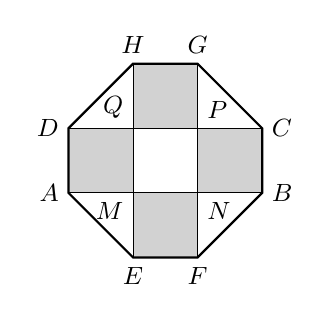
\begin{tikzpicture}[scale=0.82, every node/.style={font=\small}]
  \fill[gray!35] (-1.5,-0.5) rectangle (1.5,0.5);
  \fill[gray!35] (-0.5,-1.5) rectangle (0.5,1.5);
  % 中心正方形 MNPQ 原卷不涂阴影，照原卷留白：
  \fill[white] (-0.5,-0.5) rectangle (0.5,0.5);
  \draw[thick] (-1.5,0.5)--(-0.5,1.5)--(0.5,1.5)--(1.5,0.5)--(1.5,-0.5)--(0.5,-1.5)--(-0.5,-1.5)--(-1.5,-0.5)--cycle;
  \draw (-1.5,-0.5) rectangle (1.5,0.5);
  \draw (-0.5,-1.5) rectangle (0.5,1.5);
  \node[left] at (-1.5,0.5) {$D$};
  \node[left] at (-1.5,-0.5) {$A$};
  \node[right] at (1.5,0.5) {$C$};
  \node[right] at (1.5,-0.5) {$B$};
  \node[above] at (-0.5,1.5) {$H$};
  \node[above] at (0.5,1.5) {$G$};
  \node[below] at (-0.5,-1.5) {$E$};
  \node[below] at (0.5,-1.5) {$F$};
  \node[below left] at (-0.5,-0.5) {$M$};
  \node[below right] at (0.5,-0.5) {$N$};
  \node[above right] at (0.5,0.5) {$P$};
  \node[above left] at (-0.5,0.5) {$Q$};
\end{tikzpicture}
\end{center}

\begin{enumerate}[label=(\arabic*)]
\item 设 $DQ$ 长为 $y$（单位：m），用 $x$ 表示 $y$，并求出 $x$ 的取值范围；
\item $AD$ 取何值时可使总造价最低，并求出最低造价.
\end{enumerate}

\ifanswer
\solbegin
\stepm{(1)}{设 $AD=x\text{m}$（$x>0$），$DQ=y\text{m}$（$y>0$），}
\step{因为十字形区域总面积为 $200\text{m}^2$，所以 $4xy+x^2=200$，}
\step{解得 $y=\dfrac{200-x^2}{4x}=\dfrac{50}{x}-\dfrac{x}{4}$，}
\step{因为 $x>0$，$y>0$，所以 $y=\dfrac{200-x^2}{4x}>0$，解得 $0<x<10\sqrt2$，}
\step{所以 $y=\dfrac{50}{x}-\dfrac{x}{4}$，$0<x<10\sqrt2$；}
\stepm{(2)}{中心正方形 $MNPQ$ 区域，造价为 $2100$ 元$/\text{m}^2$，}
\step{中心正方形 $MNPQ$ 面积为 $S_1=x^2$，造价为 $W_1=2100\times S_1=2100x^2$；}
\step{周围四个矩形区域（图中阴影部分）铺设透水地砖，造价为 $105$ 元$/\text{m}^2$，}
\step{四个矩形的总面积为 $S_2=4xy=4x\left(\dfrac{50}{x}-\dfrac{x}{4}\right)=200-x^2$，}
\step{造价为 $W_2=105\times S_2=105(200-x^2)=21000-105x^2$；}
\step{四个三角形区域种植耐旱固碳植物，助力碳中和，造价为 $40$ 元$/\text{m}^2$，}
\step{四个三角形的总面积为 $S_3=4\times\dfrac12y^2=2\left(\dfrac{50}{x}-\dfrac{x}{4}\right)^2
=\dfrac{5000}{x^2}-50+\dfrac{x^2}{8}$，}
\step{造价为 $W_3=40\times S_3=40\left(\dfrac{5000}{x^2}-50+\dfrac{x^2}{8}\right)
=\dfrac{200000}{x^2}-2000+5x^2$；}
\step{设总造价为 $W$（单位：元），}
\step{则总造价为 $W=W_1+W_2+W_3$}
\step{$=2100x^2+21000-105x^2+\dfrac{200000}{x^2}-2000+5x^2$}
\step{$=2000x^2+\dfrac{200000}{x^2}+19000$，}
\step{又 $2000x^2+\dfrac{200000}{x^2}\geqslant2\sqrt{2000x^2\times\dfrac{200000}{x^2}}=2\times20000=40000$，}
\step{当且仅当 $2000x^2=\dfrac{200000}{x^2}$，即 $x=\sqrt{10}$（在 $x$ 的范围内）时取等号，}
\step{所以 $W=2000x^2+\dfrac{200000}{x^2}+19000\geqslant59000$，当 $x=\sqrt{10}$ 时取等号，}
\step{故当 $AD$ 的长为 $\sqrt{10}$ 时，总造价最低，为 $59000$ 元.}
\solend

\fi

\ansspace[8]

\item 对于实数 $a$、$b$、$c$，若 $|a-c|<|b-c|$，则称 $a$ 比 $b$ 更接近于 $c$. 现已知 $p$、$q$ 都是正有理数.

\begin{enumerate}[label=(\arabic*)]
\item 证明：$\sqrt3$ 必在 $\dfrac pq$ 和 $\dfrac{p+3q}{p+q}$ 之间；
\item 试问 $\dfrac pq$ 和 $\dfrac{p+3q}{p+q}$ 这两个数，哪一个更接近于 $\sqrt3$？说明你的理由；
\item 请你再写出一个有理数，使得它的值比 $\dfrac pq$ 和 $\dfrac{p+3q}{p+q}$ 的值更接近于 $\sqrt3$，并说明你的理由.
\end{enumerate}

\ifanswer
\solbegin
\stepm{(1)}{设 $a=\dfrac pq$（$a$ 为正有理数），则需证 $\sqrt3$ 在 $a$ 和 $\dfrac{a+3}{a+1}$（即 $\dfrac{p+3q}{p+q}$）之间.}
\step{当 $a>\sqrt3$ 时，计算 $a-\dfrac{a+3}{a+1}$ 得 $a-\dfrac{a+3}{a+1}=\dfrac{a(a+1)-(a+3)}{a+1}=\dfrac{a^2-3}{a+1}$，}
\step{$a>\sqrt3$，则 $a^2-3>0$，故 $a>\dfrac{a+3}{a+1}$；}
\step{再计算 $\dfrac{a+3}{a+1}-\sqrt3$ 得 $\dfrac{a+3}{a+1}-\sqrt3=\dfrac{(1-\sqrt3)(a-\sqrt3)}{a+1}$，}
\step{$1-\sqrt3<0$，$a-\sqrt3>0$，$a+1>0$，}
\step{故 $\dfrac{a+3}{a+1}-\sqrt3<0$，即 $\dfrac{a+3}{a+1}<\sqrt3$，从而 $\dfrac{a+3}{a+1}<\sqrt3<a$；}
\step{当 $a<\sqrt3$ 时，同理可得 $a<\dfrac{a+3}{a+1}$ 且 $\dfrac{a+3}{a+1}>\sqrt3$，即 $a<\sqrt3<\dfrac{a+3}{a+1}$，}
\step{综上，$\sqrt3$ 必在 $\dfrac pq$ 和 $\dfrac{p+3q}{p+q}$ 之间；}
\stepm{(2)}{设 $a=\dfrac pq$，$b=\dfrac{p+3q}{p+q}=\dfrac{a+3}{a+1}$，比较 $|a-\sqrt3|$ 与 $|b-\sqrt3|$，}
\step{由（1）得 $(a-\sqrt3)(b-\sqrt3)<0$，}
\step{$\dfrac{|b-\sqrt3|}{|a-\sqrt3|}
=\left|\dfrac{b-\sqrt3}{a-\sqrt3}\right|
=\dfrac{\left|\dfrac{(1-\sqrt3)(a-\sqrt3)}{a+1}\right|}{|a-\sqrt3|}
=\dfrac{\sqrt3-1}{a+1}$，}
\step{$a>0$，$a+1>1$，$\sqrt3-1<1$，故 $\dfrac{\sqrt3-1}{a+1}<1$，即 $|b-\sqrt3|<|a-\sqrt3|$，}
\step{即 $\dfrac{p+3q}{p+q}$ 比 $\dfrac pq$ 更接近于 $\sqrt3$；}
\stepm{(3)}{$\dfrac{2p+3q}{p+2q}$，理由：}
\step{设 $b=\dfrac{p+3q}{p+q}$，新数 $c=\dfrac{b+3}{b+1}=\dfrac{2p+3q}{p+2q}$，}
\step{由（1）得 $(b-\sqrt3)(c-\sqrt3)<0$，}
\step{$c-\sqrt3=\dfrac{b+3}{b+1}-\sqrt3=\dfrac{(1-\sqrt3)(b-\sqrt3)}{b+1}$，}
\step{则 $\dfrac{|c-\sqrt3|}{|b-\sqrt3|}
=\left|\dfrac{c-\sqrt3}{b-\sqrt3}\right|
=\dfrac{\left|\dfrac{(1-\sqrt3)(b-\sqrt3)}{b+1}\right|}{|b-\sqrt3|}
=\dfrac{\sqrt3-1}{b+1}$，}
\step{$b>0$，$b+1>1$，$0<\sqrt3-1<1$，故 $\dfrac{\sqrt3-1}{b+1}<1$，即 $|c-\sqrt3|<|b-\sqrt3|$，}
\step{即 $\dfrac{2p+3q}{p+2q}$ 比 $\dfrac{p+3q}{p+q}$ 更接近于 $\sqrt3$，故 $c$ 更接近 $\sqrt3$.}
\solend

\fi

\ansspace*[10]

\end{enumerate}

\end{document}
"
% 紧凑版：xelatex "\def\iscompact{1}% 高一45_交附闵行_国庆作业2.tex
%   —— 高一上数学“2026-2027 年交附闵行高一上国庆作业 2”（试卷版/答案版）
% 试卷版：xelatex 高一45_交附闵行_国庆作业2.tex
% 答案版：xelatex "\def\isanswer{1}\input{高一45_交附闵行_国庆作业2.tex}"
% 紧凑版：xelatex "\def\iscompact{1}\input{高一45_交附闵行_国庆作业2.tex}"
%
% 原始材料是微信公众号图文（公众号“魔都数学加油站”，作者“破晓”，2026-10-02 17:56 发布，
% 连载“27学年高一45”，原文标题“27学年高一45——2026-2027年上海市交附闵行高一上国庆作业2”，
% https://mp.weixin.qq.com/s/1xdCtzH-3Il0jJrz3saiPA），正文为 10 张 PNG 页。
% 第 01—06、09 页为 4762×6735；第 07、08、10 页为 2560×3620（同一篇各页原图分辨率不一致）。
% 原文本身是一份讲评版：第 3—21 题均照原卷保留题目与题下解析；第 13 题原卷把答案 C 印在括号中。
% 题目、选项、答案与解析均照原卷录入，未改内容；卷面的粉色斜水印及页脚不录入。
%
% 卷首标题：原卷印作“2026-2027 年交附闵行高一上国庆作业 2”（公众号标题里的“上海市”
% 三字卷面标题行没有，本稿照卷面），年份区间按全稿惯例排 en dash，前缀照原卷保留“年”。
%
% 与原卷的排版差异：
%   ① 原卷印有“一、填空题”“二、选择题”“三、解答题”三节标题，本稿照原卷分节，
%      只把标题改排成全稿统一的“大节标题”样式；
%   ② 第 13 题原卷在题干括号内直接印答案 C，本稿按全稿样式将括号留空、答案移入答案版的 \ans{}；
%   ③ 原卷填空横线及选择题答案括号均按全稿样式排版，填空横线统一用 \blankline[4.4em]；
%   ④ 原卷第 20 题配有十字形广场示意图，本稿在源码中用 TikZ 重绘，图中区域、边界及点名照原卷。
%   ⑤ 原卷未印副标题，本稿按本卷实际涉及的知识模块补出“集合与常用逻辑用语、不等式”。
%
% 原卷存疑/错误（均照抄原卷、未改，见对应题目处上方注释）：
%   ① 第 11 题解析原卷印"所以 p=3+9=12，又 12,15∉A，所以 12,15∉B"，与 A∪\overline{B} 的条件
%      及后文 B 的根为 6、9 均一致，无矛盾，本稿照录（早前记录的"∈B／前后矛盾"系本稿误读）；
%   ② 第 15 题题干与解析均按原卷印 ac<0，解析"因为 a<b<c，且 ac<0，所以 a<0，c>0"与题设一致，
%      无矛盾（早前记录的"abc<0／解析冲突"系本稿误读题干所致）；本稿照录原卷答案与解析。
%   ③ 第 20 题原卷各数（造价 2100 元/m^2、W_1=2100x^2、合并式 2000x^2+200000/x^2+19000、
%      末句 59000 元）经复核自洽，无矛盾（早前记录的"W_1=200x^2／末句 5900 元"系本稿误录）；本稿照录。
%   ④ 第 18(2) 题 a=-1 时 A=B=(-1,1)，不满足“B 是 A 的真子集”，故原解析给出的 a≤-1 应为 a<-1；
%   ⑤ 第 19(2) 题原卷用"{c|0<c<1}∩{c|c<-2√3/3 或 c>2√3/3}=∅"论证"不等式①、②中至多有一个恒成立"，
%      论证成立（早前记录的"区间并集留有间隙"系本稿误录解析所致）；本稿照录原卷。
%
\documentclass[a4paper,11pt]{article}
\usepackage{common}

\begin{document}

\examtitlest[3]{2026--2027 年交附闵行高一上国庆作业 2}{集合与常用逻辑用语、不等式}

\bigsec{一、填空题}

\begin{enumerate}
\setcounter{enumi}{2}

\item 满足 $A\cup\{-1,1\}=\{-1,0,1\}$ 的集合 $A$ 共有 \blankline[4.4em] 个.

\ifanswer
\solbegin
\step{集合可能为 $\{0\}$、$\{0,1\}$、$\{0,-1\}$、$\{0,1,-1\}$，共有 $4$ 个.}
\solend

\fi

\item 设 $x\in\R$，则“$x+\dfrac1x>2$”是“$x\neq1$”的 \blankline[4.4em] 条件.

\ifanswer
\solbegin
\step{$x+\dfrac1x>2\Longleftrightarrow x>0$ 且 $x\neq1$，故为充分不必要条件.}
\solend

\fi

\item 已知集合 $A=\{x\mid|x-1|<a\}$，$B=\{-4,3\}$，若 $A\cap B=\varnothing$，则 $a$ 的最大值为 \blankline[4.4em].

\ifanswer
\solbegin
\step{$A=\{x\mid -a<x-1<a\}=\{x\mid1-a<x<1+a\}$，$B=\{-4,3\}$，且 $A\cap B=\varnothing$，}
\step{$A=\varnothing$ 时，$1-a\geqslant1+a$，解得 $a\leqslant0$，满足 $A\cap B=\varnothing$；}
\step{若 $-4\in A$，则 $1-a<-4<1+a$，解得 $a>5$；}
\step{若 $3\in A$，则 $1-a<3<1+a$，解得 $a>2$，}
\step{因为 $A\cap B=\varnothing$，所以 $-4\notin A$ 且 $3\notin A$，所以 $a\leqslant5$ 且 $a\leqslant2$，所以 $a\leqslant2$，}
\step{综上，$a$ 的最大值为 $2$.}
\solend

\fi

\item 设 $x\in\R$，方程 $|x-1|+|2x-1|=|3x-2|$ 的解集为 \blankline[4.4em].

\ifanswer
\solbegin
\step{因为 $|x-1|+|2x-1|\geqslant|(x-1)+(2x-1)|=|3x-2|$，}
\step{当且仅当 $(x-1)(2x-1)\geqslant0$，解得 $x\leqslant\dfrac12$ 或 $x\geqslant1$，}
\step{故方程 $|x-1|+|2x-1|=|3x-2|$ 的解集为 $\left(-\infty,\dfrac12\right]\cup[1,+\infty)$.}
\solend

\fi

\item 已知 $a$、$b\in\R$，且 $3a+2b=1$，则 $8^a+4^b$ 最小值为 \blankline[4.4em].

\ifanswer
\solbegin
% 注：原卷本行与上行均作“$8^a+4^b$ 最小值为”，“最小值”前无“的”，原卷如此，照录未改。
\step{因为 $3a+2b=1$，所以 $8^a+4^b=2^{3a}+2^{2b}\geqslant2\sqrt{2^{3a+2b}}=2\sqrt2$，}
\step{当且仅当 $3a=2b$ 时取等号，故 $8^a+4^b$ 最小值为 $2\sqrt2$.}
\solend

\fi

\item 已知 $a>0$，$b>0$，且 $a+2b+ab=30$，则 $2a+b$ 的最小值为 \blankline[4.4em].

\ifanswer
\solbegin
\step{由 $a+2b+ab=30$，得 $(a+2)(b+1)=32$.}
\step{因为 $a>0$，$b>0$，所以 $a+2>0$，$b+1>0$，}
\step{所以 $2a+b=2(a+2)+(b+1)-5\geqslant2\sqrt{2\times32}-5=11$，}
\step{当且仅当 $2(a+2)=(b+1)$，即 $a=2$，$b=7$ 时取等号，}
\step{所以 $2a+b$ 的最小值为 $11$.}
\solend

\fi

\item 已知 $A=\{x\mid x^2+px+1=0\}$，$M=\{x\mid x>0\}$，若 $A\cap M=\varnothing$，则实数 $p$ 的取值范围为 \blankline[4.4em].

\ifanswer
\solbegin
\step{①当 $A=\varnothing$ 时，$\Delta=p^2-4<0$，所以 $-2<p<2$，此时满足 $A\cap M=\varnothing$；}
\step{②当 $A\neq\varnothing$ 时，$\Delta=p^2-4\geqslant0$，$p\geqslant2$ 或 $p\leqslant-2$，}
\step{因为 $M=\{x\mid x>0\}$，$A\cap M=\varnothing$，由韦达定理得 $\begin{cases}-p\leqslant0\\1>0\end{cases}$，解得 $p\geqslant0$，}
\step{所以 $p\geqslant2$，}
\step{由①②综合得 $p>-2$，故实数 $p$ 的取值范围为 $(-2,+\infty)$.}
\solend

\fi

\item 已知集合 $A=[t,t+1]\cup[t+3,t+6]$，其中 $t>0$. 若存在正数 $\lambda$，使得对任意 $a\in A$，都有 $\dfrac{\lambda}{a}\in A$，则 $t$ 的取值集合为 \blankline[4.4em].

\ifanswer
\solbegin
\step{因为 $0\notin A$，$t>0$，所以 $a\in[t,t+1]\cup[t+3,t+6]$，}
\step{则 $\dfrac1a\in\left[\dfrac1{t+6},\dfrac1{t+3}\right]\cup\left[\dfrac1{t+1},\dfrac1t\right]$，}
\step{又因为 $\lambda>0$，所以 $\dfrac{\lambda}{a}\in\left[\dfrac{\lambda}{t+6},\dfrac{\lambda}{t+3}\right]\cup\left[\dfrac{\lambda}{t+1},\dfrac{\lambda}{t}\right]$，}
\step{因为 $\dfrac{\lambda}{a}\in A$，所以 $\begin{cases}\dfrac{\lambda}{t+6}\geqslant t\\[3pt]\dfrac{\lambda}{t+3}\leqslant t+1\end{cases}$ 且 $\begin{cases}\dfrac{\lambda}{t+1}\geqslant t+3\\[3pt]\dfrac{\lambda}{t}\leqslant t+6\end{cases}$，}
% 注：原卷本行两个不等式组印作“$t(t+6)\leqslant\lambda\leqslant t(t+6)$”与
%     “$(t+1)(t+3)\leqslant\lambda\leqslant(t+1)(t+3)$”（两侧同式），与上行两式推导不合，系原卷笔误；
%     原卷如此，照录未改。
\step{得 $\begin{cases}t(t+6)\leqslant\lambda\leqslant t(t+6)\\[3pt](t+1)(t+3)\leqslant\lambda\leqslant(t+1)(t+3)\end{cases}$，所以 $\lambda=t(t+6)=(t+1)(t+3)$，}
\step{解得 $t=\dfrac32$，取值集合为 $\left\{\dfrac32\right\}$.}
\solend

\fi

\item 已知全集 $U=\{x\mid x=3n,1\leqslant n\leqslant5\ \text{且}\ n\in\N\}$，$A=\{x\mid x^2-px+27=0,p\in\N\}$，
$B=\{x\mid x^2-15x+q=0,q\in\N\}$，且 $A\cup\overline{B}=\{3,9,12,15\}$，则 $p+q$ 的值为 \blankline[4.4em].

\ifanswer
\solbegin
\step{因为全集 $U=\{3,6,9,12,15\}$，$A\cup\overline{B}=\{3,9,12,15\}$，}
\step{所以 $3$、$9$、$12$、$15$ 中可能有两个属于 $A$，}
\step{因为 $A$ 中的方程 $x^2-px+27=0$ 中，两根之积 $x_1x_2=27$，所以 $3$、$9\in A$，}
\step{所以 $p=3+9=12$，又 $12$、$15\notin A$，所以 $12$、$15\notin B$，}
\step{因为 $B$ 中的方程 $x^2-15x+q=0$ 中，两根之和 $x_3+x_4=15$，所以 $6$、$9\in B$，}
\step{则 $q=6\times9=54$，所以 $p+q=66$.}
\solend

\fi

\item 若关于 $x$ 的不等式 $|x-2k|+|x-3k|<4k$ 共有 $2025$ 个整数解，则实数 $k$ 的取值范围为 \blankline[4.4em].

\ifanswer
\solbegin
\step{显然 $k>0$，由 $|x-2k|+|x-3k|<4k$，得 $\dfrac{k}{2}<x<\dfrac{9k}{2}$，}
\step{因为该不等式共有 $2025$ 个整数解，所以 $2024<\dfrac{9k}{2}-\dfrac{k}{2}\leqslant2026$，}
\step{解得 $506<k\leqslant506.5$，}
\step{由 $\dfrac{k}{2}\in(253,253.25]$，得这 $2025$ 个整数解只能为 $254,255,256,\cdots,2278$，}
\step{所以 $2278<\dfrac{9k}{2}\leqslant2279$，解得 $506\dfrac29<k\leqslant506\dfrac49$，结合 $506<k\leqslant506.5$，}
\step{得 $k$ 的取值范围是 $\left(506\dfrac29,506\dfrac49\right]$.}
\solend

\fi

\end{enumerate}

\bigsec{二、选择题}

\begin{enumerate}
\setcounter{enumi}{12}

\item 已知 $a,b\in\R$，且 $ab\neq0$，则下列结论恒成立的是\mbox{（\quad）}

\keepwithprev
A. $a+b\geqslant2\sqrt{ab}$\qquad
B. $\left(\dfrac{a+b}{2}\right)^2>ab$\qquad
C. $\left|\dfrac ab+\dfrac ba\right|\geqslant2$\qquad
D. $a^2+b^2>2ab$

\ans{$C$}

\item 如果 $a^{2025}+b^{2025}=0$，那么一定有\mbox{（\quad）}

\keepwithprev
A. $(|a|+|b|)^{2025}=0$\qquad
B. $(a-b)^{2025}=0$\qquad
C. $(a\cdot b)^{2025}=0$\qquad
D. $(a+b)^{2025}=0$

\ans{$D$}

\ifanswer
\solbegin
\step{由 $a^{2025}+b^{2025}=0$，得 $a^{2025}=-b^{2025}=(-b)^{2025}$，则 $\left(a^{2025}\right)^{\frac{1}{2025}}=\left[(-b)^{2025}\right]^{\frac{1}{2025}}$，}
\step{即 $a=-b$，即 $a+b=0$，故 $(a+b)^{2025}=0$，故 D 符合题意；}
\step{对于 A，若取 $a=1$，$b=-1$，则 $(|a|+|b|)^{2025}=2^{2025}\neq0$，故 A 不合题意；}
\step{对于 B，若取 $a=1$，$b=-1$，则 $(a-b)^{2025}=2^{2025}\neq0$，故 B 不合题意；}
\step{对于 C，若取 $a=1$，$b=-1$，则 $(a\cdot b)^{2025}=(-1)^{2025}=-1\neq0$，故 C 不合题意；}
\step{故选 D.}
\solend

\fi

\item 已知 $a$、$b$、$c$ 满足 $a<b<c$，且 $ac<0$，那么下列各式中一定成立的是\mbox{（\quad）}

\keepwithprev
A. $\dfrac1a>\dfrac1c$\qquad
B. $ab^2<cb^2$\qquad
C. $ac<bc$\qquad
D. $a+c>2b$

\ans{$C$}

\ifanswer
\solbegin
\step{因为 $a<b<c$，且 $ac<0$，所以 $a<0$，$c>0$，}
\step{对于 A，$\dfrac1a<0<\dfrac1c$，故 A 错误；}
\step{对于 B，当 $b=0$ 时，$ab^2=cb^2$，故 B 错误；}
\step{对于 C，$ac<bc$ 可化为 $(a-b)c<0$，因为 $a<b$，所以 $a-b<0$，}
\step{又因为 $c>0$，所以 $(a-b)c<0$，所以 C 正确；}
\step{对于 D，设 $a=-2$，$b=0$，$c=1$，则 $a+c<2b$，故 D 错误.}
\step{故选 C.}
\solend

\fi

\item 对于 $a\in\R$，设集合 $A=\left\{x\mid\dfrac{(x^2-6x+a)(x-1)}{x+a}=0\right\}$，记 $A$ 的所有元素之和为 $S(a)$，
所有元素之积为 $T(a)$，则下列说法中，正确的是\mbox{（\quad）}

\keepwithprev
A. 不存在实数 $a$，使得 $S(a)=6$\qquad
B. 存在实数 $a$，使得 $T(a)=9$

C. 存在无数实数 $a$，使得 $S(a)=7$\qquad
D. 若 $T(a)=3$，则 $a=3$

\ans{$C$}

\ifanswer
\solbegin
\step{要使 $\dfrac{(x^2-6x+a)(x-1)}{x+a}=0$，只需 $(x^2-6x+a)(x-1)=0$ 且 $x+a\neq0$，}
\step{由 $(x^2-6x+a)(x-1)=0$ 得 $x^2-6x+a=0$ 或 $x-1=0$，}
\step{对于一元二次方程 $x^2-6x+a=0$，其判别式 $\Delta=36-4a$，}
\step{当 $\Delta=0$，即 $a=9$ 时，集合 $A=\{1,3\}$，$S(a)=4$，$T(a)=3$；}
\step{当 $\Delta<0$，即 $a>9$ 时，集合 $A=\{1\}$，$S(a)=T(a)=1$；}
\step{当 $\Delta>0$，即 $a<9$ 时，一元二次方程 $x^2-6x+a=0$ 的解为 $x=3\pm\sqrt{9-a}$，}
\step{①当 $a=0$ 时，$x\neq0$，则集合 $A=\{1,6\}$，则 $S(a)=7$，$T(a)=6$，}
\step{②当 $a=-7$ 时，$x\neq7$，则集合 $A=\{-1,1\}$，则 $S(a)=0$，$T(a)=-1$，}
% 注：下一行集合 A 原卷印作 {-1,1}（按 a=-1 代入 x^2-6x-1=0 应得 3±√10，原卷如此，照录未改）。
\step{③当 $a=-1$ 时，$x\neq1$，则集合 $A=\{-1,1\}$，则 $S(a)=6$，$T(a)=-1$，}
\step{④当 $a=5$ 时，$x\neq-5$，则集合 $A=\{1,5\}$，则 $S(a)=6$，$T(a)=5$，}
\step{⑤当 $a\neq5,0,-1,-7$ 时，集合 $A=\{1,3-\sqrt{9-a},3+\sqrt{9-a}\}$，}
\step{则 $S(a)=7$，$T(a)=a$.}
\step{选项 A，当 $a=5$ 时，$S(a)=6$，所以 A 错误；}
\step{选项 B，$T(a)$ 的可能值为 $-1,1,3,5,6,a$（$a<9$），无 $T(a)=9$，所以 B 错误；}
\step{选项 C，当 $a<9$，且 $a\neq5,-1,-7$ 时，$S(a)=7$，有无数个 $a$ 满足，所以 C 正确；}
\step{选项 D，当 $T(a)=3$ 时，有 $a=3$ 和 $a=9$ 满足，所以 D 错误.}
\step{故选 C.}
\solend

\fi

\end{enumerate}

\bigsec{三、解答题}

\begin{enumerate}
\setcounter{enumi}{16}

\item 已知 $a\in\R$，关于 $x$ 的不等式 $|x+1|+|x-1|>a^2-5a+4$.

\begin{enumerate}[label=(\arabic*)]
\item 当 $a=0$ 时，求不等式的解集；
\item 若不等式的解集为 $\R$，求 $a$ 的取值范围.
\end{enumerate}

\ifanswer
\solbegin
\stepm{(1)}{当 $a=0$ 时，不等式为 $|x+1|+|x-1|>4$，}
\step{又 $|x+1|+|x-1|=\begin{cases}2x,&x\geqslant1\\2,&-1<x<1\\-2x,&x\leqslant-1\end{cases}$，}
\step{则 $|x+1|+|x-1|>4$ 的解为 $x>2$ 或 $x<-2$，}
\step{即不等式的解集为 $(-\infty,-2)\cup(2,+\infty)$；}
\stepm{(2)}{不等式 $|x+1|+|x-1|>a^2-5a+4$ 的解集为 $\R$，}
\step{则 $(|x+1|+|x-1|)_{\min}>a^2-5a+4$，}
\step{又 $(|x+1|+|x-1|)_{\min}=2$，当且仅当 $-1\leqslant x\leqslant1$ 时取得，即 $a^2-5a+4<2$，}
\step{即 $a^2-5a+2<0$，即 $\dfrac{5-\sqrt{17}}2<a<\dfrac{5+\sqrt{17}}2$，}
\step{即 $a$ 的取值范围为 $\left(\dfrac{5-\sqrt{17}}2,\dfrac{5+\sqrt{17}}2\right)$.}
\solend

\fi

\ansspace[6]

\item 已知集合 $A=\{x\mid(x-a)(x-a^2)<0\}$，集合 $B=\left\{x\mid\dfrac{2x}{x-1}<1\right\}$，命题 $p:x\in A$，命题 $q:x\in B$.

\begin{enumerate}[label=(\arabic*)]
\item 当实数 $a$ 为何值时，$A=B$；
\item 若 $q$ 是 $p$ 的充分不必要条件，求实数 $a$ 的取值范围.
\end{enumerate}

\ifanswer
\solbegin
\stepm{(1)}{由 $\dfrac{2x}{x-1}<1$ 得 $\dfrac{2x}{x-1}-1=\dfrac{x+1}{x-1}<0$，解得 $-1<x<1$，即 $B=\{x\mid-1<x<1\}$，}
\step{因为 $A=\{x\mid(x-a)(x-a^2)<0\}$，$A=B$，所以 $\begin{cases}a=-1\\a^2=1\end{cases}$，解得 $a=-1$；}
\stepm{(2)}{若 $q$ 是 $p$ 的充分不必要条件，则 $B\subset A$，}
\step{当 $a^2=a$，即 $a=0$ 或 $a=1$ 时，$A=\varnothing$，显然不符合题意；}
\step{当 $a^2>a$，即 $a>1$ 或 $a<0$ 时，$A=(a,a^2)$，则 $\begin{cases}a\leqslant-1\\a^2\geqslant1\\a>1\ \text{或}\ a<0\end{cases}$，}
% 注：a=-1 时 A=(-1,1)=B，不是 B 的真子集；原解析用 B⊂A 但答案含 -1，照录。
\step{前两等号不能同时取得，解得 $a\leqslant-1$；}
\step{当 $a^2<a$，即 $0<a<1$ 时，$A=(a^2,a)$，显然不符合题意，}
\step{故 $a$ 的范围为 $\{a\mid a\leqslant-1\}$.}
\solend

\fi

\ansspace[6]

\item 已知不等式① $x^2+2cx+c>0$，② $x^2+cx+c^2-1>0$，其中 $c$ 是实数.

\begin{enumerate}[label=(\arabic*)]
\item 若 $1$ 是不等式②的一个解，求实数 $c$ 的取值范围；
\item 证明：不等式①、②中至多有一个恒成立.
\end{enumerate}

\ifanswer
\solbegin
\stepm{(1)}{已知不等式① $x^2+2cx+c>0$，② $x^2+cx+c^2-1>0$，}
\step{又 $1$ 是不等式②的一个解，则 $1+c+c^2-1>0$，}
\step{则 $c^2+c>0$，则 $c<-1$ 或 $c>0$，则 $c$ 的取值范围为 $(-\infty,-1)\cup(0,+\infty)$；}
\stepm{(2)}{若不等式①恒成立，则 $\Delta=4c^2-4c<0$，则 $0<c<1$，}
\step{若不等式②恒成立，则 $\Delta=c^2-4(c^2-1)=4-3c^2<0$，}
\step{则 $c<-\dfrac{2\sqrt3}{3}$ 或 $c>\dfrac{2\sqrt3}{3}$，}
\step{又 $\{c\mid 0<c<1\}\cap\left\{c\mid c<-\dfrac{2\sqrt3}{3}\ \text{或}\ c>\dfrac{2\sqrt3}{3}\right\}=\varnothing$，}
\step{则不存在实数 $c$ 使得不等式①、②同时恒成立，}
\step{则不等式①、②中至多有一个恒成立.}
\solend

\fi

\ansspace[6]

\item 为践行“科技强国”战略，某社区计划建造一座融合智慧节能技术的八边形休闲广场，其中两个相同的矩形 $ABCD$ 和 $EFGH$ 构成的十字形区域总面积为 $200\text{m}^2$. 中心正方形 $MNPQ$ 区域将安装国产太阳能光伏板（兼具休憩遮阳功能），造价为 $2100$ 元$/\text{m}^2$；周围四个矩形区域（图中阴影部分）铺设透水地砖，造价为 $105$ 元$/\text{m}^2$；再在四个三角形区域种植耐旱固碳植物，助力碳中和，造价为 $40$ 元$/\text{m}^2$. 设总造价为 $W$（单位：元），$AD=x$（单位：m）.

\begin{center}
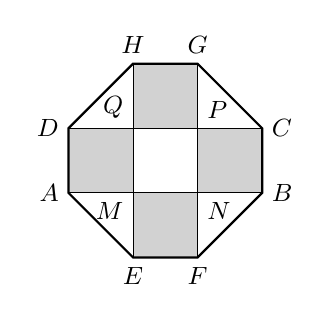
\begin{tikzpicture}[scale=0.82, every node/.style={font=\small}]
  \fill[gray!35] (-1.5,-0.5) rectangle (1.5,0.5);
  \fill[gray!35] (-0.5,-1.5) rectangle (0.5,1.5);
  % 中心正方形 MNPQ 原卷不涂阴影，照原卷留白：
  \fill[white] (-0.5,-0.5) rectangle (0.5,0.5);
  \draw[thick] (-1.5,0.5)--(-0.5,1.5)--(0.5,1.5)--(1.5,0.5)--(1.5,-0.5)--(0.5,-1.5)--(-0.5,-1.5)--(-1.5,-0.5)--cycle;
  \draw (-1.5,-0.5) rectangle (1.5,0.5);
  \draw (-0.5,-1.5) rectangle (0.5,1.5);
  \node[left] at (-1.5,0.5) {$D$};
  \node[left] at (-1.5,-0.5) {$A$};
  \node[right] at (1.5,0.5) {$C$};
  \node[right] at (1.5,-0.5) {$B$};
  \node[above] at (-0.5,1.5) {$H$};
  \node[above] at (0.5,1.5) {$G$};
  \node[below] at (-0.5,-1.5) {$E$};
  \node[below] at (0.5,-1.5) {$F$};
  \node[below left] at (-0.5,-0.5) {$M$};
  \node[below right] at (0.5,-0.5) {$N$};
  \node[above right] at (0.5,0.5) {$P$};
  \node[above left] at (-0.5,0.5) {$Q$};
\end{tikzpicture}
\end{center}

\begin{enumerate}[label=(\arabic*)]
\item 设 $DQ$ 长为 $y$（单位：m），用 $x$ 表示 $y$，并求出 $x$ 的取值范围；
\item $AD$ 取何值时可使总造价最低，并求出最低造价.
\end{enumerate}

\ifanswer
\solbegin
\stepm{(1)}{设 $AD=x\text{m}$（$x>0$），$DQ=y\text{m}$（$y>0$），}
\step{因为十字形区域总面积为 $200\text{m}^2$，所以 $4xy+x^2=200$，}
\step{解得 $y=\dfrac{200-x^2}{4x}=\dfrac{50}{x}-\dfrac{x}{4}$，}
\step{因为 $x>0$，$y>0$，所以 $y=\dfrac{200-x^2}{4x}>0$，解得 $0<x<10\sqrt2$，}
\step{所以 $y=\dfrac{50}{x}-\dfrac{x}{4}$，$0<x<10\sqrt2$；}
\stepm{(2)}{中心正方形 $MNPQ$ 区域，造价为 $2100$ 元$/\text{m}^2$，}
\step{中心正方形 $MNPQ$ 面积为 $S_1=x^2$，造价为 $W_1=2100\times S_1=2100x^2$；}
\step{周围四个矩形区域（图中阴影部分）铺设透水地砖，造价为 $105$ 元$/\text{m}^2$，}
\step{四个矩形的总面积为 $S_2=4xy=4x\left(\dfrac{50}{x}-\dfrac{x}{4}\right)=200-x^2$，}
\step{造价为 $W_2=105\times S_2=105(200-x^2)=21000-105x^2$；}
\step{四个三角形区域种植耐旱固碳植物，助力碳中和，造价为 $40$ 元$/\text{m}^2$，}
\step{四个三角形的总面积为 $S_3=4\times\dfrac12y^2=2\left(\dfrac{50}{x}-\dfrac{x}{4}\right)^2
=\dfrac{5000}{x^2}-50+\dfrac{x^2}{8}$，}
\step{造价为 $W_3=40\times S_3=40\left(\dfrac{5000}{x^2}-50+\dfrac{x^2}{8}\right)
=\dfrac{200000}{x^2}-2000+5x^2$；}
\step{设总造价为 $W$（单位：元），}
\step{则总造价为 $W=W_1+W_2+W_3$}
\step{$=2100x^2+21000-105x^2+\dfrac{200000}{x^2}-2000+5x^2$}
\step{$=2000x^2+\dfrac{200000}{x^2}+19000$，}
\step{又 $2000x^2+\dfrac{200000}{x^2}\geqslant2\sqrt{2000x^2\times\dfrac{200000}{x^2}}=2\times20000=40000$，}
\step{当且仅当 $2000x^2=\dfrac{200000}{x^2}$，即 $x=\sqrt{10}$（在 $x$ 的范围内）时取等号，}
\step{所以 $W=2000x^2+\dfrac{200000}{x^2}+19000\geqslant59000$，当 $x=\sqrt{10}$ 时取等号，}
\step{故当 $AD$ 的长为 $\sqrt{10}$ 时，总造价最低，为 $59000$ 元.}
\solend

\fi

\ansspace[8]

\item 对于实数 $a$、$b$、$c$，若 $|a-c|<|b-c|$，则称 $a$ 比 $b$ 更接近于 $c$. 现已知 $p$、$q$ 都是正有理数.

\begin{enumerate}[label=(\arabic*)]
\item 证明：$\sqrt3$ 必在 $\dfrac pq$ 和 $\dfrac{p+3q}{p+q}$ 之间；
\item 试问 $\dfrac pq$ 和 $\dfrac{p+3q}{p+q}$ 这两个数，哪一个更接近于 $\sqrt3$？说明你的理由；
\item 请你再写出一个有理数，使得它的值比 $\dfrac pq$ 和 $\dfrac{p+3q}{p+q}$ 的值更接近于 $\sqrt3$，并说明你的理由.
\end{enumerate}

\ifanswer
\solbegin
\stepm{(1)}{设 $a=\dfrac pq$（$a$ 为正有理数），则需证 $\sqrt3$ 在 $a$ 和 $\dfrac{a+3}{a+1}$（即 $\dfrac{p+3q}{p+q}$）之间.}
\step{当 $a>\sqrt3$ 时，计算 $a-\dfrac{a+3}{a+1}$ 得 $a-\dfrac{a+3}{a+1}=\dfrac{a(a+1)-(a+3)}{a+1}=\dfrac{a^2-3}{a+1}$，}
\step{$a>\sqrt3$，则 $a^2-3>0$，故 $a>\dfrac{a+3}{a+1}$；}
\step{再计算 $\dfrac{a+3}{a+1}-\sqrt3$ 得 $\dfrac{a+3}{a+1}-\sqrt3=\dfrac{(1-\sqrt3)(a-\sqrt3)}{a+1}$，}
\step{$1-\sqrt3<0$，$a-\sqrt3>0$，$a+1>0$，}
\step{故 $\dfrac{a+3}{a+1}-\sqrt3<0$，即 $\dfrac{a+3}{a+1}<\sqrt3$，从而 $\dfrac{a+3}{a+1}<\sqrt3<a$；}
\step{当 $a<\sqrt3$ 时，同理可得 $a<\dfrac{a+3}{a+1}$ 且 $\dfrac{a+3}{a+1}>\sqrt3$，即 $a<\sqrt3<\dfrac{a+3}{a+1}$，}
\step{综上，$\sqrt3$ 必在 $\dfrac pq$ 和 $\dfrac{p+3q}{p+q}$ 之间；}
\stepm{(2)}{设 $a=\dfrac pq$，$b=\dfrac{p+3q}{p+q}=\dfrac{a+3}{a+1}$，比较 $|a-\sqrt3|$ 与 $|b-\sqrt3|$，}
\step{由（1）得 $(a-\sqrt3)(b-\sqrt3)<0$，}
\step{$\dfrac{|b-\sqrt3|}{|a-\sqrt3|}
=\left|\dfrac{b-\sqrt3}{a-\sqrt3}\right|
=\dfrac{\left|\dfrac{(1-\sqrt3)(a-\sqrt3)}{a+1}\right|}{|a-\sqrt3|}
=\dfrac{\sqrt3-1}{a+1}$，}
\step{$a>0$，$a+1>1$，$\sqrt3-1<1$，故 $\dfrac{\sqrt3-1}{a+1}<1$，即 $|b-\sqrt3|<|a-\sqrt3|$，}
\step{即 $\dfrac{p+3q}{p+q}$ 比 $\dfrac pq$ 更接近于 $\sqrt3$；}
\stepm{(3)}{$\dfrac{2p+3q}{p+2q}$，理由：}
\step{设 $b=\dfrac{p+3q}{p+q}$，新数 $c=\dfrac{b+3}{b+1}=\dfrac{2p+3q}{p+2q}$，}
\step{由（1）得 $(b-\sqrt3)(c-\sqrt3)<0$，}
\step{$c-\sqrt3=\dfrac{b+3}{b+1}-\sqrt3=\dfrac{(1-\sqrt3)(b-\sqrt3)}{b+1}$，}
\step{则 $\dfrac{|c-\sqrt3|}{|b-\sqrt3|}
=\left|\dfrac{c-\sqrt3}{b-\sqrt3}\right|
=\dfrac{\left|\dfrac{(1-\sqrt3)(b-\sqrt3)}{b+1}\right|}{|b-\sqrt3|}
=\dfrac{\sqrt3-1}{b+1}$，}
\step{$b>0$，$b+1>1$，$0<\sqrt3-1<1$，故 $\dfrac{\sqrt3-1}{b+1}<1$，即 $|c-\sqrt3|<|b-\sqrt3|$，}
\step{即 $\dfrac{2p+3q}{p+2q}$ 比 $\dfrac{p+3q}{p+q}$ 更接近于 $\sqrt3$，故 $c$ 更接近 $\sqrt3$.}
\solend

\fi

\ansspace*[10]

\end{enumerate}

\end{document}
"
%
% 原始材料是微信公众号图文（公众号“魔都数学加油站”，作者“破晓”，2026-10-02 17:56 发布，
% 连载“27学年高一45”，原文标题“27学年高一45——2026-2027年上海市交附闵行高一上国庆作业2”，
% https://mp.weixin.qq.com/s/1xdCtzH-3Il0jJrz3saiPA），正文为 10 张 PNG 页。
% 第 01—06、09 页为 4762×6735；第 07、08、10 页为 2560×3620（同一篇各页原图分辨率不一致）。
% 原文本身是一份讲评版：第 3—21 题均照原卷保留题目与题下解析；第 13 题原卷把答案 C 印在括号中。
% 题目、选项、答案与解析均照原卷录入，未改内容；卷面的粉色斜水印及页脚不录入。
%
% 卷首标题：原卷印作“2026-2027 年交附闵行高一上国庆作业 2”（公众号标题里的“上海市”
% 三字卷面标题行没有，本稿照卷面），年份区间按全稿惯例排 en dash，前缀照原卷保留“年”。
%
% 与原卷的排版差异：
%   ① 原卷印有“一、填空题”“二、选择题”“三、解答题”三节标题，本稿照原卷分节，
%      只把标题改排成全稿统一的“大节标题”样式；
%   ② 第 13 题原卷在题干括号内直接印答案 C，本稿按全稿样式将括号留空、答案移入答案版的 \ans{}；
%   ③ 原卷填空横线及选择题答案括号均按全稿样式排版，填空横线统一用 \blankline[4.4em]；
%   ④ 原卷第 20 题配有十字形广场示意图，本稿在源码中用 TikZ 重绘，图中区域、边界及点名照原卷。
%   ⑤ 原卷未印副标题，本稿按本卷实际涉及的知识模块补出“集合与常用逻辑用语、不等式”。
%
% 原卷存疑/错误（均照抄原卷、未改，见对应题目处上方注释）：
%   ① 第 11 题解析原卷印"所以 p=3+9=12，又 12,15∉A，所以 12,15∉B"，与 A∪\overline{B} 的条件
%      及后文 B 的根为 6、9 均一致，无矛盾，本稿照录（早前记录的"∈B／前后矛盾"系本稿误读）；
%   ② 第 15 题题干与解析均按原卷印 ac<0，解析"因为 a<b<c，且 ac<0，所以 a<0，c>0"与题设一致，
%      无矛盾（早前记录的"abc<0／解析冲突"系本稿误读题干所致）；本稿照录原卷答案与解析。
%   ③ 第 20 题原卷各数（造价 2100 元/m^2、W_1=2100x^2、合并式 2000x^2+200000/x^2+19000、
%      末句 59000 元）经复核自洽，无矛盾（早前记录的"W_1=200x^2／末句 5900 元"系本稿误录）；本稿照录。
%   ④ 第 18(2) 题 a=-1 时 A=B=(-1,1)，不满足“B 是 A 的真子集”，故原解析给出的 a≤-1 应为 a<-1；
%   ⑤ 第 19(2) 题原卷用"{c|0<c<1}∩{c|c<-2√3/3 或 c>2√3/3}=∅"论证"不等式①、②中至多有一个恒成立"，
%      论证成立（早前记录的"区间并集留有间隙"系本稿误录解析所致）；本稿照录原卷。
%
\documentclass[a4paper,11pt]{article}
\usepackage{common}

\begin{document}

\examtitlest[3]{2026--2027 年交附闵行高一上国庆作业 2}{集合与常用逻辑用语、不等式}

\bigsec{一、填空题}

\begin{enumerate}
\setcounter{enumi}{2}

\item 满足 $A\cup\{-1,1\}=\{-1,0,1\}$ 的集合 $A$ 共有 \blankline[4.4em] 个.

\ifanswer
\solbegin
\step{集合可能为 $\{0\}$、$\{0,1\}$、$\{0,-1\}$、$\{0,1,-1\}$，共有 $4$ 个.}
\solend

\fi

\item 设 $x\in\R$，则“$x+\dfrac1x>2$”是“$x\neq1$”的 \blankline[4.4em] 条件.

\ifanswer
\solbegin
\step{$x+\dfrac1x>2\Longleftrightarrow x>0$ 且 $x\neq1$，故为充分不必要条件.}
\solend

\fi

\item 已知集合 $A=\{x\mid|x-1|<a\}$，$B=\{-4,3\}$，若 $A\cap B=\varnothing$，则 $a$ 的最大值为 \blankline[4.4em].

\ifanswer
\solbegin
\step{$A=\{x\mid -a<x-1<a\}=\{x\mid1-a<x<1+a\}$，$B=\{-4,3\}$，且 $A\cap B=\varnothing$，}
\step{$A=\varnothing$ 时，$1-a\geqslant1+a$，解得 $a\leqslant0$，满足 $A\cap B=\varnothing$；}
\step{若 $-4\in A$，则 $1-a<-4<1+a$，解得 $a>5$；}
\step{若 $3\in A$，则 $1-a<3<1+a$，解得 $a>2$，}
\step{因为 $A\cap B=\varnothing$，所以 $-4\notin A$ 且 $3\notin A$，所以 $a\leqslant5$ 且 $a\leqslant2$，所以 $a\leqslant2$，}
\step{综上，$a$ 的最大值为 $2$.}
\solend

\fi

\item 设 $x\in\R$，方程 $|x-1|+|2x-1|=|3x-2|$ 的解集为 \blankline[4.4em].

\ifanswer
\solbegin
\step{因为 $|x-1|+|2x-1|\geqslant|(x-1)+(2x-1)|=|3x-2|$，}
\step{当且仅当 $(x-1)(2x-1)\geqslant0$，解得 $x\leqslant\dfrac12$ 或 $x\geqslant1$，}
\step{故方程 $|x-1|+|2x-1|=|3x-2|$ 的解集为 $\left(-\infty,\dfrac12\right]\cup[1,+\infty)$.}
\solend

\fi

\item 已知 $a$、$b\in\R$，且 $3a+2b=1$，则 $8^a+4^b$ 最小值为 \blankline[4.4em].

\ifanswer
\solbegin
% 注：原卷本行与上行均作“$8^a+4^b$ 最小值为”，“最小值”前无“的”，原卷如此，照录未改。
\step{因为 $3a+2b=1$，所以 $8^a+4^b=2^{3a}+2^{2b}\geqslant2\sqrt{2^{3a+2b}}=2\sqrt2$，}
\step{当且仅当 $3a=2b$ 时取等号，故 $8^a+4^b$ 最小值为 $2\sqrt2$.}
\solend

\fi

\item 已知 $a>0$，$b>0$，且 $a+2b+ab=30$，则 $2a+b$ 的最小值为 \blankline[4.4em].

\ifanswer
\solbegin
\step{由 $a+2b+ab=30$，得 $(a+2)(b+1)=32$.}
\step{因为 $a>0$，$b>0$，所以 $a+2>0$，$b+1>0$，}
\step{所以 $2a+b=2(a+2)+(b+1)-5\geqslant2\sqrt{2\times32}-5=11$，}
\step{当且仅当 $2(a+2)=(b+1)$，即 $a=2$，$b=7$ 时取等号，}
\step{所以 $2a+b$ 的最小值为 $11$.}
\solend

\fi

\item 已知 $A=\{x\mid x^2+px+1=0\}$，$M=\{x\mid x>0\}$，若 $A\cap M=\varnothing$，则实数 $p$ 的取值范围为 \blankline[4.4em].

\ifanswer
\solbegin
\step{①当 $A=\varnothing$ 时，$\Delta=p^2-4<0$，所以 $-2<p<2$，此时满足 $A\cap M=\varnothing$；}
\step{②当 $A\neq\varnothing$ 时，$\Delta=p^2-4\geqslant0$，$p\geqslant2$ 或 $p\leqslant-2$，}
\step{因为 $M=\{x\mid x>0\}$，$A\cap M=\varnothing$，由韦达定理得 $\begin{cases}-p\leqslant0\\1>0\end{cases}$，解得 $p\geqslant0$，}
\step{所以 $p\geqslant2$，}
\step{由①②综合得 $p>-2$，故实数 $p$ 的取值范围为 $(-2,+\infty)$.}
\solend

\fi

\item 已知集合 $A=[t,t+1]\cup[t+3,t+6]$，其中 $t>0$. 若存在正数 $\lambda$，使得对任意 $a\in A$，都有 $\dfrac{\lambda}{a}\in A$，则 $t$ 的取值集合为 \blankline[4.4em].

\ifanswer
\solbegin
\step{因为 $0\notin A$，$t>0$，所以 $a\in[t,t+1]\cup[t+3,t+6]$，}
\step{则 $\dfrac1a\in\left[\dfrac1{t+6},\dfrac1{t+3}\right]\cup\left[\dfrac1{t+1},\dfrac1t\right]$，}
\step{又因为 $\lambda>0$，所以 $\dfrac{\lambda}{a}\in\left[\dfrac{\lambda}{t+6},\dfrac{\lambda}{t+3}\right]\cup\left[\dfrac{\lambda}{t+1},\dfrac{\lambda}{t}\right]$，}
\step{因为 $\dfrac{\lambda}{a}\in A$，所以 $\begin{cases}\dfrac{\lambda}{t+6}\geqslant t\\[3pt]\dfrac{\lambda}{t+3}\leqslant t+1\end{cases}$ 且 $\begin{cases}\dfrac{\lambda}{t+1}\geqslant t+3\\[3pt]\dfrac{\lambda}{t}\leqslant t+6\end{cases}$，}
% 注：原卷本行两个不等式组印作“$t(t+6)\leqslant\lambda\leqslant t(t+6)$”与
%     “$(t+1)(t+3)\leqslant\lambda\leqslant(t+1)(t+3)$”（两侧同式），与上行两式推导不合，系原卷笔误；
%     原卷如此，照录未改。
\step{得 $\begin{cases}t(t+6)\leqslant\lambda\leqslant t(t+6)\\[3pt](t+1)(t+3)\leqslant\lambda\leqslant(t+1)(t+3)\end{cases}$，所以 $\lambda=t(t+6)=(t+1)(t+3)$，}
\step{解得 $t=\dfrac32$，取值集合为 $\left\{\dfrac32\right\}$.}
\solend

\fi

\item 已知全集 $U=\{x\mid x=3n,1\leqslant n\leqslant5\ \text{且}\ n\in\N\}$，$A=\{x\mid x^2-px+27=0,p\in\N\}$，
$B=\{x\mid x^2-15x+q=0,q\in\N\}$，且 $A\cup\overline{B}=\{3,9,12,15\}$，则 $p+q$ 的值为 \blankline[4.4em].

\ifanswer
\solbegin
\step{因为全集 $U=\{3,6,9,12,15\}$，$A\cup\overline{B}=\{3,9,12,15\}$，}
\step{所以 $3$、$9$、$12$、$15$ 中可能有两个属于 $A$，}
\step{因为 $A$ 中的方程 $x^2-px+27=0$ 中，两根之积 $x_1x_2=27$，所以 $3$、$9\in A$，}
\step{所以 $p=3+9=12$，又 $12$、$15\notin A$，所以 $12$、$15\notin B$，}
\step{因为 $B$ 中的方程 $x^2-15x+q=0$ 中，两根之和 $x_3+x_4=15$，所以 $6$、$9\in B$，}
\step{则 $q=6\times9=54$，所以 $p+q=66$.}
\solend

\fi

\item 若关于 $x$ 的不等式 $|x-2k|+|x-3k|<4k$ 共有 $2025$ 个整数解，则实数 $k$ 的取值范围为 \blankline[4.4em].

\ifanswer
\solbegin
\step{显然 $k>0$，由 $|x-2k|+|x-3k|<4k$，得 $\dfrac{k}{2}<x<\dfrac{9k}{2}$，}
\step{因为该不等式共有 $2025$ 个整数解，所以 $2024<\dfrac{9k}{2}-\dfrac{k}{2}\leqslant2026$，}
\step{解得 $506<k\leqslant506.5$，}
\step{由 $\dfrac{k}{2}\in(253,253.25]$，得这 $2025$ 个整数解只能为 $254,255,256,\cdots,2278$，}
\step{所以 $2278<\dfrac{9k}{2}\leqslant2279$，解得 $506\dfrac29<k\leqslant506\dfrac49$，结合 $506<k\leqslant506.5$，}
\step{得 $k$ 的取值范围是 $\left(506\dfrac29,506\dfrac49\right]$.}
\solend

\fi

\end{enumerate}

\bigsec{二、选择题}

\begin{enumerate}
\setcounter{enumi}{12}

\item 已知 $a,b\in\R$，且 $ab\neq0$，则下列结论恒成立的是\mbox{（\quad）}

\keepwithprev
A. $a+b\geqslant2\sqrt{ab}$\qquad
B. $\left(\dfrac{a+b}{2}\right)^2>ab$\qquad
C. $\left|\dfrac ab+\dfrac ba\right|\geqslant2$\qquad
D. $a^2+b^2>2ab$

\ans{$C$}

\item 如果 $a^{2025}+b^{2025}=0$，那么一定有\mbox{（\quad）}

\keepwithprev
A. $(|a|+|b|)^{2025}=0$\qquad
B. $(a-b)^{2025}=0$\qquad
C. $(a\cdot b)^{2025}=0$\qquad
D. $(a+b)^{2025}=0$

\ans{$D$}

\ifanswer
\solbegin
\step{由 $a^{2025}+b^{2025}=0$，得 $a^{2025}=-b^{2025}=(-b)^{2025}$，则 $\left(a^{2025}\right)^{\frac{1}{2025}}=\left[(-b)^{2025}\right]^{\frac{1}{2025}}$，}
\step{即 $a=-b$，即 $a+b=0$，故 $(a+b)^{2025}=0$，故 D 符合题意；}
\step{对于 A，若取 $a=1$，$b=-1$，则 $(|a|+|b|)^{2025}=2^{2025}\neq0$，故 A 不合题意；}
\step{对于 B，若取 $a=1$，$b=-1$，则 $(a-b)^{2025}=2^{2025}\neq0$，故 B 不合题意；}
\step{对于 C，若取 $a=1$，$b=-1$，则 $(a\cdot b)^{2025}=(-1)^{2025}=-1\neq0$，故 C 不合题意；}
\step{故选 D.}
\solend

\fi

\item 已知 $a$、$b$、$c$ 满足 $a<b<c$，且 $ac<0$，那么下列各式中一定成立的是\mbox{（\quad）}

\keepwithprev
A. $\dfrac1a>\dfrac1c$\qquad
B. $ab^2<cb^2$\qquad
C. $ac<bc$\qquad
D. $a+c>2b$

\ans{$C$}

\ifanswer
\solbegin
\step{因为 $a<b<c$，且 $ac<0$，所以 $a<0$，$c>0$，}
\step{对于 A，$\dfrac1a<0<\dfrac1c$，故 A 错误；}
\step{对于 B，当 $b=0$ 时，$ab^2=cb^2$，故 B 错误；}
\step{对于 C，$ac<bc$ 可化为 $(a-b)c<0$，因为 $a<b$，所以 $a-b<0$，}
\step{又因为 $c>0$，所以 $(a-b)c<0$，所以 C 正确；}
\step{对于 D，设 $a=-2$，$b=0$，$c=1$，则 $a+c<2b$，故 D 错误.}
\step{故选 C.}
\solend

\fi

\item 对于 $a\in\R$，设集合 $A=\left\{x\mid\dfrac{(x^2-6x+a)(x-1)}{x+a}=0\right\}$，记 $A$ 的所有元素之和为 $S(a)$，
所有元素之积为 $T(a)$，则下列说法中，正确的是\mbox{（\quad）}

\keepwithprev
A. 不存在实数 $a$，使得 $S(a)=6$\qquad
B. 存在实数 $a$，使得 $T(a)=9$

C. 存在无数实数 $a$，使得 $S(a)=7$\qquad
D. 若 $T(a)=3$，则 $a=3$

\ans{$C$}

\ifanswer
\solbegin
\step{要使 $\dfrac{(x^2-6x+a)(x-1)}{x+a}=0$，只需 $(x^2-6x+a)(x-1)=0$ 且 $x+a\neq0$，}
\step{由 $(x^2-6x+a)(x-1)=0$ 得 $x^2-6x+a=0$ 或 $x-1=0$，}
\step{对于一元二次方程 $x^2-6x+a=0$，其判别式 $\Delta=36-4a$，}
\step{当 $\Delta=0$，即 $a=9$ 时，集合 $A=\{1,3\}$，$S(a)=4$，$T(a)=3$；}
\step{当 $\Delta<0$，即 $a>9$ 时，集合 $A=\{1\}$，$S(a)=T(a)=1$；}
\step{当 $\Delta>0$，即 $a<9$ 时，一元二次方程 $x^2-6x+a=0$ 的解为 $x=3\pm\sqrt{9-a}$，}
\step{①当 $a=0$ 时，$x\neq0$，则集合 $A=\{1,6\}$，则 $S(a)=7$，$T(a)=6$，}
\step{②当 $a=-7$ 时，$x\neq7$，则集合 $A=\{-1,1\}$，则 $S(a)=0$，$T(a)=-1$，}
% 注：下一行集合 A 原卷印作 {-1,1}（按 a=-1 代入 x^2-6x-1=0 应得 3±√10，原卷如此，照录未改）。
\step{③当 $a=-1$ 时，$x\neq1$，则集合 $A=\{-1,1\}$，则 $S(a)=6$，$T(a)=-1$，}
\step{④当 $a=5$ 时，$x\neq-5$，则集合 $A=\{1,5\}$，则 $S(a)=6$，$T(a)=5$，}
\step{⑤当 $a\neq5,0,-1,-7$ 时，集合 $A=\{1,3-\sqrt{9-a},3+\sqrt{9-a}\}$，}
\step{则 $S(a)=7$，$T(a)=a$.}
\step{选项 A，当 $a=5$ 时，$S(a)=6$，所以 A 错误；}
\step{选项 B，$T(a)$ 的可能值为 $-1,1,3,5,6,a$（$a<9$），无 $T(a)=9$，所以 B 错误；}
\step{选项 C，当 $a<9$，且 $a\neq5,-1,-7$ 时，$S(a)=7$，有无数个 $a$ 满足，所以 C 正确；}
\step{选项 D，当 $T(a)=3$ 时，有 $a=3$ 和 $a=9$ 满足，所以 D 错误.}
\step{故选 C.}
\solend

\fi

\end{enumerate}

\bigsec{三、解答题}

\begin{enumerate}
\setcounter{enumi}{16}

\item 已知 $a\in\R$，关于 $x$ 的不等式 $|x+1|+|x-1|>a^2-5a+4$.

\begin{enumerate}[label=(\arabic*)]
\item 当 $a=0$ 时，求不等式的解集；
\item 若不等式的解集为 $\R$，求 $a$ 的取值范围.
\end{enumerate}

\ifanswer
\solbegin
\stepm{(1)}{当 $a=0$ 时，不等式为 $|x+1|+|x-1|>4$，}
\step{又 $|x+1|+|x-1|=\begin{cases}2x,&x\geqslant1\\2,&-1<x<1\\-2x,&x\leqslant-1\end{cases}$，}
\step{则 $|x+1|+|x-1|>4$ 的解为 $x>2$ 或 $x<-2$，}
\step{即不等式的解集为 $(-\infty,-2)\cup(2,+\infty)$；}
\stepm{(2)}{不等式 $|x+1|+|x-1|>a^2-5a+4$ 的解集为 $\R$，}
\step{则 $(|x+1|+|x-1|)_{\min}>a^2-5a+4$，}
\step{又 $(|x+1|+|x-1|)_{\min}=2$，当且仅当 $-1\leqslant x\leqslant1$ 时取得，即 $a^2-5a+4<2$，}
\step{即 $a^2-5a+2<0$，即 $\dfrac{5-\sqrt{17}}2<a<\dfrac{5+\sqrt{17}}2$，}
\step{即 $a$ 的取值范围为 $\left(\dfrac{5-\sqrt{17}}2,\dfrac{5+\sqrt{17}}2\right)$.}
\solend

\fi

\ansspace[6]

\item 已知集合 $A=\{x\mid(x-a)(x-a^2)<0\}$，集合 $B=\left\{x\mid\dfrac{2x}{x-1}<1\right\}$，命题 $p:x\in A$，命题 $q:x\in B$.

\begin{enumerate}[label=(\arabic*)]
\item 当实数 $a$ 为何值时，$A=B$；
\item 若 $q$ 是 $p$ 的充分不必要条件，求实数 $a$ 的取值范围.
\end{enumerate}

\ifanswer
\solbegin
\stepm{(1)}{由 $\dfrac{2x}{x-1}<1$ 得 $\dfrac{2x}{x-1}-1=\dfrac{x+1}{x-1}<0$，解得 $-1<x<1$，即 $B=\{x\mid-1<x<1\}$，}
\step{因为 $A=\{x\mid(x-a)(x-a^2)<0\}$，$A=B$，所以 $\begin{cases}a=-1\\a^2=1\end{cases}$，解得 $a=-1$；}
\stepm{(2)}{若 $q$ 是 $p$ 的充分不必要条件，则 $B\subset A$，}
\step{当 $a^2=a$，即 $a=0$ 或 $a=1$ 时，$A=\varnothing$，显然不符合题意；}
\step{当 $a^2>a$，即 $a>1$ 或 $a<0$ 时，$A=(a,a^2)$，则 $\begin{cases}a\leqslant-1\\a^2\geqslant1\\a>1\ \text{或}\ a<0\end{cases}$，}
% 注：a=-1 时 A=(-1,1)=B，不是 B 的真子集；原解析用 B⊂A 但答案含 -1，照录。
\step{前两等号不能同时取得，解得 $a\leqslant-1$；}
\step{当 $a^2<a$，即 $0<a<1$ 时，$A=(a^2,a)$，显然不符合题意，}
\step{故 $a$ 的范围为 $\{a\mid a\leqslant-1\}$.}
\solend

\fi

\ansspace[6]

\item 已知不等式① $x^2+2cx+c>0$，② $x^2+cx+c^2-1>0$，其中 $c$ 是实数.

\begin{enumerate}[label=(\arabic*)]
\item 若 $1$ 是不等式②的一个解，求实数 $c$ 的取值范围；
\item 证明：不等式①、②中至多有一个恒成立.
\end{enumerate}

\ifanswer
\solbegin
\stepm{(1)}{已知不等式① $x^2+2cx+c>0$，② $x^2+cx+c^2-1>0$，}
\step{又 $1$ 是不等式②的一个解，则 $1+c+c^2-1>0$，}
\step{则 $c^2+c>0$，则 $c<-1$ 或 $c>0$，则 $c$ 的取值范围为 $(-\infty,-1)\cup(0,+\infty)$；}
\stepm{(2)}{若不等式①恒成立，则 $\Delta=4c^2-4c<0$，则 $0<c<1$，}
\step{若不等式②恒成立，则 $\Delta=c^2-4(c^2-1)=4-3c^2<0$，}
\step{则 $c<-\dfrac{2\sqrt3}{3}$ 或 $c>\dfrac{2\sqrt3}{3}$，}
\step{又 $\{c\mid 0<c<1\}\cap\left\{c\mid c<-\dfrac{2\sqrt3}{3}\ \text{或}\ c>\dfrac{2\sqrt3}{3}\right\}=\varnothing$，}
\step{则不存在实数 $c$ 使得不等式①、②同时恒成立，}
\step{则不等式①、②中至多有一个恒成立.}
\solend

\fi

\ansspace[6]

\item 为践行“科技强国”战略，某社区计划建造一座融合智慧节能技术的八边形休闲广场，其中两个相同的矩形 $ABCD$ 和 $EFGH$ 构成的十字形区域总面积为 $200\text{m}^2$. 中心正方形 $MNPQ$ 区域将安装国产太阳能光伏板（兼具休憩遮阳功能），造价为 $2100$ 元$/\text{m}^2$；周围四个矩形区域（图中阴影部分）铺设透水地砖，造价为 $105$ 元$/\text{m}^2$；再在四个三角形区域种植耐旱固碳植物，助力碳中和，造价为 $40$ 元$/\text{m}^2$. 设总造价为 $W$（单位：元），$AD=x$（单位：m）.

\begin{center}
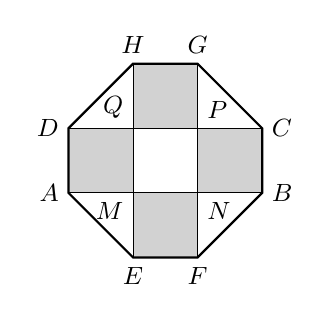
\begin{tikzpicture}[scale=0.82, every node/.style={font=\small}]
  \fill[gray!35] (-1.5,-0.5) rectangle (1.5,0.5);
  \fill[gray!35] (-0.5,-1.5) rectangle (0.5,1.5);
  % 中心正方形 MNPQ 原卷不涂阴影，照原卷留白：
  \fill[white] (-0.5,-0.5) rectangle (0.5,0.5);
  \draw[thick] (-1.5,0.5)--(-0.5,1.5)--(0.5,1.5)--(1.5,0.5)--(1.5,-0.5)--(0.5,-1.5)--(-0.5,-1.5)--(-1.5,-0.5)--cycle;
  \draw (-1.5,-0.5) rectangle (1.5,0.5);
  \draw (-0.5,-1.5) rectangle (0.5,1.5);
  \node[left] at (-1.5,0.5) {$D$};
  \node[left] at (-1.5,-0.5) {$A$};
  \node[right] at (1.5,0.5) {$C$};
  \node[right] at (1.5,-0.5) {$B$};
  \node[above] at (-0.5,1.5) {$H$};
  \node[above] at (0.5,1.5) {$G$};
  \node[below] at (-0.5,-1.5) {$E$};
  \node[below] at (0.5,-1.5) {$F$};
  \node[below left] at (-0.5,-0.5) {$M$};
  \node[below right] at (0.5,-0.5) {$N$};
  \node[above right] at (0.5,0.5) {$P$};
  \node[above left] at (-0.5,0.5) {$Q$};
\end{tikzpicture}
\end{center}

\begin{enumerate}[label=(\arabic*)]
\item 设 $DQ$ 长为 $y$（单位：m），用 $x$ 表示 $y$，并求出 $x$ 的取值范围；
\item $AD$ 取何值时可使总造价最低，并求出最低造价.
\end{enumerate}

\ifanswer
\solbegin
\stepm{(1)}{设 $AD=x\text{m}$（$x>0$），$DQ=y\text{m}$（$y>0$），}
\step{因为十字形区域总面积为 $200\text{m}^2$，所以 $4xy+x^2=200$，}
\step{解得 $y=\dfrac{200-x^2}{4x}=\dfrac{50}{x}-\dfrac{x}{4}$，}
\step{因为 $x>0$，$y>0$，所以 $y=\dfrac{200-x^2}{4x}>0$，解得 $0<x<10\sqrt2$，}
\step{所以 $y=\dfrac{50}{x}-\dfrac{x}{4}$，$0<x<10\sqrt2$；}
\stepm{(2)}{中心正方形 $MNPQ$ 区域，造价为 $2100$ 元$/\text{m}^2$，}
\step{中心正方形 $MNPQ$ 面积为 $S_1=x^2$，造价为 $W_1=2100\times S_1=2100x^2$；}
\step{周围四个矩形区域（图中阴影部分）铺设透水地砖，造价为 $105$ 元$/\text{m}^2$，}
\step{四个矩形的总面积为 $S_2=4xy=4x\left(\dfrac{50}{x}-\dfrac{x}{4}\right)=200-x^2$，}
\step{造价为 $W_2=105\times S_2=105(200-x^2)=21000-105x^2$；}
\step{四个三角形区域种植耐旱固碳植物，助力碳中和，造价为 $40$ 元$/\text{m}^2$，}
\step{四个三角形的总面积为 $S_3=4\times\dfrac12y^2=2\left(\dfrac{50}{x}-\dfrac{x}{4}\right)^2
=\dfrac{5000}{x^2}-50+\dfrac{x^2}{8}$，}
\step{造价为 $W_3=40\times S_3=40\left(\dfrac{5000}{x^2}-50+\dfrac{x^2}{8}\right)
=\dfrac{200000}{x^2}-2000+5x^2$；}
\step{设总造价为 $W$（单位：元），}
\step{则总造价为 $W=W_1+W_2+W_3$}
\step{$=2100x^2+21000-105x^2+\dfrac{200000}{x^2}-2000+5x^2$}
\step{$=2000x^2+\dfrac{200000}{x^2}+19000$，}
\step{又 $2000x^2+\dfrac{200000}{x^2}\geqslant2\sqrt{2000x^2\times\dfrac{200000}{x^2}}=2\times20000=40000$，}
\step{当且仅当 $2000x^2=\dfrac{200000}{x^2}$，即 $x=\sqrt{10}$（在 $x$ 的范围内）时取等号，}
\step{所以 $W=2000x^2+\dfrac{200000}{x^2}+19000\geqslant59000$，当 $x=\sqrt{10}$ 时取等号，}
\step{故当 $AD$ 的长为 $\sqrt{10}$ 时，总造价最低，为 $59000$ 元.}
\solend

\fi

\ansspace[8]

\item 对于实数 $a$、$b$、$c$，若 $|a-c|<|b-c|$，则称 $a$ 比 $b$ 更接近于 $c$. 现已知 $p$、$q$ 都是正有理数.

\begin{enumerate}[label=(\arabic*)]
\item 证明：$\sqrt3$ 必在 $\dfrac pq$ 和 $\dfrac{p+3q}{p+q}$ 之间；
\item 试问 $\dfrac pq$ 和 $\dfrac{p+3q}{p+q}$ 这两个数，哪一个更接近于 $\sqrt3$？说明你的理由；
\item 请你再写出一个有理数，使得它的值比 $\dfrac pq$ 和 $\dfrac{p+3q}{p+q}$ 的值更接近于 $\sqrt3$，并说明你的理由.
\end{enumerate}

\ifanswer
\solbegin
\stepm{(1)}{设 $a=\dfrac pq$（$a$ 为正有理数），则需证 $\sqrt3$ 在 $a$ 和 $\dfrac{a+3}{a+1}$（即 $\dfrac{p+3q}{p+q}$）之间.}
\step{当 $a>\sqrt3$ 时，计算 $a-\dfrac{a+3}{a+1}$ 得 $a-\dfrac{a+3}{a+1}=\dfrac{a(a+1)-(a+3)}{a+1}=\dfrac{a^2-3}{a+1}$，}
\step{$a>\sqrt3$，则 $a^2-3>0$，故 $a>\dfrac{a+3}{a+1}$；}
\step{再计算 $\dfrac{a+3}{a+1}-\sqrt3$ 得 $\dfrac{a+3}{a+1}-\sqrt3=\dfrac{(1-\sqrt3)(a-\sqrt3)}{a+1}$，}
\step{$1-\sqrt3<0$，$a-\sqrt3>0$，$a+1>0$，}
\step{故 $\dfrac{a+3}{a+1}-\sqrt3<0$，即 $\dfrac{a+3}{a+1}<\sqrt3$，从而 $\dfrac{a+3}{a+1}<\sqrt3<a$；}
\step{当 $a<\sqrt3$ 时，同理可得 $a<\dfrac{a+3}{a+1}$ 且 $\dfrac{a+3}{a+1}>\sqrt3$，即 $a<\sqrt3<\dfrac{a+3}{a+1}$，}
\step{综上，$\sqrt3$ 必在 $\dfrac pq$ 和 $\dfrac{p+3q}{p+q}$ 之间；}
\stepm{(2)}{设 $a=\dfrac pq$，$b=\dfrac{p+3q}{p+q}=\dfrac{a+3}{a+1}$，比较 $|a-\sqrt3|$ 与 $|b-\sqrt3|$，}
\step{由（1）得 $(a-\sqrt3)(b-\sqrt3)<0$，}
\step{$\dfrac{|b-\sqrt3|}{|a-\sqrt3|}
=\left|\dfrac{b-\sqrt3}{a-\sqrt3}\right|
=\dfrac{\left|\dfrac{(1-\sqrt3)(a-\sqrt3)}{a+1}\right|}{|a-\sqrt3|}
=\dfrac{\sqrt3-1}{a+1}$，}
\step{$a>0$，$a+1>1$，$\sqrt3-1<1$，故 $\dfrac{\sqrt3-1}{a+1}<1$，即 $|b-\sqrt3|<|a-\sqrt3|$，}
\step{即 $\dfrac{p+3q}{p+q}$ 比 $\dfrac pq$ 更接近于 $\sqrt3$；}
\stepm{(3)}{$\dfrac{2p+3q}{p+2q}$，理由：}
\step{设 $b=\dfrac{p+3q}{p+q}$，新数 $c=\dfrac{b+3}{b+1}=\dfrac{2p+3q}{p+2q}$，}
\step{由（1）得 $(b-\sqrt3)(c-\sqrt3)<0$，}
\step{$c-\sqrt3=\dfrac{b+3}{b+1}-\sqrt3=\dfrac{(1-\sqrt3)(b-\sqrt3)}{b+1}$，}
\step{则 $\dfrac{|c-\sqrt3|}{|b-\sqrt3|}
=\left|\dfrac{c-\sqrt3}{b-\sqrt3}\right|
=\dfrac{\left|\dfrac{(1-\sqrt3)(b-\sqrt3)}{b+1}\right|}{|b-\sqrt3|}
=\dfrac{\sqrt3-1}{b+1}$，}
\step{$b>0$，$b+1>1$，$0<\sqrt3-1<1$，故 $\dfrac{\sqrt3-1}{b+1}<1$，即 $|c-\sqrt3|<|b-\sqrt3|$，}
\step{即 $\dfrac{2p+3q}{p+2q}$ 比 $\dfrac{p+3q}{p+q}$ 更接近于 $\sqrt3$，故 $c$ 更接近 $\sqrt3$.}
\solend

\fi

\ansspace*[10]

\end{enumerate}

\end{document}
"
% 紧凑版：xelatex "\def\iscompact{1}% 高一45_交附闵行_国庆作业2.tex
%   —— 高一上数学“2026-2027 年交附闵行高一上国庆作业 2”（试卷版/答案版）
% 试卷版：xelatex 高一45_交附闵行_国庆作业2.tex
% 答案版：xelatex "\def\isanswer{1}% 高一45_交附闵行_国庆作业2.tex
%   —— 高一上数学“2026-2027 年交附闵行高一上国庆作业 2”（试卷版/答案版）
% 试卷版：xelatex 高一45_交附闵行_国庆作业2.tex
% 答案版：xelatex "\def\isanswer{1}\input{高一45_交附闵行_国庆作业2.tex}"
% 紧凑版：xelatex "\def\iscompact{1}\input{高一45_交附闵行_国庆作业2.tex}"
%
% 原始材料是微信公众号图文（公众号“魔都数学加油站”，作者“破晓”，2026-10-02 17:56 发布，
% 连载“27学年高一45”，原文标题“27学年高一45——2026-2027年上海市交附闵行高一上国庆作业2”，
% https://mp.weixin.qq.com/s/1xdCtzH-3Il0jJrz3saiPA），正文为 10 张 PNG 页。
% 第 01—06、09 页为 4762×6735；第 07、08、10 页为 2560×3620（同一篇各页原图分辨率不一致）。
% 原文本身是一份讲评版：第 3—21 题均照原卷保留题目与题下解析；第 13 题原卷把答案 C 印在括号中。
% 题目、选项、答案与解析均照原卷录入，未改内容；卷面的粉色斜水印及页脚不录入。
%
% 卷首标题：原卷印作“2026-2027 年交附闵行高一上国庆作业 2”（公众号标题里的“上海市”
% 三字卷面标题行没有，本稿照卷面），年份区间按全稿惯例排 en dash，前缀照原卷保留“年”。
%
% 与原卷的排版差异：
%   ① 原卷印有“一、填空题”“二、选择题”“三、解答题”三节标题，本稿照原卷分节，
%      只把标题改排成全稿统一的“大节标题”样式；
%   ② 第 13 题原卷在题干括号内直接印答案 C，本稿按全稿样式将括号留空、答案移入答案版的 \ans{}；
%   ③ 原卷填空横线及选择题答案括号均按全稿样式排版，填空横线统一用 \blankline[4.4em]；
%   ④ 原卷第 20 题配有十字形广场示意图，本稿在源码中用 TikZ 重绘，图中区域、边界及点名照原卷。
%   ⑤ 原卷未印副标题，本稿按本卷实际涉及的知识模块补出“集合与常用逻辑用语、不等式”。
%
% 原卷存疑/错误（均照抄原卷、未改，见对应题目处上方注释）：
%   ① 第 11 题解析原卷印"所以 p=3+9=12，又 12,15∉A，所以 12,15∉B"，与 A∪\overline{B} 的条件
%      及后文 B 的根为 6、9 均一致，无矛盾，本稿照录（早前记录的"∈B／前后矛盾"系本稿误读）；
%   ② 第 15 题题干与解析均按原卷印 ac<0，解析"因为 a<b<c，且 ac<0，所以 a<0，c>0"与题设一致，
%      无矛盾（早前记录的"abc<0／解析冲突"系本稿误读题干所致）；本稿照录原卷答案与解析。
%   ③ 第 20 题原卷各数（造价 2100 元/m^2、W_1=2100x^2、合并式 2000x^2+200000/x^2+19000、
%      末句 59000 元）经复核自洽，无矛盾（早前记录的"W_1=200x^2／末句 5900 元"系本稿误录）；本稿照录。
%   ④ 第 18(2) 题 a=-1 时 A=B=(-1,1)，不满足“B 是 A 的真子集”，故原解析给出的 a≤-1 应为 a<-1；
%   ⑤ 第 19(2) 题原卷用"{c|0<c<1}∩{c|c<-2√3/3 或 c>2√3/3}=∅"论证"不等式①、②中至多有一个恒成立"，
%      论证成立（早前记录的"区间并集留有间隙"系本稿误录解析所致）；本稿照录原卷。
%
\documentclass[a4paper,11pt]{article}
\usepackage{common}

\begin{document}

\examtitlest[3]{2026--2027 年交附闵行高一上国庆作业 2}{集合与常用逻辑用语、不等式}

\bigsec{一、填空题}

\begin{enumerate}
\setcounter{enumi}{2}

\item 满足 $A\cup\{-1,1\}=\{-1,0,1\}$ 的集合 $A$ 共有 \blankline[4.4em] 个.

\ifanswer
\solbegin
\step{集合可能为 $\{0\}$、$\{0,1\}$、$\{0,-1\}$、$\{0,1,-1\}$，共有 $4$ 个.}
\solend

\fi

\item 设 $x\in\R$，则“$x+\dfrac1x>2$”是“$x\neq1$”的 \blankline[4.4em] 条件.

\ifanswer
\solbegin
\step{$x+\dfrac1x>2\Longleftrightarrow x>0$ 且 $x\neq1$，故为充分不必要条件.}
\solend

\fi

\item 已知集合 $A=\{x\mid|x-1|<a\}$，$B=\{-4,3\}$，若 $A\cap B=\varnothing$，则 $a$ 的最大值为 \blankline[4.4em].

\ifanswer
\solbegin
\step{$A=\{x\mid -a<x-1<a\}=\{x\mid1-a<x<1+a\}$，$B=\{-4,3\}$，且 $A\cap B=\varnothing$，}
\step{$A=\varnothing$ 时，$1-a\geqslant1+a$，解得 $a\leqslant0$，满足 $A\cap B=\varnothing$；}
\step{若 $-4\in A$，则 $1-a<-4<1+a$，解得 $a>5$；}
\step{若 $3\in A$，则 $1-a<3<1+a$，解得 $a>2$，}
\step{因为 $A\cap B=\varnothing$，所以 $-4\notin A$ 且 $3\notin A$，所以 $a\leqslant5$ 且 $a\leqslant2$，所以 $a\leqslant2$，}
\step{综上，$a$ 的最大值为 $2$.}
\solend

\fi

\item 设 $x\in\R$，方程 $|x-1|+|2x-1|=|3x-2|$ 的解集为 \blankline[4.4em].

\ifanswer
\solbegin
\step{因为 $|x-1|+|2x-1|\geqslant|(x-1)+(2x-1)|=|3x-2|$，}
\step{当且仅当 $(x-1)(2x-1)\geqslant0$，解得 $x\leqslant\dfrac12$ 或 $x\geqslant1$，}
\step{故方程 $|x-1|+|2x-1|=|3x-2|$ 的解集为 $\left(-\infty,\dfrac12\right]\cup[1,+\infty)$.}
\solend

\fi

\item 已知 $a$、$b\in\R$，且 $3a+2b=1$，则 $8^a+4^b$ 最小值为 \blankline[4.4em].

\ifanswer
\solbegin
% 注：原卷本行与上行均作“$8^a+4^b$ 最小值为”，“最小值”前无“的”，原卷如此，照录未改。
\step{因为 $3a+2b=1$，所以 $8^a+4^b=2^{3a}+2^{2b}\geqslant2\sqrt{2^{3a+2b}}=2\sqrt2$，}
\step{当且仅当 $3a=2b$ 时取等号，故 $8^a+4^b$ 最小值为 $2\sqrt2$.}
\solend

\fi

\item 已知 $a>0$，$b>0$，且 $a+2b+ab=30$，则 $2a+b$ 的最小值为 \blankline[4.4em].

\ifanswer
\solbegin
\step{由 $a+2b+ab=30$，得 $(a+2)(b+1)=32$.}
\step{因为 $a>0$，$b>0$，所以 $a+2>0$，$b+1>0$，}
\step{所以 $2a+b=2(a+2)+(b+1)-5\geqslant2\sqrt{2\times32}-5=11$，}
\step{当且仅当 $2(a+2)=(b+1)$，即 $a=2$，$b=7$ 时取等号，}
\step{所以 $2a+b$ 的最小值为 $11$.}
\solend

\fi

\item 已知 $A=\{x\mid x^2+px+1=0\}$，$M=\{x\mid x>0\}$，若 $A\cap M=\varnothing$，则实数 $p$ 的取值范围为 \blankline[4.4em].

\ifanswer
\solbegin
\step{①当 $A=\varnothing$ 时，$\Delta=p^2-4<0$，所以 $-2<p<2$，此时满足 $A\cap M=\varnothing$；}
\step{②当 $A\neq\varnothing$ 时，$\Delta=p^2-4\geqslant0$，$p\geqslant2$ 或 $p\leqslant-2$，}
\step{因为 $M=\{x\mid x>0\}$，$A\cap M=\varnothing$，由韦达定理得 $\begin{cases}-p\leqslant0\\1>0\end{cases}$，解得 $p\geqslant0$，}
\step{所以 $p\geqslant2$，}
\step{由①②综合得 $p>-2$，故实数 $p$ 的取值范围为 $(-2,+\infty)$.}
\solend

\fi

\item 已知集合 $A=[t,t+1]\cup[t+3,t+6]$，其中 $t>0$. 若存在正数 $\lambda$，使得对任意 $a\in A$，都有 $\dfrac{\lambda}{a}\in A$，则 $t$ 的取值集合为 \blankline[4.4em].

\ifanswer
\solbegin
\step{因为 $0\notin A$，$t>0$，所以 $a\in[t,t+1]\cup[t+3,t+6]$，}
\step{则 $\dfrac1a\in\left[\dfrac1{t+6},\dfrac1{t+3}\right]\cup\left[\dfrac1{t+1},\dfrac1t\right]$，}
\step{又因为 $\lambda>0$，所以 $\dfrac{\lambda}{a}\in\left[\dfrac{\lambda}{t+6},\dfrac{\lambda}{t+3}\right]\cup\left[\dfrac{\lambda}{t+1},\dfrac{\lambda}{t}\right]$，}
\step{因为 $\dfrac{\lambda}{a}\in A$，所以 $\begin{cases}\dfrac{\lambda}{t+6}\geqslant t\\[3pt]\dfrac{\lambda}{t+3}\leqslant t+1\end{cases}$ 且 $\begin{cases}\dfrac{\lambda}{t+1}\geqslant t+3\\[3pt]\dfrac{\lambda}{t}\leqslant t+6\end{cases}$，}
% 注：原卷本行两个不等式组印作“$t(t+6)\leqslant\lambda\leqslant t(t+6)$”与
%     “$(t+1)(t+3)\leqslant\lambda\leqslant(t+1)(t+3)$”（两侧同式），与上行两式推导不合，系原卷笔误；
%     原卷如此，照录未改。
\step{得 $\begin{cases}t(t+6)\leqslant\lambda\leqslant t(t+6)\\[3pt](t+1)(t+3)\leqslant\lambda\leqslant(t+1)(t+3)\end{cases}$，所以 $\lambda=t(t+6)=(t+1)(t+3)$，}
\step{解得 $t=\dfrac32$，取值集合为 $\left\{\dfrac32\right\}$.}
\solend

\fi

\item 已知全集 $U=\{x\mid x=3n,1\leqslant n\leqslant5\ \text{且}\ n\in\N\}$，$A=\{x\mid x^2-px+27=0,p\in\N\}$，
$B=\{x\mid x^2-15x+q=0,q\in\N\}$，且 $A\cup\overline{B}=\{3,9,12,15\}$，则 $p+q$ 的值为 \blankline[4.4em].

\ifanswer
\solbegin
\step{因为全集 $U=\{3,6,9,12,15\}$，$A\cup\overline{B}=\{3,9,12,15\}$，}
\step{所以 $3$、$9$、$12$、$15$ 中可能有两个属于 $A$，}
\step{因为 $A$ 中的方程 $x^2-px+27=0$ 中，两根之积 $x_1x_2=27$，所以 $3$、$9\in A$，}
\step{所以 $p=3+9=12$，又 $12$、$15\notin A$，所以 $12$、$15\notin B$，}
\step{因为 $B$ 中的方程 $x^2-15x+q=0$ 中，两根之和 $x_3+x_4=15$，所以 $6$、$9\in B$，}
\step{则 $q=6\times9=54$，所以 $p+q=66$.}
\solend

\fi

\item 若关于 $x$ 的不等式 $|x-2k|+|x-3k|<4k$ 共有 $2025$ 个整数解，则实数 $k$ 的取值范围为 \blankline[4.4em].

\ifanswer
\solbegin
\step{显然 $k>0$，由 $|x-2k|+|x-3k|<4k$，得 $\dfrac{k}{2}<x<\dfrac{9k}{2}$，}
\step{因为该不等式共有 $2025$ 个整数解，所以 $2024<\dfrac{9k}{2}-\dfrac{k}{2}\leqslant2026$，}
\step{解得 $506<k\leqslant506.5$，}
\step{由 $\dfrac{k}{2}\in(253,253.25]$，得这 $2025$ 个整数解只能为 $254,255,256,\cdots,2278$，}
\step{所以 $2278<\dfrac{9k}{2}\leqslant2279$，解得 $506\dfrac29<k\leqslant506\dfrac49$，结合 $506<k\leqslant506.5$，}
\step{得 $k$ 的取值范围是 $\left(506\dfrac29,506\dfrac49\right]$.}
\solend

\fi

\end{enumerate}

\bigsec{二、选择题}

\begin{enumerate}
\setcounter{enumi}{12}

\item 已知 $a,b\in\R$，且 $ab\neq0$，则下列结论恒成立的是\mbox{（\quad）}

\keepwithprev
A. $a+b\geqslant2\sqrt{ab}$\qquad
B. $\left(\dfrac{a+b}{2}\right)^2>ab$\qquad
C. $\left|\dfrac ab+\dfrac ba\right|\geqslant2$\qquad
D. $a^2+b^2>2ab$

\ans{$C$}

\item 如果 $a^{2025}+b^{2025}=0$，那么一定有\mbox{（\quad）}

\keepwithprev
A. $(|a|+|b|)^{2025}=0$\qquad
B. $(a-b)^{2025}=0$\qquad
C. $(a\cdot b)^{2025}=0$\qquad
D. $(a+b)^{2025}=0$

\ans{$D$}

\ifanswer
\solbegin
\step{由 $a^{2025}+b^{2025}=0$，得 $a^{2025}=-b^{2025}=(-b)^{2025}$，则 $\left(a^{2025}\right)^{\frac{1}{2025}}=\left[(-b)^{2025}\right]^{\frac{1}{2025}}$，}
\step{即 $a=-b$，即 $a+b=0$，故 $(a+b)^{2025}=0$，故 D 符合题意；}
\step{对于 A，若取 $a=1$，$b=-1$，则 $(|a|+|b|)^{2025}=2^{2025}\neq0$，故 A 不合题意；}
\step{对于 B，若取 $a=1$，$b=-1$，则 $(a-b)^{2025}=2^{2025}\neq0$，故 B 不合题意；}
\step{对于 C，若取 $a=1$，$b=-1$，则 $(a\cdot b)^{2025}=(-1)^{2025}=-1\neq0$，故 C 不合题意；}
\step{故选 D.}
\solend

\fi

\item 已知 $a$、$b$、$c$ 满足 $a<b<c$，且 $ac<0$，那么下列各式中一定成立的是\mbox{（\quad）}

\keepwithprev
A. $\dfrac1a>\dfrac1c$\qquad
B. $ab^2<cb^2$\qquad
C. $ac<bc$\qquad
D. $a+c>2b$

\ans{$C$}

\ifanswer
\solbegin
\step{因为 $a<b<c$，且 $ac<0$，所以 $a<0$，$c>0$，}
\step{对于 A，$\dfrac1a<0<\dfrac1c$，故 A 错误；}
\step{对于 B，当 $b=0$ 时，$ab^2=cb^2$，故 B 错误；}
\step{对于 C，$ac<bc$ 可化为 $(a-b)c<0$，因为 $a<b$，所以 $a-b<0$，}
\step{又因为 $c>0$，所以 $(a-b)c<0$，所以 C 正确；}
\step{对于 D，设 $a=-2$，$b=0$，$c=1$，则 $a+c<2b$，故 D 错误.}
\step{故选 C.}
\solend

\fi

\item 对于 $a\in\R$，设集合 $A=\left\{x\mid\dfrac{(x^2-6x+a)(x-1)}{x+a}=0\right\}$，记 $A$ 的所有元素之和为 $S(a)$，
所有元素之积为 $T(a)$，则下列说法中，正确的是\mbox{（\quad）}

\keepwithprev
A. 不存在实数 $a$，使得 $S(a)=6$\qquad
B. 存在实数 $a$，使得 $T(a)=9$

C. 存在无数实数 $a$，使得 $S(a)=7$\qquad
D. 若 $T(a)=3$，则 $a=3$

\ans{$C$}

\ifanswer
\solbegin
\step{要使 $\dfrac{(x^2-6x+a)(x-1)}{x+a}=0$，只需 $(x^2-6x+a)(x-1)=0$ 且 $x+a\neq0$，}
\step{由 $(x^2-6x+a)(x-1)=0$ 得 $x^2-6x+a=0$ 或 $x-1=0$，}
\step{对于一元二次方程 $x^2-6x+a=0$，其判别式 $\Delta=36-4a$，}
\step{当 $\Delta=0$，即 $a=9$ 时，集合 $A=\{1,3\}$，$S(a)=4$，$T(a)=3$；}
\step{当 $\Delta<0$，即 $a>9$ 时，集合 $A=\{1\}$，$S(a)=T(a)=1$；}
\step{当 $\Delta>0$，即 $a<9$ 时，一元二次方程 $x^2-6x+a=0$ 的解为 $x=3\pm\sqrt{9-a}$，}
\step{①当 $a=0$ 时，$x\neq0$，则集合 $A=\{1,6\}$，则 $S(a)=7$，$T(a)=6$，}
\step{②当 $a=-7$ 时，$x\neq7$，则集合 $A=\{-1,1\}$，则 $S(a)=0$，$T(a)=-1$，}
% 注：下一行集合 A 原卷印作 {-1,1}（按 a=-1 代入 x^2-6x-1=0 应得 3±√10，原卷如此，照录未改）。
\step{③当 $a=-1$ 时，$x\neq1$，则集合 $A=\{-1,1\}$，则 $S(a)=6$，$T(a)=-1$，}
\step{④当 $a=5$ 时，$x\neq-5$，则集合 $A=\{1,5\}$，则 $S(a)=6$，$T(a)=5$，}
\step{⑤当 $a\neq5,0,-1,-7$ 时，集合 $A=\{1,3-\sqrt{9-a},3+\sqrt{9-a}\}$，}
\step{则 $S(a)=7$，$T(a)=a$.}
\step{选项 A，当 $a=5$ 时，$S(a)=6$，所以 A 错误；}
\step{选项 B，$T(a)$ 的可能值为 $-1,1,3,5,6,a$（$a<9$），无 $T(a)=9$，所以 B 错误；}
\step{选项 C，当 $a<9$，且 $a\neq5,-1,-7$ 时，$S(a)=7$，有无数个 $a$ 满足，所以 C 正确；}
\step{选项 D，当 $T(a)=3$ 时，有 $a=3$ 和 $a=9$ 满足，所以 D 错误.}
\step{故选 C.}
\solend

\fi

\end{enumerate}

\bigsec{三、解答题}

\begin{enumerate}
\setcounter{enumi}{16}

\item 已知 $a\in\R$，关于 $x$ 的不等式 $|x+1|+|x-1|>a^2-5a+4$.

\begin{enumerate}[label=(\arabic*)]
\item 当 $a=0$ 时，求不等式的解集；
\item 若不等式的解集为 $\R$，求 $a$ 的取值范围.
\end{enumerate}

\ifanswer
\solbegin
\stepm{(1)}{当 $a=0$ 时，不等式为 $|x+1|+|x-1|>4$，}
\step{又 $|x+1|+|x-1|=\begin{cases}2x,&x\geqslant1\\2,&-1<x<1\\-2x,&x\leqslant-1\end{cases}$，}
\step{则 $|x+1|+|x-1|>4$ 的解为 $x>2$ 或 $x<-2$，}
\step{即不等式的解集为 $(-\infty,-2)\cup(2,+\infty)$；}
\stepm{(2)}{不等式 $|x+1|+|x-1|>a^2-5a+4$ 的解集为 $\R$，}
\step{则 $(|x+1|+|x-1|)_{\min}>a^2-5a+4$，}
\step{又 $(|x+1|+|x-1|)_{\min}=2$，当且仅当 $-1\leqslant x\leqslant1$ 时取得，即 $a^2-5a+4<2$，}
\step{即 $a^2-5a+2<0$，即 $\dfrac{5-\sqrt{17}}2<a<\dfrac{5+\sqrt{17}}2$，}
\step{即 $a$ 的取值范围为 $\left(\dfrac{5-\sqrt{17}}2,\dfrac{5+\sqrt{17}}2\right)$.}
\solend

\fi

\ansspace[6]

\item 已知集合 $A=\{x\mid(x-a)(x-a^2)<0\}$，集合 $B=\left\{x\mid\dfrac{2x}{x-1}<1\right\}$，命题 $p:x\in A$，命题 $q:x\in B$.

\begin{enumerate}[label=(\arabic*)]
\item 当实数 $a$ 为何值时，$A=B$；
\item 若 $q$ 是 $p$ 的充分不必要条件，求实数 $a$ 的取值范围.
\end{enumerate}

\ifanswer
\solbegin
\stepm{(1)}{由 $\dfrac{2x}{x-1}<1$ 得 $\dfrac{2x}{x-1}-1=\dfrac{x+1}{x-1}<0$，解得 $-1<x<1$，即 $B=\{x\mid-1<x<1\}$，}
\step{因为 $A=\{x\mid(x-a)(x-a^2)<0\}$，$A=B$，所以 $\begin{cases}a=-1\\a^2=1\end{cases}$，解得 $a=-1$；}
\stepm{(2)}{若 $q$ 是 $p$ 的充分不必要条件，则 $B\subset A$，}
\step{当 $a^2=a$，即 $a=0$ 或 $a=1$ 时，$A=\varnothing$，显然不符合题意；}
\step{当 $a^2>a$，即 $a>1$ 或 $a<0$ 时，$A=(a,a^2)$，则 $\begin{cases}a\leqslant-1\\a^2\geqslant1\\a>1\ \text{或}\ a<0\end{cases}$，}
% 注：a=-1 时 A=(-1,1)=B，不是 B 的真子集；原解析用 B⊂A 但答案含 -1，照录。
\step{前两等号不能同时取得，解得 $a\leqslant-1$；}
\step{当 $a^2<a$，即 $0<a<1$ 时，$A=(a^2,a)$，显然不符合题意，}
\step{故 $a$ 的范围为 $\{a\mid a\leqslant-1\}$.}
\solend

\fi

\ansspace[6]

\item 已知不等式① $x^2+2cx+c>0$，② $x^2+cx+c^2-1>0$，其中 $c$ 是实数.

\begin{enumerate}[label=(\arabic*)]
\item 若 $1$ 是不等式②的一个解，求实数 $c$ 的取值范围；
\item 证明：不等式①、②中至多有一个恒成立.
\end{enumerate}

\ifanswer
\solbegin
\stepm{(1)}{已知不等式① $x^2+2cx+c>0$，② $x^2+cx+c^2-1>0$，}
\step{又 $1$ 是不等式②的一个解，则 $1+c+c^2-1>0$，}
\step{则 $c^2+c>0$，则 $c<-1$ 或 $c>0$，则 $c$ 的取值范围为 $(-\infty,-1)\cup(0,+\infty)$；}
\stepm{(2)}{若不等式①恒成立，则 $\Delta=4c^2-4c<0$，则 $0<c<1$，}
\step{若不等式②恒成立，则 $\Delta=c^2-4(c^2-1)=4-3c^2<0$，}
\step{则 $c<-\dfrac{2\sqrt3}{3}$ 或 $c>\dfrac{2\sqrt3}{3}$，}
\step{又 $\{c\mid 0<c<1\}\cap\left\{c\mid c<-\dfrac{2\sqrt3}{3}\ \text{或}\ c>\dfrac{2\sqrt3}{3}\right\}=\varnothing$，}
\step{则不存在实数 $c$ 使得不等式①、②同时恒成立，}
\step{则不等式①、②中至多有一个恒成立.}
\solend

\fi

\ansspace[6]

\item 为践行“科技强国”战略，某社区计划建造一座融合智慧节能技术的八边形休闲广场，其中两个相同的矩形 $ABCD$ 和 $EFGH$ 构成的十字形区域总面积为 $200\text{m}^2$. 中心正方形 $MNPQ$ 区域将安装国产太阳能光伏板（兼具休憩遮阳功能），造价为 $2100$ 元$/\text{m}^2$；周围四个矩形区域（图中阴影部分）铺设透水地砖，造价为 $105$ 元$/\text{m}^2$；再在四个三角形区域种植耐旱固碳植物，助力碳中和，造价为 $40$ 元$/\text{m}^2$. 设总造价为 $W$（单位：元），$AD=x$（单位：m）.

\begin{center}
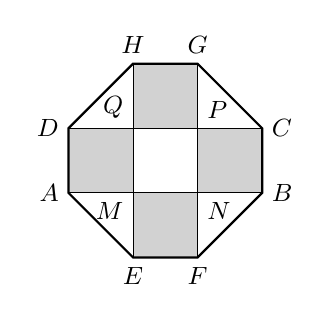
\begin{tikzpicture}[scale=0.82, every node/.style={font=\small}]
  \fill[gray!35] (-1.5,-0.5) rectangle (1.5,0.5);
  \fill[gray!35] (-0.5,-1.5) rectangle (0.5,1.5);
  % 中心正方形 MNPQ 原卷不涂阴影，照原卷留白：
  \fill[white] (-0.5,-0.5) rectangle (0.5,0.5);
  \draw[thick] (-1.5,0.5)--(-0.5,1.5)--(0.5,1.5)--(1.5,0.5)--(1.5,-0.5)--(0.5,-1.5)--(-0.5,-1.5)--(-1.5,-0.5)--cycle;
  \draw (-1.5,-0.5) rectangle (1.5,0.5);
  \draw (-0.5,-1.5) rectangle (0.5,1.5);
  \node[left] at (-1.5,0.5) {$D$};
  \node[left] at (-1.5,-0.5) {$A$};
  \node[right] at (1.5,0.5) {$C$};
  \node[right] at (1.5,-0.5) {$B$};
  \node[above] at (-0.5,1.5) {$H$};
  \node[above] at (0.5,1.5) {$G$};
  \node[below] at (-0.5,-1.5) {$E$};
  \node[below] at (0.5,-1.5) {$F$};
  \node[below left] at (-0.5,-0.5) {$M$};
  \node[below right] at (0.5,-0.5) {$N$};
  \node[above right] at (0.5,0.5) {$P$};
  \node[above left] at (-0.5,0.5) {$Q$};
\end{tikzpicture}
\end{center}

\begin{enumerate}[label=(\arabic*)]
\item 设 $DQ$ 长为 $y$（单位：m），用 $x$ 表示 $y$，并求出 $x$ 的取值范围；
\item $AD$ 取何值时可使总造价最低，并求出最低造价.
\end{enumerate}

\ifanswer
\solbegin
\stepm{(1)}{设 $AD=x\text{m}$（$x>0$），$DQ=y\text{m}$（$y>0$），}
\step{因为十字形区域总面积为 $200\text{m}^2$，所以 $4xy+x^2=200$，}
\step{解得 $y=\dfrac{200-x^2}{4x}=\dfrac{50}{x}-\dfrac{x}{4}$，}
\step{因为 $x>0$，$y>0$，所以 $y=\dfrac{200-x^2}{4x}>0$，解得 $0<x<10\sqrt2$，}
\step{所以 $y=\dfrac{50}{x}-\dfrac{x}{4}$，$0<x<10\sqrt2$；}
\stepm{(2)}{中心正方形 $MNPQ$ 区域，造价为 $2100$ 元$/\text{m}^2$，}
\step{中心正方形 $MNPQ$ 面积为 $S_1=x^2$，造价为 $W_1=2100\times S_1=2100x^2$；}
\step{周围四个矩形区域（图中阴影部分）铺设透水地砖，造价为 $105$ 元$/\text{m}^2$，}
\step{四个矩形的总面积为 $S_2=4xy=4x\left(\dfrac{50}{x}-\dfrac{x}{4}\right)=200-x^2$，}
\step{造价为 $W_2=105\times S_2=105(200-x^2)=21000-105x^2$；}
\step{四个三角形区域种植耐旱固碳植物，助力碳中和，造价为 $40$ 元$/\text{m}^2$，}
\step{四个三角形的总面积为 $S_3=4\times\dfrac12y^2=2\left(\dfrac{50}{x}-\dfrac{x}{4}\right)^2
=\dfrac{5000}{x^2}-50+\dfrac{x^2}{8}$，}
\step{造价为 $W_3=40\times S_3=40\left(\dfrac{5000}{x^2}-50+\dfrac{x^2}{8}\right)
=\dfrac{200000}{x^2}-2000+5x^2$；}
\step{设总造价为 $W$（单位：元），}
\step{则总造价为 $W=W_1+W_2+W_3$}
\step{$=2100x^2+21000-105x^2+\dfrac{200000}{x^2}-2000+5x^2$}
\step{$=2000x^2+\dfrac{200000}{x^2}+19000$，}
\step{又 $2000x^2+\dfrac{200000}{x^2}\geqslant2\sqrt{2000x^2\times\dfrac{200000}{x^2}}=2\times20000=40000$，}
\step{当且仅当 $2000x^2=\dfrac{200000}{x^2}$，即 $x=\sqrt{10}$（在 $x$ 的范围内）时取等号，}
\step{所以 $W=2000x^2+\dfrac{200000}{x^2}+19000\geqslant59000$，当 $x=\sqrt{10}$ 时取等号，}
\step{故当 $AD$ 的长为 $\sqrt{10}$ 时，总造价最低，为 $59000$ 元.}
\solend

\fi

\ansspace[8]

\item 对于实数 $a$、$b$、$c$，若 $|a-c|<|b-c|$，则称 $a$ 比 $b$ 更接近于 $c$. 现已知 $p$、$q$ 都是正有理数.

\begin{enumerate}[label=(\arabic*)]
\item 证明：$\sqrt3$ 必在 $\dfrac pq$ 和 $\dfrac{p+3q}{p+q}$ 之间；
\item 试问 $\dfrac pq$ 和 $\dfrac{p+3q}{p+q}$ 这两个数，哪一个更接近于 $\sqrt3$？说明你的理由；
\item 请你再写出一个有理数，使得它的值比 $\dfrac pq$ 和 $\dfrac{p+3q}{p+q}$ 的值更接近于 $\sqrt3$，并说明你的理由.
\end{enumerate}

\ifanswer
\solbegin
\stepm{(1)}{设 $a=\dfrac pq$（$a$ 为正有理数），则需证 $\sqrt3$ 在 $a$ 和 $\dfrac{a+3}{a+1}$（即 $\dfrac{p+3q}{p+q}$）之间.}
\step{当 $a>\sqrt3$ 时，计算 $a-\dfrac{a+3}{a+1}$ 得 $a-\dfrac{a+3}{a+1}=\dfrac{a(a+1)-(a+3)}{a+1}=\dfrac{a^2-3}{a+1}$，}
\step{$a>\sqrt3$，则 $a^2-3>0$，故 $a>\dfrac{a+3}{a+1}$；}
\step{再计算 $\dfrac{a+3}{a+1}-\sqrt3$ 得 $\dfrac{a+3}{a+1}-\sqrt3=\dfrac{(1-\sqrt3)(a-\sqrt3)}{a+1}$，}
\step{$1-\sqrt3<0$，$a-\sqrt3>0$，$a+1>0$，}
\step{故 $\dfrac{a+3}{a+1}-\sqrt3<0$，即 $\dfrac{a+3}{a+1}<\sqrt3$，从而 $\dfrac{a+3}{a+1}<\sqrt3<a$；}
\step{当 $a<\sqrt3$ 时，同理可得 $a<\dfrac{a+3}{a+1}$ 且 $\dfrac{a+3}{a+1}>\sqrt3$，即 $a<\sqrt3<\dfrac{a+3}{a+1}$，}
\step{综上，$\sqrt3$ 必在 $\dfrac pq$ 和 $\dfrac{p+3q}{p+q}$ 之间；}
\stepm{(2)}{设 $a=\dfrac pq$，$b=\dfrac{p+3q}{p+q}=\dfrac{a+3}{a+1}$，比较 $|a-\sqrt3|$ 与 $|b-\sqrt3|$，}
\step{由（1）得 $(a-\sqrt3)(b-\sqrt3)<0$，}
\step{$\dfrac{|b-\sqrt3|}{|a-\sqrt3|}
=\left|\dfrac{b-\sqrt3}{a-\sqrt3}\right|
=\dfrac{\left|\dfrac{(1-\sqrt3)(a-\sqrt3)}{a+1}\right|}{|a-\sqrt3|}
=\dfrac{\sqrt3-1}{a+1}$，}
\step{$a>0$，$a+1>1$，$\sqrt3-1<1$，故 $\dfrac{\sqrt3-1}{a+1}<1$，即 $|b-\sqrt3|<|a-\sqrt3|$，}
\step{即 $\dfrac{p+3q}{p+q}$ 比 $\dfrac pq$ 更接近于 $\sqrt3$；}
\stepm{(3)}{$\dfrac{2p+3q}{p+2q}$，理由：}
\step{设 $b=\dfrac{p+3q}{p+q}$，新数 $c=\dfrac{b+3}{b+1}=\dfrac{2p+3q}{p+2q}$，}
\step{由（1）得 $(b-\sqrt3)(c-\sqrt3)<0$，}
\step{$c-\sqrt3=\dfrac{b+3}{b+1}-\sqrt3=\dfrac{(1-\sqrt3)(b-\sqrt3)}{b+1}$，}
\step{则 $\dfrac{|c-\sqrt3|}{|b-\sqrt3|}
=\left|\dfrac{c-\sqrt3}{b-\sqrt3}\right|
=\dfrac{\left|\dfrac{(1-\sqrt3)(b-\sqrt3)}{b+1}\right|}{|b-\sqrt3|}
=\dfrac{\sqrt3-1}{b+1}$，}
\step{$b>0$，$b+1>1$，$0<\sqrt3-1<1$，故 $\dfrac{\sqrt3-1}{b+1}<1$，即 $|c-\sqrt3|<|b-\sqrt3|$，}
\step{即 $\dfrac{2p+3q}{p+2q}$ 比 $\dfrac{p+3q}{p+q}$ 更接近于 $\sqrt3$，故 $c$ 更接近 $\sqrt3$.}
\solend

\fi

\ansspace*[10]

\end{enumerate}

\end{document}
"
% 紧凑版：xelatex "\def\iscompact{1}% 高一45_交附闵行_国庆作业2.tex
%   —— 高一上数学“2026-2027 年交附闵行高一上国庆作业 2”（试卷版/答案版）
% 试卷版：xelatex 高一45_交附闵行_国庆作业2.tex
% 答案版：xelatex "\def\isanswer{1}\input{高一45_交附闵行_国庆作业2.tex}"
% 紧凑版：xelatex "\def\iscompact{1}\input{高一45_交附闵行_国庆作业2.tex}"
%
% 原始材料是微信公众号图文（公众号“魔都数学加油站”，作者“破晓”，2026-10-02 17:56 发布，
% 连载“27学年高一45”，原文标题“27学年高一45——2026-2027年上海市交附闵行高一上国庆作业2”，
% https://mp.weixin.qq.com/s/1xdCtzH-3Il0jJrz3saiPA），正文为 10 张 PNG 页。
% 第 01—06、09 页为 4762×6735；第 07、08、10 页为 2560×3620（同一篇各页原图分辨率不一致）。
% 原文本身是一份讲评版：第 3—21 题均照原卷保留题目与题下解析；第 13 题原卷把答案 C 印在括号中。
% 题目、选项、答案与解析均照原卷录入，未改内容；卷面的粉色斜水印及页脚不录入。
%
% 卷首标题：原卷印作“2026-2027 年交附闵行高一上国庆作业 2”（公众号标题里的“上海市”
% 三字卷面标题行没有，本稿照卷面），年份区间按全稿惯例排 en dash，前缀照原卷保留“年”。
%
% 与原卷的排版差异：
%   ① 原卷印有“一、填空题”“二、选择题”“三、解答题”三节标题，本稿照原卷分节，
%      只把标题改排成全稿统一的“大节标题”样式；
%   ② 第 13 题原卷在题干括号内直接印答案 C，本稿按全稿样式将括号留空、答案移入答案版的 \ans{}；
%   ③ 原卷填空横线及选择题答案括号均按全稿样式排版，填空横线统一用 \blankline[4.4em]；
%   ④ 原卷第 20 题配有十字形广场示意图，本稿在源码中用 TikZ 重绘，图中区域、边界及点名照原卷。
%   ⑤ 原卷未印副标题，本稿按本卷实际涉及的知识模块补出“集合与常用逻辑用语、不等式”。
%
% 原卷存疑/错误（均照抄原卷、未改，见对应题目处上方注释）：
%   ① 第 11 题解析原卷印"所以 p=3+9=12，又 12,15∉A，所以 12,15∉B"，与 A∪\overline{B} 的条件
%      及后文 B 的根为 6、9 均一致，无矛盾，本稿照录（早前记录的"∈B／前后矛盾"系本稿误读）；
%   ② 第 15 题题干与解析均按原卷印 ac<0，解析"因为 a<b<c，且 ac<0，所以 a<0，c>0"与题设一致，
%      无矛盾（早前记录的"abc<0／解析冲突"系本稿误读题干所致）；本稿照录原卷答案与解析。
%   ③ 第 20 题原卷各数（造价 2100 元/m^2、W_1=2100x^2、合并式 2000x^2+200000/x^2+19000、
%      末句 59000 元）经复核自洽，无矛盾（早前记录的"W_1=200x^2／末句 5900 元"系本稿误录）；本稿照录。
%   ④ 第 18(2) 题 a=-1 时 A=B=(-1,1)，不满足“B 是 A 的真子集”，故原解析给出的 a≤-1 应为 a<-1；
%   ⑤ 第 19(2) 题原卷用"{c|0<c<1}∩{c|c<-2√3/3 或 c>2√3/3}=∅"论证"不等式①、②中至多有一个恒成立"，
%      论证成立（早前记录的"区间并集留有间隙"系本稿误录解析所致）；本稿照录原卷。
%
\documentclass[a4paper,11pt]{article}
\usepackage{common}

\begin{document}

\examtitlest[3]{2026--2027 年交附闵行高一上国庆作业 2}{集合与常用逻辑用语、不等式}

\bigsec{一、填空题}

\begin{enumerate}
\setcounter{enumi}{2}

\item 满足 $A\cup\{-1,1\}=\{-1,0,1\}$ 的集合 $A$ 共有 \blankline[4.4em] 个.

\ifanswer
\solbegin
\step{集合可能为 $\{0\}$、$\{0,1\}$、$\{0,-1\}$、$\{0,1,-1\}$，共有 $4$ 个.}
\solend

\fi

\item 设 $x\in\R$，则“$x+\dfrac1x>2$”是“$x\neq1$”的 \blankline[4.4em] 条件.

\ifanswer
\solbegin
\step{$x+\dfrac1x>2\Longleftrightarrow x>0$ 且 $x\neq1$，故为充分不必要条件.}
\solend

\fi

\item 已知集合 $A=\{x\mid|x-1|<a\}$，$B=\{-4,3\}$，若 $A\cap B=\varnothing$，则 $a$ 的最大值为 \blankline[4.4em].

\ifanswer
\solbegin
\step{$A=\{x\mid -a<x-1<a\}=\{x\mid1-a<x<1+a\}$，$B=\{-4,3\}$，且 $A\cap B=\varnothing$，}
\step{$A=\varnothing$ 时，$1-a\geqslant1+a$，解得 $a\leqslant0$，满足 $A\cap B=\varnothing$；}
\step{若 $-4\in A$，则 $1-a<-4<1+a$，解得 $a>5$；}
\step{若 $3\in A$，则 $1-a<3<1+a$，解得 $a>2$，}
\step{因为 $A\cap B=\varnothing$，所以 $-4\notin A$ 且 $3\notin A$，所以 $a\leqslant5$ 且 $a\leqslant2$，所以 $a\leqslant2$，}
\step{综上，$a$ 的最大值为 $2$.}
\solend

\fi

\item 设 $x\in\R$，方程 $|x-1|+|2x-1|=|3x-2|$ 的解集为 \blankline[4.4em].

\ifanswer
\solbegin
\step{因为 $|x-1|+|2x-1|\geqslant|(x-1)+(2x-1)|=|3x-2|$，}
\step{当且仅当 $(x-1)(2x-1)\geqslant0$，解得 $x\leqslant\dfrac12$ 或 $x\geqslant1$，}
\step{故方程 $|x-1|+|2x-1|=|3x-2|$ 的解集为 $\left(-\infty,\dfrac12\right]\cup[1,+\infty)$.}
\solend

\fi

\item 已知 $a$、$b\in\R$，且 $3a+2b=1$，则 $8^a+4^b$ 最小值为 \blankline[4.4em].

\ifanswer
\solbegin
% 注：原卷本行与上行均作“$8^a+4^b$ 最小值为”，“最小值”前无“的”，原卷如此，照录未改。
\step{因为 $3a+2b=1$，所以 $8^a+4^b=2^{3a}+2^{2b}\geqslant2\sqrt{2^{3a+2b}}=2\sqrt2$，}
\step{当且仅当 $3a=2b$ 时取等号，故 $8^a+4^b$ 最小值为 $2\sqrt2$.}
\solend

\fi

\item 已知 $a>0$，$b>0$，且 $a+2b+ab=30$，则 $2a+b$ 的最小值为 \blankline[4.4em].

\ifanswer
\solbegin
\step{由 $a+2b+ab=30$，得 $(a+2)(b+1)=32$.}
\step{因为 $a>0$，$b>0$，所以 $a+2>0$，$b+1>0$，}
\step{所以 $2a+b=2(a+2)+(b+1)-5\geqslant2\sqrt{2\times32}-5=11$，}
\step{当且仅当 $2(a+2)=(b+1)$，即 $a=2$，$b=7$ 时取等号，}
\step{所以 $2a+b$ 的最小值为 $11$.}
\solend

\fi

\item 已知 $A=\{x\mid x^2+px+1=0\}$，$M=\{x\mid x>0\}$，若 $A\cap M=\varnothing$，则实数 $p$ 的取值范围为 \blankline[4.4em].

\ifanswer
\solbegin
\step{①当 $A=\varnothing$ 时，$\Delta=p^2-4<0$，所以 $-2<p<2$，此时满足 $A\cap M=\varnothing$；}
\step{②当 $A\neq\varnothing$ 时，$\Delta=p^2-4\geqslant0$，$p\geqslant2$ 或 $p\leqslant-2$，}
\step{因为 $M=\{x\mid x>0\}$，$A\cap M=\varnothing$，由韦达定理得 $\begin{cases}-p\leqslant0\\1>0\end{cases}$，解得 $p\geqslant0$，}
\step{所以 $p\geqslant2$，}
\step{由①②综合得 $p>-2$，故实数 $p$ 的取值范围为 $(-2,+\infty)$.}
\solend

\fi

\item 已知集合 $A=[t,t+1]\cup[t+3,t+6]$，其中 $t>0$. 若存在正数 $\lambda$，使得对任意 $a\in A$，都有 $\dfrac{\lambda}{a}\in A$，则 $t$ 的取值集合为 \blankline[4.4em].

\ifanswer
\solbegin
\step{因为 $0\notin A$，$t>0$，所以 $a\in[t,t+1]\cup[t+3,t+6]$，}
\step{则 $\dfrac1a\in\left[\dfrac1{t+6},\dfrac1{t+3}\right]\cup\left[\dfrac1{t+1},\dfrac1t\right]$，}
\step{又因为 $\lambda>0$，所以 $\dfrac{\lambda}{a}\in\left[\dfrac{\lambda}{t+6},\dfrac{\lambda}{t+3}\right]\cup\left[\dfrac{\lambda}{t+1},\dfrac{\lambda}{t}\right]$，}
\step{因为 $\dfrac{\lambda}{a}\in A$，所以 $\begin{cases}\dfrac{\lambda}{t+6}\geqslant t\\[3pt]\dfrac{\lambda}{t+3}\leqslant t+1\end{cases}$ 且 $\begin{cases}\dfrac{\lambda}{t+1}\geqslant t+3\\[3pt]\dfrac{\lambda}{t}\leqslant t+6\end{cases}$，}
% 注：原卷本行两个不等式组印作“$t(t+6)\leqslant\lambda\leqslant t(t+6)$”与
%     “$(t+1)(t+3)\leqslant\lambda\leqslant(t+1)(t+3)$”（两侧同式），与上行两式推导不合，系原卷笔误；
%     原卷如此，照录未改。
\step{得 $\begin{cases}t(t+6)\leqslant\lambda\leqslant t(t+6)\\[3pt](t+1)(t+3)\leqslant\lambda\leqslant(t+1)(t+3)\end{cases}$，所以 $\lambda=t(t+6)=(t+1)(t+3)$，}
\step{解得 $t=\dfrac32$，取值集合为 $\left\{\dfrac32\right\}$.}
\solend

\fi

\item 已知全集 $U=\{x\mid x=3n,1\leqslant n\leqslant5\ \text{且}\ n\in\N\}$，$A=\{x\mid x^2-px+27=0,p\in\N\}$，
$B=\{x\mid x^2-15x+q=0,q\in\N\}$，且 $A\cup\overline{B}=\{3,9,12,15\}$，则 $p+q$ 的值为 \blankline[4.4em].

\ifanswer
\solbegin
\step{因为全集 $U=\{3,6,9,12,15\}$，$A\cup\overline{B}=\{3,9,12,15\}$，}
\step{所以 $3$、$9$、$12$、$15$ 中可能有两个属于 $A$，}
\step{因为 $A$ 中的方程 $x^2-px+27=0$ 中，两根之积 $x_1x_2=27$，所以 $3$、$9\in A$，}
\step{所以 $p=3+9=12$，又 $12$、$15\notin A$，所以 $12$、$15\notin B$，}
\step{因为 $B$ 中的方程 $x^2-15x+q=0$ 中，两根之和 $x_3+x_4=15$，所以 $6$、$9\in B$，}
\step{则 $q=6\times9=54$，所以 $p+q=66$.}
\solend

\fi

\item 若关于 $x$ 的不等式 $|x-2k|+|x-3k|<4k$ 共有 $2025$ 个整数解，则实数 $k$ 的取值范围为 \blankline[4.4em].

\ifanswer
\solbegin
\step{显然 $k>0$，由 $|x-2k|+|x-3k|<4k$，得 $\dfrac{k}{2}<x<\dfrac{9k}{2}$，}
\step{因为该不等式共有 $2025$ 个整数解，所以 $2024<\dfrac{9k}{2}-\dfrac{k}{2}\leqslant2026$，}
\step{解得 $506<k\leqslant506.5$，}
\step{由 $\dfrac{k}{2}\in(253,253.25]$，得这 $2025$ 个整数解只能为 $254,255,256,\cdots,2278$，}
\step{所以 $2278<\dfrac{9k}{2}\leqslant2279$，解得 $506\dfrac29<k\leqslant506\dfrac49$，结合 $506<k\leqslant506.5$，}
\step{得 $k$ 的取值范围是 $\left(506\dfrac29,506\dfrac49\right]$.}
\solend

\fi

\end{enumerate}

\bigsec{二、选择题}

\begin{enumerate}
\setcounter{enumi}{12}

\item 已知 $a,b\in\R$，且 $ab\neq0$，则下列结论恒成立的是\mbox{（\quad）}

\keepwithprev
A. $a+b\geqslant2\sqrt{ab}$\qquad
B. $\left(\dfrac{a+b}{2}\right)^2>ab$\qquad
C. $\left|\dfrac ab+\dfrac ba\right|\geqslant2$\qquad
D. $a^2+b^2>2ab$

\ans{$C$}

\item 如果 $a^{2025}+b^{2025}=0$，那么一定有\mbox{（\quad）}

\keepwithprev
A. $(|a|+|b|)^{2025}=0$\qquad
B. $(a-b)^{2025}=0$\qquad
C. $(a\cdot b)^{2025}=0$\qquad
D. $(a+b)^{2025}=0$

\ans{$D$}

\ifanswer
\solbegin
\step{由 $a^{2025}+b^{2025}=0$，得 $a^{2025}=-b^{2025}=(-b)^{2025}$，则 $\left(a^{2025}\right)^{\frac{1}{2025}}=\left[(-b)^{2025}\right]^{\frac{1}{2025}}$，}
\step{即 $a=-b$，即 $a+b=0$，故 $(a+b)^{2025}=0$，故 D 符合题意；}
\step{对于 A，若取 $a=1$，$b=-1$，则 $(|a|+|b|)^{2025}=2^{2025}\neq0$，故 A 不合题意；}
\step{对于 B，若取 $a=1$，$b=-1$，则 $(a-b)^{2025}=2^{2025}\neq0$，故 B 不合题意；}
\step{对于 C，若取 $a=1$，$b=-1$，则 $(a\cdot b)^{2025}=(-1)^{2025}=-1\neq0$，故 C 不合题意；}
\step{故选 D.}
\solend

\fi

\item 已知 $a$、$b$、$c$ 满足 $a<b<c$，且 $ac<0$，那么下列各式中一定成立的是\mbox{（\quad）}

\keepwithprev
A. $\dfrac1a>\dfrac1c$\qquad
B. $ab^2<cb^2$\qquad
C. $ac<bc$\qquad
D. $a+c>2b$

\ans{$C$}

\ifanswer
\solbegin
\step{因为 $a<b<c$，且 $ac<0$，所以 $a<0$，$c>0$，}
\step{对于 A，$\dfrac1a<0<\dfrac1c$，故 A 错误；}
\step{对于 B，当 $b=0$ 时，$ab^2=cb^2$，故 B 错误；}
\step{对于 C，$ac<bc$ 可化为 $(a-b)c<0$，因为 $a<b$，所以 $a-b<0$，}
\step{又因为 $c>0$，所以 $(a-b)c<0$，所以 C 正确；}
\step{对于 D，设 $a=-2$，$b=0$，$c=1$，则 $a+c<2b$，故 D 错误.}
\step{故选 C.}
\solend

\fi

\item 对于 $a\in\R$，设集合 $A=\left\{x\mid\dfrac{(x^2-6x+a)(x-1)}{x+a}=0\right\}$，记 $A$ 的所有元素之和为 $S(a)$，
所有元素之积为 $T(a)$，则下列说法中，正确的是\mbox{（\quad）}

\keepwithprev
A. 不存在实数 $a$，使得 $S(a)=6$\qquad
B. 存在实数 $a$，使得 $T(a)=9$

C. 存在无数实数 $a$，使得 $S(a)=7$\qquad
D. 若 $T(a)=3$，则 $a=3$

\ans{$C$}

\ifanswer
\solbegin
\step{要使 $\dfrac{(x^2-6x+a)(x-1)}{x+a}=0$，只需 $(x^2-6x+a)(x-1)=0$ 且 $x+a\neq0$，}
\step{由 $(x^2-6x+a)(x-1)=0$ 得 $x^2-6x+a=0$ 或 $x-1=0$，}
\step{对于一元二次方程 $x^2-6x+a=0$，其判别式 $\Delta=36-4a$，}
\step{当 $\Delta=0$，即 $a=9$ 时，集合 $A=\{1,3\}$，$S(a)=4$，$T(a)=3$；}
\step{当 $\Delta<0$，即 $a>9$ 时，集合 $A=\{1\}$，$S(a)=T(a)=1$；}
\step{当 $\Delta>0$，即 $a<9$ 时，一元二次方程 $x^2-6x+a=0$ 的解为 $x=3\pm\sqrt{9-a}$，}
\step{①当 $a=0$ 时，$x\neq0$，则集合 $A=\{1,6\}$，则 $S(a)=7$，$T(a)=6$，}
\step{②当 $a=-7$ 时，$x\neq7$，则集合 $A=\{-1,1\}$，则 $S(a)=0$，$T(a)=-1$，}
% 注：下一行集合 A 原卷印作 {-1,1}（按 a=-1 代入 x^2-6x-1=0 应得 3±√10，原卷如此，照录未改）。
\step{③当 $a=-1$ 时，$x\neq1$，则集合 $A=\{-1,1\}$，则 $S(a)=6$，$T(a)=-1$，}
\step{④当 $a=5$ 时，$x\neq-5$，则集合 $A=\{1,5\}$，则 $S(a)=6$，$T(a)=5$，}
\step{⑤当 $a\neq5,0,-1,-7$ 时，集合 $A=\{1,3-\sqrt{9-a},3+\sqrt{9-a}\}$，}
\step{则 $S(a)=7$，$T(a)=a$.}
\step{选项 A，当 $a=5$ 时，$S(a)=6$，所以 A 错误；}
\step{选项 B，$T(a)$ 的可能值为 $-1,1,3,5,6,a$（$a<9$），无 $T(a)=9$，所以 B 错误；}
\step{选项 C，当 $a<9$，且 $a\neq5,-1,-7$ 时，$S(a)=7$，有无数个 $a$ 满足，所以 C 正确；}
\step{选项 D，当 $T(a)=3$ 时，有 $a=3$ 和 $a=9$ 满足，所以 D 错误.}
\step{故选 C.}
\solend

\fi

\end{enumerate}

\bigsec{三、解答题}

\begin{enumerate}
\setcounter{enumi}{16}

\item 已知 $a\in\R$，关于 $x$ 的不等式 $|x+1|+|x-1|>a^2-5a+4$.

\begin{enumerate}[label=(\arabic*)]
\item 当 $a=0$ 时，求不等式的解集；
\item 若不等式的解集为 $\R$，求 $a$ 的取值范围.
\end{enumerate}

\ifanswer
\solbegin
\stepm{(1)}{当 $a=0$ 时，不等式为 $|x+1|+|x-1|>4$，}
\step{又 $|x+1|+|x-1|=\begin{cases}2x,&x\geqslant1\\2,&-1<x<1\\-2x,&x\leqslant-1\end{cases}$，}
\step{则 $|x+1|+|x-1|>4$ 的解为 $x>2$ 或 $x<-2$，}
\step{即不等式的解集为 $(-\infty,-2)\cup(2,+\infty)$；}
\stepm{(2)}{不等式 $|x+1|+|x-1|>a^2-5a+4$ 的解集为 $\R$，}
\step{则 $(|x+1|+|x-1|)_{\min}>a^2-5a+4$，}
\step{又 $(|x+1|+|x-1|)_{\min}=2$，当且仅当 $-1\leqslant x\leqslant1$ 时取得，即 $a^2-5a+4<2$，}
\step{即 $a^2-5a+2<0$，即 $\dfrac{5-\sqrt{17}}2<a<\dfrac{5+\sqrt{17}}2$，}
\step{即 $a$ 的取值范围为 $\left(\dfrac{5-\sqrt{17}}2,\dfrac{5+\sqrt{17}}2\right)$.}
\solend

\fi

\ansspace[6]

\item 已知集合 $A=\{x\mid(x-a)(x-a^2)<0\}$，集合 $B=\left\{x\mid\dfrac{2x}{x-1}<1\right\}$，命题 $p:x\in A$，命题 $q:x\in B$.

\begin{enumerate}[label=(\arabic*)]
\item 当实数 $a$ 为何值时，$A=B$；
\item 若 $q$ 是 $p$ 的充分不必要条件，求实数 $a$ 的取值范围.
\end{enumerate}

\ifanswer
\solbegin
\stepm{(1)}{由 $\dfrac{2x}{x-1}<1$ 得 $\dfrac{2x}{x-1}-1=\dfrac{x+1}{x-1}<0$，解得 $-1<x<1$，即 $B=\{x\mid-1<x<1\}$，}
\step{因为 $A=\{x\mid(x-a)(x-a^2)<0\}$，$A=B$，所以 $\begin{cases}a=-1\\a^2=1\end{cases}$，解得 $a=-1$；}
\stepm{(2)}{若 $q$ 是 $p$ 的充分不必要条件，则 $B\subset A$，}
\step{当 $a^2=a$，即 $a=0$ 或 $a=1$ 时，$A=\varnothing$，显然不符合题意；}
\step{当 $a^2>a$，即 $a>1$ 或 $a<0$ 时，$A=(a,a^2)$，则 $\begin{cases}a\leqslant-1\\a^2\geqslant1\\a>1\ \text{或}\ a<0\end{cases}$，}
% 注：a=-1 时 A=(-1,1)=B，不是 B 的真子集；原解析用 B⊂A 但答案含 -1，照录。
\step{前两等号不能同时取得，解得 $a\leqslant-1$；}
\step{当 $a^2<a$，即 $0<a<1$ 时，$A=(a^2,a)$，显然不符合题意，}
\step{故 $a$ 的范围为 $\{a\mid a\leqslant-1\}$.}
\solend

\fi

\ansspace[6]

\item 已知不等式① $x^2+2cx+c>0$，② $x^2+cx+c^2-1>0$，其中 $c$ 是实数.

\begin{enumerate}[label=(\arabic*)]
\item 若 $1$ 是不等式②的一个解，求实数 $c$ 的取值范围；
\item 证明：不等式①、②中至多有一个恒成立.
\end{enumerate}

\ifanswer
\solbegin
\stepm{(1)}{已知不等式① $x^2+2cx+c>0$，② $x^2+cx+c^2-1>0$，}
\step{又 $1$ 是不等式②的一个解，则 $1+c+c^2-1>0$，}
\step{则 $c^2+c>0$，则 $c<-1$ 或 $c>0$，则 $c$ 的取值范围为 $(-\infty,-1)\cup(0,+\infty)$；}
\stepm{(2)}{若不等式①恒成立，则 $\Delta=4c^2-4c<0$，则 $0<c<1$，}
\step{若不等式②恒成立，则 $\Delta=c^2-4(c^2-1)=4-3c^2<0$，}
\step{则 $c<-\dfrac{2\sqrt3}{3}$ 或 $c>\dfrac{2\sqrt3}{3}$，}
\step{又 $\{c\mid 0<c<1\}\cap\left\{c\mid c<-\dfrac{2\sqrt3}{3}\ \text{或}\ c>\dfrac{2\sqrt3}{3}\right\}=\varnothing$，}
\step{则不存在实数 $c$ 使得不等式①、②同时恒成立，}
\step{则不等式①、②中至多有一个恒成立.}
\solend

\fi

\ansspace[6]

\item 为践行“科技强国”战略，某社区计划建造一座融合智慧节能技术的八边形休闲广场，其中两个相同的矩形 $ABCD$ 和 $EFGH$ 构成的十字形区域总面积为 $200\text{m}^2$. 中心正方形 $MNPQ$ 区域将安装国产太阳能光伏板（兼具休憩遮阳功能），造价为 $2100$ 元$/\text{m}^2$；周围四个矩形区域（图中阴影部分）铺设透水地砖，造价为 $105$ 元$/\text{m}^2$；再在四个三角形区域种植耐旱固碳植物，助力碳中和，造价为 $40$ 元$/\text{m}^2$. 设总造价为 $W$（单位：元），$AD=x$（单位：m）.

\begin{center}
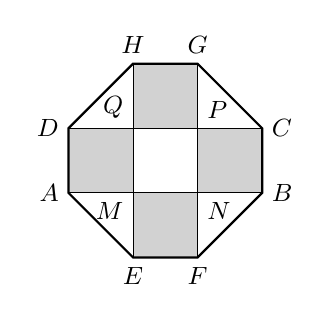
\begin{tikzpicture}[scale=0.82, every node/.style={font=\small}]
  \fill[gray!35] (-1.5,-0.5) rectangle (1.5,0.5);
  \fill[gray!35] (-0.5,-1.5) rectangle (0.5,1.5);
  % 中心正方形 MNPQ 原卷不涂阴影，照原卷留白：
  \fill[white] (-0.5,-0.5) rectangle (0.5,0.5);
  \draw[thick] (-1.5,0.5)--(-0.5,1.5)--(0.5,1.5)--(1.5,0.5)--(1.5,-0.5)--(0.5,-1.5)--(-0.5,-1.5)--(-1.5,-0.5)--cycle;
  \draw (-1.5,-0.5) rectangle (1.5,0.5);
  \draw (-0.5,-1.5) rectangle (0.5,1.5);
  \node[left] at (-1.5,0.5) {$D$};
  \node[left] at (-1.5,-0.5) {$A$};
  \node[right] at (1.5,0.5) {$C$};
  \node[right] at (1.5,-0.5) {$B$};
  \node[above] at (-0.5,1.5) {$H$};
  \node[above] at (0.5,1.5) {$G$};
  \node[below] at (-0.5,-1.5) {$E$};
  \node[below] at (0.5,-1.5) {$F$};
  \node[below left] at (-0.5,-0.5) {$M$};
  \node[below right] at (0.5,-0.5) {$N$};
  \node[above right] at (0.5,0.5) {$P$};
  \node[above left] at (-0.5,0.5) {$Q$};
\end{tikzpicture}
\end{center}

\begin{enumerate}[label=(\arabic*)]
\item 设 $DQ$ 长为 $y$（单位：m），用 $x$ 表示 $y$，并求出 $x$ 的取值范围；
\item $AD$ 取何值时可使总造价最低，并求出最低造价.
\end{enumerate}

\ifanswer
\solbegin
\stepm{(1)}{设 $AD=x\text{m}$（$x>0$），$DQ=y\text{m}$（$y>0$），}
\step{因为十字形区域总面积为 $200\text{m}^2$，所以 $4xy+x^2=200$，}
\step{解得 $y=\dfrac{200-x^2}{4x}=\dfrac{50}{x}-\dfrac{x}{4}$，}
\step{因为 $x>0$，$y>0$，所以 $y=\dfrac{200-x^2}{4x}>0$，解得 $0<x<10\sqrt2$，}
\step{所以 $y=\dfrac{50}{x}-\dfrac{x}{4}$，$0<x<10\sqrt2$；}
\stepm{(2)}{中心正方形 $MNPQ$ 区域，造价为 $2100$ 元$/\text{m}^2$，}
\step{中心正方形 $MNPQ$ 面积为 $S_1=x^2$，造价为 $W_1=2100\times S_1=2100x^2$；}
\step{周围四个矩形区域（图中阴影部分）铺设透水地砖，造价为 $105$ 元$/\text{m}^2$，}
\step{四个矩形的总面积为 $S_2=4xy=4x\left(\dfrac{50}{x}-\dfrac{x}{4}\right)=200-x^2$，}
\step{造价为 $W_2=105\times S_2=105(200-x^2)=21000-105x^2$；}
\step{四个三角形区域种植耐旱固碳植物，助力碳中和，造价为 $40$ 元$/\text{m}^2$，}
\step{四个三角形的总面积为 $S_3=4\times\dfrac12y^2=2\left(\dfrac{50}{x}-\dfrac{x}{4}\right)^2
=\dfrac{5000}{x^2}-50+\dfrac{x^2}{8}$，}
\step{造价为 $W_3=40\times S_3=40\left(\dfrac{5000}{x^2}-50+\dfrac{x^2}{8}\right)
=\dfrac{200000}{x^2}-2000+5x^2$；}
\step{设总造价为 $W$（单位：元），}
\step{则总造价为 $W=W_1+W_2+W_3$}
\step{$=2100x^2+21000-105x^2+\dfrac{200000}{x^2}-2000+5x^2$}
\step{$=2000x^2+\dfrac{200000}{x^2}+19000$，}
\step{又 $2000x^2+\dfrac{200000}{x^2}\geqslant2\sqrt{2000x^2\times\dfrac{200000}{x^2}}=2\times20000=40000$，}
\step{当且仅当 $2000x^2=\dfrac{200000}{x^2}$，即 $x=\sqrt{10}$（在 $x$ 的范围内）时取等号，}
\step{所以 $W=2000x^2+\dfrac{200000}{x^2}+19000\geqslant59000$，当 $x=\sqrt{10}$ 时取等号，}
\step{故当 $AD$ 的长为 $\sqrt{10}$ 时，总造价最低，为 $59000$ 元.}
\solend

\fi

\ansspace[8]

\item 对于实数 $a$、$b$、$c$，若 $|a-c|<|b-c|$，则称 $a$ 比 $b$ 更接近于 $c$. 现已知 $p$、$q$ 都是正有理数.

\begin{enumerate}[label=(\arabic*)]
\item 证明：$\sqrt3$ 必在 $\dfrac pq$ 和 $\dfrac{p+3q}{p+q}$ 之间；
\item 试问 $\dfrac pq$ 和 $\dfrac{p+3q}{p+q}$ 这两个数，哪一个更接近于 $\sqrt3$？说明你的理由；
\item 请你再写出一个有理数，使得它的值比 $\dfrac pq$ 和 $\dfrac{p+3q}{p+q}$ 的值更接近于 $\sqrt3$，并说明你的理由.
\end{enumerate}

\ifanswer
\solbegin
\stepm{(1)}{设 $a=\dfrac pq$（$a$ 为正有理数），则需证 $\sqrt3$ 在 $a$ 和 $\dfrac{a+3}{a+1}$（即 $\dfrac{p+3q}{p+q}$）之间.}
\step{当 $a>\sqrt3$ 时，计算 $a-\dfrac{a+3}{a+1}$ 得 $a-\dfrac{a+3}{a+1}=\dfrac{a(a+1)-(a+3)}{a+1}=\dfrac{a^2-3}{a+1}$，}
\step{$a>\sqrt3$，则 $a^2-3>0$，故 $a>\dfrac{a+3}{a+1}$；}
\step{再计算 $\dfrac{a+3}{a+1}-\sqrt3$ 得 $\dfrac{a+3}{a+1}-\sqrt3=\dfrac{(1-\sqrt3)(a-\sqrt3)}{a+1}$，}
\step{$1-\sqrt3<0$，$a-\sqrt3>0$，$a+1>0$，}
\step{故 $\dfrac{a+3}{a+1}-\sqrt3<0$，即 $\dfrac{a+3}{a+1}<\sqrt3$，从而 $\dfrac{a+3}{a+1}<\sqrt3<a$；}
\step{当 $a<\sqrt3$ 时，同理可得 $a<\dfrac{a+3}{a+1}$ 且 $\dfrac{a+3}{a+1}>\sqrt3$，即 $a<\sqrt3<\dfrac{a+3}{a+1}$，}
\step{综上，$\sqrt3$ 必在 $\dfrac pq$ 和 $\dfrac{p+3q}{p+q}$ 之间；}
\stepm{(2)}{设 $a=\dfrac pq$，$b=\dfrac{p+3q}{p+q}=\dfrac{a+3}{a+1}$，比较 $|a-\sqrt3|$ 与 $|b-\sqrt3|$，}
\step{由（1）得 $(a-\sqrt3)(b-\sqrt3)<0$，}
\step{$\dfrac{|b-\sqrt3|}{|a-\sqrt3|}
=\left|\dfrac{b-\sqrt3}{a-\sqrt3}\right|
=\dfrac{\left|\dfrac{(1-\sqrt3)(a-\sqrt3)}{a+1}\right|}{|a-\sqrt3|}
=\dfrac{\sqrt3-1}{a+1}$，}
\step{$a>0$，$a+1>1$，$\sqrt3-1<1$，故 $\dfrac{\sqrt3-1}{a+1}<1$，即 $|b-\sqrt3|<|a-\sqrt3|$，}
\step{即 $\dfrac{p+3q}{p+q}$ 比 $\dfrac pq$ 更接近于 $\sqrt3$；}
\stepm{(3)}{$\dfrac{2p+3q}{p+2q}$，理由：}
\step{设 $b=\dfrac{p+3q}{p+q}$，新数 $c=\dfrac{b+3}{b+1}=\dfrac{2p+3q}{p+2q}$，}
\step{由（1）得 $(b-\sqrt3)(c-\sqrt3)<0$，}
\step{$c-\sqrt3=\dfrac{b+3}{b+1}-\sqrt3=\dfrac{(1-\sqrt3)(b-\sqrt3)}{b+1}$，}
\step{则 $\dfrac{|c-\sqrt3|}{|b-\sqrt3|}
=\left|\dfrac{c-\sqrt3}{b-\sqrt3}\right|
=\dfrac{\left|\dfrac{(1-\sqrt3)(b-\sqrt3)}{b+1}\right|}{|b-\sqrt3|}
=\dfrac{\sqrt3-1}{b+1}$，}
\step{$b>0$，$b+1>1$，$0<\sqrt3-1<1$，故 $\dfrac{\sqrt3-1}{b+1}<1$，即 $|c-\sqrt3|<|b-\sqrt3|$，}
\step{即 $\dfrac{2p+3q}{p+2q}$ 比 $\dfrac{p+3q}{p+q}$ 更接近于 $\sqrt3$，故 $c$ 更接近 $\sqrt3$.}
\solend

\fi

\ansspace*[10]

\end{enumerate}

\end{document}
"
%
% 原始材料是微信公众号图文（公众号“魔都数学加油站”，作者“破晓”，2026-10-02 17:56 发布，
% 连载“27学年高一45”，原文标题“27学年高一45——2026-2027年上海市交附闵行高一上国庆作业2”，
% https://mp.weixin.qq.com/s/1xdCtzH-3Il0jJrz3saiPA），正文为 10 张 PNG 页。
% 第 01—06、09 页为 4762×6735；第 07、08、10 页为 2560×3620（同一篇各页原图分辨率不一致）。
% 原文本身是一份讲评版：第 3—21 题均照原卷保留题目与题下解析；第 13 题原卷把答案 C 印在括号中。
% 题目、选项、答案与解析均照原卷录入，未改内容；卷面的粉色斜水印及页脚不录入。
%
% 卷首标题：原卷印作“2026-2027 年交附闵行高一上国庆作业 2”（公众号标题里的“上海市”
% 三字卷面标题行没有，本稿照卷面），年份区间按全稿惯例排 en dash，前缀照原卷保留“年”。
%
% 与原卷的排版差异：
%   ① 原卷印有“一、填空题”“二、选择题”“三、解答题”三节标题，本稿照原卷分节，
%      只把标题改排成全稿统一的“大节标题”样式；
%   ② 第 13 题原卷在题干括号内直接印答案 C，本稿按全稿样式将括号留空、答案移入答案版的 \ans{}；
%   ③ 原卷填空横线及选择题答案括号均按全稿样式排版，填空横线统一用 \blankline[4.4em]；
%   ④ 原卷第 20 题配有十字形广场示意图，本稿在源码中用 TikZ 重绘，图中区域、边界及点名照原卷。
%   ⑤ 原卷未印副标题，本稿按本卷实际涉及的知识模块补出“集合与常用逻辑用语、不等式”。
%
% 原卷存疑/错误（均照抄原卷、未改，见对应题目处上方注释）：
%   ① 第 11 题解析原卷印"所以 p=3+9=12，又 12,15∉A，所以 12,15∉B"，与 A∪\overline{B} 的条件
%      及后文 B 的根为 6、9 均一致，无矛盾，本稿照录（早前记录的"∈B／前后矛盾"系本稿误读）；
%   ② 第 15 题题干与解析均按原卷印 ac<0，解析"因为 a<b<c，且 ac<0，所以 a<0，c>0"与题设一致，
%      无矛盾（早前记录的"abc<0／解析冲突"系本稿误读题干所致）；本稿照录原卷答案与解析。
%   ③ 第 20 题原卷各数（造价 2100 元/m^2、W_1=2100x^2、合并式 2000x^2+200000/x^2+19000、
%      末句 59000 元）经复核自洽，无矛盾（早前记录的"W_1=200x^2／末句 5900 元"系本稿误录）；本稿照录。
%   ④ 第 18(2) 题 a=-1 时 A=B=(-1,1)，不满足“B 是 A 的真子集”，故原解析给出的 a≤-1 应为 a<-1；
%   ⑤ 第 19(2) 题原卷用"{c|0<c<1}∩{c|c<-2√3/3 或 c>2√3/3}=∅"论证"不等式①、②中至多有一个恒成立"，
%      论证成立（早前记录的"区间并集留有间隙"系本稿误录解析所致）；本稿照录原卷。
%
\documentclass[a4paper,11pt]{article}
\usepackage{common}

\begin{document}

\examtitlest[3]{2026--2027 年交附闵行高一上国庆作业 2}{集合与常用逻辑用语、不等式}

\bigsec{一、填空题}

\begin{enumerate}
\setcounter{enumi}{2}

\item 满足 $A\cup\{-1,1\}=\{-1,0,1\}$ 的集合 $A$ 共有 \blankline[4.4em] 个.

\ifanswer
\solbegin
\step{集合可能为 $\{0\}$、$\{0,1\}$、$\{0,-1\}$、$\{0,1,-1\}$，共有 $4$ 个.}
\solend

\fi

\item 设 $x\in\R$，则“$x+\dfrac1x>2$”是“$x\neq1$”的 \blankline[4.4em] 条件.

\ifanswer
\solbegin
\step{$x+\dfrac1x>2\Longleftrightarrow x>0$ 且 $x\neq1$，故为充分不必要条件.}
\solend

\fi

\item 已知集合 $A=\{x\mid|x-1|<a\}$，$B=\{-4,3\}$，若 $A\cap B=\varnothing$，则 $a$ 的最大值为 \blankline[4.4em].

\ifanswer
\solbegin
\step{$A=\{x\mid -a<x-1<a\}=\{x\mid1-a<x<1+a\}$，$B=\{-4,3\}$，且 $A\cap B=\varnothing$，}
\step{$A=\varnothing$ 时，$1-a\geqslant1+a$，解得 $a\leqslant0$，满足 $A\cap B=\varnothing$；}
\step{若 $-4\in A$，则 $1-a<-4<1+a$，解得 $a>5$；}
\step{若 $3\in A$，则 $1-a<3<1+a$，解得 $a>2$，}
\step{因为 $A\cap B=\varnothing$，所以 $-4\notin A$ 且 $3\notin A$，所以 $a\leqslant5$ 且 $a\leqslant2$，所以 $a\leqslant2$，}
\step{综上，$a$ 的最大值为 $2$.}
\solend

\fi

\item 设 $x\in\R$，方程 $|x-1|+|2x-1|=|3x-2|$ 的解集为 \blankline[4.4em].

\ifanswer
\solbegin
\step{因为 $|x-1|+|2x-1|\geqslant|(x-1)+(2x-1)|=|3x-2|$，}
\step{当且仅当 $(x-1)(2x-1)\geqslant0$，解得 $x\leqslant\dfrac12$ 或 $x\geqslant1$，}
\step{故方程 $|x-1|+|2x-1|=|3x-2|$ 的解集为 $\left(-\infty,\dfrac12\right]\cup[1,+\infty)$.}
\solend

\fi

\item 已知 $a$、$b\in\R$，且 $3a+2b=1$，则 $8^a+4^b$ 最小值为 \blankline[4.4em].

\ifanswer
\solbegin
% 注：原卷本行与上行均作“$8^a+4^b$ 最小值为”，“最小值”前无“的”，原卷如此，照录未改。
\step{因为 $3a+2b=1$，所以 $8^a+4^b=2^{3a}+2^{2b}\geqslant2\sqrt{2^{3a+2b}}=2\sqrt2$，}
\step{当且仅当 $3a=2b$ 时取等号，故 $8^a+4^b$ 最小值为 $2\sqrt2$.}
\solend

\fi

\item 已知 $a>0$，$b>0$，且 $a+2b+ab=30$，则 $2a+b$ 的最小值为 \blankline[4.4em].

\ifanswer
\solbegin
\step{由 $a+2b+ab=30$，得 $(a+2)(b+1)=32$.}
\step{因为 $a>0$，$b>0$，所以 $a+2>0$，$b+1>0$，}
\step{所以 $2a+b=2(a+2)+(b+1)-5\geqslant2\sqrt{2\times32}-5=11$，}
\step{当且仅当 $2(a+2)=(b+1)$，即 $a=2$，$b=7$ 时取等号，}
\step{所以 $2a+b$ 的最小值为 $11$.}
\solend

\fi

\item 已知 $A=\{x\mid x^2+px+1=0\}$，$M=\{x\mid x>0\}$，若 $A\cap M=\varnothing$，则实数 $p$ 的取值范围为 \blankline[4.4em].

\ifanswer
\solbegin
\step{①当 $A=\varnothing$ 时，$\Delta=p^2-4<0$，所以 $-2<p<2$，此时满足 $A\cap M=\varnothing$；}
\step{②当 $A\neq\varnothing$ 时，$\Delta=p^2-4\geqslant0$，$p\geqslant2$ 或 $p\leqslant-2$，}
\step{因为 $M=\{x\mid x>0\}$，$A\cap M=\varnothing$，由韦达定理得 $\begin{cases}-p\leqslant0\\1>0\end{cases}$，解得 $p\geqslant0$，}
\step{所以 $p\geqslant2$，}
\step{由①②综合得 $p>-2$，故实数 $p$ 的取值范围为 $(-2,+\infty)$.}
\solend

\fi

\item 已知集合 $A=[t,t+1]\cup[t+3,t+6]$，其中 $t>0$. 若存在正数 $\lambda$，使得对任意 $a\in A$，都有 $\dfrac{\lambda}{a}\in A$，则 $t$ 的取值集合为 \blankline[4.4em].

\ifanswer
\solbegin
\step{因为 $0\notin A$，$t>0$，所以 $a\in[t,t+1]\cup[t+3,t+6]$，}
\step{则 $\dfrac1a\in\left[\dfrac1{t+6},\dfrac1{t+3}\right]\cup\left[\dfrac1{t+1},\dfrac1t\right]$，}
\step{又因为 $\lambda>0$，所以 $\dfrac{\lambda}{a}\in\left[\dfrac{\lambda}{t+6},\dfrac{\lambda}{t+3}\right]\cup\left[\dfrac{\lambda}{t+1},\dfrac{\lambda}{t}\right]$，}
\step{因为 $\dfrac{\lambda}{a}\in A$，所以 $\begin{cases}\dfrac{\lambda}{t+6}\geqslant t\\[3pt]\dfrac{\lambda}{t+3}\leqslant t+1\end{cases}$ 且 $\begin{cases}\dfrac{\lambda}{t+1}\geqslant t+3\\[3pt]\dfrac{\lambda}{t}\leqslant t+6\end{cases}$，}
% 注：原卷本行两个不等式组印作“$t(t+6)\leqslant\lambda\leqslant t(t+6)$”与
%     “$(t+1)(t+3)\leqslant\lambda\leqslant(t+1)(t+3)$”（两侧同式），与上行两式推导不合，系原卷笔误；
%     原卷如此，照录未改。
\step{得 $\begin{cases}t(t+6)\leqslant\lambda\leqslant t(t+6)\\[3pt](t+1)(t+3)\leqslant\lambda\leqslant(t+1)(t+3)\end{cases}$，所以 $\lambda=t(t+6)=(t+1)(t+3)$，}
\step{解得 $t=\dfrac32$，取值集合为 $\left\{\dfrac32\right\}$.}
\solend

\fi

\item 已知全集 $U=\{x\mid x=3n,1\leqslant n\leqslant5\ \text{且}\ n\in\N\}$，$A=\{x\mid x^2-px+27=0,p\in\N\}$，
$B=\{x\mid x^2-15x+q=0,q\in\N\}$，且 $A\cup\overline{B}=\{3,9,12,15\}$，则 $p+q$ 的值为 \blankline[4.4em].

\ifanswer
\solbegin
\step{因为全集 $U=\{3,6,9,12,15\}$，$A\cup\overline{B}=\{3,9,12,15\}$，}
\step{所以 $3$、$9$、$12$、$15$ 中可能有两个属于 $A$，}
\step{因为 $A$ 中的方程 $x^2-px+27=0$ 中，两根之积 $x_1x_2=27$，所以 $3$、$9\in A$，}
\step{所以 $p=3+9=12$，又 $12$、$15\notin A$，所以 $12$、$15\notin B$，}
\step{因为 $B$ 中的方程 $x^2-15x+q=0$ 中，两根之和 $x_3+x_4=15$，所以 $6$、$9\in B$，}
\step{则 $q=6\times9=54$，所以 $p+q=66$.}
\solend

\fi

\item 若关于 $x$ 的不等式 $|x-2k|+|x-3k|<4k$ 共有 $2025$ 个整数解，则实数 $k$ 的取值范围为 \blankline[4.4em].

\ifanswer
\solbegin
\step{显然 $k>0$，由 $|x-2k|+|x-3k|<4k$，得 $\dfrac{k}{2}<x<\dfrac{9k}{2}$，}
\step{因为该不等式共有 $2025$ 个整数解，所以 $2024<\dfrac{9k}{2}-\dfrac{k}{2}\leqslant2026$，}
\step{解得 $506<k\leqslant506.5$，}
\step{由 $\dfrac{k}{2}\in(253,253.25]$，得这 $2025$ 个整数解只能为 $254,255,256,\cdots,2278$，}
\step{所以 $2278<\dfrac{9k}{2}\leqslant2279$，解得 $506\dfrac29<k\leqslant506\dfrac49$，结合 $506<k\leqslant506.5$，}
\step{得 $k$ 的取值范围是 $\left(506\dfrac29,506\dfrac49\right]$.}
\solend

\fi

\end{enumerate}

\bigsec{二、选择题}

\begin{enumerate}
\setcounter{enumi}{12}

\item 已知 $a,b\in\R$，且 $ab\neq0$，则下列结论恒成立的是\mbox{（\quad）}

\keepwithprev
A. $a+b\geqslant2\sqrt{ab}$\qquad
B. $\left(\dfrac{a+b}{2}\right)^2>ab$\qquad
C. $\left|\dfrac ab+\dfrac ba\right|\geqslant2$\qquad
D. $a^2+b^2>2ab$

\ans{$C$}

\item 如果 $a^{2025}+b^{2025}=0$，那么一定有\mbox{（\quad）}

\keepwithprev
A. $(|a|+|b|)^{2025}=0$\qquad
B. $(a-b)^{2025}=0$\qquad
C. $(a\cdot b)^{2025}=0$\qquad
D. $(a+b)^{2025}=0$

\ans{$D$}

\ifanswer
\solbegin
\step{由 $a^{2025}+b^{2025}=0$，得 $a^{2025}=-b^{2025}=(-b)^{2025}$，则 $\left(a^{2025}\right)^{\frac{1}{2025}}=\left[(-b)^{2025}\right]^{\frac{1}{2025}}$，}
\step{即 $a=-b$，即 $a+b=0$，故 $(a+b)^{2025}=0$，故 D 符合题意；}
\step{对于 A，若取 $a=1$，$b=-1$，则 $(|a|+|b|)^{2025}=2^{2025}\neq0$，故 A 不合题意；}
\step{对于 B，若取 $a=1$，$b=-1$，则 $(a-b)^{2025}=2^{2025}\neq0$，故 B 不合题意；}
\step{对于 C，若取 $a=1$，$b=-1$，则 $(a\cdot b)^{2025}=(-1)^{2025}=-1\neq0$，故 C 不合题意；}
\step{故选 D.}
\solend

\fi

\item 已知 $a$、$b$、$c$ 满足 $a<b<c$，且 $ac<0$，那么下列各式中一定成立的是\mbox{（\quad）}

\keepwithprev
A. $\dfrac1a>\dfrac1c$\qquad
B. $ab^2<cb^2$\qquad
C. $ac<bc$\qquad
D. $a+c>2b$

\ans{$C$}

\ifanswer
\solbegin
\step{因为 $a<b<c$，且 $ac<0$，所以 $a<0$，$c>0$，}
\step{对于 A，$\dfrac1a<0<\dfrac1c$，故 A 错误；}
\step{对于 B，当 $b=0$ 时，$ab^2=cb^2$，故 B 错误；}
\step{对于 C，$ac<bc$ 可化为 $(a-b)c<0$，因为 $a<b$，所以 $a-b<0$，}
\step{又因为 $c>0$，所以 $(a-b)c<0$，所以 C 正确；}
\step{对于 D，设 $a=-2$，$b=0$，$c=1$，则 $a+c<2b$，故 D 错误.}
\step{故选 C.}
\solend

\fi

\item 对于 $a\in\R$，设集合 $A=\left\{x\mid\dfrac{(x^2-6x+a)(x-1)}{x+a}=0\right\}$，记 $A$ 的所有元素之和为 $S(a)$，
所有元素之积为 $T(a)$，则下列说法中，正确的是\mbox{（\quad）}

\keepwithprev
A. 不存在实数 $a$，使得 $S(a)=6$\qquad
B. 存在实数 $a$，使得 $T(a)=9$

C. 存在无数实数 $a$，使得 $S(a)=7$\qquad
D. 若 $T(a)=3$，则 $a=3$

\ans{$C$}

\ifanswer
\solbegin
\step{要使 $\dfrac{(x^2-6x+a)(x-1)}{x+a}=0$，只需 $(x^2-6x+a)(x-1)=0$ 且 $x+a\neq0$，}
\step{由 $(x^2-6x+a)(x-1)=0$ 得 $x^2-6x+a=0$ 或 $x-1=0$，}
\step{对于一元二次方程 $x^2-6x+a=0$，其判别式 $\Delta=36-4a$，}
\step{当 $\Delta=0$，即 $a=9$ 时，集合 $A=\{1,3\}$，$S(a)=4$，$T(a)=3$；}
\step{当 $\Delta<0$，即 $a>9$ 时，集合 $A=\{1\}$，$S(a)=T(a)=1$；}
\step{当 $\Delta>0$，即 $a<9$ 时，一元二次方程 $x^2-6x+a=0$ 的解为 $x=3\pm\sqrt{9-a}$，}
\step{①当 $a=0$ 时，$x\neq0$，则集合 $A=\{1,6\}$，则 $S(a)=7$，$T(a)=6$，}
\step{②当 $a=-7$ 时，$x\neq7$，则集合 $A=\{-1,1\}$，则 $S(a)=0$，$T(a)=-1$，}
% 注：下一行集合 A 原卷印作 {-1,1}（按 a=-1 代入 x^2-6x-1=0 应得 3±√10，原卷如此，照录未改）。
\step{③当 $a=-1$ 时，$x\neq1$，则集合 $A=\{-1,1\}$，则 $S(a)=6$，$T(a)=-1$，}
\step{④当 $a=5$ 时，$x\neq-5$，则集合 $A=\{1,5\}$，则 $S(a)=6$，$T(a)=5$，}
\step{⑤当 $a\neq5,0,-1,-7$ 时，集合 $A=\{1,3-\sqrt{9-a},3+\sqrt{9-a}\}$，}
\step{则 $S(a)=7$，$T(a)=a$.}
\step{选项 A，当 $a=5$ 时，$S(a)=6$，所以 A 错误；}
\step{选项 B，$T(a)$ 的可能值为 $-1,1,3,5,6,a$（$a<9$），无 $T(a)=9$，所以 B 错误；}
\step{选项 C，当 $a<9$，且 $a\neq5,-1,-7$ 时，$S(a)=7$，有无数个 $a$ 满足，所以 C 正确；}
\step{选项 D，当 $T(a)=3$ 时，有 $a=3$ 和 $a=9$ 满足，所以 D 错误.}
\step{故选 C.}
\solend

\fi

\end{enumerate}

\bigsec{三、解答题}

\begin{enumerate}
\setcounter{enumi}{16}

\item 已知 $a\in\R$，关于 $x$ 的不等式 $|x+1|+|x-1|>a^2-5a+4$.

\begin{enumerate}[label=(\arabic*)]
\item 当 $a=0$ 时，求不等式的解集；
\item 若不等式的解集为 $\R$，求 $a$ 的取值范围.
\end{enumerate}

\ifanswer
\solbegin
\stepm{(1)}{当 $a=0$ 时，不等式为 $|x+1|+|x-1|>4$，}
\step{又 $|x+1|+|x-1|=\begin{cases}2x,&x\geqslant1\\2,&-1<x<1\\-2x,&x\leqslant-1\end{cases}$，}
\step{则 $|x+1|+|x-1|>4$ 的解为 $x>2$ 或 $x<-2$，}
\step{即不等式的解集为 $(-\infty,-2)\cup(2,+\infty)$；}
\stepm{(2)}{不等式 $|x+1|+|x-1|>a^2-5a+4$ 的解集为 $\R$，}
\step{则 $(|x+1|+|x-1|)_{\min}>a^2-5a+4$，}
\step{又 $(|x+1|+|x-1|)_{\min}=2$，当且仅当 $-1\leqslant x\leqslant1$ 时取得，即 $a^2-5a+4<2$，}
\step{即 $a^2-5a+2<0$，即 $\dfrac{5-\sqrt{17}}2<a<\dfrac{5+\sqrt{17}}2$，}
\step{即 $a$ 的取值范围为 $\left(\dfrac{5-\sqrt{17}}2,\dfrac{5+\sqrt{17}}2\right)$.}
\solend

\fi

\ansspace[6]

\item 已知集合 $A=\{x\mid(x-a)(x-a^2)<0\}$，集合 $B=\left\{x\mid\dfrac{2x}{x-1}<1\right\}$，命题 $p:x\in A$，命题 $q:x\in B$.

\begin{enumerate}[label=(\arabic*)]
\item 当实数 $a$ 为何值时，$A=B$；
\item 若 $q$ 是 $p$ 的充分不必要条件，求实数 $a$ 的取值范围.
\end{enumerate}

\ifanswer
\solbegin
\stepm{(1)}{由 $\dfrac{2x}{x-1}<1$ 得 $\dfrac{2x}{x-1}-1=\dfrac{x+1}{x-1}<0$，解得 $-1<x<1$，即 $B=\{x\mid-1<x<1\}$，}
\step{因为 $A=\{x\mid(x-a)(x-a^2)<0\}$，$A=B$，所以 $\begin{cases}a=-1\\a^2=1\end{cases}$，解得 $a=-1$；}
\stepm{(2)}{若 $q$ 是 $p$ 的充分不必要条件，则 $B\subset A$，}
\step{当 $a^2=a$，即 $a=0$ 或 $a=1$ 时，$A=\varnothing$，显然不符合题意；}
\step{当 $a^2>a$，即 $a>1$ 或 $a<0$ 时，$A=(a,a^2)$，则 $\begin{cases}a\leqslant-1\\a^2\geqslant1\\a>1\ \text{或}\ a<0\end{cases}$，}
% 注：a=-1 时 A=(-1,1)=B，不是 B 的真子集；原解析用 B⊂A 但答案含 -1，照录。
\step{前两等号不能同时取得，解得 $a\leqslant-1$；}
\step{当 $a^2<a$，即 $0<a<1$ 时，$A=(a^2,a)$，显然不符合题意，}
\step{故 $a$ 的范围为 $\{a\mid a\leqslant-1\}$.}
\solend

\fi

\ansspace[6]

\item 已知不等式① $x^2+2cx+c>0$，② $x^2+cx+c^2-1>0$，其中 $c$ 是实数.

\begin{enumerate}[label=(\arabic*)]
\item 若 $1$ 是不等式②的一个解，求实数 $c$ 的取值范围；
\item 证明：不等式①、②中至多有一个恒成立.
\end{enumerate}

\ifanswer
\solbegin
\stepm{(1)}{已知不等式① $x^2+2cx+c>0$，② $x^2+cx+c^2-1>0$，}
\step{又 $1$ 是不等式②的一个解，则 $1+c+c^2-1>0$，}
\step{则 $c^2+c>0$，则 $c<-1$ 或 $c>0$，则 $c$ 的取值范围为 $(-\infty,-1)\cup(0,+\infty)$；}
\stepm{(2)}{若不等式①恒成立，则 $\Delta=4c^2-4c<0$，则 $0<c<1$，}
\step{若不等式②恒成立，则 $\Delta=c^2-4(c^2-1)=4-3c^2<0$，}
\step{则 $c<-\dfrac{2\sqrt3}{3}$ 或 $c>\dfrac{2\sqrt3}{3}$，}
\step{又 $\{c\mid 0<c<1\}\cap\left\{c\mid c<-\dfrac{2\sqrt3}{3}\ \text{或}\ c>\dfrac{2\sqrt3}{3}\right\}=\varnothing$，}
\step{则不存在实数 $c$ 使得不等式①、②同时恒成立，}
\step{则不等式①、②中至多有一个恒成立.}
\solend

\fi

\ansspace[6]

\item 为践行“科技强国”战略，某社区计划建造一座融合智慧节能技术的八边形休闲广场，其中两个相同的矩形 $ABCD$ 和 $EFGH$ 构成的十字形区域总面积为 $200\text{m}^2$. 中心正方形 $MNPQ$ 区域将安装国产太阳能光伏板（兼具休憩遮阳功能），造价为 $2100$ 元$/\text{m}^2$；周围四个矩形区域（图中阴影部分）铺设透水地砖，造价为 $105$ 元$/\text{m}^2$；再在四个三角形区域种植耐旱固碳植物，助力碳中和，造价为 $40$ 元$/\text{m}^2$. 设总造价为 $W$（单位：元），$AD=x$（单位：m）.

\begin{center}
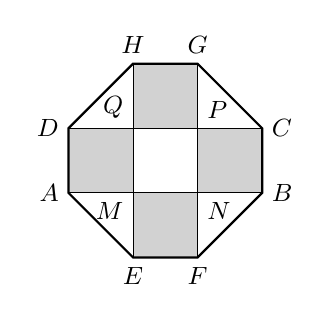
\begin{tikzpicture}[scale=0.82, every node/.style={font=\small}]
  \fill[gray!35] (-1.5,-0.5) rectangle (1.5,0.5);
  \fill[gray!35] (-0.5,-1.5) rectangle (0.5,1.5);
  % 中心正方形 MNPQ 原卷不涂阴影，照原卷留白：
  \fill[white] (-0.5,-0.5) rectangle (0.5,0.5);
  \draw[thick] (-1.5,0.5)--(-0.5,1.5)--(0.5,1.5)--(1.5,0.5)--(1.5,-0.5)--(0.5,-1.5)--(-0.5,-1.5)--(-1.5,-0.5)--cycle;
  \draw (-1.5,-0.5) rectangle (1.5,0.5);
  \draw (-0.5,-1.5) rectangle (0.5,1.5);
  \node[left] at (-1.5,0.5) {$D$};
  \node[left] at (-1.5,-0.5) {$A$};
  \node[right] at (1.5,0.5) {$C$};
  \node[right] at (1.5,-0.5) {$B$};
  \node[above] at (-0.5,1.5) {$H$};
  \node[above] at (0.5,1.5) {$G$};
  \node[below] at (-0.5,-1.5) {$E$};
  \node[below] at (0.5,-1.5) {$F$};
  \node[below left] at (-0.5,-0.5) {$M$};
  \node[below right] at (0.5,-0.5) {$N$};
  \node[above right] at (0.5,0.5) {$P$};
  \node[above left] at (-0.5,0.5) {$Q$};
\end{tikzpicture}
\end{center}

\begin{enumerate}[label=(\arabic*)]
\item 设 $DQ$ 长为 $y$（单位：m），用 $x$ 表示 $y$，并求出 $x$ 的取值范围；
\item $AD$ 取何值时可使总造价最低，并求出最低造价.
\end{enumerate}

\ifanswer
\solbegin
\stepm{(1)}{设 $AD=x\text{m}$（$x>0$），$DQ=y\text{m}$（$y>0$），}
\step{因为十字形区域总面积为 $200\text{m}^2$，所以 $4xy+x^2=200$，}
\step{解得 $y=\dfrac{200-x^2}{4x}=\dfrac{50}{x}-\dfrac{x}{4}$，}
\step{因为 $x>0$，$y>0$，所以 $y=\dfrac{200-x^2}{4x}>0$，解得 $0<x<10\sqrt2$，}
\step{所以 $y=\dfrac{50}{x}-\dfrac{x}{4}$，$0<x<10\sqrt2$；}
\stepm{(2)}{中心正方形 $MNPQ$ 区域，造价为 $2100$ 元$/\text{m}^2$，}
\step{中心正方形 $MNPQ$ 面积为 $S_1=x^2$，造价为 $W_1=2100\times S_1=2100x^2$；}
\step{周围四个矩形区域（图中阴影部分）铺设透水地砖，造价为 $105$ 元$/\text{m}^2$，}
\step{四个矩形的总面积为 $S_2=4xy=4x\left(\dfrac{50}{x}-\dfrac{x}{4}\right)=200-x^2$，}
\step{造价为 $W_2=105\times S_2=105(200-x^2)=21000-105x^2$；}
\step{四个三角形区域种植耐旱固碳植物，助力碳中和，造价为 $40$ 元$/\text{m}^2$，}
\step{四个三角形的总面积为 $S_3=4\times\dfrac12y^2=2\left(\dfrac{50}{x}-\dfrac{x}{4}\right)^2
=\dfrac{5000}{x^2}-50+\dfrac{x^2}{8}$，}
\step{造价为 $W_3=40\times S_3=40\left(\dfrac{5000}{x^2}-50+\dfrac{x^2}{8}\right)
=\dfrac{200000}{x^2}-2000+5x^2$；}
\step{设总造价为 $W$（单位：元），}
\step{则总造价为 $W=W_1+W_2+W_3$}
\step{$=2100x^2+21000-105x^2+\dfrac{200000}{x^2}-2000+5x^2$}
\step{$=2000x^2+\dfrac{200000}{x^2}+19000$，}
\step{又 $2000x^2+\dfrac{200000}{x^2}\geqslant2\sqrt{2000x^2\times\dfrac{200000}{x^2}}=2\times20000=40000$，}
\step{当且仅当 $2000x^2=\dfrac{200000}{x^2}$，即 $x=\sqrt{10}$（在 $x$ 的范围内）时取等号，}
\step{所以 $W=2000x^2+\dfrac{200000}{x^2}+19000\geqslant59000$，当 $x=\sqrt{10}$ 时取等号，}
\step{故当 $AD$ 的长为 $\sqrt{10}$ 时，总造价最低，为 $59000$ 元.}
\solend

\fi

\ansspace[8]

\item 对于实数 $a$、$b$、$c$，若 $|a-c|<|b-c|$，则称 $a$ 比 $b$ 更接近于 $c$. 现已知 $p$、$q$ 都是正有理数.

\begin{enumerate}[label=(\arabic*)]
\item 证明：$\sqrt3$ 必在 $\dfrac pq$ 和 $\dfrac{p+3q}{p+q}$ 之间；
\item 试问 $\dfrac pq$ 和 $\dfrac{p+3q}{p+q}$ 这两个数，哪一个更接近于 $\sqrt3$？说明你的理由；
\item 请你再写出一个有理数，使得它的值比 $\dfrac pq$ 和 $\dfrac{p+3q}{p+q}$ 的值更接近于 $\sqrt3$，并说明你的理由.
\end{enumerate}

\ifanswer
\solbegin
\stepm{(1)}{设 $a=\dfrac pq$（$a$ 为正有理数），则需证 $\sqrt3$ 在 $a$ 和 $\dfrac{a+3}{a+1}$（即 $\dfrac{p+3q}{p+q}$）之间.}
\step{当 $a>\sqrt3$ 时，计算 $a-\dfrac{a+3}{a+1}$ 得 $a-\dfrac{a+3}{a+1}=\dfrac{a(a+1)-(a+3)}{a+1}=\dfrac{a^2-3}{a+1}$，}
\step{$a>\sqrt3$，则 $a^2-3>0$，故 $a>\dfrac{a+3}{a+1}$；}
\step{再计算 $\dfrac{a+3}{a+1}-\sqrt3$ 得 $\dfrac{a+3}{a+1}-\sqrt3=\dfrac{(1-\sqrt3)(a-\sqrt3)}{a+1}$，}
\step{$1-\sqrt3<0$，$a-\sqrt3>0$，$a+1>0$，}
\step{故 $\dfrac{a+3}{a+1}-\sqrt3<0$，即 $\dfrac{a+3}{a+1}<\sqrt3$，从而 $\dfrac{a+3}{a+1}<\sqrt3<a$；}
\step{当 $a<\sqrt3$ 时，同理可得 $a<\dfrac{a+3}{a+1}$ 且 $\dfrac{a+3}{a+1}>\sqrt3$，即 $a<\sqrt3<\dfrac{a+3}{a+1}$，}
\step{综上，$\sqrt3$ 必在 $\dfrac pq$ 和 $\dfrac{p+3q}{p+q}$ 之间；}
\stepm{(2)}{设 $a=\dfrac pq$，$b=\dfrac{p+3q}{p+q}=\dfrac{a+3}{a+1}$，比较 $|a-\sqrt3|$ 与 $|b-\sqrt3|$，}
\step{由（1）得 $(a-\sqrt3)(b-\sqrt3)<0$，}
\step{$\dfrac{|b-\sqrt3|}{|a-\sqrt3|}
=\left|\dfrac{b-\sqrt3}{a-\sqrt3}\right|
=\dfrac{\left|\dfrac{(1-\sqrt3)(a-\sqrt3)}{a+1}\right|}{|a-\sqrt3|}
=\dfrac{\sqrt3-1}{a+1}$，}
\step{$a>0$，$a+1>1$，$\sqrt3-1<1$，故 $\dfrac{\sqrt3-1}{a+1}<1$，即 $|b-\sqrt3|<|a-\sqrt3|$，}
\step{即 $\dfrac{p+3q}{p+q}$ 比 $\dfrac pq$ 更接近于 $\sqrt3$；}
\stepm{(3)}{$\dfrac{2p+3q}{p+2q}$，理由：}
\step{设 $b=\dfrac{p+3q}{p+q}$，新数 $c=\dfrac{b+3}{b+1}=\dfrac{2p+3q}{p+2q}$，}
\step{由（1）得 $(b-\sqrt3)(c-\sqrt3)<0$，}
\step{$c-\sqrt3=\dfrac{b+3}{b+1}-\sqrt3=\dfrac{(1-\sqrt3)(b-\sqrt3)}{b+1}$，}
\step{则 $\dfrac{|c-\sqrt3|}{|b-\sqrt3|}
=\left|\dfrac{c-\sqrt3}{b-\sqrt3}\right|
=\dfrac{\left|\dfrac{(1-\sqrt3)(b-\sqrt3)}{b+1}\right|}{|b-\sqrt3|}
=\dfrac{\sqrt3-1}{b+1}$，}
\step{$b>0$，$b+1>1$，$0<\sqrt3-1<1$，故 $\dfrac{\sqrt3-1}{b+1}<1$，即 $|c-\sqrt3|<|b-\sqrt3|$，}
\step{即 $\dfrac{2p+3q}{p+2q}$ 比 $\dfrac{p+3q}{p+q}$ 更接近于 $\sqrt3$，故 $c$ 更接近 $\sqrt3$.}
\solend

\fi

\ansspace*[10]

\end{enumerate}

\end{document}
"
%
% 原始材料是微信公众号图文（公众号“魔都数学加油站”，作者“破晓”，2026-10-02 17:56 发布，
% 连载“27学年高一45”，原文标题“27学年高一45——2026-2027年上海市交附闵行高一上国庆作业2”，
% https://mp.weixin.qq.com/s/1xdCtzH-3Il0jJrz3saiPA），正文为 10 张 PNG 页。
% 第 01—06、09 页为 4762×6735；第 07、08、10 页为 2560×3620（同一篇各页原图分辨率不一致）。
% 原文本身是一份讲评版：第 3—21 题均照原卷保留题目与题下解析；第 13 题原卷把答案 C 印在括号中。
% 题目、选项、答案与解析均照原卷录入，未改内容；卷面的粉色斜水印及页脚不录入。
%
% 卷首标题：原卷印作“2026-2027 年交附闵行高一上国庆作业 2”（公众号标题里的“上海市”
% 三字卷面标题行没有，本稿照卷面），年份区间按全稿惯例排 en dash，前缀照原卷保留“年”。
%
% 与原卷的排版差异：
%   ① 原卷印有“一、填空题”“二、选择题”“三、解答题”三节标题，本稿照原卷分节，
%      只把标题改排成全稿统一的“大节标题”样式；
%   ② 第 13 题原卷在题干括号内直接印答案 C，本稿按全稿样式将括号留空、答案移入答案版的 \ans{}；
%   ③ 原卷填空横线及选择题答案括号均按全稿样式排版，填空横线统一用 \blankline[4.4em]；
%   ④ 原卷第 20 题配有十字形广场示意图，本稿在源码中用 TikZ 重绘，图中区域、边界及点名照原卷。
%   ⑤ 原卷未印副标题，本稿按本卷实际涉及的知识模块补出“集合与常用逻辑用语、不等式”。
%
% 原卷存疑/错误（均照抄原卷、未改，见对应题目处上方注释）：
%   ① 第 11 题解析原卷印"所以 p=3+9=12，又 12,15∉A，所以 12,15∉B"，与 A∪\overline{B} 的条件
%      及后文 B 的根为 6、9 均一致，无矛盾，本稿照录（早前记录的"∈B／前后矛盾"系本稿误读）；
%   ② 第 15 题题干与解析均按原卷印 ac<0，解析"因为 a<b<c，且 ac<0，所以 a<0，c>0"与题设一致，
%      无矛盾（早前记录的"abc<0／解析冲突"系本稿误读题干所致）；本稿照录原卷答案与解析。
%   ③ 第 20 题原卷各数（造价 2100 元/m^2、W_1=2100x^2、合并式 2000x^2+200000/x^2+19000、
%      末句 59000 元）经复核自洽，无矛盾（早前记录的"W_1=200x^2／末句 5900 元"系本稿误录）；本稿照录。
%   ④ 第 18(2) 题 a=-1 时 A=B=(-1,1)，不满足“B 是 A 的真子集”，故原解析给出的 a≤-1 应为 a<-1；
%   ⑤ 第 19(2) 题原卷用"{c|0<c<1}∩{c|c<-2√3/3 或 c>2√3/3}=∅"论证"不等式①、②中至多有一个恒成立"，
%      论证成立（早前记录的"区间并集留有间隙"系本稿误录解析所致）；本稿照录原卷。
%
\documentclass[a4paper,11pt]{article}
\usepackage{common}

\begin{document}

\examtitlest[3]{2026--2027 年交附闵行高一上国庆作业 2}{集合与常用逻辑用语、不等式}

\bigsec{一、填空题}

\begin{enumerate}
\setcounter{enumi}{2}

\item 满足 $A\cup\{-1,1\}=\{-1,0,1\}$ 的集合 $A$ 共有 \blankline[4.4em] 个.

\ifanswer
\solbegin
\step{集合可能为 $\{0\}$、$\{0,1\}$、$\{0,-1\}$、$\{0,1,-1\}$，共有 $4$ 个.}
\solend

\fi

\item 设 $x\in\R$，则“$x+\dfrac1x>2$”是“$x\neq1$”的 \blankline[4.4em] 条件.

\ifanswer
\solbegin
\step{$x+\dfrac1x>2\Longleftrightarrow x>0$ 且 $x\neq1$，故为充分不必要条件.}
\solend

\fi

\item 已知集合 $A=\{x\mid|x-1|<a\}$，$B=\{-4,3\}$，若 $A\cap B=\varnothing$，则 $a$ 的最大值为 \blankline[4.4em].

\ifanswer
\solbegin
\step{$A=\{x\mid -a<x-1<a\}=\{x\mid1-a<x<1+a\}$，$B=\{-4,3\}$，且 $A\cap B=\varnothing$，}
\step{$A=\varnothing$ 时，$1-a\geqslant1+a$，解得 $a\leqslant0$，满足 $A\cap B=\varnothing$；}
\step{若 $-4\in A$，则 $1-a<-4<1+a$，解得 $a>5$；}
\step{若 $3\in A$，则 $1-a<3<1+a$，解得 $a>2$，}
\step{因为 $A\cap B=\varnothing$，所以 $-4\notin A$ 且 $3\notin A$，所以 $a\leqslant5$ 且 $a\leqslant2$，所以 $a\leqslant2$，}
\step{综上，$a$ 的最大值为 $2$.}
\solend

\fi

\item 设 $x\in\R$，方程 $|x-1|+|2x-1|=|3x-2|$ 的解集为 \blankline[4.4em].

\ifanswer
\solbegin
\step{因为 $|x-1|+|2x-1|\geqslant|(x-1)+(2x-1)|=|3x-2|$，}
\step{当且仅当 $(x-1)(2x-1)\geqslant0$，解得 $x\leqslant\dfrac12$ 或 $x\geqslant1$，}
\step{故方程 $|x-1|+|2x-1|=|3x-2|$ 的解集为 $\left(-\infty,\dfrac12\right]\cup[1,+\infty)$.}
\solend

\fi

\item 已知 $a$、$b\in\R$，且 $3a+2b=1$，则 $8^a+4^b$ 最小值为 \blankline[4.4em].

\ifanswer
\solbegin
% 注：原卷本行与上行均作“$8^a+4^b$ 最小值为”，“最小值”前无“的”，原卷如此，照录未改。
\step{因为 $3a+2b=1$，所以 $8^a+4^b=2^{3a}+2^{2b}\geqslant2\sqrt{2^{3a+2b}}=2\sqrt2$，}
\step{当且仅当 $3a=2b$ 时取等号，故 $8^a+4^b$ 最小值为 $2\sqrt2$.}
\solend

\fi

\item 已知 $a>0$，$b>0$，且 $a+2b+ab=30$，则 $2a+b$ 的最小值为 \blankline[4.4em].

\ifanswer
\solbegin
\step{由 $a+2b+ab=30$，得 $(a+2)(b+1)=32$.}
\step{因为 $a>0$，$b>0$，所以 $a+2>0$，$b+1>0$，}
\step{所以 $2a+b=2(a+2)+(b+1)-5\geqslant2\sqrt{2\times32}-5=11$，}
\step{当且仅当 $2(a+2)=(b+1)$，即 $a=2$，$b=7$ 时取等号，}
\step{所以 $2a+b$ 的最小值为 $11$.}
\solend

\fi

\item 已知 $A=\{x\mid x^2+px+1=0\}$，$M=\{x\mid x>0\}$，若 $A\cap M=\varnothing$，则实数 $p$ 的取值范围为 \blankline[4.4em].

\ifanswer
\solbegin
\step{①当 $A=\varnothing$ 时，$\Delta=p^2-4<0$，所以 $-2<p<2$，此时满足 $A\cap M=\varnothing$；}
\step{②当 $A\neq\varnothing$ 时，$\Delta=p^2-4\geqslant0$，$p\geqslant2$ 或 $p\leqslant-2$，}
\step{因为 $M=\{x\mid x>0\}$，$A\cap M=\varnothing$，由韦达定理得 $\begin{cases}-p\leqslant0\\1>0\end{cases}$，解得 $p\geqslant0$，}
\step{所以 $p\geqslant2$，}
\step{由①②综合得 $p>-2$，故实数 $p$ 的取值范围为 $(-2,+\infty)$.}
\solend

\fi

\item 已知集合 $A=[t,t+1]\cup[t+3,t+6]$，其中 $t>0$. 若存在正数 $\lambda$，使得对任意 $a\in A$，都有 $\dfrac{\lambda}{a}\in A$，则 $t$ 的取值集合为 \blankline[4.4em].

\ifanswer
\solbegin
\step{因为 $0\notin A$，$t>0$，所以 $a\in[t,t+1]\cup[t+3,t+6]$，}
\step{则 $\dfrac1a\in\left[\dfrac1{t+6},\dfrac1{t+3}\right]\cup\left[\dfrac1{t+1},\dfrac1t\right]$，}
\step{又因为 $\lambda>0$，所以 $\dfrac{\lambda}{a}\in\left[\dfrac{\lambda}{t+6},\dfrac{\lambda}{t+3}\right]\cup\left[\dfrac{\lambda}{t+1},\dfrac{\lambda}{t}\right]$，}
\step{因为 $\dfrac{\lambda}{a}\in A$，所以 $\begin{cases}\dfrac{\lambda}{t+6}\geqslant t\\[3pt]\dfrac{\lambda}{t+3}\leqslant t+1\end{cases}$ 且 $\begin{cases}\dfrac{\lambda}{t+1}\geqslant t+3\\[3pt]\dfrac{\lambda}{t}\leqslant t+6\end{cases}$，}
% 注：原卷本行两个不等式组印作“$t(t+6)\leqslant\lambda\leqslant t(t+6)$”与
%     “$(t+1)(t+3)\leqslant\lambda\leqslant(t+1)(t+3)$”（两侧同式），与上行两式推导不合，系原卷笔误；
%     原卷如此，照录未改。
\step{得 $\begin{cases}t(t+6)\leqslant\lambda\leqslant t(t+6)\\[3pt](t+1)(t+3)\leqslant\lambda\leqslant(t+1)(t+3)\end{cases}$，所以 $\lambda=t(t+6)=(t+1)(t+3)$，}
\step{解得 $t=\dfrac32$，取值集合为 $\left\{\dfrac32\right\}$.}
\solend

\fi

\item 已知全集 $U=\{x\mid x=3n,1\leqslant n\leqslant5\ \text{且}\ n\in\N\}$，$A=\{x\mid x^2-px+27=0,p\in\N\}$，
$B=\{x\mid x^2-15x+q=0,q\in\N\}$，且 $A\cup\overline{B}=\{3,9,12,15\}$，则 $p+q$ 的值为 \blankline[4.4em].

\ifanswer
\solbegin
\step{因为全集 $U=\{3,6,9,12,15\}$，$A\cup\overline{B}=\{3,9,12,15\}$，}
\step{所以 $3$、$9$、$12$、$15$ 中可能有两个属于 $A$，}
\step{因为 $A$ 中的方程 $x^2-px+27=0$ 中，两根之积 $x_1x_2=27$，所以 $3$、$9\in A$，}
\step{所以 $p=3+9=12$，又 $12$、$15\notin A$，所以 $12$、$15\notin B$，}
\step{因为 $B$ 中的方程 $x^2-15x+q=0$ 中，两根之和 $x_3+x_4=15$，所以 $6$、$9\in B$，}
\step{则 $q=6\times9=54$，所以 $p+q=66$.}
\solend

\fi

\item 若关于 $x$ 的不等式 $|x-2k|+|x-3k|<4k$ 共有 $2025$ 个整数解，则实数 $k$ 的取值范围为 \blankline[4.4em].

\ifanswer
\solbegin
\step{显然 $k>0$，由 $|x-2k|+|x-3k|<4k$，得 $\dfrac{k}{2}<x<\dfrac{9k}{2}$，}
\step{因为该不等式共有 $2025$ 个整数解，所以 $2024<\dfrac{9k}{2}-\dfrac{k}{2}\leqslant2026$，}
\step{解得 $506<k\leqslant506.5$，}
\step{由 $\dfrac{k}{2}\in(253,253.25]$，得这 $2025$ 个整数解只能为 $254,255,256,\cdots,2278$，}
\step{所以 $2278<\dfrac{9k}{2}\leqslant2279$，解得 $506\dfrac29<k\leqslant506\dfrac49$，结合 $506<k\leqslant506.5$，}
\step{得 $k$ 的取值范围是 $\left(506\dfrac29,506\dfrac49\right]$.}
\solend

\fi

\end{enumerate}

\bigsec{二、选择题}

\begin{enumerate}
\setcounter{enumi}{12}

\item 已知 $a,b\in\R$，且 $ab\neq0$，则下列结论恒成立的是\mbox{（\quad）}

\keepwithprev
A. $a+b\geqslant2\sqrt{ab}$\qquad
B. $\left(\dfrac{a+b}{2}\right)^2>ab$\qquad
C. $\left|\dfrac ab+\dfrac ba\right|\geqslant2$\qquad
D. $a^2+b^2>2ab$

\ans{$C$}

\item 如果 $a^{2025}+b^{2025}=0$，那么一定有\mbox{（\quad）}

\keepwithprev
A. $(|a|+|b|)^{2025}=0$\qquad
B. $(a-b)^{2025}=0$\qquad
C. $(a\cdot b)^{2025}=0$\qquad
D. $(a+b)^{2025}=0$

\ans{$D$}

\ifanswer
\solbegin
\step{由 $a^{2025}+b^{2025}=0$，得 $a^{2025}=-b^{2025}=(-b)^{2025}$，则 $\left(a^{2025}\right)^{\frac{1}{2025}}=\left[(-b)^{2025}\right]^{\frac{1}{2025}}$，}
\step{即 $a=-b$，即 $a+b=0$，故 $(a+b)^{2025}=0$，故 D 符合题意；}
\step{对于 A，若取 $a=1$，$b=-1$，则 $(|a|+|b|)^{2025}=2^{2025}\neq0$，故 A 不合题意；}
\step{对于 B，若取 $a=1$，$b=-1$，则 $(a-b)^{2025}=2^{2025}\neq0$，故 B 不合题意；}
\step{对于 C，若取 $a=1$，$b=-1$，则 $(a\cdot b)^{2025}=(-1)^{2025}=-1\neq0$，故 C 不合题意；}
\step{故选 D.}
\solend

\fi

\item 已知 $a$、$b$、$c$ 满足 $a<b<c$，且 $ac<0$，那么下列各式中一定成立的是\mbox{（\quad）}

\keepwithprev
A. $\dfrac1a>\dfrac1c$\qquad
B. $ab^2<cb^2$\qquad
C. $ac<bc$\qquad
D. $a+c>2b$

\ans{$C$}

\ifanswer
\solbegin
\step{因为 $a<b<c$，且 $ac<0$，所以 $a<0$，$c>0$，}
\step{对于 A，$\dfrac1a<0<\dfrac1c$，故 A 错误；}
\step{对于 B，当 $b=0$ 时，$ab^2=cb^2$，故 B 错误；}
\step{对于 C，$ac<bc$ 可化为 $(a-b)c<0$，因为 $a<b$，所以 $a-b<0$，}
\step{又因为 $c>0$，所以 $(a-b)c<0$，所以 C 正确；}
\step{对于 D，设 $a=-2$，$b=0$，$c=1$，则 $a+c<2b$，故 D 错误.}
\step{故选 C.}
\solend

\fi

\item 对于 $a\in\R$，设集合 $A=\left\{x\mid\dfrac{(x^2-6x+a)(x-1)}{x+a}=0\right\}$，记 $A$ 的所有元素之和为 $S(a)$，
所有元素之积为 $T(a)$，则下列说法中，正确的是\mbox{（\quad）}

\keepwithprev
A. 不存在实数 $a$，使得 $S(a)=6$\qquad
B. 存在实数 $a$，使得 $T(a)=9$

C. 存在无数实数 $a$，使得 $S(a)=7$\qquad
D. 若 $T(a)=3$，则 $a=3$

\ans{$C$}

\ifanswer
\solbegin
\step{要使 $\dfrac{(x^2-6x+a)(x-1)}{x+a}=0$，只需 $(x^2-6x+a)(x-1)=0$ 且 $x+a\neq0$，}
\step{由 $(x^2-6x+a)(x-1)=0$ 得 $x^2-6x+a=0$ 或 $x-1=0$，}
\step{对于一元二次方程 $x^2-6x+a=0$，其判别式 $\Delta=36-4a$，}
\step{当 $\Delta=0$，即 $a=9$ 时，集合 $A=\{1,3\}$，$S(a)=4$，$T(a)=3$；}
\step{当 $\Delta<0$，即 $a>9$ 时，集合 $A=\{1\}$，$S(a)=T(a)=1$；}
\step{当 $\Delta>0$，即 $a<9$ 时，一元二次方程 $x^2-6x+a=0$ 的解为 $x=3\pm\sqrt{9-a}$，}
\step{①当 $a=0$ 时，$x\neq0$，则集合 $A=\{1,6\}$，则 $S(a)=7$，$T(a)=6$，}
\step{②当 $a=-7$ 时，$x\neq7$，则集合 $A=\{-1,1\}$，则 $S(a)=0$，$T(a)=-1$，}
% 注：下一行集合 A 原卷印作 {-1,1}（按 a=-1 代入 x^2-6x-1=0 应得 3±√10，原卷如此，照录未改）。
\step{③当 $a=-1$ 时，$x\neq1$，则集合 $A=\{-1,1\}$，则 $S(a)=6$，$T(a)=-1$，}
\step{④当 $a=5$ 时，$x\neq-5$，则集合 $A=\{1,5\}$，则 $S(a)=6$，$T(a)=5$，}
\step{⑤当 $a\neq5,0,-1,-7$ 时，集合 $A=\{1,3-\sqrt{9-a},3+\sqrt{9-a}\}$，}
\step{则 $S(a)=7$，$T(a)=a$.}
\step{选项 A，当 $a=5$ 时，$S(a)=6$，所以 A 错误；}
\step{选项 B，$T(a)$ 的可能值为 $-1,1,3,5,6,a$（$a<9$），无 $T(a)=9$，所以 B 错误；}
\step{选项 C，当 $a<9$，且 $a\neq5,-1,-7$ 时，$S(a)=7$，有无数个 $a$ 满足，所以 C 正确；}
\step{选项 D，当 $T(a)=3$ 时，有 $a=3$ 和 $a=9$ 满足，所以 D 错误.}
\step{故选 C.}
\solend

\fi

\end{enumerate}

\bigsec{三、解答题}

\begin{enumerate}
\setcounter{enumi}{16}

\item 已知 $a\in\R$，关于 $x$ 的不等式 $|x+1|+|x-1|>a^2-5a+4$.

\begin{enumerate}[label=(\arabic*)]
\item 当 $a=0$ 时，求不等式的解集；
\item 若不等式的解集为 $\R$，求 $a$ 的取值范围.
\end{enumerate}

\ifanswer
\solbegin
\stepm{(1)}{当 $a=0$ 时，不等式为 $|x+1|+|x-1|>4$，}
\step{又 $|x+1|+|x-1|=\begin{cases}2x,&x\geqslant1\\2,&-1<x<1\\-2x,&x\leqslant-1\end{cases}$，}
\step{则 $|x+1|+|x-1|>4$ 的解为 $x>2$ 或 $x<-2$，}
\step{即不等式的解集为 $(-\infty,-2)\cup(2,+\infty)$；}
\stepm{(2)}{不等式 $|x+1|+|x-1|>a^2-5a+4$ 的解集为 $\R$，}
\step{则 $(|x+1|+|x-1|)_{\min}>a^2-5a+4$，}
\step{又 $(|x+1|+|x-1|)_{\min}=2$，当且仅当 $-1\leqslant x\leqslant1$ 时取得，即 $a^2-5a+4<2$，}
\step{即 $a^2-5a+2<0$，即 $\dfrac{5-\sqrt{17}}2<a<\dfrac{5+\sqrt{17}}2$，}
\step{即 $a$ 的取值范围为 $\left(\dfrac{5-\sqrt{17}}2,\dfrac{5+\sqrt{17}}2\right)$.}
\solend

\fi

\ansspace[6]

\item 已知集合 $A=\{x\mid(x-a)(x-a^2)<0\}$，集合 $B=\left\{x\mid\dfrac{2x}{x-1}<1\right\}$，命题 $p:x\in A$，命题 $q:x\in B$.

\begin{enumerate}[label=(\arabic*)]
\item 当实数 $a$ 为何值时，$A=B$；
\item 若 $q$ 是 $p$ 的充分不必要条件，求实数 $a$ 的取值范围.
\end{enumerate}

\ifanswer
\solbegin
\stepm{(1)}{由 $\dfrac{2x}{x-1}<1$ 得 $\dfrac{2x}{x-1}-1=\dfrac{x+1}{x-1}<0$，解得 $-1<x<1$，即 $B=\{x\mid-1<x<1\}$，}
\step{因为 $A=\{x\mid(x-a)(x-a^2)<0\}$，$A=B$，所以 $\begin{cases}a=-1\\a^2=1\end{cases}$，解得 $a=-1$；}
\stepm{(2)}{若 $q$ 是 $p$ 的充分不必要条件，则 $B\subset A$，}
\step{当 $a^2=a$，即 $a=0$ 或 $a=1$ 时，$A=\varnothing$，显然不符合题意；}
\step{当 $a^2>a$，即 $a>1$ 或 $a<0$ 时，$A=(a,a^2)$，则 $\begin{cases}a\leqslant-1\\a^2\geqslant1\\a>1\ \text{或}\ a<0\end{cases}$，}
% 注：a=-1 时 A=(-1,1)=B，不是 B 的真子集；原解析用 B⊂A 但答案含 -1，照录。
\step{前两等号不能同时取得，解得 $a\leqslant-1$；}
\step{当 $a^2<a$，即 $0<a<1$ 时，$A=(a^2,a)$，显然不符合题意，}
\step{故 $a$ 的范围为 $\{a\mid a\leqslant-1\}$.}
\solend

\fi

\ansspace[6]

\item 已知不等式① $x^2+2cx+c>0$，② $x^2+cx+c^2-1>0$，其中 $c$ 是实数.

\begin{enumerate}[label=(\arabic*)]
\item 若 $1$ 是不等式②的一个解，求实数 $c$ 的取值范围；
\item 证明：不等式①、②中至多有一个恒成立.
\end{enumerate}

\ifanswer
\solbegin
\stepm{(1)}{已知不等式① $x^2+2cx+c>0$，② $x^2+cx+c^2-1>0$，}
\step{又 $1$ 是不等式②的一个解，则 $1+c+c^2-1>0$，}
\step{则 $c^2+c>0$，则 $c<-1$ 或 $c>0$，则 $c$ 的取值范围为 $(-\infty,-1)\cup(0,+\infty)$；}
\stepm{(2)}{若不等式①恒成立，则 $\Delta=4c^2-4c<0$，则 $0<c<1$，}
\step{若不等式②恒成立，则 $\Delta=c^2-4(c^2-1)=4-3c^2<0$，}
\step{则 $c<-\dfrac{2\sqrt3}{3}$ 或 $c>\dfrac{2\sqrt3}{3}$，}
\step{又 $\{c\mid 0<c<1\}\cap\left\{c\mid c<-\dfrac{2\sqrt3}{3}\ \text{或}\ c>\dfrac{2\sqrt3}{3}\right\}=\varnothing$，}
\step{则不存在实数 $c$ 使得不等式①、②同时恒成立，}
\step{则不等式①、②中至多有一个恒成立.}
\solend

\fi

\ansspace[6]

\item 为践行“科技强国”战略，某社区计划建造一座融合智慧节能技术的八边形休闲广场，其中两个相同的矩形 $ABCD$ 和 $EFGH$ 构成的十字形区域总面积为 $200\text{m}^2$. 中心正方形 $MNPQ$ 区域将安装国产太阳能光伏板（兼具休憩遮阳功能），造价为 $2100$ 元$/\text{m}^2$；周围四个矩形区域（图中阴影部分）铺设透水地砖，造价为 $105$ 元$/\text{m}^2$；再在四个三角形区域种植耐旱固碳植物，助力碳中和，造价为 $40$ 元$/\text{m}^2$. 设总造价为 $W$（单位：元），$AD=x$（单位：m）.

\begin{center}
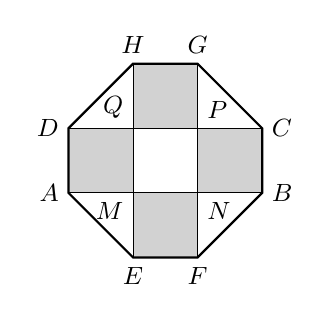
\begin{tikzpicture}[scale=0.82, every node/.style={font=\small}]
  \fill[gray!35] (-1.5,-0.5) rectangle (1.5,0.5);
  \fill[gray!35] (-0.5,-1.5) rectangle (0.5,1.5);
  % 中心正方形 MNPQ 原卷不涂阴影，照原卷留白：
  \fill[white] (-0.5,-0.5) rectangle (0.5,0.5);
  \draw[thick] (-1.5,0.5)--(-0.5,1.5)--(0.5,1.5)--(1.5,0.5)--(1.5,-0.5)--(0.5,-1.5)--(-0.5,-1.5)--(-1.5,-0.5)--cycle;
  \draw (-1.5,-0.5) rectangle (1.5,0.5);
  \draw (-0.5,-1.5) rectangle (0.5,1.5);
  \node[left] at (-1.5,0.5) {$D$};
  \node[left] at (-1.5,-0.5) {$A$};
  \node[right] at (1.5,0.5) {$C$};
  \node[right] at (1.5,-0.5) {$B$};
  \node[above] at (-0.5,1.5) {$H$};
  \node[above] at (0.5,1.5) {$G$};
  \node[below] at (-0.5,-1.5) {$E$};
  \node[below] at (0.5,-1.5) {$F$};
  \node[below left] at (-0.5,-0.5) {$M$};
  \node[below right] at (0.5,-0.5) {$N$};
  \node[above right] at (0.5,0.5) {$P$};
  \node[above left] at (-0.5,0.5) {$Q$};
\end{tikzpicture}
\end{center}

\begin{enumerate}[label=(\arabic*)]
\item 设 $DQ$ 长为 $y$（单位：m），用 $x$ 表示 $y$，并求出 $x$ 的取值范围；
\item $AD$ 取何值时可使总造价最低，并求出最低造价.
\end{enumerate}

\ifanswer
\solbegin
\stepm{(1)}{设 $AD=x\text{m}$（$x>0$），$DQ=y\text{m}$（$y>0$），}
\step{因为十字形区域总面积为 $200\text{m}^2$，所以 $4xy+x^2=200$，}
\step{解得 $y=\dfrac{200-x^2}{4x}=\dfrac{50}{x}-\dfrac{x}{4}$，}
\step{因为 $x>0$，$y>0$，所以 $y=\dfrac{200-x^2}{4x}>0$，解得 $0<x<10\sqrt2$，}
\step{所以 $y=\dfrac{50}{x}-\dfrac{x}{4}$，$0<x<10\sqrt2$；}
\stepm{(2)}{中心正方形 $MNPQ$ 区域，造价为 $2100$ 元$/\text{m}^2$，}
\step{中心正方形 $MNPQ$ 面积为 $S_1=x^2$，造价为 $W_1=2100\times S_1=2100x^2$；}
\step{周围四个矩形区域（图中阴影部分）铺设透水地砖，造价为 $105$ 元$/\text{m}^2$，}
\step{四个矩形的总面积为 $S_2=4xy=4x\left(\dfrac{50}{x}-\dfrac{x}{4}\right)=200-x^2$，}
\step{造价为 $W_2=105\times S_2=105(200-x^2)=21000-105x^2$；}
\step{四个三角形区域种植耐旱固碳植物，助力碳中和，造价为 $40$ 元$/\text{m}^2$，}
\step{四个三角形的总面积为 $S_3=4\times\dfrac12y^2=2\left(\dfrac{50}{x}-\dfrac{x}{4}\right)^2
=\dfrac{5000}{x^2}-50+\dfrac{x^2}{8}$，}
\step{造价为 $W_3=40\times S_3=40\left(\dfrac{5000}{x^2}-50+\dfrac{x^2}{8}\right)
=\dfrac{200000}{x^2}-2000+5x^2$；}
\step{设总造价为 $W$（单位：元），}
\step{则总造价为 $W=W_1+W_2+W_3$}
\step{$=2100x^2+21000-105x^2+\dfrac{200000}{x^2}-2000+5x^2$}
\step{$=2000x^2+\dfrac{200000}{x^2}+19000$，}
\step{又 $2000x^2+\dfrac{200000}{x^2}\geqslant2\sqrt{2000x^2\times\dfrac{200000}{x^2}}=2\times20000=40000$，}
\step{当且仅当 $2000x^2=\dfrac{200000}{x^2}$，即 $x=\sqrt{10}$（在 $x$ 的范围内）时取等号，}
\step{所以 $W=2000x^2+\dfrac{200000}{x^2}+19000\geqslant59000$，当 $x=\sqrt{10}$ 时取等号，}
\step{故当 $AD$ 的长为 $\sqrt{10}$ 时，总造价最低，为 $59000$ 元.}
\solend

\fi

\ansspace[8]

\item 对于实数 $a$、$b$、$c$，若 $|a-c|<|b-c|$，则称 $a$ 比 $b$ 更接近于 $c$. 现已知 $p$、$q$ 都是正有理数.

\begin{enumerate}[label=(\arabic*)]
\item 证明：$\sqrt3$ 必在 $\dfrac pq$ 和 $\dfrac{p+3q}{p+q}$ 之间；
\item 试问 $\dfrac pq$ 和 $\dfrac{p+3q}{p+q}$ 这两个数，哪一个更接近于 $\sqrt3$？说明你的理由；
\item 请你再写出一个有理数，使得它的值比 $\dfrac pq$ 和 $\dfrac{p+3q}{p+q}$ 的值更接近于 $\sqrt3$，并说明你的理由.
\end{enumerate}

\ifanswer
\solbegin
\stepm{(1)}{设 $a=\dfrac pq$（$a$ 为正有理数），则需证 $\sqrt3$ 在 $a$ 和 $\dfrac{a+3}{a+1}$（即 $\dfrac{p+3q}{p+q}$）之间.}
\step{当 $a>\sqrt3$ 时，计算 $a-\dfrac{a+3}{a+1}$ 得 $a-\dfrac{a+3}{a+1}=\dfrac{a(a+1)-(a+3)}{a+1}=\dfrac{a^2-3}{a+1}$，}
\step{$a>\sqrt3$，则 $a^2-3>0$，故 $a>\dfrac{a+3}{a+1}$；}
\step{再计算 $\dfrac{a+3}{a+1}-\sqrt3$ 得 $\dfrac{a+3}{a+1}-\sqrt3=\dfrac{(1-\sqrt3)(a-\sqrt3)}{a+1}$，}
\step{$1-\sqrt3<0$，$a-\sqrt3>0$，$a+1>0$，}
\step{故 $\dfrac{a+3}{a+1}-\sqrt3<0$，即 $\dfrac{a+3}{a+1}<\sqrt3$，从而 $\dfrac{a+3}{a+1}<\sqrt3<a$；}
\step{当 $a<\sqrt3$ 时，同理可得 $a<\dfrac{a+3}{a+1}$ 且 $\dfrac{a+3}{a+1}>\sqrt3$，即 $a<\sqrt3<\dfrac{a+3}{a+1}$，}
\step{综上，$\sqrt3$ 必在 $\dfrac pq$ 和 $\dfrac{p+3q}{p+q}$ 之间；}
\stepm{(2)}{设 $a=\dfrac pq$，$b=\dfrac{p+3q}{p+q}=\dfrac{a+3}{a+1}$，比较 $|a-\sqrt3|$ 与 $|b-\sqrt3|$，}
\step{由（1）得 $(a-\sqrt3)(b-\sqrt3)<0$，}
\step{$\dfrac{|b-\sqrt3|}{|a-\sqrt3|}
=\left|\dfrac{b-\sqrt3}{a-\sqrt3}\right|
=\dfrac{\left|\dfrac{(1-\sqrt3)(a-\sqrt3)}{a+1}\right|}{|a-\sqrt3|}
=\dfrac{\sqrt3-1}{a+1}$，}
\step{$a>0$，$a+1>1$，$\sqrt3-1<1$，故 $\dfrac{\sqrt3-1}{a+1}<1$，即 $|b-\sqrt3|<|a-\sqrt3|$，}
\step{即 $\dfrac{p+3q}{p+q}$ 比 $\dfrac pq$ 更接近于 $\sqrt3$；}
\stepm{(3)}{$\dfrac{2p+3q}{p+2q}$，理由：}
\step{设 $b=\dfrac{p+3q}{p+q}$，新数 $c=\dfrac{b+3}{b+1}=\dfrac{2p+3q}{p+2q}$，}
\step{由（1）得 $(b-\sqrt3)(c-\sqrt3)<0$，}
\step{$c-\sqrt3=\dfrac{b+3}{b+1}-\sqrt3=\dfrac{(1-\sqrt3)(b-\sqrt3)}{b+1}$，}
\step{则 $\dfrac{|c-\sqrt3|}{|b-\sqrt3|}
=\left|\dfrac{c-\sqrt3}{b-\sqrt3}\right|
=\dfrac{\left|\dfrac{(1-\sqrt3)(b-\sqrt3)}{b+1}\right|}{|b-\sqrt3|}
=\dfrac{\sqrt3-1}{b+1}$，}
\step{$b>0$，$b+1>1$，$0<\sqrt3-1<1$，故 $\dfrac{\sqrt3-1}{b+1}<1$，即 $|c-\sqrt3|<|b-\sqrt3|$，}
\step{即 $\dfrac{2p+3q}{p+2q}$ 比 $\dfrac{p+3q}{p+q}$ 更接近于 $\sqrt3$，故 $c$ 更接近 $\sqrt3$.}
\solend

\fi

\ansspace*[10]

\end{enumerate}

\end{document}
"
% 紧凑版：xelatex "\def\iscompact{1}% 高一45_交附闵行_国庆作业2.tex
%   —— 高一上数学“2026-2027 年交附闵行高一上国庆作业 2”（试卷版/答案版）
% 试卷版：xelatex 高一45_交附闵行_国庆作业2.tex
% 答案版：xelatex "\def\isanswer{1}% 高一45_交附闵行_国庆作业2.tex
%   —— 高一上数学“2026-2027 年交附闵行高一上国庆作业 2”（试卷版/答案版）
% 试卷版：xelatex 高一45_交附闵行_国庆作业2.tex
% 答案版：xelatex "\def\isanswer{1}% 高一45_交附闵行_国庆作业2.tex
%   —— 高一上数学“2026-2027 年交附闵行高一上国庆作业 2”（试卷版/答案版）
% 试卷版：xelatex 高一45_交附闵行_国庆作业2.tex
% 答案版：xelatex "\def\isanswer{1}\input{高一45_交附闵行_国庆作业2.tex}"
% 紧凑版：xelatex "\def\iscompact{1}\input{高一45_交附闵行_国庆作业2.tex}"
%
% 原始材料是微信公众号图文（公众号“魔都数学加油站”，作者“破晓”，2026-10-02 17:56 发布，
% 连载“27学年高一45”，原文标题“27学年高一45——2026-2027年上海市交附闵行高一上国庆作业2”，
% https://mp.weixin.qq.com/s/1xdCtzH-3Il0jJrz3saiPA），正文为 10 张 PNG 页。
% 第 01—06、09 页为 4762×6735；第 07、08、10 页为 2560×3620（同一篇各页原图分辨率不一致）。
% 原文本身是一份讲评版：第 3—21 题均照原卷保留题目与题下解析；第 13 题原卷把答案 C 印在括号中。
% 题目、选项、答案与解析均照原卷录入，未改内容；卷面的粉色斜水印及页脚不录入。
%
% 卷首标题：原卷印作“2026-2027 年交附闵行高一上国庆作业 2”（公众号标题里的“上海市”
% 三字卷面标题行没有，本稿照卷面），年份区间按全稿惯例排 en dash，前缀照原卷保留“年”。
%
% 与原卷的排版差异：
%   ① 原卷印有“一、填空题”“二、选择题”“三、解答题”三节标题，本稿照原卷分节，
%      只把标题改排成全稿统一的“大节标题”样式；
%   ② 第 13 题原卷在题干括号内直接印答案 C，本稿按全稿样式将括号留空、答案移入答案版的 \ans{}；
%   ③ 原卷填空横线及选择题答案括号均按全稿样式排版，填空横线统一用 \blankline[4.4em]；
%   ④ 原卷第 20 题配有十字形广场示意图，本稿在源码中用 TikZ 重绘，图中区域、边界及点名照原卷。
%   ⑤ 原卷未印副标题，本稿按本卷实际涉及的知识模块补出“集合与常用逻辑用语、不等式”。
%
% 原卷存疑/错误（均照抄原卷、未改，见对应题目处上方注释）：
%   ① 第 11 题解析原卷印"所以 p=3+9=12，又 12,15∉A，所以 12,15∉B"，与 A∪\overline{B} 的条件
%      及后文 B 的根为 6、9 均一致，无矛盾，本稿照录（早前记录的"∈B／前后矛盾"系本稿误读）；
%   ② 第 15 题题干与解析均按原卷印 ac<0，解析"因为 a<b<c，且 ac<0，所以 a<0，c>0"与题设一致，
%      无矛盾（早前记录的"abc<0／解析冲突"系本稿误读题干所致）；本稿照录原卷答案与解析。
%   ③ 第 20 题原卷各数（造价 2100 元/m^2、W_1=2100x^2、合并式 2000x^2+200000/x^2+19000、
%      末句 59000 元）经复核自洽，无矛盾（早前记录的"W_1=200x^2／末句 5900 元"系本稿误录）；本稿照录。
%   ④ 第 18(2) 题 a=-1 时 A=B=(-1,1)，不满足“B 是 A 的真子集”，故原解析给出的 a≤-1 应为 a<-1；
%   ⑤ 第 19(2) 题原卷用"{c|0<c<1}∩{c|c<-2√3/3 或 c>2√3/3}=∅"论证"不等式①、②中至多有一个恒成立"，
%      论证成立（早前记录的"区间并集留有间隙"系本稿误录解析所致）；本稿照录原卷。
%
\documentclass[a4paper,11pt]{article}
\usepackage{common}

\begin{document}

\examtitlest[3]{2026--2027 年交附闵行高一上国庆作业 2}{集合与常用逻辑用语、不等式}

\bigsec{一、填空题}

\begin{enumerate}
\setcounter{enumi}{2}

\item 满足 $A\cup\{-1,1\}=\{-1,0,1\}$ 的集合 $A$ 共有 \blankline[4.4em] 个.

\ifanswer
\solbegin
\step{集合可能为 $\{0\}$、$\{0,1\}$、$\{0,-1\}$、$\{0,1,-1\}$，共有 $4$ 个.}
\solend

\fi

\item 设 $x\in\R$，则“$x+\dfrac1x>2$”是“$x\neq1$”的 \blankline[4.4em] 条件.

\ifanswer
\solbegin
\step{$x+\dfrac1x>2\Longleftrightarrow x>0$ 且 $x\neq1$，故为充分不必要条件.}
\solend

\fi

\item 已知集合 $A=\{x\mid|x-1|<a\}$，$B=\{-4,3\}$，若 $A\cap B=\varnothing$，则 $a$ 的最大值为 \blankline[4.4em].

\ifanswer
\solbegin
\step{$A=\{x\mid -a<x-1<a\}=\{x\mid1-a<x<1+a\}$，$B=\{-4,3\}$，且 $A\cap B=\varnothing$，}
\step{$A=\varnothing$ 时，$1-a\geqslant1+a$，解得 $a\leqslant0$，满足 $A\cap B=\varnothing$；}
\step{若 $-4\in A$，则 $1-a<-4<1+a$，解得 $a>5$；}
\step{若 $3\in A$，则 $1-a<3<1+a$，解得 $a>2$，}
\step{因为 $A\cap B=\varnothing$，所以 $-4\notin A$ 且 $3\notin A$，所以 $a\leqslant5$ 且 $a\leqslant2$，所以 $a\leqslant2$，}
\step{综上，$a$ 的最大值为 $2$.}
\solend

\fi

\item 设 $x\in\R$，方程 $|x-1|+|2x-1|=|3x-2|$ 的解集为 \blankline[4.4em].

\ifanswer
\solbegin
\step{因为 $|x-1|+|2x-1|\geqslant|(x-1)+(2x-1)|=|3x-2|$，}
\step{当且仅当 $(x-1)(2x-1)\geqslant0$，解得 $x\leqslant\dfrac12$ 或 $x\geqslant1$，}
\step{故方程 $|x-1|+|2x-1|=|3x-2|$ 的解集为 $\left(-\infty,\dfrac12\right]\cup[1,+\infty)$.}
\solend

\fi

\item 已知 $a$、$b\in\R$，且 $3a+2b=1$，则 $8^a+4^b$ 最小值为 \blankline[4.4em].

\ifanswer
\solbegin
% 注：原卷本行与上行均作“$8^a+4^b$ 最小值为”，“最小值”前无“的”，原卷如此，照录未改。
\step{因为 $3a+2b=1$，所以 $8^a+4^b=2^{3a}+2^{2b}\geqslant2\sqrt{2^{3a+2b}}=2\sqrt2$，}
\step{当且仅当 $3a=2b$ 时取等号，故 $8^a+4^b$ 最小值为 $2\sqrt2$.}
\solend

\fi

\item 已知 $a>0$，$b>0$，且 $a+2b+ab=30$，则 $2a+b$ 的最小值为 \blankline[4.4em].

\ifanswer
\solbegin
\step{由 $a+2b+ab=30$，得 $(a+2)(b+1)=32$.}
\step{因为 $a>0$，$b>0$，所以 $a+2>0$，$b+1>0$，}
\step{所以 $2a+b=2(a+2)+(b+1)-5\geqslant2\sqrt{2\times32}-5=11$，}
\step{当且仅当 $2(a+2)=(b+1)$，即 $a=2$，$b=7$ 时取等号，}
\step{所以 $2a+b$ 的最小值为 $11$.}
\solend

\fi

\item 已知 $A=\{x\mid x^2+px+1=0\}$，$M=\{x\mid x>0\}$，若 $A\cap M=\varnothing$，则实数 $p$ 的取值范围为 \blankline[4.4em].

\ifanswer
\solbegin
\step{①当 $A=\varnothing$ 时，$\Delta=p^2-4<0$，所以 $-2<p<2$，此时满足 $A\cap M=\varnothing$；}
\step{②当 $A\neq\varnothing$ 时，$\Delta=p^2-4\geqslant0$，$p\geqslant2$ 或 $p\leqslant-2$，}
\step{因为 $M=\{x\mid x>0\}$，$A\cap M=\varnothing$，由韦达定理得 $\begin{cases}-p\leqslant0\\1>0\end{cases}$，解得 $p\geqslant0$，}
\step{所以 $p\geqslant2$，}
\step{由①②综合得 $p>-2$，故实数 $p$ 的取值范围为 $(-2,+\infty)$.}
\solend

\fi

\item 已知集合 $A=[t,t+1]\cup[t+3,t+6]$，其中 $t>0$. 若存在正数 $\lambda$，使得对任意 $a\in A$，都有 $\dfrac{\lambda}{a}\in A$，则 $t$ 的取值集合为 \blankline[4.4em].

\ifanswer
\solbegin
\step{因为 $0\notin A$，$t>0$，所以 $a\in[t,t+1]\cup[t+3,t+6]$，}
\step{则 $\dfrac1a\in\left[\dfrac1{t+6},\dfrac1{t+3}\right]\cup\left[\dfrac1{t+1},\dfrac1t\right]$，}
\step{又因为 $\lambda>0$，所以 $\dfrac{\lambda}{a}\in\left[\dfrac{\lambda}{t+6},\dfrac{\lambda}{t+3}\right]\cup\left[\dfrac{\lambda}{t+1},\dfrac{\lambda}{t}\right]$，}
\step{因为 $\dfrac{\lambda}{a}\in A$，所以 $\begin{cases}\dfrac{\lambda}{t+6}\geqslant t\\[3pt]\dfrac{\lambda}{t+3}\leqslant t+1\end{cases}$ 且 $\begin{cases}\dfrac{\lambda}{t+1}\geqslant t+3\\[3pt]\dfrac{\lambda}{t}\leqslant t+6\end{cases}$，}
% 注：原卷本行两个不等式组印作“$t(t+6)\leqslant\lambda\leqslant t(t+6)$”与
%     “$(t+1)(t+3)\leqslant\lambda\leqslant(t+1)(t+3)$”（两侧同式），与上行两式推导不合，系原卷笔误；
%     原卷如此，照录未改。
\step{得 $\begin{cases}t(t+6)\leqslant\lambda\leqslant t(t+6)\\[3pt](t+1)(t+3)\leqslant\lambda\leqslant(t+1)(t+3)\end{cases}$，所以 $\lambda=t(t+6)=(t+1)(t+3)$，}
\step{解得 $t=\dfrac32$，取值集合为 $\left\{\dfrac32\right\}$.}
\solend

\fi

\item 已知全集 $U=\{x\mid x=3n,1\leqslant n\leqslant5\ \text{且}\ n\in\N\}$，$A=\{x\mid x^2-px+27=0,p\in\N\}$，
$B=\{x\mid x^2-15x+q=0,q\in\N\}$，且 $A\cup\overline{B}=\{3,9,12,15\}$，则 $p+q$ 的值为 \blankline[4.4em].

\ifanswer
\solbegin
\step{因为全集 $U=\{3,6,9,12,15\}$，$A\cup\overline{B}=\{3,9,12,15\}$，}
\step{所以 $3$、$9$、$12$、$15$ 中可能有两个属于 $A$，}
\step{因为 $A$ 中的方程 $x^2-px+27=0$ 中，两根之积 $x_1x_2=27$，所以 $3$、$9\in A$，}
\step{所以 $p=3+9=12$，又 $12$、$15\notin A$，所以 $12$、$15\notin B$，}
\step{因为 $B$ 中的方程 $x^2-15x+q=0$ 中，两根之和 $x_3+x_4=15$，所以 $6$、$9\in B$，}
\step{则 $q=6\times9=54$，所以 $p+q=66$.}
\solend

\fi

\item 若关于 $x$ 的不等式 $|x-2k|+|x-3k|<4k$ 共有 $2025$ 个整数解，则实数 $k$ 的取值范围为 \blankline[4.4em].

\ifanswer
\solbegin
\step{显然 $k>0$，由 $|x-2k|+|x-3k|<4k$，得 $\dfrac{k}{2}<x<\dfrac{9k}{2}$，}
\step{因为该不等式共有 $2025$ 个整数解，所以 $2024<\dfrac{9k}{2}-\dfrac{k}{2}\leqslant2026$，}
\step{解得 $506<k\leqslant506.5$，}
\step{由 $\dfrac{k}{2}\in(253,253.25]$，得这 $2025$ 个整数解只能为 $254,255,256,\cdots,2278$，}
\step{所以 $2278<\dfrac{9k}{2}\leqslant2279$，解得 $506\dfrac29<k\leqslant506\dfrac49$，结合 $506<k\leqslant506.5$，}
\step{得 $k$ 的取值范围是 $\left(506\dfrac29,506\dfrac49\right]$.}
\solend

\fi

\end{enumerate}

\bigsec{二、选择题}

\begin{enumerate}
\setcounter{enumi}{12}

\item 已知 $a,b\in\R$，且 $ab\neq0$，则下列结论恒成立的是\mbox{（\quad）}

\keepwithprev
A. $a+b\geqslant2\sqrt{ab}$\qquad
B. $\left(\dfrac{a+b}{2}\right)^2>ab$\qquad
C. $\left|\dfrac ab+\dfrac ba\right|\geqslant2$\qquad
D. $a^2+b^2>2ab$

\ans{$C$}

\item 如果 $a^{2025}+b^{2025}=0$，那么一定有\mbox{（\quad）}

\keepwithprev
A. $(|a|+|b|)^{2025}=0$\qquad
B. $(a-b)^{2025}=0$\qquad
C. $(a\cdot b)^{2025}=0$\qquad
D. $(a+b)^{2025}=0$

\ans{$D$}

\ifanswer
\solbegin
\step{由 $a^{2025}+b^{2025}=0$，得 $a^{2025}=-b^{2025}=(-b)^{2025}$，则 $\left(a^{2025}\right)^{\frac{1}{2025}}=\left[(-b)^{2025}\right]^{\frac{1}{2025}}$，}
\step{即 $a=-b$，即 $a+b=0$，故 $(a+b)^{2025}=0$，故 D 符合题意；}
\step{对于 A，若取 $a=1$，$b=-1$，则 $(|a|+|b|)^{2025}=2^{2025}\neq0$，故 A 不合题意；}
\step{对于 B，若取 $a=1$，$b=-1$，则 $(a-b)^{2025}=2^{2025}\neq0$，故 B 不合题意；}
\step{对于 C，若取 $a=1$，$b=-1$，则 $(a\cdot b)^{2025}=(-1)^{2025}=-1\neq0$，故 C 不合题意；}
\step{故选 D.}
\solend

\fi

\item 已知 $a$、$b$、$c$ 满足 $a<b<c$，且 $ac<0$，那么下列各式中一定成立的是\mbox{（\quad）}

\keepwithprev
A. $\dfrac1a>\dfrac1c$\qquad
B. $ab^2<cb^2$\qquad
C. $ac<bc$\qquad
D. $a+c>2b$

\ans{$C$}

\ifanswer
\solbegin
\step{因为 $a<b<c$，且 $ac<0$，所以 $a<0$，$c>0$，}
\step{对于 A，$\dfrac1a<0<\dfrac1c$，故 A 错误；}
\step{对于 B，当 $b=0$ 时，$ab^2=cb^2$，故 B 错误；}
\step{对于 C，$ac<bc$ 可化为 $(a-b)c<0$，因为 $a<b$，所以 $a-b<0$，}
\step{又因为 $c>0$，所以 $(a-b)c<0$，所以 C 正确；}
\step{对于 D，设 $a=-2$，$b=0$，$c=1$，则 $a+c<2b$，故 D 错误.}
\step{故选 C.}
\solend

\fi

\item 对于 $a\in\R$，设集合 $A=\left\{x\mid\dfrac{(x^2-6x+a)(x-1)}{x+a}=0\right\}$，记 $A$ 的所有元素之和为 $S(a)$，
所有元素之积为 $T(a)$，则下列说法中，正确的是\mbox{（\quad）}

\keepwithprev
A. 不存在实数 $a$，使得 $S(a)=6$\qquad
B. 存在实数 $a$，使得 $T(a)=9$

C. 存在无数实数 $a$，使得 $S(a)=7$\qquad
D. 若 $T(a)=3$，则 $a=3$

\ans{$C$}

\ifanswer
\solbegin
\step{要使 $\dfrac{(x^2-6x+a)(x-1)}{x+a}=0$，只需 $(x^2-6x+a)(x-1)=0$ 且 $x+a\neq0$，}
\step{由 $(x^2-6x+a)(x-1)=0$ 得 $x^2-6x+a=0$ 或 $x-1=0$，}
\step{对于一元二次方程 $x^2-6x+a=0$，其判别式 $\Delta=36-4a$，}
\step{当 $\Delta=0$，即 $a=9$ 时，集合 $A=\{1,3\}$，$S(a)=4$，$T(a)=3$；}
\step{当 $\Delta<0$，即 $a>9$ 时，集合 $A=\{1\}$，$S(a)=T(a)=1$；}
\step{当 $\Delta>0$，即 $a<9$ 时，一元二次方程 $x^2-6x+a=0$ 的解为 $x=3\pm\sqrt{9-a}$，}
\step{①当 $a=0$ 时，$x\neq0$，则集合 $A=\{1,6\}$，则 $S(a)=7$，$T(a)=6$，}
\step{②当 $a=-7$ 时，$x\neq7$，则集合 $A=\{-1,1\}$，则 $S(a)=0$，$T(a)=-1$，}
% 注：下一行集合 A 原卷印作 {-1,1}（按 a=-1 代入 x^2-6x-1=0 应得 3±√10，原卷如此，照录未改）。
\step{③当 $a=-1$ 时，$x\neq1$，则集合 $A=\{-1,1\}$，则 $S(a)=6$，$T(a)=-1$，}
\step{④当 $a=5$ 时，$x\neq-5$，则集合 $A=\{1,5\}$，则 $S(a)=6$，$T(a)=5$，}
\step{⑤当 $a\neq5,0,-1,-7$ 时，集合 $A=\{1,3-\sqrt{9-a},3+\sqrt{9-a}\}$，}
\step{则 $S(a)=7$，$T(a)=a$.}
\step{选项 A，当 $a=5$ 时，$S(a)=6$，所以 A 错误；}
\step{选项 B，$T(a)$ 的可能值为 $-1,1,3,5,6,a$（$a<9$），无 $T(a)=9$，所以 B 错误；}
\step{选项 C，当 $a<9$，且 $a\neq5,-1,-7$ 时，$S(a)=7$，有无数个 $a$ 满足，所以 C 正确；}
\step{选项 D，当 $T(a)=3$ 时，有 $a=3$ 和 $a=9$ 满足，所以 D 错误.}
\step{故选 C.}
\solend

\fi

\end{enumerate}

\bigsec{三、解答题}

\begin{enumerate}
\setcounter{enumi}{16}

\item 已知 $a\in\R$，关于 $x$ 的不等式 $|x+1|+|x-1|>a^2-5a+4$.

\begin{enumerate}[label=(\arabic*)]
\item 当 $a=0$ 时，求不等式的解集；
\item 若不等式的解集为 $\R$，求 $a$ 的取值范围.
\end{enumerate}

\ifanswer
\solbegin
\stepm{(1)}{当 $a=0$ 时，不等式为 $|x+1|+|x-1|>4$，}
\step{又 $|x+1|+|x-1|=\begin{cases}2x,&x\geqslant1\\2,&-1<x<1\\-2x,&x\leqslant-1\end{cases}$，}
\step{则 $|x+1|+|x-1|>4$ 的解为 $x>2$ 或 $x<-2$，}
\step{即不等式的解集为 $(-\infty,-2)\cup(2,+\infty)$；}
\stepm{(2)}{不等式 $|x+1|+|x-1|>a^2-5a+4$ 的解集为 $\R$，}
\step{则 $(|x+1|+|x-1|)_{\min}>a^2-5a+4$，}
\step{又 $(|x+1|+|x-1|)_{\min}=2$，当且仅当 $-1\leqslant x\leqslant1$ 时取得，即 $a^2-5a+4<2$，}
\step{即 $a^2-5a+2<0$，即 $\dfrac{5-\sqrt{17}}2<a<\dfrac{5+\sqrt{17}}2$，}
\step{即 $a$ 的取值范围为 $\left(\dfrac{5-\sqrt{17}}2,\dfrac{5+\sqrt{17}}2\right)$.}
\solend

\fi

\ansspace[6]

\item 已知集合 $A=\{x\mid(x-a)(x-a^2)<0\}$，集合 $B=\left\{x\mid\dfrac{2x}{x-1}<1\right\}$，命题 $p:x\in A$，命题 $q:x\in B$.

\begin{enumerate}[label=(\arabic*)]
\item 当实数 $a$ 为何值时，$A=B$；
\item 若 $q$ 是 $p$ 的充分不必要条件，求实数 $a$ 的取值范围.
\end{enumerate}

\ifanswer
\solbegin
\stepm{(1)}{由 $\dfrac{2x}{x-1}<1$ 得 $\dfrac{2x}{x-1}-1=\dfrac{x+1}{x-1}<0$，解得 $-1<x<1$，即 $B=\{x\mid-1<x<1\}$，}
\step{因为 $A=\{x\mid(x-a)(x-a^2)<0\}$，$A=B$，所以 $\begin{cases}a=-1\\a^2=1\end{cases}$，解得 $a=-1$；}
\stepm{(2)}{若 $q$ 是 $p$ 的充分不必要条件，则 $B\subset A$，}
\step{当 $a^2=a$，即 $a=0$ 或 $a=1$ 时，$A=\varnothing$，显然不符合题意；}
\step{当 $a^2>a$，即 $a>1$ 或 $a<0$ 时，$A=(a,a^2)$，则 $\begin{cases}a\leqslant-1\\a^2\geqslant1\\a>1\ \text{或}\ a<0\end{cases}$，}
% 注：a=-1 时 A=(-1,1)=B，不是 B 的真子集；原解析用 B⊂A 但答案含 -1，照录。
\step{前两等号不能同时取得，解得 $a\leqslant-1$；}
\step{当 $a^2<a$，即 $0<a<1$ 时，$A=(a^2,a)$，显然不符合题意，}
\step{故 $a$ 的范围为 $\{a\mid a\leqslant-1\}$.}
\solend

\fi

\ansspace[6]

\item 已知不等式① $x^2+2cx+c>0$，② $x^2+cx+c^2-1>0$，其中 $c$ 是实数.

\begin{enumerate}[label=(\arabic*)]
\item 若 $1$ 是不等式②的一个解，求实数 $c$ 的取值范围；
\item 证明：不等式①、②中至多有一个恒成立.
\end{enumerate}

\ifanswer
\solbegin
\stepm{(1)}{已知不等式① $x^2+2cx+c>0$，② $x^2+cx+c^2-1>0$，}
\step{又 $1$ 是不等式②的一个解，则 $1+c+c^2-1>0$，}
\step{则 $c^2+c>0$，则 $c<-1$ 或 $c>0$，则 $c$ 的取值范围为 $(-\infty,-1)\cup(0,+\infty)$；}
\stepm{(2)}{若不等式①恒成立，则 $\Delta=4c^2-4c<0$，则 $0<c<1$，}
\step{若不等式②恒成立，则 $\Delta=c^2-4(c^2-1)=4-3c^2<0$，}
\step{则 $c<-\dfrac{2\sqrt3}{3}$ 或 $c>\dfrac{2\sqrt3}{3}$，}
\step{又 $\{c\mid 0<c<1\}\cap\left\{c\mid c<-\dfrac{2\sqrt3}{3}\ \text{或}\ c>\dfrac{2\sqrt3}{3}\right\}=\varnothing$，}
\step{则不存在实数 $c$ 使得不等式①、②同时恒成立，}
\step{则不等式①、②中至多有一个恒成立.}
\solend

\fi

\ansspace[6]

\item 为践行“科技强国”战略，某社区计划建造一座融合智慧节能技术的八边形休闲广场，其中两个相同的矩形 $ABCD$ 和 $EFGH$ 构成的十字形区域总面积为 $200\text{m}^2$. 中心正方形 $MNPQ$ 区域将安装国产太阳能光伏板（兼具休憩遮阳功能），造价为 $2100$ 元$/\text{m}^2$；周围四个矩形区域（图中阴影部分）铺设透水地砖，造价为 $105$ 元$/\text{m}^2$；再在四个三角形区域种植耐旱固碳植物，助力碳中和，造价为 $40$ 元$/\text{m}^2$. 设总造价为 $W$（单位：元），$AD=x$（单位：m）.

\begin{center}
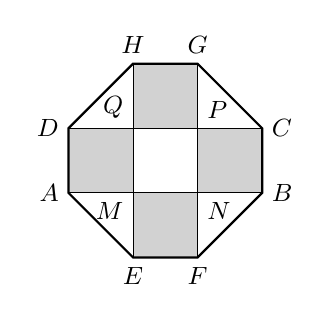
\begin{tikzpicture}[scale=0.82, every node/.style={font=\small}]
  \fill[gray!35] (-1.5,-0.5) rectangle (1.5,0.5);
  \fill[gray!35] (-0.5,-1.5) rectangle (0.5,1.5);
  % 中心正方形 MNPQ 原卷不涂阴影，照原卷留白：
  \fill[white] (-0.5,-0.5) rectangle (0.5,0.5);
  \draw[thick] (-1.5,0.5)--(-0.5,1.5)--(0.5,1.5)--(1.5,0.5)--(1.5,-0.5)--(0.5,-1.5)--(-0.5,-1.5)--(-1.5,-0.5)--cycle;
  \draw (-1.5,-0.5) rectangle (1.5,0.5);
  \draw (-0.5,-1.5) rectangle (0.5,1.5);
  \node[left] at (-1.5,0.5) {$D$};
  \node[left] at (-1.5,-0.5) {$A$};
  \node[right] at (1.5,0.5) {$C$};
  \node[right] at (1.5,-0.5) {$B$};
  \node[above] at (-0.5,1.5) {$H$};
  \node[above] at (0.5,1.5) {$G$};
  \node[below] at (-0.5,-1.5) {$E$};
  \node[below] at (0.5,-1.5) {$F$};
  \node[below left] at (-0.5,-0.5) {$M$};
  \node[below right] at (0.5,-0.5) {$N$};
  \node[above right] at (0.5,0.5) {$P$};
  \node[above left] at (-0.5,0.5) {$Q$};
\end{tikzpicture}
\end{center}

\begin{enumerate}[label=(\arabic*)]
\item 设 $DQ$ 长为 $y$（单位：m），用 $x$ 表示 $y$，并求出 $x$ 的取值范围；
\item $AD$ 取何值时可使总造价最低，并求出最低造价.
\end{enumerate}

\ifanswer
\solbegin
\stepm{(1)}{设 $AD=x\text{m}$（$x>0$），$DQ=y\text{m}$（$y>0$），}
\step{因为十字形区域总面积为 $200\text{m}^2$，所以 $4xy+x^2=200$，}
\step{解得 $y=\dfrac{200-x^2}{4x}=\dfrac{50}{x}-\dfrac{x}{4}$，}
\step{因为 $x>0$，$y>0$，所以 $y=\dfrac{200-x^2}{4x}>0$，解得 $0<x<10\sqrt2$，}
\step{所以 $y=\dfrac{50}{x}-\dfrac{x}{4}$，$0<x<10\sqrt2$；}
\stepm{(2)}{中心正方形 $MNPQ$ 区域，造价为 $2100$ 元$/\text{m}^2$，}
\step{中心正方形 $MNPQ$ 面积为 $S_1=x^2$，造价为 $W_1=2100\times S_1=2100x^2$；}
\step{周围四个矩形区域（图中阴影部分）铺设透水地砖，造价为 $105$ 元$/\text{m}^2$，}
\step{四个矩形的总面积为 $S_2=4xy=4x\left(\dfrac{50}{x}-\dfrac{x}{4}\right)=200-x^2$，}
\step{造价为 $W_2=105\times S_2=105(200-x^2)=21000-105x^2$；}
\step{四个三角形区域种植耐旱固碳植物，助力碳中和，造价为 $40$ 元$/\text{m}^2$，}
\step{四个三角形的总面积为 $S_3=4\times\dfrac12y^2=2\left(\dfrac{50}{x}-\dfrac{x}{4}\right)^2
=\dfrac{5000}{x^2}-50+\dfrac{x^2}{8}$，}
\step{造价为 $W_3=40\times S_3=40\left(\dfrac{5000}{x^2}-50+\dfrac{x^2}{8}\right)
=\dfrac{200000}{x^2}-2000+5x^2$；}
\step{设总造价为 $W$（单位：元），}
\step{则总造价为 $W=W_1+W_2+W_3$}
\step{$=2100x^2+21000-105x^2+\dfrac{200000}{x^2}-2000+5x^2$}
\step{$=2000x^2+\dfrac{200000}{x^2}+19000$，}
\step{又 $2000x^2+\dfrac{200000}{x^2}\geqslant2\sqrt{2000x^2\times\dfrac{200000}{x^2}}=2\times20000=40000$，}
\step{当且仅当 $2000x^2=\dfrac{200000}{x^2}$，即 $x=\sqrt{10}$（在 $x$ 的范围内）时取等号，}
\step{所以 $W=2000x^2+\dfrac{200000}{x^2}+19000\geqslant59000$，当 $x=\sqrt{10}$ 时取等号，}
\step{故当 $AD$ 的长为 $\sqrt{10}$ 时，总造价最低，为 $59000$ 元.}
\solend

\fi

\ansspace[8]

\item 对于实数 $a$、$b$、$c$，若 $|a-c|<|b-c|$，则称 $a$ 比 $b$ 更接近于 $c$. 现已知 $p$、$q$ 都是正有理数.

\begin{enumerate}[label=(\arabic*)]
\item 证明：$\sqrt3$ 必在 $\dfrac pq$ 和 $\dfrac{p+3q}{p+q}$ 之间；
\item 试问 $\dfrac pq$ 和 $\dfrac{p+3q}{p+q}$ 这两个数，哪一个更接近于 $\sqrt3$？说明你的理由；
\item 请你再写出一个有理数，使得它的值比 $\dfrac pq$ 和 $\dfrac{p+3q}{p+q}$ 的值更接近于 $\sqrt3$，并说明你的理由.
\end{enumerate}

\ifanswer
\solbegin
\stepm{(1)}{设 $a=\dfrac pq$（$a$ 为正有理数），则需证 $\sqrt3$ 在 $a$ 和 $\dfrac{a+3}{a+1}$（即 $\dfrac{p+3q}{p+q}$）之间.}
\step{当 $a>\sqrt3$ 时，计算 $a-\dfrac{a+3}{a+1}$ 得 $a-\dfrac{a+3}{a+1}=\dfrac{a(a+1)-(a+3)}{a+1}=\dfrac{a^2-3}{a+1}$，}
\step{$a>\sqrt3$，则 $a^2-3>0$，故 $a>\dfrac{a+3}{a+1}$；}
\step{再计算 $\dfrac{a+3}{a+1}-\sqrt3$ 得 $\dfrac{a+3}{a+1}-\sqrt3=\dfrac{(1-\sqrt3)(a-\sqrt3)}{a+1}$，}
\step{$1-\sqrt3<0$，$a-\sqrt3>0$，$a+1>0$，}
\step{故 $\dfrac{a+3}{a+1}-\sqrt3<0$，即 $\dfrac{a+3}{a+1}<\sqrt3$，从而 $\dfrac{a+3}{a+1}<\sqrt3<a$；}
\step{当 $a<\sqrt3$ 时，同理可得 $a<\dfrac{a+3}{a+1}$ 且 $\dfrac{a+3}{a+1}>\sqrt3$，即 $a<\sqrt3<\dfrac{a+3}{a+1}$，}
\step{综上，$\sqrt3$ 必在 $\dfrac pq$ 和 $\dfrac{p+3q}{p+q}$ 之间；}
\stepm{(2)}{设 $a=\dfrac pq$，$b=\dfrac{p+3q}{p+q}=\dfrac{a+3}{a+1}$，比较 $|a-\sqrt3|$ 与 $|b-\sqrt3|$，}
\step{由（1）得 $(a-\sqrt3)(b-\sqrt3)<0$，}
\step{$\dfrac{|b-\sqrt3|}{|a-\sqrt3|}
=\left|\dfrac{b-\sqrt3}{a-\sqrt3}\right|
=\dfrac{\left|\dfrac{(1-\sqrt3)(a-\sqrt3)}{a+1}\right|}{|a-\sqrt3|}
=\dfrac{\sqrt3-1}{a+1}$，}
\step{$a>0$，$a+1>1$，$\sqrt3-1<1$，故 $\dfrac{\sqrt3-1}{a+1}<1$，即 $|b-\sqrt3|<|a-\sqrt3|$，}
\step{即 $\dfrac{p+3q}{p+q}$ 比 $\dfrac pq$ 更接近于 $\sqrt3$；}
\stepm{(3)}{$\dfrac{2p+3q}{p+2q}$，理由：}
\step{设 $b=\dfrac{p+3q}{p+q}$，新数 $c=\dfrac{b+3}{b+1}=\dfrac{2p+3q}{p+2q}$，}
\step{由（1）得 $(b-\sqrt3)(c-\sqrt3)<0$，}
\step{$c-\sqrt3=\dfrac{b+3}{b+1}-\sqrt3=\dfrac{(1-\sqrt3)(b-\sqrt3)}{b+1}$，}
\step{则 $\dfrac{|c-\sqrt3|}{|b-\sqrt3|}
=\left|\dfrac{c-\sqrt3}{b-\sqrt3}\right|
=\dfrac{\left|\dfrac{(1-\sqrt3)(b-\sqrt3)}{b+1}\right|}{|b-\sqrt3|}
=\dfrac{\sqrt3-1}{b+1}$，}
\step{$b>0$，$b+1>1$，$0<\sqrt3-1<1$，故 $\dfrac{\sqrt3-1}{b+1}<1$，即 $|c-\sqrt3|<|b-\sqrt3|$，}
\step{即 $\dfrac{2p+3q}{p+2q}$ 比 $\dfrac{p+3q}{p+q}$ 更接近于 $\sqrt3$，故 $c$ 更接近 $\sqrt3$.}
\solend

\fi

\ansspace*[10]

\end{enumerate}

\end{document}
"
% 紧凑版：xelatex "\def\iscompact{1}% 高一45_交附闵行_国庆作业2.tex
%   —— 高一上数学“2026-2027 年交附闵行高一上国庆作业 2”（试卷版/答案版）
% 试卷版：xelatex 高一45_交附闵行_国庆作业2.tex
% 答案版：xelatex "\def\isanswer{1}\input{高一45_交附闵行_国庆作业2.tex}"
% 紧凑版：xelatex "\def\iscompact{1}\input{高一45_交附闵行_国庆作业2.tex}"
%
% 原始材料是微信公众号图文（公众号“魔都数学加油站”，作者“破晓”，2026-10-02 17:56 发布，
% 连载“27学年高一45”，原文标题“27学年高一45——2026-2027年上海市交附闵行高一上国庆作业2”，
% https://mp.weixin.qq.com/s/1xdCtzH-3Il0jJrz3saiPA），正文为 10 张 PNG 页。
% 第 01—06、09 页为 4762×6735；第 07、08、10 页为 2560×3620（同一篇各页原图分辨率不一致）。
% 原文本身是一份讲评版：第 3—21 题均照原卷保留题目与题下解析；第 13 题原卷把答案 C 印在括号中。
% 题目、选项、答案与解析均照原卷录入，未改内容；卷面的粉色斜水印及页脚不录入。
%
% 卷首标题：原卷印作“2026-2027 年交附闵行高一上国庆作业 2”（公众号标题里的“上海市”
% 三字卷面标题行没有，本稿照卷面），年份区间按全稿惯例排 en dash，前缀照原卷保留“年”。
%
% 与原卷的排版差异：
%   ① 原卷印有“一、填空题”“二、选择题”“三、解答题”三节标题，本稿照原卷分节，
%      只把标题改排成全稿统一的“大节标题”样式；
%   ② 第 13 题原卷在题干括号内直接印答案 C，本稿按全稿样式将括号留空、答案移入答案版的 \ans{}；
%   ③ 原卷填空横线及选择题答案括号均按全稿样式排版，填空横线统一用 \blankline[4.4em]；
%   ④ 原卷第 20 题配有十字形广场示意图，本稿在源码中用 TikZ 重绘，图中区域、边界及点名照原卷。
%   ⑤ 原卷未印副标题，本稿按本卷实际涉及的知识模块补出“集合与常用逻辑用语、不等式”。
%
% 原卷存疑/错误（均照抄原卷、未改，见对应题目处上方注释）：
%   ① 第 11 题解析原卷印"所以 p=3+9=12，又 12,15∉A，所以 12,15∉B"，与 A∪\overline{B} 的条件
%      及后文 B 的根为 6、9 均一致，无矛盾，本稿照录（早前记录的"∈B／前后矛盾"系本稿误读）；
%   ② 第 15 题题干与解析均按原卷印 ac<0，解析"因为 a<b<c，且 ac<0，所以 a<0，c>0"与题设一致，
%      无矛盾（早前记录的"abc<0／解析冲突"系本稿误读题干所致）；本稿照录原卷答案与解析。
%   ③ 第 20 题原卷各数（造价 2100 元/m^2、W_1=2100x^2、合并式 2000x^2+200000/x^2+19000、
%      末句 59000 元）经复核自洽，无矛盾（早前记录的"W_1=200x^2／末句 5900 元"系本稿误录）；本稿照录。
%   ④ 第 18(2) 题 a=-1 时 A=B=(-1,1)，不满足“B 是 A 的真子集”，故原解析给出的 a≤-1 应为 a<-1；
%   ⑤ 第 19(2) 题原卷用"{c|0<c<1}∩{c|c<-2√3/3 或 c>2√3/3}=∅"论证"不等式①、②中至多有一个恒成立"，
%      论证成立（早前记录的"区间并集留有间隙"系本稿误录解析所致）；本稿照录原卷。
%
\documentclass[a4paper,11pt]{article}
\usepackage{common}

\begin{document}

\examtitlest[3]{2026--2027 年交附闵行高一上国庆作业 2}{集合与常用逻辑用语、不等式}

\bigsec{一、填空题}

\begin{enumerate}
\setcounter{enumi}{2}

\item 满足 $A\cup\{-1,1\}=\{-1,0,1\}$ 的集合 $A$ 共有 \blankline[4.4em] 个.

\ifanswer
\solbegin
\step{集合可能为 $\{0\}$、$\{0,1\}$、$\{0,-1\}$、$\{0,1,-1\}$，共有 $4$ 个.}
\solend

\fi

\item 设 $x\in\R$，则“$x+\dfrac1x>2$”是“$x\neq1$”的 \blankline[4.4em] 条件.

\ifanswer
\solbegin
\step{$x+\dfrac1x>2\Longleftrightarrow x>0$ 且 $x\neq1$，故为充分不必要条件.}
\solend

\fi

\item 已知集合 $A=\{x\mid|x-1|<a\}$，$B=\{-4,3\}$，若 $A\cap B=\varnothing$，则 $a$ 的最大值为 \blankline[4.4em].

\ifanswer
\solbegin
\step{$A=\{x\mid -a<x-1<a\}=\{x\mid1-a<x<1+a\}$，$B=\{-4,3\}$，且 $A\cap B=\varnothing$，}
\step{$A=\varnothing$ 时，$1-a\geqslant1+a$，解得 $a\leqslant0$，满足 $A\cap B=\varnothing$；}
\step{若 $-4\in A$，则 $1-a<-4<1+a$，解得 $a>5$；}
\step{若 $3\in A$，则 $1-a<3<1+a$，解得 $a>2$，}
\step{因为 $A\cap B=\varnothing$，所以 $-4\notin A$ 且 $3\notin A$，所以 $a\leqslant5$ 且 $a\leqslant2$，所以 $a\leqslant2$，}
\step{综上，$a$ 的最大值为 $2$.}
\solend

\fi

\item 设 $x\in\R$，方程 $|x-1|+|2x-1|=|3x-2|$ 的解集为 \blankline[4.4em].

\ifanswer
\solbegin
\step{因为 $|x-1|+|2x-1|\geqslant|(x-1)+(2x-1)|=|3x-2|$，}
\step{当且仅当 $(x-1)(2x-1)\geqslant0$，解得 $x\leqslant\dfrac12$ 或 $x\geqslant1$，}
\step{故方程 $|x-1|+|2x-1|=|3x-2|$ 的解集为 $\left(-\infty,\dfrac12\right]\cup[1,+\infty)$.}
\solend

\fi

\item 已知 $a$、$b\in\R$，且 $3a+2b=1$，则 $8^a+4^b$ 最小值为 \blankline[4.4em].

\ifanswer
\solbegin
% 注：原卷本行与上行均作“$8^a+4^b$ 最小值为”，“最小值”前无“的”，原卷如此，照录未改。
\step{因为 $3a+2b=1$，所以 $8^a+4^b=2^{3a}+2^{2b}\geqslant2\sqrt{2^{3a+2b}}=2\sqrt2$，}
\step{当且仅当 $3a=2b$ 时取等号，故 $8^a+4^b$ 最小值为 $2\sqrt2$.}
\solend

\fi

\item 已知 $a>0$，$b>0$，且 $a+2b+ab=30$，则 $2a+b$ 的最小值为 \blankline[4.4em].

\ifanswer
\solbegin
\step{由 $a+2b+ab=30$，得 $(a+2)(b+1)=32$.}
\step{因为 $a>0$，$b>0$，所以 $a+2>0$，$b+1>0$，}
\step{所以 $2a+b=2(a+2)+(b+1)-5\geqslant2\sqrt{2\times32}-5=11$，}
\step{当且仅当 $2(a+2)=(b+1)$，即 $a=2$，$b=7$ 时取等号，}
\step{所以 $2a+b$ 的最小值为 $11$.}
\solend

\fi

\item 已知 $A=\{x\mid x^2+px+1=0\}$，$M=\{x\mid x>0\}$，若 $A\cap M=\varnothing$，则实数 $p$ 的取值范围为 \blankline[4.4em].

\ifanswer
\solbegin
\step{①当 $A=\varnothing$ 时，$\Delta=p^2-4<0$，所以 $-2<p<2$，此时满足 $A\cap M=\varnothing$；}
\step{②当 $A\neq\varnothing$ 时，$\Delta=p^2-4\geqslant0$，$p\geqslant2$ 或 $p\leqslant-2$，}
\step{因为 $M=\{x\mid x>0\}$，$A\cap M=\varnothing$，由韦达定理得 $\begin{cases}-p\leqslant0\\1>0\end{cases}$，解得 $p\geqslant0$，}
\step{所以 $p\geqslant2$，}
\step{由①②综合得 $p>-2$，故实数 $p$ 的取值范围为 $(-2,+\infty)$.}
\solend

\fi

\item 已知集合 $A=[t,t+1]\cup[t+3,t+6]$，其中 $t>0$. 若存在正数 $\lambda$，使得对任意 $a\in A$，都有 $\dfrac{\lambda}{a}\in A$，则 $t$ 的取值集合为 \blankline[4.4em].

\ifanswer
\solbegin
\step{因为 $0\notin A$，$t>0$，所以 $a\in[t,t+1]\cup[t+3,t+6]$，}
\step{则 $\dfrac1a\in\left[\dfrac1{t+6},\dfrac1{t+3}\right]\cup\left[\dfrac1{t+1},\dfrac1t\right]$，}
\step{又因为 $\lambda>0$，所以 $\dfrac{\lambda}{a}\in\left[\dfrac{\lambda}{t+6},\dfrac{\lambda}{t+3}\right]\cup\left[\dfrac{\lambda}{t+1},\dfrac{\lambda}{t}\right]$，}
\step{因为 $\dfrac{\lambda}{a}\in A$，所以 $\begin{cases}\dfrac{\lambda}{t+6}\geqslant t\\[3pt]\dfrac{\lambda}{t+3}\leqslant t+1\end{cases}$ 且 $\begin{cases}\dfrac{\lambda}{t+1}\geqslant t+3\\[3pt]\dfrac{\lambda}{t}\leqslant t+6\end{cases}$，}
% 注：原卷本行两个不等式组印作“$t(t+6)\leqslant\lambda\leqslant t(t+6)$”与
%     “$(t+1)(t+3)\leqslant\lambda\leqslant(t+1)(t+3)$”（两侧同式），与上行两式推导不合，系原卷笔误；
%     原卷如此，照录未改。
\step{得 $\begin{cases}t(t+6)\leqslant\lambda\leqslant t(t+6)\\[3pt](t+1)(t+3)\leqslant\lambda\leqslant(t+1)(t+3)\end{cases}$，所以 $\lambda=t(t+6)=(t+1)(t+3)$，}
\step{解得 $t=\dfrac32$，取值集合为 $\left\{\dfrac32\right\}$.}
\solend

\fi

\item 已知全集 $U=\{x\mid x=3n,1\leqslant n\leqslant5\ \text{且}\ n\in\N\}$，$A=\{x\mid x^2-px+27=0,p\in\N\}$，
$B=\{x\mid x^2-15x+q=0,q\in\N\}$，且 $A\cup\overline{B}=\{3,9,12,15\}$，则 $p+q$ 的值为 \blankline[4.4em].

\ifanswer
\solbegin
\step{因为全集 $U=\{3,6,9,12,15\}$，$A\cup\overline{B}=\{3,9,12,15\}$，}
\step{所以 $3$、$9$、$12$、$15$ 中可能有两个属于 $A$，}
\step{因为 $A$ 中的方程 $x^2-px+27=0$ 中，两根之积 $x_1x_2=27$，所以 $3$、$9\in A$，}
\step{所以 $p=3+9=12$，又 $12$、$15\notin A$，所以 $12$、$15\notin B$，}
\step{因为 $B$ 中的方程 $x^2-15x+q=0$ 中，两根之和 $x_3+x_4=15$，所以 $6$、$9\in B$，}
\step{则 $q=6\times9=54$，所以 $p+q=66$.}
\solend

\fi

\item 若关于 $x$ 的不等式 $|x-2k|+|x-3k|<4k$ 共有 $2025$ 个整数解，则实数 $k$ 的取值范围为 \blankline[4.4em].

\ifanswer
\solbegin
\step{显然 $k>0$，由 $|x-2k|+|x-3k|<4k$，得 $\dfrac{k}{2}<x<\dfrac{9k}{2}$，}
\step{因为该不等式共有 $2025$ 个整数解，所以 $2024<\dfrac{9k}{2}-\dfrac{k}{2}\leqslant2026$，}
\step{解得 $506<k\leqslant506.5$，}
\step{由 $\dfrac{k}{2}\in(253,253.25]$，得这 $2025$ 个整数解只能为 $254,255,256,\cdots,2278$，}
\step{所以 $2278<\dfrac{9k}{2}\leqslant2279$，解得 $506\dfrac29<k\leqslant506\dfrac49$，结合 $506<k\leqslant506.5$，}
\step{得 $k$ 的取值范围是 $\left(506\dfrac29,506\dfrac49\right]$.}
\solend

\fi

\end{enumerate}

\bigsec{二、选择题}

\begin{enumerate}
\setcounter{enumi}{12}

\item 已知 $a,b\in\R$，且 $ab\neq0$，则下列结论恒成立的是\mbox{（\quad）}

\keepwithprev
A. $a+b\geqslant2\sqrt{ab}$\qquad
B. $\left(\dfrac{a+b}{2}\right)^2>ab$\qquad
C. $\left|\dfrac ab+\dfrac ba\right|\geqslant2$\qquad
D. $a^2+b^2>2ab$

\ans{$C$}

\item 如果 $a^{2025}+b^{2025}=0$，那么一定有\mbox{（\quad）}

\keepwithprev
A. $(|a|+|b|)^{2025}=0$\qquad
B. $(a-b)^{2025}=0$\qquad
C. $(a\cdot b)^{2025}=0$\qquad
D. $(a+b)^{2025}=0$

\ans{$D$}

\ifanswer
\solbegin
\step{由 $a^{2025}+b^{2025}=0$，得 $a^{2025}=-b^{2025}=(-b)^{2025}$，则 $\left(a^{2025}\right)^{\frac{1}{2025}}=\left[(-b)^{2025}\right]^{\frac{1}{2025}}$，}
\step{即 $a=-b$，即 $a+b=0$，故 $(a+b)^{2025}=0$，故 D 符合题意；}
\step{对于 A，若取 $a=1$，$b=-1$，则 $(|a|+|b|)^{2025}=2^{2025}\neq0$，故 A 不合题意；}
\step{对于 B，若取 $a=1$，$b=-1$，则 $(a-b)^{2025}=2^{2025}\neq0$，故 B 不合题意；}
\step{对于 C，若取 $a=1$，$b=-1$，则 $(a\cdot b)^{2025}=(-1)^{2025}=-1\neq0$，故 C 不合题意；}
\step{故选 D.}
\solend

\fi

\item 已知 $a$、$b$、$c$ 满足 $a<b<c$，且 $ac<0$，那么下列各式中一定成立的是\mbox{（\quad）}

\keepwithprev
A. $\dfrac1a>\dfrac1c$\qquad
B. $ab^2<cb^2$\qquad
C. $ac<bc$\qquad
D. $a+c>2b$

\ans{$C$}

\ifanswer
\solbegin
\step{因为 $a<b<c$，且 $ac<0$，所以 $a<0$，$c>0$，}
\step{对于 A，$\dfrac1a<0<\dfrac1c$，故 A 错误；}
\step{对于 B，当 $b=0$ 时，$ab^2=cb^2$，故 B 错误；}
\step{对于 C，$ac<bc$ 可化为 $(a-b)c<0$，因为 $a<b$，所以 $a-b<0$，}
\step{又因为 $c>0$，所以 $(a-b)c<0$，所以 C 正确；}
\step{对于 D，设 $a=-2$，$b=0$，$c=1$，则 $a+c<2b$，故 D 错误.}
\step{故选 C.}
\solend

\fi

\item 对于 $a\in\R$，设集合 $A=\left\{x\mid\dfrac{(x^2-6x+a)(x-1)}{x+a}=0\right\}$，记 $A$ 的所有元素之和为 $S(a)$，
所有元素之积为 $T(a)$，则下列说法中，正确的是\mbox{（\quad）}

\keepwithprev
A. 不存在实数 $a$，使得 $S(a)=6$\qquad
B. 存在实数 $a$，使得 $T(a)=9$

C. 存在无数实数 $a$，使得 $S(a)=7$\qquad
D. 若 $T(a)=3$，则 $a=3$

\ans{$C$}

\ifanswer
\solbegin
\step{要使 $\dfrac{(x^2-6x+a)(x-1)}{x+a}=0$，只需 $(x^2-6x+a)(x-1)=0$ 且 $x+a\neq0$，}
\step{由 $(x^2-6x+a)(x-1)=0$ 得 $x^2-6x+a=0$ 或 $x-1=0$，}
\step{对于一元二次方程 $x^2-6x+a=0$，其判别式 $\Delta=36-4a$，}
\step{当 $\Delta=0$，即 $a=9$ 时，集合 $A=\{1,3\}$，$S(a)=4$，$T(a)=3$；}
\step{当 $\Delta<0$，即 $a>9$ 时，集合 $A=\{1\}$，$S(a)=T(a)=1$；}
\step{当 $\Delta>0$，即 $a<9$ 时，一元二次方程 $x^2-6x+a=0$ 的解为 $x=3\pm\sqrt{9-a}$，}
\step{①当 $a=0$ 时，$x\neq0$，则集合 $A=\{1,6\}$，则 $S(a)=7$，$T(a)=6$，}
\step{②当 $a=-7$ 时，$x\neq7$，则集合 $A=\{-1,1\}$，则 $S(a)=0$，$T(a)=-1$，}
% 注：下一行集合 A 原卷印作 {-1,1}（按 a=-1 代入 x^2-6x-1=0 应得 3±√10，原卷如此，照录未改）。
\step{③当 $a=-1$ 时，$x\neq1$，则集合 $A=\{-1,1\}$，则 $S(a)=6$，$T(a)=-1$，}
\step{④当 $a=5$ 时，$x\neq-5$，则集合 $A=\{1,5\}$，则 $S(a)=6$，$T(a)=5$，}
\step{⑤当 $a\neq5,0,-1,-7$ 时，集合 $A=\{1,3-\sqrt{9-a},3+\sqrt{9-a}\}$，}
\step{则 $S(a)=7$，$T(a)=a$.}
\step{选项 A，当 $a=5$ 时，$S(a)=6$，所以 A 错误；}
\step{选项 B，$T(a)$ 的可能值为 $-1,1,3,5,6,a$（$a<9$），无 $T(a)=9$，所以 B 错误；}
\step{选项 C，当 $a<9$，且 $a\neq5,-1,-7$ 时，$S(a)=7$，有无数个 $a$ 满足，所以 C 正确；}
\step{选项 D，当 $T(a)=3$ 时，有 $a=3$ 和 $a=9$ 满足，所以 D 错误.}
\step{故选 C.}
\solend

\fi

\end{enumerate}

\bigsec{三、解答题}

\begin{enumerate}
\setcounter{enumi}{16}

\item 已知 $a\in\R$，关于 $x$ 的不等式 $|x+1|+|x-1|>a^2-5a+4$.

\begin{enumerate}[label=(\arabic*)]
\item 当 $a=0$ 时，求不等式的解集；
\item 若不等式的解集为 $\R$，求 $a$ 的取值范围.
\end{enumerate}

\ifanswer
\solbegin
\stepm{(1)}{当 $a=0$ 时，不等式为 $|x+1|+|x-1|>4$，}
\step{又 $|x+1|+|x-1|=\begin{cases}2x,&x\geqslant1\\2,&-1<x<1\\-2x,&x\leqslant-1\end{cases}$，}
\step{则 $|x+1|+|x-1|>4$ 的解为 $x>2$ 或 $x<-2$，}
\step{即不等式的解集为 $(-\infty,-2)\cup(2,+\infty)$；}
\stepm{(2)}{不等式 $|x+1|+|x-1|>a^2-5a+4$ 的解集为 $\R$，}
\step{则 $(|x+1|+|x-1|)_{\min}>a^2-5a+4$，}
\step{又 $(|x+1|+|x-1|)_{\min}=2$，当且仅当 $-1\leqslant x\leqslant1$ 时取得，即 $a^2-5a+4<2$，}
\step{即 $a^2-5a+2<0$，即 $\dfrac{5-\sqrt{17}}2<a<\dfrac{5+\sqrt{17}}2$，}
\step{即 $a$ 的取值范围为 $\left(\dfrac{5-\sqrt{17}}2,\dfrac{5+\sqrt{17}}2\right)$.}
\solend

\fi

\ansspace[6]

\item 已知集合 $A=\{x\mid(x-a)(x-a^2)<0\}$，集合 $B=\left\{x\mid\dfrac{2x}{x-1}<1\right\}$，命题 $p:x\in A$，命题 $q:x\in B$.

\begin{enumerate}[label=(\arabic*)]
\item 当实数 $a$ 为何值时，$A=B$；
\item 若 $q$ 是 $p$ 的充分不必要条件，求实数 $a$ 的取值范围.
\end{enumerate}

\ifanswer
\solbegin
\stepm{(1)}{由 $\dfrac{2x}{x-1}<1$ 得 $\dfrac{2x}{x-1}-1=\dfrac{x+1}{x-1}<0$，解得 $-1<x<1$，即 $B=\{x\mid-1<x<1\}$，}
\step{因为 $A=\{x\mid(x-a)(x-a^2)<0\}$，$A=B$，所以 $\begin{cases}a=-1\\a^2=1\end{cases}$，解得 $a=-1$；}
\stepm{(2)}{若 $q$ 是 $p$ 的充分不必要条件，则 $B\subset A$，}
\step{当 $a^2=a$，即 $a=0$ 或 $a=1$ 时，$A=\varnothing$，显然不符合题意；}
\step{当 $a^2>a$，即 $a>1$ 或 $a<0$ 时，$A=(a,a^2)$，则 $\begin{cases}a\leqslant-1\\a^2\geqslant1\\a>1\ \text{或}\ a<0\end{cases}$，}
% 注：a=-1 时 A=(-1,1)=B，不是 B 的真子集；原解析用 B⊂A 但答案含 -1，照录。
\step{前两等号不能同时取得，解得 $a\leqslant-1$；}
\step{当 $a^2<a$，即 $0<a<1$ 时，$A=(a^2,a)$，显然不符合题意，}
\step{故 $a$ 的范围为 $\{a\mid a\leqslant-1\}$.}
\solend

\fi

\ansspace[6]

\item 已知不等式① $x^2+2cx+c>0$，② $x^2+cx+c^2-1>0$，其中 $c$ 是实数.

\begin{enumerate}[label=(\arabic*)]
\item 若 $1$ 是不等式②的一个解，求实数 $c$ 的取值范围；
\item 证明：不等式①、②中至多有一个恒成立.
\end{enumerate}

\ifanswer
\solbegin
\stepm{(1)}{已知不等式① $x^2+2cx+c>0$，② $x^2+cx+c^2-1>0$，}
\step{又 $1$ 是不等式②的一个解，则 $1+c+c^2-1>0$，}
\step{则 $c^2+c>0$，则 $c<-1$ 或 $c>0$，则 $c$ 的取值范围为 $(-\infty,-1)\cup(0,+\infty)$；}
\stepm{(2)}{若不等式①恒成立，则 $\Delta=4c^2-4c<0$，则 $0<c<1$，}
\step{若不等式②恒成立，则 $\Delta=c^2-4(c^2-1)=4-3c^2<0$，}
\step{则 $c<-\dfrac{2\sqrt3}{3}$ 或 $c>\dfrac{2\sqrt3}{3}$，}
\step{又 $\{c\mid 0<c<1\}\cap\left\{c\mid c<-\dfrac{2\sqrt3}{3}\ \text{或}\ c>\dfrac{2\sqrt3}{3}\right\}=\varnothing$，}
\step{则不存在实数 $c$ 使得不等式①、②同时恒成立，}
\step{则不等式①、②中至多有一个恒成立.}
\solend

\fi

\ansspace[6]

\item 为践行“科技强国”战略，某社区计划建造一座融合智慧节能技术的八边形休闲广场，其中两个相同的矩形 $ABCD$ 和 $EFGH$ 构成的十字形区域总面积为 $200\text{m}^2$. 中心正方形 $MNPQ$ 区域将安装国产太阳能光伏板（兼具休憩遮阳功能），造价为 $2100$ 元$/\text{m}^2$；周围四个矩形区域（图中阴影部分）铺设透水地砖，造价为 $105$ 元$/\text{m}^2$；再在四个三角形区域种植耐旱固碳植物，助力碳中和，造价为 $40$ 元$/\text{m}^2$. 设总造价为 $W$（单位：元），$AD=x$（单位：m）.

\begin{center}
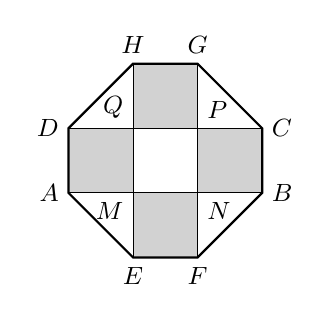
\begin{tikzpicture}[scale=0.82, every node/.style={font=\small}]
  \fill[gray!35] (-1.5,-0.5) rectangle (1.5,0.5);
  \fill[gray!35] (-0.5,-1.5) rectangle (0.5,1.5);
  % 中心正方形 MNPQ 原卷不涂阴影，照原卷留白：
  \fill[white] (-0.5,-0.5) rectangle (0.5,0.5);
  \draw[thick] (-1.5,0.5)--(-0.5,1.5)--(0.5,1.5)--(1.5,0.5)--(1.5,-0.5)--(0.5,-1.5)--(-0.5,-1.5)--(-1.5,-0.5)--cycle;
  \draw (-1.5,-0.5) rectangle (1.5,0.5);
  \draw (-0.5,-1.5) rectangle (0.5,1.5);
  \node[left] at (-1.5,0.5) {$D$};
  \node[left] at (-1.5,-0.5) {$A$};
  \node[right] at (1.5,0.5) {$C$};
  \node[right] at (1.5,-0.5) {$B$};
  \node[above] at (-0.5,1.5) {$H$};
  \node[above] at (0.5,1.5) {$G$};
  \node[below] at (-0.5,-1.5) {$E$};
  \node[below] at (0.5,-1.5) {$F$};
  \node[below left] at (-0.5,-0.5) {$M$};
  \node[below right] at (0.5,-0.5) {$N$};
  \node[above right] at (0.5,0.5) {$P$};
  \node[above left] at (-0.5,0.5) {$Q$};
\end{tikzpicture}
\end{center}

\begin{enumerate}[label=(\arabic*)]
\item 设 $DQ$ 长为 $y$（单位：m），用 $x$ 表示 $y$，并求出 $x$ 的取值范围；
\item $AD$ 取何值时可使总造价最低，并求出最低造价.
\end{enumerate}

\ifanswer
\solbegin
\stepm{(1)}{设 $AD=x\text{m}$（$x>0$），$DQ=y\text{m}$（$y>0$），}
\step{因为十字形区域总面积为 $200\text{m}^2$，所以 $4xy+x^2=200$，}
\step{解得 $y=\dfrac{200-x^2}{4x}=\dfrac{50}{x}-\dfrac{x}{4}$，}
\step{因为 $x>0$，$y>0$，所以 $y=\dfrac{200-x^2}{4x}>0$，解得 $0<x<10\sqrt2$，}
\step{所以 $y=\dfrac{50}{x}-\dfrac{x}{4}$，$0<x<10\sqrt2$；}
\stepm{(2)}{中心正方形 $MNPQ$ 区域，造价为 $2100$ 元$/\text{m}^2$，}
\step{中心正方形 $MNPQ$ 面积为 $S_1=x^2$，造价为 $W_1=2100\times S_1=2100x^2$；}
\step{周围四个矩形区域（图中阴影部分）铺设透水地砖，造价为 $105$ 元$/\text{m}^2$，}
\step{四个矩形的总面积为 $S_2=4xy=4x\left(\dfrac{50}{x}-\dfrac{x}{4}\right)=200-x^2$，}
\step{造价为 $W_2=105\times S_2=105(200-x^2)=21000-105x^2$；}
\step{四个三角形区域种植耐旱固碳植物，助力碳中和，造价为 $40$ 元$/\text{m}^2$，}
\step{四个三角形的总面积为 $S_3=4\times\dfrac12y^2=2\left(\dfrac{50}{x}-\dfrac{x}{4}\right)^2
=\dfrac{5000}{x^2}-50+\dfrac{x^2}{8}$，}
\step{造价为 $W_3=40\times S_3=40\left(\dfrac{5000}{x^2}-50+\dfrac{x^2}{8}\right)
=\dfrac{200000}{x^2}-2000+5x^2$；}
\step{设总造价为 $W$（单位：元），}
\step{则总造价为 $W=W_1+W_2+W_3$}
\step{$=2100x^2+21000-105x^2+\dfrac{200000}{x^2}-2000+5x^2$}
\step{$=2000x^2+\dfrac{200000}{x^2}+19000$，}
\step{又 $2000x^2+\dfrac{200000}{x^2}\geqslant2\sqrt{2000x^2\times\dfrac{200000}{x^2}}=2\times20000=40000$，}
\step{当且仅当 $2000x^2=\dfrac{200000}{x^2}$，即 $x=\sqrt{10}$（在 $x$ 的范围内）时取等号，}
\step{所以 $W=2000x^2+\dfrac{200000}{x^2}+19000\geqslant59000$，当 $x=\sqrt{10}$ 时取等号，}
\step{故当 $AD$ 的长为 $\sqrt{10}$ 时，总造价最低，为 $59000$ 元.}
\solend

\fi

\ansspace[8]

\item 对于实数 $a$、$b$、$c$，若 $|a-c|<|b-c|$，则称 $a$ 比 $b$ 更接近于 $c$. 现已知 $p$、$q$ 都是正有理数.

\begin{enumerate}[label=(\arabic*)]
\item 证明：$\sqrt3$ 必在 $\dfrac pq$ 和 $\dfrac{p+3q}{p+q}$ 之间；
\item 试问 $\dfrac pq$ 和 $\dfrac{p+3q}{p+q}$ 这两个数，哪一个更接近于 $\sqrt3$？说明你的理由；
\item 请你再写出一个有理数，使得它的值比 $\dfrac pq$ 和 $\dfrac{p+3q}{p+q}$ 的值更接近于 $\sqrt3$，并说明你的理由.
\end{enumerate}

\ifanswer
\solbegin
\stepm{(1)}{设 $a=\dfrac pq$（$a$ 为正有理数），则需证 $\sqrt3$ 在 $a$ 和 $\dfrac{a+3}{a+1}$（即 $\dfrac{p+3q}{p+q}$）之间.}
\step{当 $a>\sqrt3$ 时，计算 $a-\dfrac{a+3}{a+1}$ 得 $a-\dfrac{a+3}{a+1}=\dfrac{a(a+1)-(a+3)}{a+1}=\dfrac{a^2-3}{a+1}$，}
\step{$a>\sqrt3$，则 $a^2-3>0$，故 $a>\dfrac{a+3}{a+1}$；}
\step{再计算 $\dfrac{a+3}{a+1}-\sqrt3$ 得 $\dfrac{a+3}{a+1}-\sqrt3=\dfrac{(1-\sqrt3)(a-\sqrt3)}{a+1}$，}
\step{$1-\sqrt3<0$，$a-\sqrt3>0$，$a+1>0$，}
\step{故 $\dfrac{a+3}{a+1}-\sqrt3<0$，即 $\dfrac{a+3}{a+1}<\sqrt3$，从而 $\dfrac{a+3}{a+1}<\sqrt3<a$；}
\step{当 $a<\sqrt3$ 时，同理可得 $a<\dfrac{a+3}{a+1}$ 且 $\dfrac{a+3}{a+1}>\sqrt3$，即 $a<\sqrt3<\dfrac{a+3}{a+1}$，}
\step{综上，$\sqrt3$ 必在 $\dfrac pq$ 和 $\dfrac{p+3q}{p+q}$ 之间；}
\stepm{(2)}{设 $a=\dfrac pq$，$b=\dfrac{p+3q}{p+q}=\dfrac{a+3}{a+1}$，比较 $|a-\sqrt3|$ 与 $|b-\sqrt3|$，}
\step{由（1）得 $(a-\sqrt3)(b-\sqrt3)<0$，}
\step{$\dfrac{|b-\sqrt3|}{|a-\sqrt3|}
=\left|\dfrac{b-\sqrt3}{a-\sqrt3}\right|
=\dfrac{\left|\dfrac{(1-\sqrt3)(a-\sqrt3)}{a+1}\right|}{|a-\sqrt3|}
=\dfrac{\sqrt3-1}{a+1}$，}
\step{$a>0$，$a+1>1$，$\sqrt3-1<1$，故 $\dfrac{\sqrt3-1}{a+1}<1$，即 $|b-\sqrt3|<|a-\sqrt3|$，}
\step{即 $\dfrac{p+3q}{p+q}$ 比 $\dfrac pq$ 更接近于 $\sqrt3$；}
\stepm{(3)}{$\dfrac{2p+3q}{p+2q}$，理由：}
\step{设 $b=\dfrac{p+3q}{p+q}$，新数 $c=\dfrac{b+3}{b+1}=\dfrac{2p+3q}{p+2q}$，}
\step{由（1）得 $(b-\sqrt3)(c-\sqrt3)<0$，}
\step{$c-\sqrt3=\dfrac{b+3}{b+1}-\sqrt3=\dfrac{(1-\sqrt3)(b-\sqrt3)}{b+1}$，}
\step{则 $\dfrac{|c-\sqrt3|}{|b-\sqrt3|}
=\left|\dfrac{c-\sqrt3}{b-\sqrt3}\right|
=\dfrac{\left|\dfrac{(1-\sqrt3)(b-\sqrt3)}{b+1}\right|}{|b-\sqrt3|}
=\dfrac{\sqrt3-1}{b+1}$，}
\step{$b>0$，$b+1>1$，$0<\sqrt3-1<1$，故 $\dfrac{\sqrt3-1}{b+1}<1$，即 $|c-\sqrt3|<|b-\sqrt3|$，}
\step{即 $\dfrac{2p+3q}{p+2q}$ 比 $\dfrac{p+3q}{p+q}$ 更接近于 $\sqrt3$，故 $c$ 更接近 $\sqrt3$.}
\solend

\fi

\ansspace*[10]

\end{enumerate}

\end{document}
"
%
% 原始材料是微信公众号图文（公众号“魔都数学加油站”，作者“破晓”，2026-10-02 17:56 发布，
% 连载“27学年高一45”，原文标题“27学年高一45——2026-2027年上海市交附闵行高一上国庆作业2”，
% https://mp.weixin.qq.com/s/1xdCtzH-3Il0jJrz3saiPA），正文为 10 张 PNG 页。
% 第 01—06、09 页为 4762×6735；第 07、08、10 页为 2560×3620（同一篇各页原图分辨率不一致）。
% 原文本身是一份讲评版：第 3—21 题均照原卷保留题目与题下解析；第 13 题原卷把答案 C 印在括号中。
% 题目、选项、答案与解析均照原卷录入，未改内容；卷面的粉色斜水印及页脚不录入。
%
% 卷首标题：原卷印作“2026-2027 年交附闵行高一上国庆作业 2”（公众号标题里的“上海市”
% 三字卷面标题行没有，本稿照卷面），年份区间按全稿惯例排 en dash，前缀照原卷保留“年”。
%
% 与原卷的排版差异：
%   ① 原卷印有“一、填空题”“二、选择题”“三、解答题”三节标题，本稿照原卷分节，
%      只把标题改排成全稿统一的“大节标题”样式；
%   ② 第 13 题原卷在题干括号内直接印答案 C，本稿按全稿样式将括号留空、答案移入答案版的 \ans{}；
%   ③ 原卷填空横线及选择题答案括号均按全稿样式排版，填空横线统一用 \blankline[4.4em]；
%   ④ 原卷第 20 题配有十字形广场示意图，本稿在源码中用 TikZ 重绘，图中区域、边界及点名照原卷。
%   ⑤ 原卷未印副标题，本稿按本卷实际涉及的知识模块补出“集合与常用逻辑用语、不等式”。
%
% 原卷存疑/错误（均照抄原卷、未改，见对应题目处上方注释）：
%   ① 第 11 题解析原卷印"所以 p=3+9=12，又 12,15∉A，所以 12,15∉B"，与 A∪\overline{B} 的条件
%      及后文 B 的根为 6、9 均一致，无矛盾，本稿照录（早前记录的"∈B／前后矛盾"系本稿误读）；
%   ② 第 15 题题干与解析均按原卷印 ac<0，解析"因为 a<b<c，且 ac<0，所以 a<0，c>0"与题设一致，
%      无矛盾（早前记录的"abc<0／解析冲突"系本稿误读题干所致）；本稿照录原卷答案与解析。
%   ③ 第 20 题原卷各数（造价 2100 元/m^2、W_1=2100x^2、合并式 2000x^2+200000/x^2+19000、
%      末句 59000 元）经复核自洽，无矛盾（早前记录的"W_1=200x^2／末句 5900 元"系本稿误录）；本稿照录。
%   ④ 第 18(2) 题 a=-1 时 A=B=(-1,1)，不满足“B 是 A 的真子集”，故原解析给出的 a≤-1 应为 a<-1；
%   ⑤ 第 19(2) 题原卷用"{c|0<c<1}∩{c|c<-2√3/3 或 c>2√3/3}=∅"论证"不等式①、②中至多有一个恒成立"，
%      论证成立（早前记录的"区间并集留有间隙"系本稿误录解析所致）；本稿照录原卷。
%
\documentclass[a4paper,11pt]{article}
\usepackage{common}

\begin{document}

\examtitlest[3]{2026--2027 年交附闵行高一上国庆作业 2}{集合与常用逻辑用语、不等式}

\bigsec{一、填空题}

\begin{enumerate}
\setcounter{enumi}{2}

\item 满足 $A\cup\{-1,1\}=\{-1,0,1\}$ 的集合 $A$ 共有 \blankline[4.4em] 个.

\ifanswer
\solbegin
\step{集合可能为 $\{0\}$、$\{0,1\}$、$\{0,-1\}$、$\{0,1,-1\}$，共有 $4$ 个.}
\solend

\fi

\item 设 $x\in\R$，则“$x+\dfrac1x>2$”是“$x\neq1$”的 \blankline[4.4em] 条件.

\ifanswer
\solbegin
\step{$x+\dfrac1x>2\Longleftrightarrow x>0$ 且 $x\neq1$，故为充分不必要条件.}
\solend

\fi

\item 已知集合 $A=\{x\mid|x-1|<a\}$，$B=\{-4,3\}$，若 $A\cap B=\varnothing$，则 $a$ 的最大值为 \blankline[4.4em].

\ifanswer
\solbegin
\step{$A=\{x\mid -a<x-1<a\}=\{x\mid1-a<x<1+a\}$，$B=\{-4,3\}$，且 $A\cap B=\varnothing$，}
\step{$A=\varnothing$ 时，$1-a\geqslant1+a$，解得 $a\leqslant0$，满足 $A\cap B=\varnothing$；}
\step{若 $-4\in A$，则 $1-a<-4<1+a$，解得 $a>5$；}
\step{若 $3\in A$，则 $1-a<3<1+a$，解得 $a>2$，}
\step{因为 $A\cap B=\varnothing$，所以 $-4\notin A$ 且 $3\notin A$，所以 $a\leqslant5$ 且 $a\leqslant2$，所以 $a\leqslant2$，}
\step{综上，$a$ 的最大值为 $2$.}
\solend

\fi

\item 设 $x\in\R$，方程 $|x-1|+|2x-1|=|3x-2|$ 的解集为 \blankline[4.4em].

\ifanswer
\solbegin
\step{因为 $|x-1|+|2x-1|\geqslant|(x-1)+(2x-1)|=|3x-2|$，}
\step{当且仅当 $(x-1)(2x-1)\geqslant0$，解得 $x\leqslant\dfrac12$ 或 $x\geqslant1$，}
\step{故方程 $|x-1|+|2x-1|=|3x-2|$ 的解集为 $\left(-\infty,\dfrac12\right]\cup[1,+\infty)$.}
\solend

\fi

\item 已知 $a$、$b\in\R$，且 $3a+2b=1$，则 $8^a+4^b$ 最小值为 \blankline[4.4em].

\ifanswer
\solbegin
% 注：原卷本行与上行均作“$8^a+4^b$ 最小值为”，“最小值”前无“的”，原卷如此，照录未改。
\step{因为 $3a+2b=1$，所以 $8^a+4^b=2^{3a}+2^{2b}\geqslant2\sqrt{2^{3a+2b}}=2\sqrt2$，}
\step{当且仅当 $3a=2b$ 时取等号，故 $8^a+4^b$ 最小值为 $2\sqrt2$.}
\solend

\fi

\item 已知 $a>0$，$b>0$，且 $a+2b+ab=30$，则 $2a+b$ 的最小值为 \blankline[4.4em].

\ifanswer
\solbegin
\step{由 $a+2b+ab=30$，得 $(a+2)(b+1)=32$.}
\step{因为 $a>0$，$b>0$，所以 $a+2>0$，$b+1>0$，}
\step{所以 $2a+b=2(a+2)+(b+1)-5\geqslant2\sqrt{2\times32}-5=11$，}
\step{当且仅当 $2(a+2)=(b+1)$，即 $a=2$，$b=7$ 时取等号，}
\step{所以 $2a+b$ 的最小值为 $11$.}
\solend

\fi

\item 已知 $A=\{x\mid x^2+px+1=0\}$，$M=\{x\mid x>0\}$，若 $A\cap M=\varnothing$，则实数 $p$ 的取值范围为 \blankline[4.4em].

\ifanswer
\solbegin
\step{①当 $A=\varnothing$ 时，$\Delta=p^2-4<0$，所以 $-2<p<2$，此时满足 $A\cap M=\varnothing$；}
\step{②当 $A\neq\varnothing$ 时，$\Delta=p^2-4\geqslant0$，$p\geqslant2$ 或 $p\leqslant-2$，}
\step{因为 $M=\{x\mid x>0\}$，$A\cap M=\varnothing$，由韦达定理得 $\begin{cases}-p\leqslant0\\1>0\end{cases}$，解得 $p\geqslant0$，}
\step{所以 $p\geqslant2$，}
\step{由①②综合得 $p>-2$，故实数 $p$ 的取值范围为 $(-2,+\infty)$.}
\solend

\fi

\item 已知集合 $A=[t,t+1]\cup[t+3,t+6]$，其中 $t>0$. 若存在正数 $\lambda$，使得对任意 $a\in A$，都有 $\dfrac{\lambda}{a}\in A$，则 $t$ 的取值集合为 \blankline[4.4em].

\ifanswer
\solbegin
\step{因为 $0\notin A$，$t>0$，所以 $a\in[t,t+1]\cup[t+3,t+6]$，}
\step{则 $\dfrac1a\in\left[\dfrac1{t+6},\dfrac1{t+3}\right]\cup\left[\dfrac1{t+1},\dfrac1t\right]$，}
\step{又因为 $\lambda>0$，所以 $\dfrac{\lambda}{a}\in\left[\dfrac{\lambda}{t+6},\dfrac{\lambda}{t+3}\right]\cup\left[\dfrac{\lambda}{t+1},\dfrac{\lambda}{t}\right]$，}
\step{因为 $\dfrac{\lambda}{a}\in A$，所以 $\begin{cases}\dfrac{\lambda}{t+6}\geqslant t\\[3pt]\dfrac{\lambda}{t+3}\leqslant t+1\end{cases}$ 且 $\begin{cases}\dfrac{\lambda}{t+1}\geqslant t+3\\[3pt]\dfrac{\lambda}{t}\leqslant t+6\end{cases}$，}
% 注：原卷本行两个不等式组印作“$t(t+6)\leqslant\lambda\leqslant t(t+6)$”与
%     “$(t+1)(t+3)\leqslant\lambda\leqslant(t+1)(t+3)$”（两侧同式），与上行两式推导不合，系原卷笔误；
%     原卷如此，照录未改。
\step{得 $\begin{cases}t(t+6)\leqslant\lambda\leqslant t(t+6)\\[3pt](t+1)(t+3)\leqslant\lambda\leqslant(t+1)(t+3)\end{cases}$，所以 $\lambda=t(t+6)=(t+1)(t+3)$，}
\step{解得 $t=\dfrac32$，取值集合为 $\left\{\dfrac32\right\}$.}
\solend

\fi

\item 已知全集 $U=\{x\mid x=3n,1\leqslant n\leqslant5\ \text{且}\ n\in\N\}$，$A=\{x\mid x^2-px+27=0,p\in\N\}$，
$B=\{x\mid x^2-15x+q=0,q\in\N\}$，且 $A\cup\overline{B}=\{3,9,12,15\}$，则 $p+q$ 的值为 \blankline[4.4em].

\ifanswer
\solbegin
\step{因为全集 $U=\{3,6,9,12,15\}$，$A\cup\overline{B}=\{3,9,12,15\}$，}
\step{所以 $3$、$9$、$12$、$15$ 中可能有两个属于 $A$，}
\step{因为 $A$ 中的方程 $x^2-px+27=0$ 中，两根之积 $x_1x_2=27$，所以 $3$、$9\in A$，}
\step{所以 $p=3+9=12$，又 $12$、$15\notin A$，所以 $12$、$15\notin B$，}
\step{因为 $B$ 中的方程 $x^2-15x+q=0$ 中，两根之和 $x_3+x_4=15$，所以 $6$、$9\in B$，}
\step{则 $q=6\times9=54$，所以 $p+q=66$.}
\solend

\fi

\item 若关于 $x$ 的不等式 $|x-2k|+|x-3k|<4k$ 共有 $2025$ 个整数解，则实数 $k$ 的取值范围为 \blankline[4.4em].

\ifanswer
\solbegin
\step{显然 $k>0$，由 $|x-2k|+|x-3k|<4k$，得 $\dfrac{k}{2}<x<\dfrac{9k}{2}$，}
\step{因为该不等式共有 $2025$ 个整数解，所以 $2024<\dfrac{9k}{2}-\dfrac{k}{2}\leqslant2026$，}
\step{解得 $506<k\leqslant506.5$，}
\step{由 $\dfrac{k}{2}\in(253,253.25]$，得这 $2025$ 个整数解只能为 $254,255,256,\cdots,2278$，}
\step{所以 $2278<\dfrac{9k}{2}\leqslant2279$，解得 $506\dfrac29<k\leqslant506\dfrac49$，结合 $506<k\leqslant506.5$，}
\step{得 $k$ 的取值范围是 $\left(506\dfrac29,506\dfrac49\right]$.}
\solend

\fi

\end{enumerate}

\bigsec{二、选择题}

\begin{enumerate}
\setcounter{enumi}{12}

\item 已知 $a,b\in\R$，且 $ab\neq0$，则下列结论恒成立的是\mbox{（\quad）}

\keepwithprev
A. $a+b\geqslant2\sqrt{ab}$\qquad
B. $\left(\dfrac{a+b}{2}\right)^2>ab$\qquad
C. $\left|\dfrac ab+\dfrac ba\right|\geqslant2$\qquad
D. $a^2+b^2>2ab$

\ans{$C$}

\item 如果 $a^{2025}+b^{2025}=0$，那么一定有\mbox{（\quad）}

\keepwithprev
A. $(|a|+|b|)^{2025}=0$\qquad
B. $(a-b)^{2025}=0$\qquad
C. $(a\cdot b)^{2025}=0$\qquad
D. $(a+b)^{2025}=0$

\ans{$D$}

\ifanswer
\solbegin
\step{由 $a^{2025}+b^{2025}=0$，得 $a^{2025}=-b^{2025}=(-b)^{2025}$，则 $\left(a^{2025}\right)^{\frac{1}{2025}}=\left[(-b)^{2025}\right]^{\frac{1}{2025}}$，}
\step{即 $a=-b$，即 $a+b=0$，故 $(a+b)^{2025}=0$，故 D 符合题意；}
\step{对于 A，若取 $a=1$，$b=-1$，则 $(|a|+|b|)^{2025}=2^{2025}\neq0$，故 A 不合题意；}
\step{对于 B，若取 $a=1$，$b=-1$，则 $(a-b)^{2025}=2^{2025}\neq0$，故 B 不合题意；}
\step{对于 C，若取 $a=1$，$b=-1$，则 $(a\cdot b)^{2025}=(-1)^{2025}=-1\neq0$，故 C 不合题意；}
\step{故选 D.}
\solend

\fi

\item 已知 $a$、$b$、$c$ 满足 $a<b<c$，且 $ac<0$，那么下列各式中一定成立的是\mbox{（\quad）}

\keepwithprev
A. $\dfrac1a>\dfrac1c$\qquad
B. $ab^2<cb^2$\qquad
C. $ac<bc$\qquad
D. $a+c>2b$

\ans{$C$}

\ifanswer
\solbegin
\step{因为 $a<b<c$，且 $ac<0$，所以 $a<0$，$c>0$，}
\step{对于 A，$\dfrac1a<0<\dfrac1c$，故 A 错误；}
\step{对于 B，当 $b=0$ 时，$ab^2=cb^2$，故 B 错误；}
\step{对于 C，$ac<bc$ 可化为 $(a-b)c<0$，因为 $a<b$，所以 $a-b<0$，}
\step{又因为 $c>0$，所以 $(a-b)c<0$，所以 C 正确；}
\step{对于 D，设 $a=-2$，$b=0$，$c=1$，则 $a+c<2b$，故 D 错误.}
\step{故选 C.}
\solend

\fi

\item 对于 $a\in\R$，设集合 $A=\left\{x\mid\dfrac{(x^2-6x+a)(x-1)}{x+a}=0\right\}$，记 $A$ 的所有元素之和为 $S(a)$，
所有元素之积为 $T(a)$，则下列说法中，正确的是\mbox{（\quad）}

\keepwithprev
A. 不存在实数 $a$，使得 $S(a)=6$\qquad
B. 存在实数 $a$，使得 $T(a)=9$

C. 存在无数实数 $a$，使得 $S(a)=7$\qquad
D. 若 $T(a)=3$，则 $a=3$

\ans{$C$}

\ifanswer
\solbegin
\step{要使 $\dfrac{(x^2-6x+a)(x-1)}{x+a}=0$，只需 $(x^2-6x+a)(x-1)=0$ 且 $x+a\neq0$，}
\step{由 $(x^2-6x+a)(x-1)=0$ 得 $x^2-6x+a=0$ 或 $x-1=0$，}
\step{对于一元二次方程 $x^2-6x+a=0$，其判别式 $\Delta=36-4a$，}
\step{当 $\Delta=0$，即 $a=9$ 时，集合 $A=\{1,3\}$，$S(a)=4$，$T(a)=3$；}
\step{当 $\Delta<0$，即 $a>9$ 时，集合 $A=\{1\}$，$S(a)=T(a)=1$；}
\step{当 $\Delta>0$，即 $a<9$ 时，一元二次方程 $x^2-6x+a=0$ 的解为 $x=3\pm\sqrt{9-a}$，}
\step{①当 $a=0$ 时，$x\neq0$，则集合 $A=\{1,6\}$，则 $S(a)=7$，$T(a)=6$，}
\step{②当 $a=-7$ 时，$x\neq7$，则集合 $A=\{-1,1\}$，则 $S(a)=0$，$T(a)=-1$，}
% 注：下一行集合 A 原卷印作 {-1,1}（按 a=-1 代入 x^2-6x-1=0 应得 3±√10，原卷如此，照录未改）。
\step{③当 $a=-1$ 时，$x\neq1$，则集合 $A=\{-1,1\}$，则 $S(a)=6$，$T(a)=-1$，}
\step{④当 $a=5$ 时，$x\neq-5$，则集合 $A=\{1,5\}$，则 $S(a)=6$，$T(a)=5$，}
\step{⑤当 $a\neq5,0,-1,-7$ 时，集合 $A=\{1,3-\sqrt{9-a},3+\sqrt{9-a}\}$，}
\step{则 $S(a)=7$，$T(a)=a$.}
\step{选项 A，当 $a=5$ 时，$S(a)=6$，所以 A 错误；}
\step{选项 B，$T(a)$ 的可能值为 $-1,1,3,5,6,a$（$a<9$），无 $T(a)=9$，所以 B 错误；}
\step{选项 C，当 $a<9$，且 $a\neq5,-1,-7$ 时，$S(a)=7$，有无数个 $a$ 满足，所以 C 正确；}
\step{选项 D，当 $T(a)=3$ 时，有 $a=3$ 和 $a=9$ 满足，所以 D 错误.}
\step{故选 C.}
\solend

\fi

\end{enumerate}

\bigsec{三、解答题}

\begin{enumerate}
\setcounter{enumi}{16}

\item 已知 $a\in\R$，关于 $x$ 的不等式 $|x+1|+|x-1|>a^2-5a+4$.

\begin{enumerate}[label=(\arabic*)]
\item 当 $a=0$ 时，求不等式的解集；
\item 若不等式的解集为 $\R$，求 $a$ 的取值范围.
\end{enumerate}

\ifanswer
\solbegin
\stepm{(1)}{当 $a=0$ 时，不等式为 $|x+1|+|x-1|>4$，}
\step{又 $|x+1|+|x-1|=\begin{cases}2x,&x\geqslant1\\2,&-1<x<1\\-2x,&x\leqslant-1\end{cases}$，}
\step{则 $|x+1|+|x-1|>4$ 的解为 $x>2$ 或 $x<-2$，}
\step{即不等式的解集为 $(-\infty,-2)\cup(2,+\infty)$；}
\stepm{(2)}{不等式 $|x+1|+|x-1|>a^2-5a+4$ 的解集为 $\R$，}
\step{则 $(|x+1|+|x-1|)_{\min}>a^2-5a+4$，}
\step{又 $(|x+1|+|x-1|)_{\min}=2$，当且仅当 $-1\leqslant x\leqslant1$ 时取得，即 $a^2-5a+4<2$，}
\step{即 $a^2-5a+2<0$，即 $\dfrac{5-\sqrt{17}}2<a<\dfrac{5+\sqrt{17}}2$，}
\step{即 $a$ 的取值范围为 $\left(\dfrac{5-\sqrt{17}}2,\dfrac{5+\sqrt{17}}2\right)$.}
\solend

\fi

\ansspace[6]

\item 已知集合 $A=\{x\mid(x-a)(x-a^2)<0\}$，集合 $B=\left\{x\mid\dfrac{2x}{x-1}<1\right\}$，命题 $p:x\in A$，命题 $q:x\in B$.

\begin{enumerate}[label=(\arabic*)]
\item 当实数 $a$ 为何值时，$A=B$；
\item 若 $q$ 是 $p$ 的充分不必要条件，求实数 $a$ 的取值范围.
\end{enumerate}

\ifanswer
\solbegin
\stepm{(1)}{由 $\dfrac{2x}{x-1}<1$ 得 $\dfrac{2x}{x-1}-1=\dfrac{x+1}{x-1}<0$，解得 $-1<x<1$，即 $B=\{x\mid-1<x<1\}$，}
\step{因为 $A=\{x\mid(x-a)(x-a^2)<0\}$，$A=B$，所以 $\begin{cases}a=-1\\a^2=1\end{cases}$，解得 $a=-1$；}
\stepm{(2)}{若 $q$ 是 $p$ 的充分不必要条件，则 $B\subset A$，}
\step{当 $a^2=a$，即 $a=0$ 或 $a=1$ 时，$A=\varnothing$，显然不符合题意；}
\step{当 $a^2>a$，即 $a>1$ 或 $a<0$ 时，$A=(a,a^2)$，则 $\begin{cases}a\leqslant-1\\a^2\geqslant1\\a>1\ \text{或}\ a<0\end{cases}$，}
% 注：a=-1 时 A=(-1,1)=B，不是 B 的真子集；原解析用 B⊂A 但答案含 -1，照录。
\step{前两等号不能同时取得，解得 $a\leqslant-1$；}
\step{当 $a^2<a$，即 $0<a<1$ 时，$A=(a^2,a)$，显然不符合题意，}
\step{故 $a$ 的范围为 $\{a\mid a\leqslant-1\}$.}
\solend

\fi

\ansspace[6]

\item 已知不等式① $x^2+2cx+c>0$，② $x^2+cx+c^2-1>0$，其中 $c$ 是实数.

\begin{enumerate}[label=(\arabic*)]
\item 若 $1$ 是不等式②的一个解，求实数 $c$ 的取值范围；
\item 证明：不等式①、②中至多有一个恒成立.
\end{enumerate}

\ifanswer
\solbegin
\stepm{(1)}{已知不等式① $x^2+2cx+c>0$，② $x^2+cx+c^2-1>0$，}
\step{又 $1$ 是不等式②的一个解，则 $1+c+c^2-1>0$，}
\step{则 $c^2+c>0$，则 $c<-1$ 或 $c>0$，则 $c$ 的取值范围为 $(-\infty,-1)\cup(0,+\infty)$；}
\stepm{(2)}{若不等式①恒成立，则 $\Delta=4c^2-4c<0$，则 $0<c<1$，}
\step{若不等式②恒成立，则 $\Delta=c^2-4(c^2-1)=4-3c^2<0$，}
\step{则 $c<-\dfrac{2\sqrt3}{3}$ 或 $c>\dfrac{2\sqrt3}{3}$，}
\step{又 $\{c\mid 0<c<1\}\cap\left\{c\mid c<-\dfrac{2\sqrt3}{3}\ \text{或}\ c>\dfrac{2\sqrt3}{3}\right\}=\varnothing$，}
\step{则不存在实数 $c$ 使得不等式①、②同时恒成立，}
\step{则不等式①、②中至多有一个恒成立.}
\solend

\fi

\ansspace[6]

\item 为践行“科技强国”战略，某社区计划建造一座融合智慧节能技术的八边形休闲广场，其中两个相同的矩形 $ABCD$ 和 $EFGH$ 构成的十字形区域总面积为 $200\text{m}^2$. 中心正方形 $MNPQ$ 区域将安装国产太阳能光伏板（兼具休憩遮阳功能），造价为 $2100$ 元$/\text{m}^2$；周围四个矩形区域（图中阴影部分）铺设透水地砖，造价为 $105$ 元$/\text{m}^2$；再在四个三角形区域种植耐旱固碳植物，助力碳中和，造价为 $40$ 元$/\text{m}^2$. 设总造价为 $W$（单位：元），$AD=x$（单位：m）.

\begin{center}
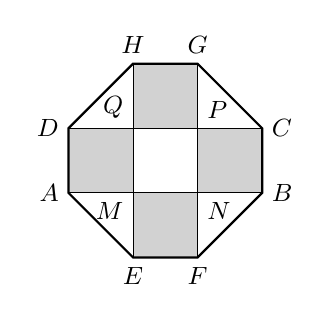
\begin{tikzpicture}[scale=0.82, every node/.style={font=\small}]
  \fill[gray!35] (-1.5,-0.5) rectangle (1.5,0.5);
  \fill[gray!35] (-0.5,-1.5) rectangle (0.5,1.5);
  % 中心正方形 MNPQ 原卷不涂阴影，照原卷留白：
  \fill[white] (-0.5,-0.5) rectangle (0.5,0.5);
  \draw[thick] (-1.5,0.5)--(-0.5,1.5)--(0.5,1.5)--(1.5,0.5)--(1.5,-0.5)--(0.5,-1.5)--(-0.5,-1.5)--(-1.5,-0.5)--cycle;
  \draw (-1.5,-0.5) rectangle (1.5,0.5);
  \draw (-0.5,-1.5) rectangle (0.5,1.5);
  \node[left] at (-1.5,0.5) {$D$};
  \node[left] at (-1.5,-0.5) {$A$};
  \node[right] at (1.5,0.5) {$C$};
  \node[right] at (1.5,-0.5) {$B$};
  \node[above] at (-0.5,1.5) {$H$};
  \node[above] at (0.5,1.5) {$G$};
  \node[below] at (-0.5,-1.5) {$E$};
  \node[below] at (0.5,-1.5) {$F$};
  \node[below left] at (-0.5,-0.5) {$M$};
  \node[below right] at (0.5,-0.5) {$N$};
  \node[above right] at (0.5,0.5) {$P$};
  \node[above left] at (-0.5,0.5) {$Q$};
\end{tikzpicture}
\end{center}

\begin{enumerate}[label=(\arabic*)]
\item 设 $DQ$ 长为 $y$（单位：m），用 $x$ 表示 $y$，并求出 $x$ 的取值范围；
\item $AD$ 取何值时可使总造价最低，并求出最低造价.
\end{enumerate}

\ifanswer
\solbegin
\stepm{(1)}{设 $AD=x\text{m}$（$x>0$），$DQ=y\text{m}$（$y>0$），}
\step{因为十字形区域总面积为 $200\text{m}^2$，所以 $4xy+x^2=200$，}
\step{解得 $y=\dfrac{200-x^2}{4x}=\dfrac{50}{x}-\dfrac{x}{4}$，}
\step{因为 $x>0$，$y>0$，所以 $y=\dfrac{200-x^2}{4x}>0$，解得 $0<x<10\sqrt2$，}
\step{所以 $y=\dfrac{50}{x}-\dfrac{x}{4}$，$0<x<10\sqrt2$；}
\stepm{(2)}{中心正方形 $MNPQ$ 区域，造价为 $2100$ 元$/\text{m}^2$，}
\step{中心正方形 $MNPQ$ 面积为 $S_1=x^2$，造价为 $W_1=2100\times S_1=2100x^2$；}
\step{周围四个矩形区域（图中阴影部分）铺设透水地砖，造价为 $105$ 元$/\text{m}^2$，}
\step{四个矩形的总面积为 $S_2=4xy=4x\left(\dfrac{50}{x}-\dfrac{x}{4}\right)=200-x^2$，}
\step{造价为 $W_2=105\times S_2=105(200-x^2)=21000-105x^2$；}
\step{四个三角形区域种植耐旱固碳植物，助力碳中和，造价为 $40$ 元$/\text{m}^2$，}
\step{四个三角形的总面积为 $S_3=4\times\dfrac12y^2=2\left(\dfrac{50}{x}-\dfrac{x}{4}\right)^2
=\dfrac{5000}{x^2}-50+\dfrac{x^2}{8}$，}
\step{造价为 $W_3=40\times S_3=40\left(\dfrac{5000}{x^2}-50+\dfrac{x^2}{8}\right)
=\dfrac{200000}{x^2}-2000+5x^2$；}
\step{设总造价为 $W$（单位：元），}
\step{则总造价为 $W=W_1+W_2+W_3$}
\step{$=2100x^2+21000-105x^2+\dfrac{200000}{x^2}-2000+5x^2$}
\step{$=2000x^2+\dfrac{200000}{x^2}+19000$，}
\step{又 $2000x^2+\dfrac{200000}{x^2}\geqslant2\sqrt{2000x^2\times\dfrac{200000}{x^2}}=2\times20000=40000$，}
\step{当且仅当 $2000x^2=\dfrac{200000}{x^2}$，即 $x=\sqrt{10}$（在 $x$ 的范围内）时取等号，}
\step{所以 $W=2000x^2+\dfrac{200000}{x^2}+19000\geqslant59000$，当 $x=\sqrt{10}$ 时取等号，}
\step{故当 $AD$ 的长为 $\sqrt{10}$ 时，总造价最低，为 $59000$ 元.}
\solend

\fi

\ansspace[8]

\item 对于实数 $a$、$b$、$c$，若 $|a-c|<|b-c|$，则称 $a$ 比 $b$ 更接近于 $c$. 现已知 $p$、$q$ 都是正有理数.

\begin{enumerate}[label=(\arabic*)]
\item 证明：$\sqrt3$ 必在 $\dfrac pq$ 和 $\dfrac{p+3q}{p+q}$ 之间；
\item 试问 $\dfrac pq$ 和 $\dfrac{p+3q}{p+q}$ 这两个数，哪一个更接近于 $\sqrt3$？说明你的理由；
\item 请你再写出一个有理数，使得它的值比 $\dfrac pq$ 和 $\dfrac{p+3q}{p+q}$ 的值更接近于 $\sqrt3$，并说明你的理由.
\end{enumerate}

\ifanswer
\solbegin
\stepm{(1)}{设 $a=\dfrac pq$（$a$ 为正有理数），则需证 $\sqrt3$ 在 $a$ 和 $\dfrac{a+3}{a+1}$（即 $\dfrac{p+3q}{p+q}$）之间.}
\step{当 $a>\sqrt3$ 时，计算 $a-\dfrac{a+3}{a+1}$ 得 $a-\dfrac{a+3}{a+1}=\dfrac{a(a+1)-(a+3)}{a+1}=\dfrac{a^2-3}{a+1}$，}
\step{$a>\sqrt3$，则 $a^2-3>0$，故 $a>\dfrac{a+3}{a+1}$；}
\step{再计算 $\dfrac{a+3}{a+1}-\sqrt3$ 得 $\dfrac{a+3}{a+1}-\sqrt3=\dfrac{(1-\sqrt3)(a-\sqrt3)}{a+1}$，}
\step{$1-\sqrt3<0$，$a-\sqrt3>0$，$a+1>0$，}
\step{故 $\dfrac{a+3}{a+1}-\sqrt3<0$，即 $\dfrac{a+3}{a+1}<\sqrt3$，从而 $\dfrac{a+3}{a+1}<\sqrt3<a$；}
\step{当 $a<\sqrt3$ 时，同理可得 $a<\dfrac{a+3}{a+1}$ 且 $\dfrac{a+3}{a+1}>\sqrt3$，即 $a<\sqrt3<\dfrac{a+3}{a+1}$，}
\step{综上，$\sqrt3$ 必在 $\dfrac pq$ 和 $\dfrac{p+3q}{p+q}$ 之间；}
\stepm{(2)}{设 $a=\dfrac pq$，$b=\dfrac{p+3q}{p+q}=\dfrac{a+3}{a+1}$，比较 $|a-\sqrt3|$ 与 $|b-\sqrt3|$，}
\step{由（1）得 $(a-\sqrt3)(b-\sqrt3)<0$，}
\step{$\dfrac{|b-\sqrt3|}{|a-\sqrt3|}
=\left|\dfrac{b-\sqrt3}{a-\sqrt3}\right|
=\dfrac{\left|\dfrac{(1-\sqrt3)(a-\sqrt3)}{a+1}\right|}{|a-\sqrt3|}
=\dfrac{\sqrt3-1}{a+1}$，}
\step{$a>0$，$a+1>1$，$\sqrt3-1<1$，故 $\dfrac{\sqrt3-1}{a+1}<1$，即 $|b-\sqrt3|<|a-\sqrt3|$，}
\step{即 $\dfrac{p+3q}{p+q}$ 比 $\dfrac pq$ 更接近于 $\sqrt3$；}
\stepm{(3)}{$\dfrac{2p+3q}{p+2q}$，理由：}
\step{设 $b=\dfrac{p+3q}{p+q}$，新数 $c=\dfrac{b+3}{b+1}=\dfrac{2p+3q}{p+2q}$，}
\step{由（1）得 $(b-\sqrt3)(c-\sqrt3)<0$，}
\step{$c-\sqrt3=\dfrac{b+3}{b+1}-\sqrt3=\dfrac{(1-\sqrt3)(b-\sqrt3)}{b+1}$，}
\step{则 $\dfrac{|c-\sqrt3|}{|b-\sqrt3|}
=\left|\dfrac{c-\sqrt3}{b-\sqrt3}\right|
=\dfrac{\left|\dfrac{(1-\sqrt3)(b-\sqrt3)}{b+1}\right|}{|b-\sqrt3|}
=\dfrac{\sqrt3-1}{b+1}$，}
\step{$b>0$，$b+1>1$，$0<\sqrt3-1<1$，故 $\dfrac{\sqrt3-1}{b+1}<1$，即 $|c-\sqrt3|<|b-\sqrt3|$，}
\step{即 $\dfrac{2p+3q}{p+2q}$ 比 $\dfrac{p+3q}{p+q}$ 更接近于 $\sqrt3$，故 $c$ 更接近 $\sqrt3$.}
\solend

\fi

\ansspace*[10]

\end{enumerate}

\end{document}
"
% 紧凑版：xelatex "\def\iscompact{1}% 高一45_交附闵行_国庆作业2.tex
%   —— 高一上数学“2026-2027 年交附闵行高一上国庆作业 2”（试卷版/答案版）
% 试卷版：xelatex 高一45_交附闵行_国庆作业2.tex
% 答案版：xelatex "\def\isanswer{1}% 高一45_交附闵行_国庆作业2.tex
%   —— 高一上数学“2026-2027 年交附闵行高一上国庆作业 2”（试卷版/答案版）
% 试卷版：xelatex 高一45_交附闵行_国庆作业2.tex
% 答案版：xelatex "\def\isanswer{1}\input{高一45_交附闵行_国庆作业2.tex}"
% 紧凑版：xelatex "\def\iscompact{1}\input{高一45_交附闵行_国庆作业2.tex}"
%
% 原始材料是微信公众号图文（公众号“魔都数学加油站”，作者“破晓”，2026-10-02 17:56 发布，
% 连载“27学年高一45”，原文标题“27学年高一45——2026-2027年上海市交附闵行高一上国庆作业2”，
% https://mp.weixin.qq.com/s/1xdCtzH-3Il0jJrz3saiPA），正文为 10 张 PNG 页。
% 第 01—06、09 页为 4762×6735；第 07、08、10 页为 2560×3620（同一篇各页原图分辨率不一致）。
% 原文本身是一份讲评版：第 3—21 题均照原卷保留题目与题下解析；第 13 题原卷把答案 C 印在括号中。
% 题目、选项、答案与解析均照原卷录入，未改内容；卷面的粉色斜水印及页脚不录入。
%
% 卷首标题：原卷印作“2026-2027 年交附闵行高一上国庆作业 2”（公众号标题里的“上海市”
% 三字卷面标题行没有，本稿照卷面），年份区间按全稿惯例排 en dash，前缀照原卷保留“年”。
%
% 与原卷的排版差异：
%   ① 原卷印有“一、填空题”“二、选择题”“三、解答题”三节标题，本稿照原卷分节，
%      只把标题改排成全稿统一的“大节标题”样式；
%   ② 第 13 题原卷在题干括号内直接印答案 C，本稿按全稿样式将括号留空、答案移入答案版的 \ans{}；
%   ③ 原卷填空横线及选择题答案括号均按全稿样式排版，填空横线统一用 \blankline[4.4em]；
%   ④ 原卷第 20 题配有十字形广场示意图，本稿在源码中用 TikZ 重绘，图中区域、边界及点名照原卷。
%   ⑤ 原卷未印副标题，本稿按本卷实际涉及的知识模块补出“集合与常用逻辑用语、不等式”。
%
% 原卷存疑/错误（均照抄原卷、未改，见对应题目处上方注释）：
%   ① 第 11 题解析原卷印"所以 p=3+9=12，又 12,15∉A，所以 12,15∉B"，与 A∪\overline{B} 的条件
%      及后文 B 的根为 6、9 均一致，无矛盾，本稿照录（早前记录的"∈B／前后矛盾"系本稿误读）；
%   ② 第 15 题题干与解析均按原卷印 ac<0，解析"因为 a<b<c，且 ac<0，所以 a<0，c>0"与题设一致，
%      无矛盾（早前记录的"abc<0／解析冲突"系本稿误读题干所致）；本稿照录原卷答案与解析。
%   ③ 第 20 题原卷各数（造价 2100 元/m^2、W_1=2100x^2、合并式 2000x^2+200000/x^2+19000、
%      末句 59000 元）经复核自洽，无矛盾（早前记录的"W_1=200x^2／末句 5900 元"系本稿误录）；本稿照录。
%   ④ 第 18(2) 题 a=-1 时 A=B=(-1,1)，不满足“B 是 A 的真子集”，故原解析给出的 a≤-1 应为 a<-1；
%   ⑤ 第 19(2) 题原卷用"{c|0<c<1}∩{c|c<-2√3/3 或 c>2√3/3}=∅"论证"不等式①、②中至多有一个恒成立"，
%      论证成立（早前记录的"区间并集留有间隙"系本稿误录解析所致）；本稿照录原卷。
%
\documentclass[a4paper,11pt]{article}
\usepackage{common}

\begin{document}

\examtitlest[3]{2026--2027 年交附闵行高一上国庆作业 2}{集合与常用逻辑用语、不等式}

\bigsec{一、填空题}

\begin{enumerate}
\setcounter{enumi}{2}

\item 满足 $A\cup\{-1,1\}=\{-1,0,1\}$ 的集合 $A$ 共有 \blankline[4.4em] 个.

\ifanswer
\solbegin
\step{集合可能为 $\{0\}$、$\{0,1\}$、$\{0,-1\}$、$\{0,1,-1\}$，共有 $4$ 个.}
\solend

\fi

\item 设 $x\in\R$，则“$x+\dfrac1x>2$”是“$x\neq1$”的 \blankline[4.4em] 条件.

\ifanswer
\solbegin
\step{$x+\dfrac1x>2\Longleftrightarrow x>0$ 且 $x\neq1$，故为充分不必要条件.}
\solend

\fi

\item 已知集合 $A=\{x\mid|x-1|<a\}$，$B=\{-4,3\}$，若 $A\cap B=\varnothing$，则 $a$ 的最大值为 \blankline[4.4em].

\ifanswer
\solbegin
\step{$A=\{x\mid -a<x-1<a\}=\{x\mid1-a<x<1+a\}$，$B=\{-4,3\}$，且 $A\cap B=\varnothing$，}
\step{$A=\varnothing$ 时，$1-a\geqslant1+a$，解得 $a\leqslant0$，满足 $A\cap B=\varnothing$；}
\step{若 $-4\in A$，则 $1-a<-4<1+a$，解得 $a>5$；}
\step{若 $3\in A$，则 $1-a<3<1+a$，解得 $a>2$，}
\step{因为 $A\cap B=\varnothing$，所以 $-4\notin A$ 且 $3\notin A$，所以 $a\leqslant5$ 且 $a\leqslant2$，所以 $a\leqslant2$，}
\step{综上，$a$ 的最大值为 $2$.}
\solend

\fi

\item 设 $x\in\R$，方程 $|x-1|+|2x-1|=|3x-2|$ 的解集为 \blankline[4.4em].

\ifanswer
\solbegin
\step{因为 $|x-1|+|2x-1|\geqslant|(x-1)+(2x-1)|=|3x-2|$，}
\step{当且仅当 $(x-1)(2x-1)\geqslant0$，解得 $x\leqslant\dfrac12$ 或 $x\geqslant1$，}
\step{故方程 $|x-1|+|2x-1|=|3x-2|$ 的解集为 $\left(-\infty,\dfrac12\right]\cup[1,+\infty)$.}
\solend

\fi

\item 已知 $a$、$b\in\R$，且 $3a+2b=1$，则 $8^a+4^b$ 最小值为 \blankline[4.4em].

\ifanswer
\solbegin
% 注：原卷本行与上行均作“$8^a+4^b$ 最小值为”，“最小值”前无“的”，原卷如此，照录未改。
\step{因为 $3a+2b=1$，所以 $8^a+4^b=2^{3a}+2^{2b}\geqslant2\sqrt{2^{3a+2b}}=2\sqrt2$，}
\step{当且仅当 $3a=2b$ 时取等号，故 $8^a+4^b$ 最小值为 $2\sqrt2$.}
\solend

\fi

\item 已知 $a>0$，$b>0$，且 $a+2b+ab=30$，则 $2a+b$ 的最小值为 \blankline[4.4em].

\ifanswer
\solbegin
\step{由 $a+2b+ab=30$，得 $(a+2)(b+1)=32$.}
\step{因为 $a>0$，$b>0$，所以 $a+2>0$，$b+1>0$，}
\step{所以 $2a+b=2(a+2)+(b+1)-5\geqslant2\sqrt{2\times32}-5=11$，}
\step{当且仅当 $2(a+2)=(b+1)$，即 $a=2$，$b=7$ 时取等号，}
\step{所以 $2a+b$ 的最小值为 $11$.}
\solend

\fi

\item 已知 $A=\{x\mid x^2+px+1=0\}$，$M=\{x\mid x>0\}$，若 $A\cap M=\varnothing$，则实数 $p$ 的取值范围为 \blankline[4.4em].

\ifanswer
\solbegin
\step{①当 $A=\varnothing$ 时，$\Delta=p^2-4<0$，所以 $-2<p<2$，此时满足 $A\cap M=\varnothing$；}
\step{②当 $A\neq\varnothing$ 时，$\Delta=p^2-4\geqslant0$，$p\geqslant2$ 或 $p\leqslant-2$，}
\step{因为 $M=\{x\mid x>0\}$，$A\cap M=\varnothing$，由韦达定理得 $\begin{cases}-p\leqslant0\\1>0\end{cases}$，解得 $p\geqslant0$，}
\step{所以 $p\geqslant2$，}
\step{由①②综合得 $p>-2$，故实数 $p$ 的取值范围为 $(-2,+\infty)$.}
\solend

\fi

\item 已知集合 $A=[t,t+1]\cup[t+3,t+6]$，其中 $t>0$. 若存在正数 $\lambda$，使得对任意 $a\in A$，都有 $\dfrac{\lambda}{a}\in A$，则 $t$ 的取值集合为 \blankline[4.4em].

\ifanswer
\solbegin
\step{因为 $0\notin A$，$t>0$，所以 $a\in[t,t+1]\cup[t+3,t+6]$，}
\step{则 $\dfrac1a\in\left[\dfrac1{t+6},\dfrac1{t+3}\right]\cup\left[\dfrac1{t+1},\dfrac1t\right]$，}
\step{又因为 $\lambda>0$，所以 $\dfrac{\lambda}{a}\in\left[\dfrac{\lambda}{t+6},\dfrac{\lambda}{t+3}\right]\cup\left[\dfrac{\lambda}{t+1},\dfrac{\lambda}{t}\right]$，}
\step{因为 $\dfrac{\lambda}{a}\in A$，所以 $\begin{cases}\dfrac{\lambda}{t+6}\geqslant t\\[3pt]\dfrac{\lambda}{t+3}\leqslant t+1\end{cases}$ 且 $\begin{cases}\dfrac{\lambda}{t+1}\geqslant t+3\\[3pt]\dfrac{\lambda}{t}\leqslant t+6\end{cases}$，}
% 注：原卷本行两个不等式组印作“$t(t+6)\leqslant\lambda\leqslant t(t+6)$”与
%     “$(t+1)(t+3)\leqslant\lambda\leqslant(t+1)(t+3)$”（两侧同式），与上行两式推导不合，系原卷笔误；
%     原卷如此，照录未改。
\step{得 $\begin{cases}t(t+6)\leqslant\lambda\leqslant t(t+6)\\[3pt](t+1)(t+3)\leqslant\lambda\leqslant(t+1)(t+3)\end{cases}$，所以 $\lambda=t(t+6)=(t+1)(t+3)$，}
\step{解得 $t=\dfrac32$，取值集合为 $\left\{\dfrac32\right\}$.}
\solend

\fi

\item 已知全集 $U=\{x\mid x=3n,1\leqslant n\leqslant5\ \text{且}\ n\in\N\}$，$A=\{x\mid x^2-px+27=0,p\in\N\}$，
$B=\{x\mid x^2-15x+q=0,q\in\N\}$，且 $A\cup\overline{B}=\{3,9,12,15\}$，则 $p+q$ 的值为 \blankline[4.4em].

\ifanswer
\solbegin
\step{因为全集 $U=\{3,6,9,12,15\}$，$A\cup\overline{B}=\{3,9,12,15\}$，}
\step{所以 $3$、$9$、$12$、$15$ 中可能有两个属于 $A$，}
\step{因为 $A$ 中的方程 $x^2-px+27=0$ 中，两根之积 $x_1x_2=27$，所以 $3$、$9\in A$，}
\step{所以 $p=3+9=12$，又 $12$、$15\notin A$，所以 $12$、$15\notin B$，}
\step{因为 $B$ 中的方程 $x^2-15x+q=0$ 中，两根之和 $x_3+x_4=15$，所以 $6$、$9\in B$，}
\step{则 $q=6\times9=54$，所以 $p+q=66$.}
\solend

\fi

\item 若关于 $x$ 的不等式 $|x-2k|+|x-3k|<4k$ 共有 $2025$ 个整数解，则实数 $k$ 的取值范围为 \blankline[4.4em].

\ifanswer
\solbegin
\step{显然 $k>0$，由 $|x-2k|+|x-3k|<4k$，得 $\dfrac{k}{2}<x<\dfrac{9k}{2}$，}
\step{因为该不等式共有 $2025$ 个整数解，所以 $2024<\dfrac{9k}{2}-\dfrac{k}{2}\leqslant2026$，}
\step{解得 $506<k\leqslant506.5$，}
\step{由 $\dfrac{k}{2}\in(253,253.25]$，得这 $2025$ 个整数解只能为 $254,255,256,\cdots,2278$，}
\step{所以 $2278<\dfrac{9k}{2}\leqslant2279$，解得 $506\dfrac29<k\leqslant506\dfrac49$，结合 $506<k\leqslant506.5$，}
\step{得 $k$ 的取值范围是 $\left(506\dfrac29,506\dfrac49\right]$.}
\solend

\fi

\end{enumerate}

\bigsec{二、选择题}

\begin{enumerate}
\setcounter{enumi}{12}

\item 已知 $a,b\in\R$，且 $ab\neq0$，则下列结论恒成立的是\mbox{（\quad）}

\keepwithprev
A. $a+b\geqslant2\sqrt{ab}$\qquad
B. $\left(\dfrac{a+b}{2}\right)^2>ab$\qquad
C. $\left|\dfrac ab+\dfrac ba\right|\geqslant2$\qquad
D. $a^2+b^2>2ab$

\ans{$C$}

\item 如果 $a^{2025}+b^{2025}=0$，那么一定有\mbox{（\quad）}

\keepwithprev
A. $(|a|+|b|)^{2025}=0$\qquad
B. $(a-b)^{2025}=0$\qquad
C. $(a\cdot b)^{2025}=0$\qquad
D. $(a+b)^{2025}=0$

\ans{$D$}

\ifanswer
\solbegin
\step{由 $a^{2025}+b^{2025}=0$，得 $a^{2025}=-b^{2025}=(-b)^{2025}$，则 $\left(a^{2025}\right)^{\frac{1}{2025}}=\left[(-b)^{2025}\right]^{\frac{1}{2025}}$，}
\step{即 $a=-b$，即 $a+b=0$，故 $(a+b)^{2025}=0$，故 D 符合题意；}
\step{对于 A，若取 $a=1$，$b=-1$，则 $(|a|+|b|)^{2025}=2^{2025}\neq0$，故 A 不合题意；}
\step{对于 B，若取 $a=1$，$b=-1$，则 $(a-b)^{2025}=2^{2025}\neq0$，故 B 不合题意；}
\step{对于 C，若取 $a=1$，$b=-1$，则 $(a\cdot b)^{2025}=(-1)^{2025}=-1\neq0$，故 C 不合题意；}
\step{故选 D.}
\solend

\fi

\item 已知 $a$、$b$、$c$ 满足 $a<b<c$，且 $ac<0$，那么下列各式中一定成立的是\mbox{（\quad）}

\keepwithprev
A. $\dfrac1a>\dfrac1c$\qquad
B. $ab^2<cb^2$\qquad
C. $ac<bc$\qquad
D. $a+c>2b$

\ans{$C$}

\ifanswer
\solbegin
\step{因为 $a<b<c$，且 $ac<0$，所以 $a<0$，$c>0$，}
\step{对于 A，$\dfrac1a<0<\dfrac1c$，故 A 错误；}
\step{对于 B，当 $b=0$ 时，$ab^2=cb^2$，故 B 错误；}
\step{对于 C，$ac<bc$ 可化为 $(a-b)c<0$，因为 $a<b$，所以 $a-b<0$，}
\step{又因为 $c>0$，所以 $(a-b)c<0$，所以 C 正确；}
\step{对于 D，设 $a=-2$，$b=0$，$c=1$，则 $a+c<2b$，故 D 错误.}
\step{故选 C.}
\solend

\fi

\item 对于 $a\in\R$，设集合 $A=\left\{x\mid\dfrac{(x^2-6x+a)(x-1)}{x+a}=0\right\}$，记 $A$ 的所有元素之和为 $S(a)$，
所有元素之积为 $T(a)$，则下列说法中，正确的是\mbox{（\quad）}

\keepwithprev
A. 不存在实数 $a$，使得 $S(a)=6$\qquad
B. 存在实数 $a$，使得 $T(a)=9$

C. 存在无数实数 $a$，使得 $S(a)=7$\qquad
D. 若 $T(a)=3$，则 $a=3$

\ans{$C$}

\ifanswer
\solbegin
\step{要使 $\dfrac{(x^2-6x+a)(x-1)}{x+a}=0$，只需 $(x^2-6x+a)(x-1)=0$ 且 $x+a\neq0$，}
\step{由 $(x^2-6x+a)(x-1)=0$ 得 $x^2-6x+a=0$ 或 $x-1=0$，}
\step{对于一元二次方程 $x^2-6x+a=0$，其判别式 $\Delta=36-4a$，}
\step{当 $\Delta=0$，即 $a=9$ 时，集合 $A=\{1,3\}$，$S(a)=4$，$T(a)=3$；}
\step{当 $\Delta<0$，即 $a>9$ 时，集合 $A=\{1\}$，$S(a)=T(a)=1$；}
\step{当 $\Delta>0$，即 $a<9$ 时，一元二次方程 $x^2-6x+a=0$ 的解为 $x=3\pm\sqrt{9-a}$，}
\step{①当 $a=0$ 时，$x\neq0$，则集合 $A=\{1,6\}$，则 $S(a)=7$，$T(a)=6$，}
\step{②当 $a=-7$ 时，$x\neq7$，则集合 $A=\{-1,1\}$，则 $S(a)=0$，$T(a)=-1$，}
% 注：下一行集合 A 原卷印作 {-1,1}（按 a=-1 代入 x^2-6x-1=0 应得 3±√10，原卷如此，照录未改）。
\step{③当 $a=-1$ 时，$x\neq1$，则集合 $A=\{-1,1\}$，则 $S(a)=6$，$T(a)=-1$，}
\step{④当 $a=5$ 时，$x\neq-5$，则集合 $A=\{1,5\}$，则 $S(a)=6$，$T(a)=5$，}
\step{⑤当 $a\neq5,0,-1,-7$ 时，集合 $A=\{1,3-\sqrt{9-a},3+\sqrt{9-a}\}$，}
\step{则 $S(a)=7$，$T(a)=a$.}
\step{选项 A，当 $a=5$ 时，$S(a)=6$，所以 A 错误；}
\step{选项 B，$T(a)$ 的可能值为 $-1,1,3,5,6,a$（$a<9$），无 $T(a)=9$，所以 B 错误；}
\step{选项 C，当 $a<9$，且 $a\neq5,-1,-7$ 时，$S(a)=7$，有无数个 $a$ 满足，所以 C 正确；}
\step{选项 D，当 $T(a)=3$ 时，有 $a=3$ 和 $a=9$ 满足，所以 D 错误.}
\step{故选 C.}
\solend

\fi

\end{enumerate}

\bigsec{三、解答题}

\begin{enumerate}
\setcounter{enumi}{16}

\item 已知 $a\in\R$，关于 $x$ 的不等式 $|x+1|+|x-1|>a^2-5a+4$.

\begin{enumerate}[label=(\arabic*)]
\item 当 $a=0$ 时，求不等式的解集；
\item 若不等式的解集为 $\R$，求 $a$ 的取值范围.
\end{enumerate}

\ifanswer
\solbegin
\stepm{(1)}{当 $a=0$ 时，不等式为 $|x+1|+|x-1|>4$，}
\step{又 $|x+1|+|x-1|=\begin{cases}2x,&x\geqslant1\\2,&-1<x<1\\-2x,&x\leqslant-1\end{cases}$，}
\step{则 $|x+1|+|x-1|>4$ 的解为 $x>2$ 或 $x<-2$，}
\step{即不等式的解集为 $(-\infty,-2)\cup(2,+\infty)$；}
\stepm{(2)}{不等式 $|x+1|+|x-1|>a^2-5a+4$ 的解集为 $\R$，}
\step{则 $(|x+1|+|x-1|)_{\min}>a^2-5a+4$，}
\step{又 $(|x+1|+|x-1|)_{\min}=2$，当且仅当 $-1\leqslant x\leqslant1$ 时取得，即 $a^2-5a+4<2$，}
\step{即 $a^2-5a+2<0$，即 $\dfrac{5-\sqrt{17}}2<a<\dfrac{5+\sqrt{17}}2$，}
\step{即 $a$ 的取值范围为 $\left(\dfrac{5-\sqrt{17}}2,\dfrac{5+\sqrt{17}}2\right)$.}
\solend

\fi

\ansspace[6]

\item 已知集合 $A=\{x\mid(x-a)(x-a^2)<0\}$，集合 $B=\left\{x\mid\dfrac{2x}{x-1}<1\right\}$，命题 $p:x\in A$，命题 $q:x\in B$.

\begin{enumerate}[label=(\arabic*)]
\item 当实数 $a$ 为何值时，$A=B$；
\item 若 $q$ 是 $p$ 的充分不必要条件，求实数 $a$ 的取值范围.
\end{enumerate}

\ifanswer
\solbegin
\stepm{(1)}{由 $\dfrac{2x}{x-1}<1$ 得 $\dfrac{2x}{x-1}-1=\dfrac{x+1}{x-1}<0$，解得 $-1<x<1$，即 $B=\{x\mid-1<x<1\}$，}
\step{因为 $A=\{x\mid(x-a)(x-a^2)<0\}$，$A=B$，所以 $\begin{cases}a=-1\\a^2=1\end{cases}$，解得 $a=-1$；}
\stepm{(2)}{若 $q$ 是 $p$ 的充分不必要条件，则 $B\subset A$，}
\step{当 $a^2=a$，即 $a=0$ 或 $a=1$ 时，$A=\varnothing$，显然不符合题意；}
\step{当 $a^2>a$，即 $a>1$ 或 $a<0$ 时，$A=(a,a^2)$，则 $\begin{cases}a\leqslant-1\\a^2\geqslant1\\a>1\ \text{或}\ a<0\end{cases}$，}
% 注：a=-1 时 A=(-1,1)=B，不是 B 的真子集；原解析用 B⊂A 但答案含 -1，照录。
\step{前两等号不能同时取得，解得 $a\leqslant-1$；}
\step{当 $a^2<a$，即 $0<a<1$ 时，$A=(a^2,a)$，显然不符合题意，}
\step{故 $a$ 的范围为 $\{a\mid a\leqslant-1\}$.}
\solend

\fi

\ansspace[6]

\item 已知不等式① $x^2+2cx+c>0$，② $x^2+cx+c^2-1>0$，其中 $c$ 是实数.

\begin{enumerate}[label=(\arabic*)]
\item 若 $1$ 是不等式②的一个解，求实数 $c$ 的取值范围；
\item 证明：不等式①、②中至多有一个恒成立.
\end{enumerate}

\ifanswer
\solbegin
\stepm{(1)}{已知不等式① $x^2+2cx+c>0$，② $x^2+cx+c^2-1>0$，}
\step{又 $1$ 是不等式②的一个解，则 $1+c+c^2-1>0$，}
\step{则 $c^2+c>0$，则 $c<-1$ 或 $c>0$，则 $c$ 的取值范围为 $(-\infty,-1)\cup(0,+\infty)$；}
\stepm{(2)}{若不等式①恒成立，则 $\Delta=4c^2-4c<0$，则 $0<c<1$，}
\step{若不等式②恒成立，则 $\Delta=c^2-4(c^2-1)=4-3c^2<0$，}
\step{则 $c<-\dfrac{2\sqrt3}{3}$ 或 $c>\dfrac{2\sqrt3}{3}$，}
\step{又 $\{c\mid 0<c<1\}\cap\left\{c\mid c<-\dfrac{2\sqrt3}{3}\ \text{或}\ c>\dfrac{2\sqrt3}{3}\right\}=\varnothing$，}
\step{则不存在实数 $c$ 使得不等式①、②同时恒成立，}
\step{则不等式①、②中至多有一个恒成立.}
\solend

\fi

\ansspace[6]

\item 为践行“科技强国”战略，某社区计划建造一座融合智慧节能技术的八边形休闲广场，其中两个相同的矩形 $ABCD$ 和 $EFGH$ 构成的十字形区域总面积为 $200\text{m}^2$. 中心正方形 $MNPQ$ 区域将安装国产太阳能光伏板（兼具休憩遮阳功能），造价为 $2100$ 元$/\text{m}^2$；周围四个矩形区域（图中阴影部分）铺设透水地砖，造价为 $105$ 元$/\text{m}^2$；再在四个三角形区域种植耐旱固碳植物，助力碳中和，造价为 $40$ 元$/\text{m}^2$. 设总造价为 $W$（单位：元），$AD=x$（单位：m）.

\begin{center}
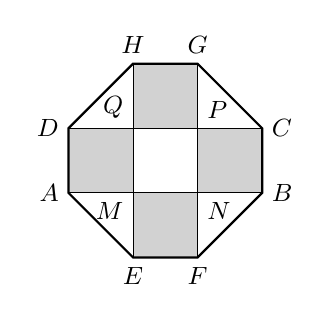
\begin{tikzpicture}[scale=0.82, every node/.style={font=\small}]
  \fill[gray!35] (-1.5,-0.5) rectangle (1.5,0.5);
  \fill[gray!35] (-0.5,-1.5) rectangle (0.5,1.5);
  % 中心正方形 MNPQ 原卷不涂阴影，照原卷留白：
  \fill[white] (-0.5,-0.5) rectangle (0.5,0.5);
  \draw[thick] (-1.5,0.5)--(-0.5,1.5)--(0.5,1.5)--(1.5,0.5)--(1.5,-0.5)--(0.5,-1.5)--(-0.5,-1.5)--(-1.5,-0.5)--cycle;
  \draw (-1.5,-0.5) rectangle (1.5,0.5);
  \draw (-0.5,-1.5) rectangle (0.5,1.5);
  \node[left] at (-1.5,0.5) {$D$};
  \node[left] at (-1.5,-0.5) {$A$};
  \node[right] at (1.5,0.5) {$C$};
  \node[right] at (1.5,-0.5) {$B$};
  \node[above] at (-0.5,1.5) {$H$};
  \node[above] at (0.5,1.5) {$G$};
  \node[below] at (-0.5,-1.5) {$E$};
  \node[below] at (0.5,-1.5) {$F$};
  \node[below left] at (-0.5,-0.5) {$M$};
  \node[below right] at (0.5,-0.5) {$N$};
  \node[above right] at (0.5,0.5) {$P$};
  \node[above left] at (-0.5,0.5) {$Q$};
\end{tikzpicture}
\end{center}

\begin{enumerate}[label=(\arabic*)]
\item 设 $DQ$ 长为 $y$（单位：m），用 $x$ 表示 $y$，并求出 $x$ 的取值范围；
\item $AD$ 取何值时可使总造价最低，并求出最低造价.
\end{enumerate}

\ifanswer
\solbegin
\stepm{(1)}{设 $AD=x\text{m}$（$x>0$），$DQ=y\text{m}$（$y>0$），}
\step{因为十字形区域总面积为 $200\text{m}^2$，所以 $4xy+x^2=200$，}
\step{解得 $y=\dfrac{200-x^2}{4x}=\dfrac{50}{x}-\dfrac{x}{4}$，}
\step{因为 $x>0$，$y>0$，所以 $y=\dfrac{200-x^2}{4x}>0$，解得 $0<x<10\sqrt2$，}
\step{所以 $y=\dfrac{50}{x}-\dfrac{x}{4}$，$0<x<10\sqrt2$；}
\stepm{(2)}{中心正方形 $MNPQ$ 区域，造价为 $2100$ 元$/\text{m}^2$，}
\step{中心正方形 $MNPQ$ 面积为 $S_1=x^2$，造价为 $W_1=2100\times S_1=2100x^2$；}
\step{周围四个矩形区域（图中阴影部分）铺设透水地砖，造价为 $105$ 元$/\text{m}^2$，}
\step{四个矩形的总面积为 $S_2=4xy=4x\left(\dfrac{50}{x}-\dfrac{x}{4}\right)=200-x^2$，}
\step{造价为 $W_2=105\times S_2=105(200-x^2)=21000-105x^2$；}
\step{四个三角形区域种植耐旱固碳植物，助力碳中和，造价为 $40$ 元$/\text{m}^2$，}
\step{四个三角形的总面积为 $S_3=4\times\dfrac12y^2=2\left(\dfrac{50}{x}-\dfrac{x}{4}\right)^2
=\dfrac{5000}{x^2}-50+\dfrac{x^2}{8}$，}
\step{造价为 $W_3=40\times S_3=40\left(\dfrac{5000}{x^2}-50+\dfrac{x^2}{8}\right)
=\dfrac{200000}{x^2}-2000+5x^2$；}
\step{设总造价为 $W$（单位：元），}
\step{则总造价为 $W=W_1+W_2+W_3$}
\step{$=2100x^2+21000-105x^2+\dfrac{200000}{x^2}-2000+5x^2$}
\step{$=2000x^2+\dfrac{200000}{x^2}+19000$，}
\step{又 $2000x^2+\dfrac{200000}{x^2}\geqslant2\sqrt{2000x^2\times\dfrac{200000}{x^2}}=2\times20000=40000$，}
\step{当且仅当 $2000x^2=\dfrac{200000}{x^2}$，即 $x=\sqrt{10}$（在 $x$ 的范围内）时取等号，}
\step{所以 $W=2000x^2+\dfrac{200000}{x^2}+19000\geqslant59000$，当 $x=\sqrt{10}$ 时取等号，}
\step{故当 $AD$ 的长为 $\sqrt{10}$ 时，总造价最低，为 $59000$ 元.}
\solend

\fi

\ansspace[8]

\item 对于实数 $a$、$b$、$c$，若 $|a-c|<|b-c|$，则称 $a$ 比 $b$ 更接近于 $c$. 现已知 $p$、$q$ 都是正有理数.

\begin{enumerate}[label=(\arabic*)]
\item 证明：$\sqrt3$ 必在 $\dfrac pq$ 和 $\dfrac{p+3q}{p+q}$ 之间；
\item 试问 $\dfrac pq$ 和 $\dfrac{p+3q}{p+q}$ 这两个数，哪一个更接近于 $\sqrt3$？说明你的理由；
\item 请你再写出一个有理数，使得它的值比 $\dfrac pq$ 和 $\dfrac{p+3q}{p+q}$ 的值更接近于 $\sqrt3$，并说明你的理由.
\end{enumerate}

\ifanswer
\solbegin
\stepm{(1)}{设 $a=\dfrac pq$（$a$ 为正有理数），则需证 $\sqrt3$ 在 $a$ 和 $\dfrac{a+3}{a+1}$（即 $\dfrac{p+3q}{p+q}$）之间.}
\step{当 $a>\sqrt3$ 时，计算 $a-\dfrac{a+3}{a+1}$ 得 $a-\dfrac{a+3}{a+1}=\dfrac{a(a+1)-(a+3)}{a+1}=\dfrac{a^2-3}{a+1}$，}
\step{$a>\sqrt3$，则 $a^2-3>0$，故 $a>\dfrac{a+3}{a+1}$；}
\step{再计算 $\dfrac{a+3}{a+1}-\sqrt3$ 得 $\dfrac{a+3}{a+1}-\sqrt3=\dfrac{(1-\sqrt3)(a-\sqrt3)}{a+1}$，}
\step{$1-\sqrt3<0$，$a-\sqrt3>0$，$a+1>0$，}
\step{故 $\dfrac{a+3}{a+1}-\sqrt3<0$，即 $\dfrac{a+3}{a+1}<\sqrt3$，从而 $\dfrac{a+3}{a+1}<\sqrt3<a$；}
\step{当 $a<\sqrt3$ 时，同理可得 $a<\dfrac{a+3}{a+1}$ 且 $\dfrac{a+3}{a+1}>\sqrt3$，即 $a<\sqrt3<\dfrac{a+3}{a+1}$，}
\step{综上，$\sqrt3$ 必在 $\dfrac pq$ 和 $\dfrac{p+3q}{p+q}$ 之间；}
\stepm{(2)}{设 $a=\dfrac pq$，$b=\dfrac{p+3q}{p+q}=\dfrac{a+3}{a+1}$，比较 $|a-\sqrt3|$ 与 $|b-\sqrt3|$，}
\step{由（1）得 $(a-\sqrt3)(b-\sqrt3)<0$，}
\step{$\dfrac{|b-\sqrt3|}{|a-\sqrt3|}
=\left|\dfrac{b-\sqrt3}{a-\sqrt3}\right|
=\dfrac{\left|\dfrac{(1-\sqrt3)(a-\sqrt3)}{a+1}\right|}{|a-\sqrt3|}
=\dfrac{\sqrt3-1}{a+1}$，}
\step{$a>0$，$a+1>1$，$\sqrt3-1<1$，故 $\dfrac{\sqrt3-1}{a+1}<1$，即 $|b-\sqrt3|<|a-\sqrt3|$，}
\step{即 $\dfrac{p+3q}{p+q}$ 比 $\dfrac pq$ 更接近于 $\sqrt3$；}
\stepm{(3)}{$\dfrac{2p+3q}{p+2q}$，理由：}
\step{设 $b=\dfrac{p+3q}{p+q}$，新数 $c=\dfrac{b+3}{b+1}=\dfrac{2p+3q}{p+2q}$，}
\step{由（1）得 $(b-\sqrt3)(c-\sqrt3)<0$，}
\step{$c-\sqrt3=\dfrac{b+3}{b+1}-\sqrt3=\dfrac{(1-\sqrt3)(b-\sqrt3)}{b+1}$，}
\step{则 $\dfrac{|c-\sqrt3|}{|b-\sqrt3|}
=\left|\dfrac{c-\sqrt3}{b-\sqrt3}\right|
=\dfrac{\left|\dfrac{(1-\sqrt3)(b-\sqrt3)}{b+1}\right|}{|b-\sqrt3|}
=\dfrac{\sqrt3-1}{b+1}$，}
\step{$b>0$，$b+1>1$，$0<\sqrt3-1<1$，故 $\dfrac{\sqrt3-1}{b+1}<1$，即 $|c-\sqrt3|<|b-\sqrt3|$，}
\step{即 $\dfrac{2p+3q}{p+2q}$ 比 $\dfrac{p+3q}{p+q}$ 更接近于 $\sqrt3$，故 $c$ 更接近 $\sqrt3$.}
\solend

\fi

\ansspace*[10]

\end{enumerate}

\end{document}
"
% 紧凑版：xelatex "\def\iscompact{1}% 高一45_交附闵行_国庆作业2.tex
%   —— 高一上数学“2026-2027 年交附闵行高一上国庆作业 2”（试卷版/答案版）
% 试卷版：xelatex 高一45_交附闵行_国庆作业2.tex
% 答案版：xelatex "\def\isanswer{1}\input{高一45_交附闵行_国庆作业2.tex}"
% 紧凑版：xelatex "\def\iscompact{1}\input{高一45_交附闵行_国庆作业2.tex}"
%
% 原始材料是微信公众号图文（公众号“魔都数学加油站”，作者“破晓”，2026-10-02 17:56 发布，
% 连载“27学年高一45”，原文标题“27学年高一45——2026-2027年上海市交附闵行高一上国庆作业2”，
% https://mp.weixin.qq.com/s/1xdCtzH-3Il0jJrz3saiPA），正文为 10 张 PNG 页。
% 第 01—06、09 页为 4762×6735；第 07、08、10 页为 2560×3620（同一篇各页原图分辨率不一致）。
% 原文本身是一份讲评版：第 3—21 题均照原卷保留题目与题下解析；第 13 题原卷把答案 C 印在括号中。
% 题目、选项、答案与解析均照原卷录入，未改内容；卷面的粉色斜水印及页脚不录入。
%
% 卷首标题：原卷印作“2026-2027 年交附闵行高一上国庆作业 2”（公众号标题里的“上海市”
% 三字卷面标题行没有，本稿照卷面），年份区间按全稿惯例排 en dash，前缀照原卷保留“年”。
%
% 与原卷的排版差异：
%   ① 原卷印有“一、填空题”“二、选择题”“三、解答题”三节标题，本稿照原卷分节，
%      只把标题改排成全稿统一的“大节标题”样式；
%   ② 第 13 题原卷在题干括号内直接印答案 C，本稿按全稿样式将括号留空、答案移入答案版的 \ans{}；
%   ③ 原卷填空横线及选择题答案括号均按全稿样式排版，填空横线统一用 \blankline[4.4em]；
%   ④ 原卷第 20 题配有十字形广场示意图，本稿在源码中用 TikZ 重绘，图中区域、边界及点名照原卷。
%   ⑤ 原卷未印副标题，本稿按本卷实际涉及的知识模块补出“集合与常用逻辑用语、不等式”。
%
% 原卷存疑/错误（均照抄原卷、未改，见对应题目处上方注释）：
%   ① 第 11 题解析原卷印"所以 p=3+9=12，又 12,15∉A，所以 12,15∉B"，与 A∪\overline{B} 的条件
%      及后文 B 的根为 6、9 均一致，无矛盾，本稿照录（早前记录的"∈B／前后矛盾"系本稿误读）；
%   ② 第 15 题题干与解析均按原卷印 ac<0，解析"因为 a<b<c，且 ac<0，所以 a<0，c>0"与题设一致，
%      无矛盾（早前记录的"abc<0／解析冲突"系本稿误读题干所致）；本稿照录原卷答案与解析。
%   ③ 第 20 题原卷各数（造价 2100 元/m^2、W_1=2100x^2、合并式 2000x^2+200000/x^2+19000、
%      末句 59000 元）经复核自洽，无矛盾（早前记录的"W_1=200x^2／末句 5900 元"系本稿误录）；本稿照录。
%   ④ 第 18(2) 题 a=-1 时 A=B=(-1,1)，不满足“B 是 A 的真子集”，故原解析给出的 a≤-1 应为 a<-1；
%   ⑤ 第 19(2) 题原卷用"{c|0<c<1}∩{c|c<-2√3/3 或 c>2√3/3}=∅"论证"不等式①、②中至多有一个恒成立"，
%      论证成立（早前记录的"区间并集留有间隙"系本稿误录解析所致）；本稿照录原卷。
%
\documentclass[a4paper,11pt]{article}
\usepackage{common}

\begin{document}

\examtitlest[3]{2026--2027 年交附闵行高一上国庆作业 2}{集合与常用逻辑用语、不等式}

\bigsec{一、填空题}

\begin{enumerate}
\setcounter{enumi}{2}

\item 满足 $A\cup\{-1,1\}=\{-1,0,1\}$ 的集合 $A$ 共有 \blankline[4.4em] 个.

\ifanswer
\solbegin
\step{集合可能为 $\{0\}$、$\{0,1\}$、$\{0,-1\}$、$\{0,1,-1\}$，共有 $4$ 个.}
\solend

\fi

\item 设 $x\in\R$，则“$x+\dfrac1x>2$”是“$x\neq1$”的 \blankline[4.4em] 条件.

\ifanswer
\solbegin
\step{$x+\dfrac1x>2\Longleftrightarrow x>0$ 且 $x\neq1$，故为充分不必要条件.}
\solend

\fi

\item 已知集合 $A=\{x\mid|x-1|<a\}$，$B=\{-4,3\}$，若 $A\cap B=\varnothing$，则 $a$ 的最大值为 \blankline[4.4em].

\ifanswer
\solbegin
\step{$A=\{x\mid -a<x-1<a\}=\{x\mid1-a<x<1+a\}$，$B=\{-4,3\}$，且 $A\cap B=\varnothing$，}
\step{$A=\varnothing$ 时，$1-a\geqslant1+a$，解得 $a\leqslant0$，满足 $A\cap B=\varnothing$；}
\step{若 $-4\in A$，则 $1-a<-4<1+a$，解得 $a>5$；}
\step{若 $3\in A$，则 $1-a<3<1+a$，解得 $a>2$，}
\step{因为 $A\cap B=\varnothing$，所以 $-4\notin A$ 且 $3\notin A$，所以 $a\leqslant5$ 且 $a\leqslant2$，所以 $a\leqslant2$，}
\step{综上，$a$ 的最大值为 $2$.}
\solend

\fi

\item 设 $x\in\R$，方程 $|x-1|+|2x-1|=|3x-2|$ 的解集为 \blankline[4.4em].

\ifanswer
\solbegin
\step{因为 $|x-1|+|2x-1|\geqslant|(x-1)+(2x-1)|=|3x-2|$，}
\step{当且仅当 $(x-1)(2x-1)\geqslant0$，解得 $x\leqslant\dfrac12$ 或 $x\geqslant1$，}
\step{故方程 $|x-1|+|2x-1|=|3x-2|$ 的解集为 $\left(-\infty,\dfrac12\right]\cup[1,+\infty)$.}
\solend

\fi

\item 已知 $a$、$b\in\R$，且 $3a+2b=1$，则 $8^a+4^b$ 最小值为 \blankline[4.4em].

\ifanswer
\solbegin
% 注：原卷本行与上行均作“$8^a+4^b$ 最小值为”，“最小值”前无“的”，原卷如此，照录未改。
\step{因为 $3a+2b=1$，所以 $8^a+4^b=2^{3a}+2^{2b}\geqslant2\sqrt{2^{3a+2b}}=2\sqrt2$，}
\step{当且仅当 $3a=2b$ 时取等号，故 $8^a+4^b$ 最小值为 $2\sqrt2$.}
\solend

\fi

\item 已知 $a>0$，$b>0$，且 $a+2b+ab=30$，则 $2a+b$ 的最小值为 \blankline[4.4em].

\ifanswer
\solbegin
\step{由 $a+2b+ab=30$，得 $(a+2)(b+1)=32$.}
\step{因为 $a>0$，$b>0$，所以 $a+2>0$，$b+1>0$，}
\step{所以 $2a+b=2(a+2)+(b+1)-5\geqslant2\sqrt{2\times32}-5=11$，}
\step{当且仅当 $2(a+2)=(b+1)$，即 $a=2$，$b=7$ 时取等号，}
\step{所以 $2a+b$ 的最小值为 $11$.}
\solend

\fi

\item 已知 $A=\{x\mid x^2+px+1=0\}$，$M=\{x\mid x>0\}$，若 $A\cap M=\varnothing$，则实数 $p$ 的取值范围为 \blankline[4.4em].

\ifanswer
\solbegin
\step{①当 $A=\varnothing$ 时，$\Delta=p^2-4<0$，所以 $-2<p<2$，此时满足 $A\cap M=\varnothing$；}
\step{②当 $A\neq\varnothing$ 时，$\Delta=p^2-4\geqslant0$，$p\geqslant2$ 或 $p\leqslant-2$，}
\step{因为 $M=\{x\mid x>0\}$，$A\cap M=\varnothing$，由韦达定理得 $\begin{cases}-p\leqslant0\\1>0\end{cases}$，解得 $p\geqslant0$，}
\step{所以 $p\geqslant2$，}
\step{由①②综合得 $p>-2$，故实数 $p$ 的取值范围为 $(-2,+\infty)$.}
\solend

\fi

\item 已知集合 $A=[t,t+1]\cup[t+3,t+6]$，其中 $t>0$. 若存在正数 $\lambda$，使得对任意 $a\in A$，都有 $\dfrac{\lambda}{a}\in A$，则 $t$ 的取值集合为 \blankline[4.4em].

\ifanswer
\solbegin
\step{因为 $0\notin A$，$t>0$，所以 $a\in[t,t+1]\cup[t+3,t+6]$，}
\step{则 $\dfrac1a\in\left[\dfrac1{t+6},\dfrac1{t+3}\right]\cup\left[\dfrac1{t+1},\dfrac1t\right]$，}
\step{又因为 $\lambda>0$，所以 $\dfrac{\lambda}{a}\in\left[\dfrac{\lambda}{t+6},\dfrac{\lambda}{t+3}\right]\cup\left[\dfrac{\lambda}{t+1},\dfrac{\lambda}{t}\right]$，}
\step{因为 $\dfrac{\lambda}{a}\in A$，所以 $\begin{cases}\dfrac{\lambda}{t+6}\geqslant t\\[3pt]\dfrac{\lambda}{t+3}\leqslant t+1\end{cases}$ 且 $\begin{cases}\dfrac{\lambda}{t+1}\geqslant t+3\\[3pt]\dfrac{\lambda}{t}\leqslant t+6\end{cases}$，}
% 注：原卷本行两个不等式组印作“$t(t+6)\leqslant\lambda\leqslant t(t+6)$”与
%     “$(t+1)(t+3)\leqslant\lambda\leqslant(t+1)(t+3)$”（两侧同式），与上行两式推导不合，系原卷笔误；
%     原卷如此，照录未改。
\step{得 $\begin{cases}t(t+6)\leqslant\lambda\leqslant t(t+6)\\[3pt](t+1)(t+3)\leqslant\lambda\leqslant(t+1)(t+3)\end{cases}$，所以 $\lambda=t(t+6)=(t+1)(t+3)$，}
\step{解得 $t=\dfrac32$，取值集合为 $\left\{\dfrac32\right\}$.}
\solend

\fi

\item 已知全集 $U=\{x\mid x=3n,1\leqslant n\leqslant5\ \text{且}\ n\in\N\}$，$A=\{x\mid x^2-px+27=0,p\in\N\}$，
$B=\{x\mid x^2-15x+q=0,q\in\N\}$，且 $A\cup\overline{B}=\{3,9,12,15\}$，则 $p+q$ 的值为 \blankline[4.4em].

\ifanswer
\solbegin
\step{因为全集 $U=\{3,6,9,12,15\}$，$A\cup\overline{B}=\{3,9,12,15\}$，}
\step{所以 $3$、$9$、$12$、$15$ 中可能有两个属于 $A$，}
\step{因为 $A$ 中的方程 $x^2-px+27=0$ 中，两根之积 $x_1x_2=27$，所以 $3$、$9\in A$，}
\step{所以 $p=3+9=12$，又 $12$、$15\notin A$，所以 $12$、$15\notin B$，}
\step{因为 $B$ 中的方程 $x^2-15x+q=0$ 中，两根之和 $x_3+x_4=15$，所以 $6$、$9\in B$，}
\step{则 $q=6\times9=54$，所以 $p+q=66$.}
\solend

\fi

\item 若关于 $x$ 的不等式 $|x-2k|+|x-3k|<4k$ 共有 $2025$ 个整数解，则实数 $k$ 的取值范围为 \blankline[4.4em].

\ifanswer
\solbegin
\step{显然 $k>0$，由 $|x-2k|+|x-3k|<4k$，得 $\dfrac{k}{2}<x<\dfrac{9k}{2}$，}
\step{因为该不等式共有 $2025$ 个整数解，所以 $2024<\dfrac{9k}{2}-\dfrac{k}{2}\leqslant2026$，}
\step{解得 $506<k\leqslant506.5$，}
\step{由 $\dfrac{k}{2}\in(253,253.25]$，得这 $2025$ 个整数解只能为 $254,255,256,\cdots,2278$，}
\step{所以 $2278<\dfrac{9k}{2}\leqslant2279$，解得 $506\dfrac29<k\leqslant506\dfrac49$，结合 $506<k\leqslant506.5$，}
\step{得 $k$ 的取值范围是 $\left(506\dfrac29,506\dfrac49\right]$.}
\solend

\fi

\end{enumerate}

\bigsec{二、选择题}

\begin{enumerate}
\setcounter{enumi}{12}

\item 已知 $a,b\in\R$，且 $ab\neq0$，则下列结论恒成立的是\mbox{（\quad）}

\keepwithprev
A. $a+b\geqslant2\sqrt{ab}$\qquad
B. $\left(\dfrac{a+b}{2}\right)^2>ab$\qquad
C. $\left|\dfrac ab+\dfrac ba\right|\geqslant2$\qquad
D. $a^2+b^2>2ab$

\ans{$C$}

\item 如果 $a^{2025}+b^{2025}=0$，那么一定有\mbox{（\quad）}

\keepwithprev
A. $(|a|+|b|)^{2025}=0$\qquad
B. $(a-b)^{2025}=0$\qquad
C. $(a\cdot b)^{2025}=0$\qquad
D. $(a+b)^{2025}=0$

\ans{$D$}

\ifanswer
\solbegin
\step{由 $a^{2025}+b^{2025}=0$，得 $a^{2025}=-b^{2025}=(-b)^{2025}$，则 $\left(a^{2025}\right)^{\frac{1}{2025}}=\left[(-b)^{2025}\right]^{\frac{1}{2025}}$，}
\step{即 $a=-b$，即 $a+b=0$，故 $(a+b)^{2025}=0$，故 D 符合题意；}
\step{对于 A，若取 $a=1$，$b=-1$，则 $(|a|+|b|)^{2025}=2^{2025}\neq0$，故 A 不合题意；}
\step{对于 B，若取 $a=1$，$b=-1$，则 $(a-b)^{2025}=2^{2025}\neq0$，故 B 不合题意；}
\step{对于 C，若取 $a=1$，$b=-1$，则 $(a\cdot b)^{2025}=(-1)^{2025}=-1\neq0$，故 C 不合题意；}
\step{故选 D.}
\solend

\fi

\item 已知 $a$、$b$、$c$ 满足 $a<b<c$，且 $ac<0$，那么下列各式中一定成立的是\mbox{（\quad）}

\keepwithprev
A. $\dfrac1a>\dfrac1c$\qquad
B. $ab^2<cb^2$\qquad
C. $ac<bc$\qquad
D. $a+c>2b$

\ans{$C$}

\ifanswer
\solbegin
\step{因为 $a<b<c$，且 $ac<0$，所以 $a<0$，$c>0$，}
\step{对于 A，$\dfrac1a<0<\dfrac1c$，故 A 错误；}
\step{对于 B，当 $b=0$ 时，$ab^2=cb^2$，故 B 错误；}
\step{对于 C，$ac<bc$ 可化为 $(a-b)c<0$，因为 $a<b$，所以 $a-b<0$，}
\step{又因为 $c>0$，所以 $(a-b)c<0$，所以 C 正确；}
\step{对于 D，设 $a=-2$，$b=0$，$c=1$，则 $a+c<2b$，故 D 错误.}
\step{故选 C.}
\solend

\fi

\item 对于 $a\in\R$，设集合 $A=\left\{x\mid\dfrac{(x^2-6x+a)(x-1)}{x+a}=0\right\}$，记 $A$ 的所有元素之和为 $S(a)$，
所有元素之积为 $T(a)$，则下列说法中，正确的是\mbox{（\quad）}

\keepwithprev
A. 不存在实数 $a$，使得 $S(a)=6$\qquad
B. 存在实数 $a$，使得 $T(a)=9$

C. 存在无数实数 $a$，使得 $S(a)=7$\qquad
D. 若 $T(a)=3$，则 $a=3$

\ans{$C$}

\ifanswer
\solbegin
\step{要使 $\dfrac{(x^2-6x+a)(x-1)}{x+a}=0$，只需 $(x^2-6x+a)(x-1)=0$ 且 $x+a\neq0$，}
\step{由 $(x^2-6x+a)(x-1)=0$ 得 $x^2-6x+a=0$ 或 $x-1=0$，}
\step{对于一元二次方程 $x^2-6x+a=0$，其判别式 $\Delta=36-4a$，}
\step{当 $\Delta=0$，即 $a=9$ 时，集合 $A=\{1,3\}$，$S(a)=4$，$T(a)=3$；}
\step{当 $\Delta<0$，即 $a>9$ 时，集合 $A=\{1\}$，$S(a)=T(a)=1$；}
\step{当 $\Delta>0$，即 $a<9$ 时，一元二次方程 $x^2-6x+a=0$ 的解为 $x=3\pm\sqrt{9-a}$，}
\step{①当 $a=0$ 时，$x\neq0$，则集合 $A=\{1,6\}$，则 $S(a)=7$，$T(a)=6$，}
\step{②当 $a=-7$ 时，$x\neq7$，则集合 $A=\{-1,1\}$，则 $S(a)=0$，$T(a)=-1$，}
% 注：下一行集合 A 原卷印作 {-1,1}（按 a=-1 代入 x^2-6x-1=0 应得 3±√10，原卷如此，照录未改）。
\step{③当 $a=-1$ 时，$x\neq1$，则集合 $A=\{-1,1\}$，则 $S(a)=6$，$T(a)=-1$，}
\step{④当 $a=5$ 时，$x\neq-5$，则集合 $A=\{1,5\}$，则 $S(a)=6$，$T(a)=5$，}
\step{⑤当 $a\neq5,0,-1,-7$ 时，集合 $A=\{1,3-\sqrt{9-a},3+\sqrt{9-a}\}$，}
\step{则 $S(a)=7$，$T(a)=a$.}
\step{选项 A，当 $a=5$ 时，$S(a)=6$，所以 A 错误；}
\step{选项 B，$T(a)$ 的可能值为 $-1,1,3,5,6,a$（$a<9$），无 $T(a)=9$，所以 B 错误；}
\step{选项 C，当 $a<9$，且 $a\neq5,-1,-7$ 时，$S(a)=7$，有无数个 $a$ 满足，所以 C 正确；}
\step{选项 D，当 $T(a)=3$ 时，有 $a=3$ 和 $a=9$ 满足，所以 D 错误.}
\step{故选 C.}
\solend

\fi

\end{enumerate}

\bigsec{三、解答题}

\begin{enumerate}
\setcounter{enumi}{16}

\item 已知 $a\in\R$，关于 $x$ 的不等式 $|x+1|+|x-1|>a^2-5a+4$.

\begin{enumerate}[label=(\arabic*)]
\item 当 $a=0$ 时，求不等式的解集；
\item 若不等式的解集为 $\R$，求 $a$ 的取值范围.
\end{enumerate}

\ifanswer
\solbegin
\stepm{(1)}{当 $a=0$ 时，不等式为 $|x+1|+|x-1|>4$，}
\step{又 $|x+1|+|x-1|=\begin{cases}2x,&x\geqslant1\\2,&-1<x<1\\-2x,&x\leqslant-1\end{cases}$，}
\step{则 $|x+1|+|x-1|>4$ 的解为 $x>2$ 或 $x<-2$，}
\step{即不等式的解集为 $(-\infty,-2)\cup(2,+\infty)$；}
\stepm{(2)}{不等式 $|x+1|+|x-1|>a^2-5a+4$ 的解集为 $\R$，}
\step{则 $(|x+1|+|x-1|)_{\min}>a^2-5a+4$，}
\step{又 $(|x+1|+|x-1|)_{\min}=2$，当且仅当 $-1\leqslant x\leqslant1$ 时取得，即 $a^2-5a+4<2$，}
\step{即 $a^2-5a+2<0$，即 $\dfrac{5-\sqrt{17}}2<a<\dfrac{5+\sqrt{17}}2$，}
\step{即 $a$ 的取值范围为 $\left(\dfrac{5-\sqrt{17}}2,\dfrac{5+\sqrt{17}}2\right)$.}
\solend

\fi

\ansspace[6]

\item 已知集合 $A=\{x\mid(x-a)(x-a^2)<0\}$，集合 $B=\left\{x\mid\dfrac{2x}{x-1}<1\right\}$，命题 $p:x\in A$，命题 $q:x\in B$.

\begin{enumerate}[label=(\arabic*)]
\item 当实数 $a$ 为何值时，$A=B$；
\item 若 $q$ 是 $p$ 的充分不必要条件，求实数 $a$ 的取值范围.
\end{enumerate}

\ifanswer
\solbegin
\stepm{(1)}{由 $\dfrac{2x}{x-1}<1$ 得 $\dfrac{2x}{x-1}-1=\dfrac{x+1}{x-1}<0$，解得 $-1<x<1$，即 $B=\{x\mid-1<x<1\}$，}
\step{因为 $A=\{x\mid(x-a)(x-a^2)<0\}$，$A=B$，所以 $\begin{cases}a=-1\\a^2=1\end{cases}$，解得 $a=-1$；}
\stepm{(2)}{若 $q$ 是 $p$ 的充分不必要条件，则 $B\subset A$，}
\step{当 $a^2=a$，即 $a=0$ 或 $a=1$ 时，$A=\varnothing$，显然不符合题意；}
\step{当 $a^2>a$，即 $a>1$ 或 $a<0$ 时，$A=(a,a^2)$，则 $\begin{cases}a\leqslant-1\\a^2\geqslant1\\a>1\ \text{或}\ a<0\end{cases}$，}
% 注：a=-1 时 A=(-1,1)=B，不是 B 的真子集；原解析用 B⊂A 但答案含 -1，照录。
\step{前两等号不能同时取得，解得 $a\leqslant-1$；}
\step{当 $a^2<a$，即 $0<a<1$ 时，$A=(a^2,a)$，显然不符合题意，}
\step{故 $a$ 的范围为 $\{a\mid a\leqslant-1\}$.}
\solend

\fi

\ansspace[6]

\item 已知不等式① $x^2+2cx+c>0$，② $x^2+cx+c^2-1>0$，其中 $c$ 是实数.

\begin{enumerate}[label=(\arabic*)]
\item 若 $1$ 是不等式②的一个解，求实数 $c$ 的取值范围；
\item 证明：不等式①、②中至多有一个恒成立.
\end{enumerate}

\ifanswer
\solbegin
\stepm{(1)}{已知不等式① $x^2+2cx+c>0$，② $x^2+cx+c^2-1>0$，}
\step{又 $1$ 是不等式②的一个解，则 $1+c+c^2-1>0$，}
\step{则 $c^2+c>0$，则 $c<-1$ 或 $c>0$，则 $c$ 的取值范围为 $(-\infty,-1)\cup(0,+\infty)$；}
\stepm{(2)}{若不等式①恒成立，则 $\Delta=4c^2-4c<0$，则 $0<c<1$，}
\step{若不等式②恒成立，则 $\Delta=c^2-4(c^2-1)=4-3c^2<0$，}
\step{则 $c<-\dfrac{2\sqrt3}{3}$ 或 $c>\dfrac{2\sqrt3}{3}$，}
\step{又 $\{c\mid 0<c<1\}\cap\left\{c\mid c<-\dfrac{2\sqrt3}{3}\ \text{或}\ c>\dfrac{2\sqrt3}{3}\right\}=\varnothing$，}
\step{则不存在实数 $c$ 使得不等式①、②同时恒成立，}
\step{则不等式①、②中至多有一个恒成立.}
\solend

\fi

\ansspace[6]

\item 为践行“科技强国”战略，某社区计划建造一座融合智慧节能技术的八边形休闲广场，其中两个相同的矩形 $ABCD$ 和 $EFGH$ 构成的十字形区域总面积为 $200\text{m}^2$. 中心正方形 $MNPQ$ 区域将安装国产太阳能光伏板（兼具休憩遮阳功能），造价为 $2100$ 元$/\text{m}^2$；周围四个矩形区域（图中阴影部分）铺设透水地砖，造价为 $105$ 元$/\text{m}^2$；再在四个三角形区域种植耐旱固碳植物，助力碳中和，造价为 $40$ 元$/\text{m}^2$. 设总造价为 $W$（单位：元），$AD=x$（单位：m）.

\begin{center}
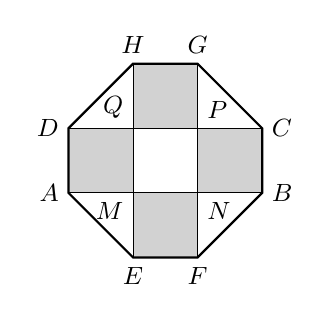
\begin{tikzpicture}[scale=0.82, every node/.style={font=\small}]
  \fill[gray!35] (-1.5,-0.5) rectangle (1.5,0.5);
  \fill[gray!35] (-0.5,-1.5) rectangle (0.5,1.5);
  % 中心正方形 MNPQ 原卷不涂阴影，照原卷留白：
  \fill[white] (-0.5,-0.5) rectangle (0.5,0.5);
  \draw[thick] (-1.5,0.5)--(-0.5,1.5)--(0.5,1.5)--(1.5,0.5)--(1.5,-0.5)--(0.5,-1.5)--(-0.5,-1.5)--(-1.5,-0.5)--cycle;
  \draw (-1.5,-0.5) rectangle (1.5,0.5);
  \draw (-0.5,-1.5) rectangle (0.5,1.5);
  \node[left] at (-1.5,0.5) {$D$};
  \node[left] at (-1.5,-0.5) {$A$};
  \node[right] at (1.5,0.5) {$C$};
  \node[right] at (1.5,-0.5) {$B$};
  \node[above] at (-0.5,1.5) {$H$};
  \node[above] at (0.5,1.5) {$G$};
  \node[below] at (-0.5,-1.5) {$E$};
  \node[below] at (0.5,-1.5) {$F$};
  \node[below left] at (-0.5,-0.5) {$M$};
  \node[below right] at (0.5,-0.5) {$N$};
  \node[above right] at (0.5,0.5) {$P$};
  \node[above left] at (-0.5,0.5) {$Q$};
\end{tikzpicture}
\end{center}

\begin{enumerate}[label=(\arabic*)]
\item 设 $DQ$ 长为 $y$（单位：m），用 $x$ 表示 $y$，并求出 $x$ 的取值范围；
\item $AD$ 取何值时可使总造价最低，并求出最低造价.
\end{enumerate}

\ifanswer
\solbegin
\stepm{(1)}{设 $AD=x\text{m}$（$x>0$），$DQ=y\text{m}$（$y>0$），}
\step{因为十字形区域总面积为 $200\text{m}^2$，所以 $4xy+x^2=200$，}
\step{解得 $y=\dfrac{200-x^2}{4x}=\dfrac{50}{x}-\dfrac{x}{4}$，}
\step{因为 $x>0$，$y>0$，所以 $y=\dfrac{200-x^2}{4x}>0$，解得 $0<x<10\sqrt2$，}
\step{所以 $y=\dfrac{50}{x}-\dfrac{x}{4}$，$0<x<10\sqrt2$；}
\stepm{(2)}{中心正方形 $MNPQ$ 区域，造价为 $2100$ 元$/\text{m}^2$，}
\step{中心正方形 $MNPQ$ 面积为 $S_1=x^2$，造价为 $W_1=2100\times S_1=2100x^2$；}
\step{周围四个矩形区域（图中阴影部分）铺设透水地砖，造价为 $105$ 元$/\text{m}^2$，}
\step{四个矩形的总面积为 $S_2=4xy=4x\left(\dfrac{50}{x}-\dfrac{x}{4}\right)=200-x^2$，}
\step{造价为 $W_2=105\times S_2=105(200-x^2)=21000-105x^2$；}
\step{四个三角形区域种植耐旱固碳植物，助力碳中和，造价为 $40$ 元$/\text{m}^2$，}
\step{四个三角形的总面积为 $S_3=4\times\dfrac12y^2=2\left(\dfrac{50}{x}-\dfrac{x}{4}\right)^2
=\dfrac{5000}{x^2}-50+\dfrac{x^2}{8}$，}
\step{造价为 $W_3=40\times S_3=40\left(\dfrac{5000}{x^2}-50+\dfrac{x^2}{8}\right)
=\dfrac{200000}{x^2}-2000+5x^2$；}
\step{设总造价为 $W$（单位：元），}
\step{则总造价为 $W=W_1+W_2+W_3$}
\step{$=2100x^2+21000-105x^2+\dfrac{200000}{x^2}-2000+5x^2$}
\step{$=2000x^2+\dfrac{200000}{x^2}+19000$，}
\step{又 $2000x^2+\dfrac{200000}{x^2}\geqslant2\sqrt{2000x^2\times\dfrac{200000}{x^2}}=2\times20000=40000$，}
\step{当且仅当 $2000x^2=\dfrac{200000}{x^2}$，即 $x=\sqrt{10}$（在 $x$ 的范围内）时取等号，}
\step{所以 $W=2000x^2+\dfrac{200000}{x^2}+19000\geqslant59000$，当 $x=\sqrt{10}$ 时取等号，}
\step{故当 $AD$ 的长为 $\sqrt{10}$ 时，总造价最低，为 $59000$ 元.}
\solend

\fi

\ansspace[8]

\item 对于实数 $a$、$b$、$c$，若 $|a-c|<|b-c|$，则称 $a$ 比 $b$ 更接近于 $c$. 现已知 $p$、$q$ 都是正有理数.

\begin{enumerate}[label=(\arabic*)]
\item 证明：$\sqrt3$ 必在 $\dfrac pq$ 和 $\dfrac{p+3q}{p+q}$ 之间；
\item 试问 $\dfrac pq$ 和 $\dfrac{p+3q}{p+q}$ 这两个数，哪一个更接近于 $\sqrt3$？说明你的理由；
\item 请你再写出一个有理数，使得它的值比 $\dfrac pq$ 和 $\dfrac{p+3q}{p+q}$ 的值更接近于 $\sqrt3$，并说明你的理由.
\end{enumerate}

\ifanswer
\solbegin
\stepm{(1)}{设 $a=\dfrac pq$（$a$ 为正有理数），则需证 $\sqrt3$ 在 $a$ 和 $\dfrac{a+3}{a+1}$（即 $\dfrac{p+3q}{p+q}$）之间.}
\step{当 $a>\sqrt3$ 时，计算 $a-\dfrac{a+3}{a+1}$ 得 $a-\dfrac{a+3}{a+1}=\dfrac{a(a+1)-(a+3)}{a+1}=\dfrac{a^2-3}{a+1}$，}
\step{$a>\sqrt3$，则 $a^2-3>0$，故 $a>\dfrac{a+3}{a+1}$；}
\step{再计算 $\dfrac{a+3}{a+1}-\sqrt3$ 得 $\dfrac{a+3}{a+1}-\sqrt3=\dfrac{(1-\sqrt3)(a-\sqrt3)}{a+1}$，}
\step{$1-\sqrt3<0$，$a-\sqrt3>0$，$a+1>0$，}
\step{故 $\dfrac{a+3}{a+1}-\sqrt3<0$，即 $\dfrac{a+3}{a+1}<\sqrt3$，从而 $\dfrac{a+3}{a+1}<\sqrt3<a$；}
\step{当 $a<\sqrt3$ 时，同理可得 $a<\dfrac{a+3}{a+1}$ 且 $\dfrac{a+3}{a+1}>\sqrt3$，即 $a<\sqrt3<\dfrac{a+3}{a+1}$，}
\step{综上，$\sqrt3$ 必在 $\dfrac pq$ 和 $\dfrac{p+3q}{p+q}$ 之间；}
\stepm{(2)}{设 $a=\dfrac pq$，$b=\dfrac{p+3q}{p+q}=\dfrac{a+3}{a+1}$，比较 $|a-\sqrt3|$ 与 $|b-\sqrt3|$，}
\step{由（1）得 $(a-\sqrt3)(b-\sqrt3)<0$，}
\step{$\dfrac{|b-\sqrt3|}{|a-\sqrt3|}
=\left|\dfrac{b-\sqrt3}{a-\sqrt3}\right|
=\dfrac{\left|\dfrac{(1-\sqrt3)(a-\sqrt3)}{a+1}\right|}{|a-\sqrt3|}
=\dfrac{\sqrt3-1}{a+1}$，}
\step{$a>0$，$a+1>1$，$\sqrt3-1<1$，故 $\dfrac{\sqrt3-1}{a+1}<1$，即 $|b-\sqrt3|<|a-\sqrt3|$，}
\step{即 $\dfrac{p+3q}{p+q}$ 比 $\dfrac pq$ 更接近于 $\sqrt3$；}
\stepm{(3)}{$\dfrac{2p+3q}{p+2q}$，理由：}
\step{设 $b=\dfrac{p+3q}{p+q}$，新数 $c=\dfrac{b+3}{b+1}=\dfrac{2p+3q}{p+2q}$，}
\step{由（1）得 $(b-\sqrt3)(c-\sqrt3)<0$，}
\step{$c-\sqrt3=\dfrac{b+3}{b+1}-\sqrt3=\dfrac{(1-\sqrt3)(b-\sqrt3)}{b+1}$，}
\step{则 $\dfrac{|c-\sqrt3|}{|b-\sqrt3|}
=\left|\dfrac{c-\sqrt3}{b-\sqrt3}\right|
=\dfrac{\left|\dfrac{(1-\sqrt3)(b-\sqrt3)}{b+1}\right|}{|b-\sqrt3|}
=\dfrac{\sqrt3-1}{b+1}$，}
\step{$b>0$，$b+1>1$，$0<\sqrt3-1<1$，故 $\dfrac{\sqrt3-1}{b+1}<1$，即 $|c-\sqrt3|<|b-\sqrt3|$，}
\step{即 $\dfrac{2p+3q}{p+2q}$ 比 $\dfrac{p+3q}{p+q}$ 更接近于 $\sqrt3$，故 $c$ 更接近 $\sqrt3$.}
\solend

\fi

\ansspace*[10]

\end{enumerate}

\end{document}
"
%
% 原始材料是微信公众号图文（公众号“魔都数学加油站”，作者“破晓”，2026-10-02 17:56 发布，
% 连载“27学年高一45”，原文标题“27学年高一45——2026-2027年上海市交附闵行高一上国庆作业2”，
% https://mp.weixin.qq.com/s/1xdCtzH-3Il0jJrz3saiPA），正文为 10 张 PNG 页。
% 第 01—06、09 页为 4762×6735；第 07、08、10 页为 2560×3620（同一篇各页原图分辨率不一致）。
% 原文本身是一份讲评版：第 3—21 题均照原卷保留题目与题下解析；第 13 题原卷把答案 C 印在括号中。
% 题目、选项、答案与解析均照原卷录入，未改内容；卷面的粉色斜水印及页脚不录入。
%
% 卷首标题：原卷印作“2026-2027 年交附闵行高一上国庆作业 2”（公众号标题里的“上海市”
% 三字卷面标题行没有，本稿照卷面），年份区间按全稿惯例排 en dash，前缀照原卷保留“年”。
%
% 与原卷的排版差异：
%   ① 原卷印有“一、填空题”“二、选择题”“三、解答题”三节标题，本稿照原卷分节，
%      只把标题改排成全稿统一的“大节标题”样式；
%   ② 第 13 题原卷在题干括号内直接印答案 C，本稿按全稿样式将括号留空、答案移入答案版的 \ans{}；
%   ③ 原卷填空横线及选择题答案括号均按全稿样式排版，填空横线统一用 \blankline[4.4em]；
%   ④ 原卷第 20 题配有十字形广场示意图，本稿在源码中用 TikZ 重绘，图中区域、边界及点名照原卷。
%   ⑤ 原卷未印副标题，本稿按本卷实际涉及的知识模块补出“集合与常用逻辑用语、不等式”。
%
% 原卷存疑/错误（均照抄原卷、未改，见对应题目处上方注释）：
%   ① 第 11 题解析原卷印"所以 p=3+9=12，又 12,15∉A，所以 12,15∉B"，与 A∪\overline{B} 的条件
%      及后文 B 的根为 6、9 均一致，无矛盾，本稿照录（早前记录的"∈B／前后矛盾"系本稿误读）；
%   ② 第 15 题题干与解析均按原卷印 ac<0，解析"因为 a<b<c，且 ac<0，所以 a<0，c>0"与题设一致，
%      无矛盾（早前记录的"abc<0／解析冲突"系本稿误读题干所致）；本稿照录原卷答案与解析。
%   ③ 第 20 题原卷各数（造价 2100 元/m^2、W_1=2100x^2、合并式 2000x^2+200000/x^2+19000、
%      末句 59000 元）经复核自洽，无矛盾（早前记录的"W_1=200x^2／末句 5900 元"系本稿误录）；本稿照录。
%   ④ 第 18(2) 题 a=-1 时 A=B=(-1,1)，不满足“B 是 A 的真子集”，故原解析给出的 a≤-1 应为 a<-1；
%   ⑤ 第 19(2) 题原卷用"{c|0<c<1}∩{c|c<-2√3/3 或 c>2√3/3}=∅"论证"不等式①、②中至多有一个恒成立"，
%      论证成立（早前记录的"区间并集留有间隙"系本稿误录解析所致）；本稿照录原卷。
%
\documentclass[a4paper,11pt]{article}
\usepackage{common}

\begin{document}

\examtitlest[3]{2026--2027 年交附闵行高一上国庆作业 2}{集合与常用逻辑用语、不等式}

\bigsec{一、填空题}

\begin{enumerate}
\setcounter{enumi}{2}

\item 满足 $A\cup\{-1,1\}=\{-1,0,1\}$ 的集合 $A$ 共有 \blankline[4.4em] 个.

\ifanswer
\solbegin
\step{集合可能为 $\{0\}$、$\{0,1\}$、$\{0,-1\}$、$\{0,1,-1\}$，共有 $4$ 个.}
\solend

\fi

\item 设 $x\in\R$，则“$x+\dfrac1x>2$”是“$x\neq1$”的 \blankline[4.4em] 条件.

\ifanswer
\solbegin
\step{$x+\dfrac1x>2\Longleftrightarrow x>0$ 且 $x\neq1$，故为充分不必要条件.}
\solend

\fi

\item 已知集合 $A=\{x\mid|x-1|<a\}$，$B=\{-4,3\}$，若 $A\cap B=\varnothing$，则 $a$ 的最大值为 \blankline[4.4em].

\ifanswer
\solbegin
\step{$A=\{x\mid -a<x-1<a\}=\{x\mid1-a<x<1+a\}$，$B=\{-4,3\}$，且 $A\cap B=\varnothing$，}
\step{$A=\varnothing$ 时，$1-a\geqslant1+a$，解得 $a\leqslant0$，满足 $A\cap B=\varnothing$；}
\step{若 $-4\in A$，则 $1-a<-4<1+a$，解得 $a>5$；}
\step{若 $3\in A$，则 $1-a<3<1+a$，解得 $a>2$，}
\step{因为 $A\cap B=\varnothing$，所以 $-4\notin A$ 且 $3\notin A$，所以 $a\leqslant5$ 且 $a\leqslant2$，所以 $a\leqslant2$，}
\step{综上，$a$ 的最大值为 $2$.}
\solend

\fi

\item 设 $x\in\R$，方程 $|x-1|+|2x-1|=|3x-2|$ 的解集为 \blankline[4.4em].

\ifanswer
\solbegin
\step{因为 $|x-1|+|2x-1|\geqslant|(x-1)+(2x-1)|=|3x-2|$，}
\step{当且仅当 $(x-1)(2x-1)\geqslant0$，解得 $x\leqslant\dfrac12$ 或 $x\geqslant1$，}
\step{故方程 $|x-1|+|2x-1|=|3x-2|$ 的解集为 $\left(-\infty,\dfrac12\right]\cup[1,+\infty)$.}
\solend

\fi

\item 已知 $a$、$b\in\R$，且 $3a+2b=1$，则 $8^a+4^b$ 最小值为 \blankline[4.4em].

\ifanswer
\solbegin
% 注：原卷本行与上行均作“$8^a+4^b$ 最小值为”，“最小值”前无“的”，原卷如此，照录未改。
\step{因为 $3a+2b=1$，所以 $8^a+4^b=2^{3a}+2^{2b}\geqslant2\sqrt{2^{3a+2b}}=2\sqrt2$，}
\step{当且仅当 $3a=2b$ 时取等号，故 $8^a+4^b$ 最小值为 $2\sqrt2$.}
\solend

\fi

\item 已知 $a>0$，$b>0$，且 $a+2b+ab=30$，则 $2a+b$ 的最小值为 \blankline[4.4em].

\ifanswer
\solbegin
\step{由 $a+2b+ab=30$，得 $(a+2)(b+1)=32$.}
\step{因为 $a>0$，$b>0$，所以 $a+2>0$，$b+1>0$，}
\step{所以 $2a+b=2(a+2)+(b+1)-5\geqslant2\sqrt{2\times32}-5=11$，}
\step{当且仅当 $2(a+2)=(b+1)$，即 $a=2$，$b=7$ 时取等号，}
\step{所以 $2a+b$ 的最小值为 $11$.}
\solend

\fi

\item 已知 $A=\{x\mid x^2+px+1=0\}$，$M=\{x\mid x>0\}$，若 $A\cap M=\varnothing$，则实数 $p$ 的取值范围为 \blankline[4.4em].

\ifanswer
\solbegin
\step{①当 $A=\varnothing$ 时，$\Delta=p^2-4<0$，所以 $-2<p<2$，此时满足 $A\cap M=\varnothing$；}
\step{②当 $A\neq\varnothing$ 时，$\Delta=p^2-4\geqslant0$，$p\geqslant2$ 或 $p\leqslant-2$，}
\step{因为 $M=\{x\mid x>0\}$，$A\cap M=\varnothing$，由韦达定理得 $\begin{cases}-p\leqslant0\\1>0\end{cases}$，解得 $p\geqslant0$，}
\step{所以 $p\geqslant2$，}
\step{由①②综合得 $p>-2$，故实数 $p$ 的取值范围为 $(-2,+\infty)$.}
\solend

\fi

\item 已知集合 $A=[t,t+1]\cup[t+3,t+6]$，其中 $t>0$. 若存在正数 $\lambda$，使得对任意 $a\in A$，都有 $\dfrac{\lambda}{a}\in A$，则 $t$ 的取值集合为 \blankline[4.4em].

\ifanswer
\solbegin
\step{因为 $0\notin A$，$t>0$，所以 $a\in[t,t+1]\cup[t+3,t+6]$，}
\step{则 $\dfrac1a\in\left[\dfrac1{t+6},\dfrac1{t+3}\right]\cup\left[\dfrac1{t+1},\dfrac1t\right]$，}
\step{又因为 $\lambda>0$，所以 $\dfrac{\lambda}{a}\in\left[\dfrac{\lambda}{t+6},\dfrac{\lambda}{t+3}\right]\cup\left[\dfrac{\lambda}{t+1},\dfrac{\lambda}{t}\right]$，}
\step{因为 $\dfrac{\lambda}{a}\in A$，所以 $\begin{cases}\dfrac{\lambda}{t+6}\geqslant t\\[3pt]\dfrac{\lambda}{t+3}\leqslant t+1\end{cases}$ 且 $\begin{cases}\dfrac{\lambda}{t+1}\geqslant t+3\\[3pt]\dfrac{\lambda}{t}\leqslant t+6\end{cases}$，}
% 注：原卷本行两个不等式组印作“$t(t+6)\leqslant\lambda\leqslant t(t+6)$”与
%     “$(t+1)(t+3)\leqslant\lambda\leqslant(t+1)(t+3)$”（两侧同式），与上行两式推导不合，系原卷笔误；
%     原卷如此，照录未改。
\step{得 $\begin{cases}t(t+6)\leqslant\lambda\leqslant t(t+6)\\[3pt](t+1)(t+3)\leqslant\lambda\leqslant(t+1)(t+3)\end{cases}$，所以 $\lambda=t(t+6)=(t+1)(t+3)$，}
\step{解得 $t=\dfrac32$，取值集合为 $\left\{\dfrac32\right\}$.}
\solend

\fi

\item 已知全集 $U=\{x\mid x=3n,1\leqslant n\leqslant5\ \text{且}\ n\in\N\}$，$A=\{x\mid x^2-px+27=0,p\in\N\}$，
$B=\{x\mid x^2-15x+q=0,q\in\N\}$，且 $A\cup\overline{B}=\{3,9,12,15\}$，则 $p+q$ 的值为 \blankline[4.4em].

\ifanswer
\solbegin
\step{因为全集 $U=\{3,6,9,12,15\}$，$A\cup\overline{B}=\{3,9,12,15\}$，}
\step{所以 $3$、$9$、$12$、$15$ 中可能有两个属于 $A$，}
\step{因为 $A$ 中的方程 $x^2-px+27=0$ 中，两根之积 $x_1x_2=27$，所以 $3$、$9\in A$，}
\step{所以 $p=3+9=12$，又 $12$、$15\notin A$，所以 $12$、$15\notin B$，}
\step{因为 $B$ 中的方程 $x^2-15x+q=0$ 中，两根之和 $x_3+x_4=15$，所以 $6$、$9\in B$，}
\step{则 $q=6\times9=54$，所以 $p+q=66$.}
\solend

\fi

\item 若关于 $x$ 的不等式 $|x-2k|+|x-3k|<4k$ 共有 $2025$ 个整数解，则实数 $k$ 的取值范围为 \blankline[4.4em].

\ifanswer
\solbegin
\step{显然 $k>0$，由 $|x-2k|+|x-3k|<4k$，得 $\dfrac{k}{2}<x<\dfrac{9k}{2}$，}
\step{因为该不等式共有 $2025$ 个整数解，所以 $2024<\dfrac{9k}{2}-\dfrac{k}{2}\leqslant2026$，}
\step{解得 $506<k\leqslant506.5$，}
\step{由 $\dfrac{k}{2}\in(253,253.25]$，得这 $2025$ 个整数解只能为 $254,255,256,\cdots,2278$，}
\step{所以 $2278<\dfrac{9k}{2}\leqslant2279$，解得 $506\dfrac29<k\leqslant506\dfrac49$，结合 $506<k\leqslant506.5$，}
\step{得 $k$ 的取值范围是 $\left(506\dfrac29,506\dfrac49\right]$.}
\solend

\fi

\end{enumerate}

\bigsec{二、选择题}

\begin{enumerate}
\setcounter{enumi}{12}

\item 已知 $a,b\in\R$，且 $ab\neq0$，则下列结论恒成立的是\mbox{（\quad）}

\keepwithprev
A. $a+b\geqslant2\sqrt{ab}$\qquad
B. $\left(\dfrac{a+b}{2}\right)^2>ab$\qquad
C. $\left|\dfrac ab+\dfrac ba\right|\geqslant2$\qquad
D. $a^2+b^2>2ab$

\ans{$C$}

\item 如果 $a^{2025}+b^{2025}=0$，那么一定有\mbox{（\quad）}

\keepwithprev
A. $(|a|+|b|)^{2025}=0$\qquad
B. $(a-b)^{2025}=0$\qquad
C. $(a\cdot b)^{2025}=0$\qquad
D. $(a+b)^{2025}=0$

\ans{$D$}

\ifanswer
\solbegin
\step{由 $a^{2025}+b^{2025}=0$，得 $a^{2025}=-b^{2025}=(-b)^{2025}$，则 $\left(a^{2025}\right)^{\frac{1}{2025}}=\left[(-b)^{2025}\right]^{\frac{1}{2025}}$，}
\step{即 $a=-b$，即 $a+b=0$，故 $(a+b)^{2025}=0$，故 D 符合题意；}
\step{对于 A，若取 $a=1$，$b=-1$，则 $(|a|+|b|)^{2025}=2^{2025}\neq0$，故 A 不合题意；}
\step{对于 B，若取 $a=1$，$b=-1$，则 $(a-b)^{2025}=2^{2025}\neq0$，故 B 不合题意；}
\step{对于 C，若取 $a=1$，$b=-1$，则 $(a\cdot b)^{2025}=(-1)^{2025}=-1\neq0$，故 C 不合题意；}
\step{故选 D.}
\solend

\fi

\item 已知 $a$、$b$、$c$ 满足 $a<b<c$，且 $ac<0$，那么下列各式中一定成立的是\mbox{（\quad）}

\keepwithprev
A. $\dfrac1a>\dfrac1c$\qquad
B. $ab^2<cb^2$\qquad
C. $ac<bc$\qquad
D. $a+c>2b$

\ans{$C$}

\ifanswer
\solbegin
\step{因为 $a<b<c$，且 $ac<0$，所以 $a<0$，$c>0$，}
\step{对于 A，$\dfrac1a<0<\dfrac1c$，故 A 错误；}
\step{对于 B，当 $b=0$ 时，$ab^2=cb^2$，故 B 错误；}
\step{对于 C，$ac<bc$ 可化为 $(a-b)c<0$，因为 $a<b$，所以 $a-b<0$，}
\step{又因为 $c>0$，所以 $(a-b)c<0$，所以 C 正确；}
\step{对于 D，设 $a=-2$，$b=0$，$c=1$，则 $a+c<2b$，故 D 错误.}
\step{故选 C.}
\solend

\fi

\item 对于 $a\in\R$，设集合 $A=\left\{x\mid\dfrac{(x^2-6x+a)(x-1)}{x+a}=0\right\}$，记 $A$ 的所有元素之和为 $S(a)$，
所有元素之积为 $T(a)$，则下列说法中，正确的是\mbox{（\quad）}

\keepwithprev
A. 不存在实数 $a$，使得 $S(a)=6$\qquad
B. 存在实数 $a$，使得 $T(a)=9$

C. 存在无数实数 $a$，使得 $S(a)=7$\qquad
D. 若 $T(a)=3$，则 $a=3$

\ans{$C$}

\ifanswer
\solbegin
\step{要使 $\dfrac{(x^2-6x+a)(x-1)}{x+a}=0$，只需 $(x^2-6x+a)(x-1)=0$ 且 $x+a\neq0$，}
\step{由 $(x^2-6x+a)(x-1)=0$ 得 $x^2-6x+a=0$ 或 $x-1=0$，}
\step{对于一元二次方程 $x^2-6x+a=0$，其判别式 $\Delta=36-4a$，}
\step{当 $\Delta=0$，即 $a=9$ 时，集合 $A=\{1,3\}$，$S(a)=4$，$T(a)=3$；}
\step{当 $\Delta<0$，即 $a>9$ 时，集合 $A=\{1\}$，$S(a)=T(a)=1$；}
\step{当 $\Delta>0$，即 $a<9$ 时，一元二次方程 $x^2-6x+a=0$ 的解为 $x=3\pm\sqrt{9-a}$，}
\step{①当 $a=0$ 时，$x\neq0$，则集合 $A=\{1,6\}$，则 $S(a)=7$，$T(a)=6$，}
\step{②当 $a=-7$ 时，$x\neq7$，则集合 $A=\{-1,1\}$，则 $S(a)=0$，$T(a)=-1$，}
% 注：下一行集合 A 原卷印作 {-1,1}（按 a=-1 代入 x^2-6x-1=0 应得 3±√10，原卷如此，照录未改）。
\step{③当 $a=-1$ 时，$x\neq1$，则集合 $A=\{-1,1\}$，则 $S(a)=6$，$T(a)=-1$，}
\step{④当 $a=5$ 时，$x\neq-5$，则集合 $A=\{1,5\}$，则 $S(a)=6$，$T(a)=5$，}
\step{⑤当 $a\neq5,0,-1,-7$ 时，集合 $A=\{1,3-\sqrt{9-a},3+\sqrt{9-a}\}$，}
\step{则 $S(a)=7$，$T(a)=a$.}
\step{选项 A，当 $a=5$ 时，$S(a)=6$，所以 A 错误；}
\step{选项 B，$T(a)$ 的可能值为 $-1,1,3,5,6,a$（$a<9$），无 $T(a)=9$，所以 B 错误；}
\step{选项 C，当 $a<9$，且 $a\neq5,-1,-7$ 时，$S(a)=7$，有无数个 $a$ 满足，所以 C 正确；}
\step{选项 D，当 $T(a)=3$ 时，有 $a=3$ 和 $a=9$ 满足，所以 D 错误.}
\step{故选 C.}
\solend

\fi

\end{enumerate}

\bigsec{三、解答题}

\begin{enumerate}
\setcounter{enumi}{16}

\item 已知 $a\in\R$，关于 $x$ 的不等式 $|x+1|+|x-1|>a^2-5a+4$.

\begin{enumerate}[label=(\arabic*)]
\item 当 $a=0$ 时，求不等式的解集；
\item 若不等式的解集为 $\R$，求 $a$ 的取值范围.
\end{enumerate}

\ifanswer
\solbegin
\stepm{(1)}{当 $a=0$ 时，不等式为 $|x+1|+|x-1|>4$，}
\step{又 $|x+1|+|x-1|=\begin{cases}2x,&x\geqslant1\\2,&-1<x<1\\-2x,&x\leqslant-1\end{cases}$，}
\step{则 $|x+1|+|x-1|>4$ 的解为 $x>2$ 或 $x<-2$，}
\step{即不等式的解集为 $(-\infty,-2)\cup(2,+\infty)$；}
\stepm{(2)}{不等式 $|x+1|+|x-1|>a^2-5a+4$ 的解集为 $\R$，}
\step{则 $(|x+1|+|x-1|)_{\min}>a^2-5a+4$，}
\step{又 $(|x+1|+|x-1|)_{\min}=2$，当且仅当 $-1\leqslant x\leqslant1$ 时取得，即 $a^2-5a+4<2$，}
\step{即 $a^2-5a+2<0$，即 $\dfrac{5-\sqrt{17}}2<a<\dfrac{5+\sqrt{17}}2$，}
\step{即 $a$ 的取值范围为 $\left(\dfrac{5-\sqrt{17}}2,\dfrac{5+\sqrt{17}}2\right)$.}
\solend

\fi

\ansspace[6]

\item 已知集合 $A=\{x\mid(x-a)(x-a^2)<0\}$，集合 $B=\left\{x\mid\dfrac{2x}{x-1}<1\right\}$，命题 $p:x\in A$，命题 $q:x\in B$.

\begin{enumerate}[label=(\arabic*)]
\item 当实数 $a$ 为何值时，$A=B$；
\item 若 $q$ 是 $p$ 的充分不必要条件，求实数 $a$ 的取值范围.
\end{enumerate}

\ifanswer
\solbegin
\stepm{(1)}{由 $\dfrac{2x}{x-1}<1$ 得 $\dfrac{2x}{x-1}-1=\dfrac{x+1}{x-1}<0$，解得 $-1<x<1$，即 $B=\{x\mid-1<x<1\}$，}
\step{因为 $A=\{x\mid(x-a)(x-a^2)<0\}$，$A=B$，所以 $\begin{cases}a=-1\\a^2=1\end{cases}$，解得 $a=-1$；}
\stepm{(2)}{若 $q$ 是 $p$ 的充分不必要条件，则 $B\subset A$，}
\step{当 $a^2=a$，即 $a=0$ 或 $a=1$ 时，$A=\varnothing$，显然不符合题意；}
\step{当 $a^2>a$，即 $a>1$ 或 $a<0$ 时，$A=(a,a^2)$，则 $\begin{cases}a\leqslant-1\\a^2\geqslant1\\a>1\ \text{或}\ a<0\end{cases}$，}
% 注：a=-1 时 A=(-1,1)=B，不是 B 的真子集；原解析用 B⊂A 但答案含 -1，照录。
\step{前两等号不能同时取得，解得 $a\leqslant-1$；}
\step{当 $a^2<a$，即 $0<a<1$ 时，$A=(a^2,a)$，显然不符合题意，}
\step{故 $a$ 的范围为 $\{a\mid a\leqslant-1\}$.}
\solend

\fi

\ansspace[6]

\item 已知不等式① $x^2+2cx+c>0$，② $x^2+cx+c^2-1>0$，其中 $c$ 是实数.

\begin{enumerate}[label=(\arabic*)]
\item 若 $1$ 是不等式②的一个解，求实数 $c$ 的取值范围；
\item 证明：不等式①、②中至多有一个恒成立.
\end{enumerate}

\ifanswer
\solbegin
\stepm{(1)}{已知不等式① $x^2+2cx+c>0$，② $x^2+cx+c^2-1>0$，}
\step{又 $1$ 是不等式②的一个解，则 $1+c+c^2-1>0$，}
\step{则 $c^2+c>0$，则 $c<-1$ 或 $c>0$，则 $c$ 的取值范围为 $(-\infty,-1)\cup(0,+\infty)$；}
\stepm{(2)}{若不等式①恒成立，则 $\Delta=4c^2-4c<0$，则 $0<c<1$，}
\step{若不等式②恒成立，则 $\Delta=c^2-4(c^2-1)=4-3c^2<0$，}
\step{则 $c<-\dfrac{2\sqrt3}{3}$ 或 $c>\dfrac{2\sqrt3}{3}$，}
\step{又 $\{c\mid 0<c<1\}\cap\left\{c\mid c<-\dfrac{2\sqrt3}{3}\ \text{或}\ c>\dfrac{2\sqrt3}{3}\right\}=\varnothing$，}
\step{则不存在实数 $c$ 使得不等式①、②同时恒成立，}
\step{则不等式①、②中至多有一个恒成立.}
\solend

\fi

\ansspace[6]

\item 为践行“科技强国”战略，某社区计划建造一座融合智慧节能技术的八边形休闲广场，其中两个相同的矩形 $ABCD$ 和 $EFGH$ 构成的十字形区域总面积为 $200\text{m}^2$. 中心正方形 $MNPQ$ 区域将安装国产太阳能光伏板（兼具休憩遮阳功能），造价为 $2100$ 元$/\text{m}^2$；周围四个矩形区域（图中阴影部分）铺设透水地砖，造价为 $105$ 元$/\text{m}^2$；再在四个三角形区域种植耐旱固碳植物，助力碳中和，造价为 $40$ 元$/\text{m}^2$. 设总造价为 $W$（单位：元），$AD=x$（单位：m）.

\begin{center}
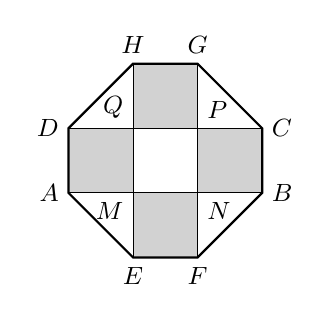
\begin{tikzpicture}[scale=0.82, every node/.style={font=\small}]
  \fill[gray!35] (-1.5,-0.5) rectangle (1.5,0.5);
  \fill[gray!35] (-0.5,-1.5) rectangle (0.5,1.5);
  % 中心正方形 MNPQ 原卷不涂阴影，照原卷留白：
  \fill[white] (-0.5,-0.5) rectangle (0.5,0.5);
  \draw[thick] (-1.5,0.5)--(-0.5,1.5)--(0.5,1.5)--(1.5,0.5)--(1.5,-0.5)--(0.5,-1.5)--(-0.5,-1.5)--(-1.5,-0.5)--cycle;
  \draw (-1.5,-0.5) rectangle (1.5,0.5);
  \draw (-0.5,-1.5) rectangle (0.5,1.5);
  \node[left] at (-1.5,0.5) {$D$};
  \node[left] at (-1.5,-0.5) {$A$};
  \node[right] at (1.5,0.5) {$C$};
  \node[right] at (1.5,-0.5) {$B$};
  \node[above] at (-0.5,1.5) {$H$};
  \node[above] at (0.5,1.5) {$G$};
  \node[below] at (-0.5,-1.5) {$E$};
  \node[below] at (0.5,-1.5) {$F$};
  \node[below left] at (-0.5,-0.5) {$M$};
  \node[below right] at (0.5,-0.5) {$N$};
  \node[above right] at (0.5,0.5) {$P$};
  \node[above left] at (-0.5,0.5) {$Q$};
\end{tikzpicture}
\end{center}

\begin{enumerate}[label=(\arabic*)]
\item 设 $DQ$ 长为 $y$（单位：m），用 $x$ 表示 $y$，并求出 $x$ 的取值范围；
\item $AD$ 取何值时可使总造价最低，并求出最低造价.
\end{enumerate}

\ifanswer
\solbegin
\stepm{(1)}{设 $AD=x\text{m}$（$x>0$），$DQ=y\text{m}$（$y>0$），}
\step{因为十字形区域总面积为 $200\text{m}^2$，所以 $4xy+x^2=200$，}
\step{解得 $y=\dfrac{200-x^2}{4x}=\dfrac{50}{x}-\dfrac{x}{4}$，}
\step{因为 $x>0$，$y>0$，所以 $y=\dfrac{200-x^2}{4x}>0$，解得 $0<x<10\sqrt2$，}
\step{所以 $y=\dfrac{50}{x}-\dfrac{x}{4}$，$0<x<10\sqrt2$；}
\stepm{(2)}{中心正方形 $MNPQ$ 区域，造价为 $2100$ 元$/\text{m}^2$，}
\step{中心正方形 $MNPQ$ 面积为 $S_1=x^2$，造价为 $W_1=2100\times S_1=2100x^2$；}
\step{周围四个矩形区域（图中阴影部分）铺设透水地砖，造价为 $105$ 元$/\text{m}^2$，}
\step{四个矩形的总面积为 $S_2=4xy=4x\left(\dfrac{50}{x}-\dfrac{x}{4}\right)=200-x^2$，}
\step{造价为 $W_2=105\times S_2=105(200-x^2)=21000-105x^2$；}
\step{四个三角形区域种植耐旱固碳植物，助力碳中和，造价为 $40$ 元$/\text{m}^2$，}
\step{四个三角形的总面积为 $S_3=4\times\dfrac12y^2=2\left(\dfrac{50}{x}-\dfrac{x}{4}\right)^2
=\dfrac{5000}{x^2}-50+\dfrac{x^2}{8}$，}
\step{造价为 $W_3=40\times S_3=40\left(\dfrac{5000}{x^2}-50+\dfrac{x^2}{8}\right)
=\dfrac{200000}{x^2}-2000+5x^2$；}
\step{设总造价为 $W$（单位：元），}
\step{则总造价为 $W=W_1+W_2+W_3$}
\step{$=2100x^2+21000-105x^2+\dfrac{200000}{x^2}-2000+5x^2$}
\step{$=2000x^2+\dfrac{200000}{x^2}+19000$，}
\step{又 $2000x^2+\dfrac{200000}{x^2}\geqslant2\sqrt{2000x^2\times\dfrac{200000}{x^2}}=2\times20000=40000$，}
\step{当且仅当 $2000x^2=\dfrac{200000}{x^2}$，即 $x=\sqrt{10}$（在 $x$ 的范围内）时取等号，}
\step{所以 $W=2000x^2+\dfrac{200000}{x^2}+19000\geqslant59000$，当 $x=\sqrt{10}$ 时取等号，}
\step{故当 $AD$ 的长为 $\sqrt{10}$ 时，总造价最低，为 $59000$ 元.}
\solend

\fi

\ansspace[8]

\item 对于实数 $a$、$b$、$c$，若 $|a-c|<|b-c|$，则称 $a$ 比 $b$ 更接近于 $c$. 现已知 $p$、$q$ 都是正有理数.

\begin{enumerate}[label=(\arabic*)]
\item 证明：$\sqrt3$ 必在 $\dfrac pq$ 和 $\dfrac{p+3q}{p+q}$ 之间；
\item 试问 $\dfrac pq$ 和 $\dfrac{p+3q}{p+q}$ 这两个数，哪一个更接近于 $\sqrt3$？说明你的理由；
\item 请你再写出一个有理数，使得它的值比 $\dfrac pq$ 和 $\dfrac{p+3q}{p+q}$ 的值更接近于 $\sqrt3$，并说明你的理由.
\end{enumerate}

\ifanswer
\solbegin
\stepm{(1)}{设 $a=\dfrac pq$（$a$ 为正有理数），则需证 $\sqrt3$ 在 $a$ 和 $\dfrac{a+3}{a+1}$（即 $\dfrac{p+3q}{p+q}$）之间.}
\step{当 $a>\sqrt3$ 时，计算 $a-\dfrac{a+3}{a+1}$ 得 $a-\dfrac{a+3}{a+1}=\dfrac{a(a+1)-(a+3)}{a+1}=\dfrac{a^2-3}{a+1}$，}
\step{$a>\sqrt3$，则 $a^2-3>0$，故 $a>\dfrac{a+3}{a+1}$；}
\step{再计算 $\dfrac{a+3}{a+1}-\sqrt3$ 得 $\dfrac{a+3}{a+1}-\sqrt3=\dfrac{(1-\sqrt3)(a-\sqrt3)}{a+1}$，}
\step{$1-\sqrt3<0$，$a-\sqrt3>0$，$a+1>0$，}
\step{故 $\dfrac{a+3}{a+1}-\sqrt3<0$，即 $\dfrac{a+3}{a+1}<\sqrt3$，从而 $\dfrac{a+3}{a+1}<\sqrt3<a$；}
\step{当 $a<\sqrt3$ 时，同理可得 $a<\dfrac{a+3}{a+1}$ 且 $\dfrac{a+3}{a+1}>\sqrt3$，即 $a<\sqrt3<\dfrac{a+3}{a+1}$，}
\step{综上，$\sqrt3$ 必在 $\dfrac pq$ 和 $\dfrac{p+3q}{p+q}$ 之间；}
\stepm{(2)}{设 $a=\dfrac pq$，$b=\dfrac{p+3q}{p+q}=\dfrac{a+3}{a+1}$，比较 $|a-\sqrt3|$ 与 $|b-\sqrt3|$，}
\step{由（1）得 $(a-\sqrt3)(b-\sqrt3)<0$，}
\step{$\dfrac{|b-\sqrt3|}{|a-\sqrt3|}
=\left|\dfrac{b-\sqrt3}{a-\sqrt3}\right|
=\dfrac{\left|\dfrac{(1-\sqrt3)(a-\sqrt3)}{a+1}\right|}{|a-\sqrt3|}
=\dfrac{\sqrt3-1}{a+1}$，}
\step{$a>0$，$a+1>1$，$\sqrt3-1<1$，故 $\dfrac{\sqrt3-1}{a+1}<1$，即 $|b-\sqrt3|<|a-\sqrt3|$，}
\step{即 $\dfrac{p+3q}{p+q}$ 比 $\dfrac pq$ 更接近于 $\sqrt3$；}
\stepm{(3)}{$\dfrac{2p+3q}{p+2q}$，理由：}
\step{设 $b=\dfrac{p+3q}{p+q}$，新数 $c=\dfrac{b+3}{b+1}=\dfrac{2p+3q}{p+2q}$，}
\step{由（1）得 $(b-\sqrt3)(c-\sqrt3)<0$，}
\step{$c-\sqrt3=\dfrac{b+3}{b+1}-\sqrt3=\dfrac{(1-\sqrt3)(b-\sqrt3)}{b+1}$，}
\step{则 $\dfrac{|c-\sqrt3|}{|b-\sqrt3|}
=\left|\dfrac{c-\sqrt3}{b-\sqrt3}\right|
=\dfrac{\left|\dfrac{(1-\sqrt3)(b-\sqrt3)}{b+1}\right|}{|b-\sqrt3|}
=\dfrac{\sqrt3-1}{b+1}$，}
\step{$b>0$，$b+1>1$，$0<\sqrt3-1<1$，故 $\dfrac{\sqrt3-1}{b+1}<1$，即 $|c-\sqrt3|<|b-\sqrt3|$，}
\step{即 $\dfrac{2p+3q}{p+2q}$ 比 $\dfrac{p+3q}{p+q}$ 更接近于 $\sqrt3$，故 $c$ 更接近 $\sqrt3$.}
\solend

\fi

\ansspace*[10]

\end{enumerate}

\end{document}
"
%
% 原始材料是微信公众号图文（公众号“魔都数学加油站”，作者“破晓”，2026-10-02 17:56 发布，
% 连载“27学年高一45”，原文标题“27学年高一45——2026-2027年上海市交附闵行高一上国庆作业2”，
% https://mp.weixin.qq.com/s/1xdCtzH-3Il0jJrz3saiPA），正文为 10 张 PNG 页。
% 第 01—06、09 页为 4762×6735；第 07、08、10 页为 2560×3620（同一篇各页原图分辨率不一致）。
% 原文本身是一份讲评版：第 3—21 题均照原卷保留题目与题下解析；第 13 题原卷把答案 C 印在括号中。
% 题目、选项、答案与解析均照原卷录入，未改内容；卷面的粉色斜水印及页脚不录入。
%
% 卷首标题：原卷印作“2026-2027 年交附闵行高一上国庆作业 2”（公众号标题里的“上海市”
% 三字卷面标题行没有，本稿照卷面），年份区间按全稿惯例排 en dash，前缀照原卷保留“年”。
%
% 与原卷的排版差异：
%   ① 原卷印有“一、填空题”“二、选择题”“三、解答题”三节标题，本稿照原卷分节，
%      只把标题改排成全稿统一的“大节标题”样式；
%   ② 第 13 题原卷在题干括号内直接印答案 C，本稿按全稿样式将括号留空、答案移入答案版的 \ans{}；
%   ③ 原卷填空横线及选择题答案括号均按全稿样式排版，填空横线统一用 \blankline[4.4em]；
%   ④ 原卷第 20 题配有十字形广场示意图，本稿在源码中用 TikZ 重绘，图中区域、边界及点名照原卷。
%   ⑤ 原卷未印副标题，本稿按本卷实际涉及的知识模块补出“集合与常用逻辑用语、不等式”。
%
% 原卷存疑/错误（均照抄原卷、未改，见对应题目处上方注释）：
%   ① 第 11 题解析原卷印"所以 p=3+9=12，又 12,15∉A，所以 12,15∉B"，与 A∪\overline{B} 的条件
%      及后文 B 的根为 6、9 均一致，无矛盾，本稿照录（早前记录的"∈B／前后矛盾"系本稿误读）；
%   ② 第 15 题题干与解析均按原卷印 ac<0，解析"因为 a<b<c，且 ac<0，所以 a<0，c>0"与题设一致，
%      无矛盾（早前记录的"abc<0／解析冲突"系本稿误读题干所致）；本稿照录原卷答案与解析。
%   ③ 第 20 题原卷各数（造价 2100 元/m^2、W_1=2100x^2、合并式 2000x^2+200000/x^2+19000、
%      末句 59000 元）经复核自洽，无矛盾（早前记录的"W_1=200x^2／末句 5900 元"系本稿误录）；本稿照录。
%   ④ 第 18(2) 题 a=-1 时 A=B=(-1,1)，不满足“B 是 A 的真子集”，故原解析给出的 a≤-1 应为 a<-1；
%   ⑤ 第 19(2) 题原卷用"{c|0<c<1}∩{c|c<-2√3/3 或 c>2√3/3}=∅"论证"不等式①、②中至多有一个恒成立"，
%      论证成立（早前记录的"区间并集留有间隙"系本稿误录解析所致）；本稿照录原卷。
%
\documentclass[a4paper,11pt]{article}
\usepackage{common}

\begin{document}

\examtitlest[3]{2026--2027 年交附闵行高一上国庆作业 2}{集合与常用逻辑用语、不等式}

\bigsec{一、填空题}

\begin{enumerate}
\setcounter{enumi}{2}

\item 满足 $A\cup\{-1,1\}=\{-1,0,1\}$ 的集合 $A$ 共有 \blankline[4.4em] 个.

\ifanswer
\solbegin
\step{集合可能为 $\{0\}$、$\{0,1\}$、$\{0,-1\}$、$\{0,1,-1\}$，共有 $4$ 个.}
\solend

\fi

\item 设 $x\in\R$，则“$x+\dfrac1x>2$”是“$x\neq1$”的 \blankline[4.4em] 条件.

\ifanswer
\solbegin
\step{$x+\dfrac1x>2\Longleftrightarrow x>0$ 且 $x\neq1$，故为充分不必要条件.}
\solend

\fi

\item 已知集合 $A=\{x\mid|x-1|<a\}$，$B=\{-4,3\}$，若 $A\cap B=\varnothing$，则 $a$ 的最大值为 \blankline[4.4em].

\ifanswer
\solbegin
\step{$A=\{x\mid -a<x-1<a\}=\{x\mid1-a<x<1+a\}$，$B=\{-4,3\}$，且 $A\cap B=\varnothing$，}
\step{$A=\varnothing$ 时，$1-a\geqslant1+a$，解得 $a\leqslant0$，满足 $A\cap B=\varnothing$；}
\step{若 $-4\in A$，则 $1-a<-4<1+a$，解得 $a>5$；}
\step{若 $3\in A$，则 $1-a<3<1+a$，解得 $a>2$，}
\step{因为 $A\cap B=\varnothing$，所以 $-4\notin A$ 且 $3\notin A$，所以 $a\leqslant5$ 且 $a\leqslant2$，所以 $a\leqslant2$，}
\step{综上，$a$ 的最大值为 $2$.}
\solend

\fi

\item 设 $x\in\R$，方程 $|x-1|+|2x-1|=|3x-2|$ 的解集为 \blankline[4.4em].

\ifanswer
\solbegin
\step{因为 $|x-1|+|2x-1|\geqslant|(x-1)+(2x-1)|=|3x-2|$，}
\step{当且仅当 $(x-1)(2x-1)\geqslant0$，解得 $x\leqslant\dfrac12$ 或 $x\geqslant1$，}
\step{故方程 $|x-1|+|2x-1|=|3x-2|$ 的解集为 $\left(-\infty,\dfrac12\right]\cup[1,+\infty)$.}
\solend

\fi

\item 已知 $a$、$b\in\R$，且 $3a+2b=1$，则 $8^a+4^b$ 最小值为 \blankline[4.4em].

\ifanswer
\solbegin
% 注：原卷本行与上行均作“$8^a+4^b$ 最小值为”，“最小值”前无“的”，原卷如此，照录未改。
\step{因为 $3a+2b=1$，所以 $8^a+4^b=2^{3a}+2^{2b}\geqslant2\sqrt{2^{3a+2b}}=2\sqrt2$，}
\step{当且仅当 $3a=2b$ 时取等号，故 $8^a+4^b$ 最小值为 $2\sqrt2$.}
\solend

\fi

\item 已知 $a>0$，$b>0$，且 $a+2b+ab=30$，则 $2a+b$ 的最小值为 \blankline[4.4em].

\ifanswer
\solbegin
\step{由 $a+2b+ab=30$，得 $(a+2)(b+1)=32$.}
\step{因为 $a>0$，$b>0$，所以 $a+2>0$，$b+1>0$，}
\step{所以 $2a+b=2(a+2)+(b+1)-5\geqslant2\sqrt{2\times32}-5=11$，}
\step{当且仅当 $2(a+2)=(b+1)$，即 $a=2$，$b=7$ 时取等号，}
\step{所以 $2a+b$ 的最小值为 $11$.}
\solend

\fi

\item 已知 $A=\{x\mid x^2+px+1=0\}$，$M=\{x\mid x>0\}$，若 $A\cap M=\varnothing$，则实数 $p$ 的取值范围为 \blankline[4.4em].

\ifanswer
\solbegin
\step{①当 $A=\varnothing$ 时，$\Delta=p^2-4<0$，所以 $-2<p<2$，此时满足 $A\cap M=\varnothing$；}
\step{②当 $A\neq\varnothing$ 时，$\Delta=p^2-4\geqslant0$，$p\geqslant2$ 或 $p\leqslant-2$，}
\step{因为 $M=\{x\mid x>0\}$，$A\cap M=\varnothing$，由韦达定理得 $\begin{cases}-p\leqslant0\\1>0\end{cases}$，解得 $p\geqslant0$，}
\step{所以 $p\geqslant2$，}
\step{由①②综合得 $p>-2$，故实数 $p$ 的取值范围为 $(-2,+\infty)$.}
\solend

\fi

\item 已知集合 $A=[t,t+1]\cup[t+3,t+6]$，其中 $t>0$. 若存在正数 $\lambda$，使得对任意 $a\in A$，都有 $\dfrac{\lambda}{a}\in A$，则 $t$ 的取值集合为 \blankline[4.4em].

\ifanswer
\solbegin
\step{因为 $0\notin A$，$t>0$，所以 $a\in[t,t+1]\cup[t+3,t+6]$，}
\step{则 $\dfrac1a\in\left[\dfrac1{t+6},\dfrac1{t+3}\right]\cup\left[\dfrac1{t+1},\dfrac1t\right]$，}
\step{又因为 $\lambda>0$，所以 $\dfrac{\lambda}{a}\in\left[\dfrac{\lambda}{t+6},\dfrac{\lambda}{t+3}\right]\cup\left[\dfrac{\lambda}{t+1},\dfrac{\lambda}{t}\right]$，}
\step{因为 $\dfrac{\lambda}{a}\in A$，所以 $\begin{cases}\dfrac{\lambda}{t+6}\geqslant t\\[3pt]\dfrac{\lambda}{t+3}\leqslant t+1\end{cases}$ 且 $\begin{cases}\dfrac{\lambda}{t+1}\geqslant t+3\\[3pt]\dfrac{\lambda}{t}\leqslant t+6\end{cases}$，}
% 注：原卷本行两个不等式组印作“$t(t+6)\leqslant\lambda\leqslant t(t+6)$”与
%     “$(t+1)(t+3)\leqslant\lambda\leqslant(t+1)(t+3)$”（两侧同式），与上行两式推导不合，系原卷笔误；
%     原卷如此，照录未改。
\step{得 $\begin{cases}t(t+6)\leqslant\lambda\leqslant t(t+6)\\[3pt](t+1)(t+3)\leqslant\lambda\leqslant(t+1)(t+3)\end{cases}$，所以 $\lambda=t(t+6)=(t+1)(t+3)$，}
\step{解得 $t=\dfrac32$，取值集合为 $\left\{\dfrac32\right\}$.}
\solend

\fi

\item 已知全集 $U=\{x\mid x=3n,1\leqslant n\leqslant5\ \text{且}\ n\in\N\}$，$A=\{x\mid x^2-px+27=0,p\in\N\}$，
$B=\{x\mid x^2-15x+q=0,q\in\N\}$，且 $A\cup\overline{B}=\{3,9,12,15\}$，则 $p+q$ 的值为 \blankline[4.4em].

\ifanswer
\solbegin
\step{因为全集 $U=\{3,6,9,12,15\}$，$A\cup\overline{B}=\{3,9,12,15\}$，}
\step{所以 $3$、$9$、$12$、$15$ 中可能有两个属于 $A$，}
\step{因为 $A$ 中的方程 $x^2-px+27=0$ 中，两根之积 $x_1x_2=27$，所以 $3$、$9\in A$，}
\step{所以 $p=3+9=12$，又 $12$、$15\notin A$，所以 $12$、$15\notin B$，}
\step{因为 $B$ 中的方程 $x^2-15x+q=0$ 中，两根之和 $x_3+x_4=15$，所以 $6$、$9\in B$，}
\step{则 $q=6\times9=54$，所以 $p+q=66$.}
\solend

\fi

\item 若关于 $x$ 的不等式 $|x-2k|+|x-3k|<4k$ 共有 $2025$ 个整数解，则实数 $k$ 的取值范围为 \blankline[4.4em].

\ifanswer
\solbegin
\step{显然 $k>0$，由 $|x-2k|+|x-3k|<4k$，得 $\dfrac{k}{2}<x<\dfrac{9k}{2}$，}
\step{因为该不等式共有 $2025$ 个整数解，所以 $2024<\dfrac{9k}{2}-\dfrac{k}{2}\leqslant2026$，}
\step{解得 $506<k\leqslant506.5$，}
\step{由 $\dfrac{k}{2}\in(253,253.25]$，得这 $2025$ 个整数解只能为 $254,255,256,\cdots,2278$，}
\step{所以 $2278<\dfrac{9k}{2}\leqslant2279$，解得 $506\dfrac29<k\leqslant506\dfrac49$，结合 $506<k\leqslant506.5$，}
\step{得 $k$ 的取值范围是 $\left(506\dfrac29,506\dfrac49\right]$.}
\solend

\fi

\end{enumerate}

\bigsec{二、选择题}

\begin{enumerate}
\setcounter{enumi}{12}

\item 已知 $a,b\in\R$，且 $ab\neq0$，则下列结论恒成立的是\mbox{（\quad）}

\keepwithprev
A. $a+b\geqslant2\sqrt{ab}$\qquad
B. $\left(\dfrac{a+b}{2}\right)^2>ab$\qquad
C. $\left|\dfrac ab+\dfrac ba\right|\geqslant2$\qquad
D. $a^2+b^2>2ab$

\ans{$C$}

\item 如果 $a^{2025}+b^{2025}=0$，那么一定有\mbox{（\quad）}

\keepwithprev
A. $(|a|+|b|)^{2025}=0$\qquad
B. $(a-b)^{2025}=0$\qquad
C. $(a\cdot b)^{2025}=0$\qquad
D. $(a+b)^{2025}=0$

\ans{$D$}

\ifanswer
\solbegin
\step{由 $a^{2025}+b^{2025}=0$，得 $a^{2025}=-b^{2025}=(-b)^{2025}$，则 $\left(a^{2025}\right)^{\frac{1}{2025}}=\left[(-b)^{2025}\right]^{\frac{1}{2025}}$，}
\step{即 $a=-b$，即 $a+b=0$，故 $(a+b)^{2025}=0$，故 D 符合题意；}
\step{对于 A，若取 $a=1$，$b=-1$，则 $(|a|+|b|)^{2025}=2^{2025}\neq0$，故 A 不合题意；}
\step{对于 B，若取 $a=1$，$b=-1$，则 $(a-b)^{2025}=2^{2025}\neq0$，故 B 不合题意；}
\step{对于 C，若取 $a=1$，$b=-1$，则 $(a\cdot b)^{2025}=(-1)^{2025}=-1\neq0$，故 C 不合题意；}
\step{故选 D.}
\solend

\fi

\item 已知 $a$、$b$、$c$ 满足 $a<b<c$，且 $ac<0$，那么下列各式中一定成立的是\mbox{（\quad）}

\keepwithprev
A. $\dfrac1a>\dfrac1c$\qquad
B. $ab^2<cb^2$\qquad
C. $ac<bc$\qquad
D. $a+c>2b$

\ans{$C$}

\ifanswer
\solbegin
\step{因为 $a<b<c$，且 $ac<0$，所以 $a<0$，$c>0$，}
\step{对于 A，$\dfrac1a<0<\dfrac1c$，故 A 错误；}
\step{对于 B，当 $b=0$ 时，$ab^2=cb^2$，故 B 错误；}
\step{对于 C，$ac<bc$ 可化为 $(a-b)c<0$，因为 $a<b$，所以 $a-b<0$，}
\step{又因为 $c>0$，所以 $(a-b)c<0$，所以 C 正确；}
\step{对于 D，设 $a=-2$，$b=0$，$c=1$，则 $a+c<2b$，故 D 错误.}
\step{故选 C.}
\solend

\fi

\item 对于 $a\in\R$，设集合 $A=\left\{x\mid\dfrac{(x^2-6x+a)(x-1)}{x+a}=0\right\}$，记 $A$ 的所有元素之和为 $S(a)$，
所有元素之积为 $T(a)$，则下列说法中，正确的是\mbox{（\quad）}

\keepwithprev
A. 不存在实数 $a$，使得 $S(a)=6$\qquad
B. 存在实数 $a$，使得 $T(a)=9$

C. 存在无数实数 $a$，使得 $S(a)=7$\qquad
D. 若 $T(a)=3$，则 $a=3$

\ans{$C$}

\ifanswer
\solbegin
\step{要使 $\dfrac{(x^2-6x+a)(x-1)}{x+a}=0$，只需 $(x^2-6x+a)(x-1)=0$ 且 $x+a\neq0$，}
\step{由 $(x^2-6x+a)(x-1)=0$ 得 $x^2-6x+a=0$ 或 $x-1=0$，}
\step{对于一元二次方程 $x^2-6x+a=0$，其判别式 $\Delta=36-4a$，}
\step{当 $\Delta=0$，即 $a=9$ 时，集合 $A=\{1,3\}$，$S(a)=4$，$T(a)=3$；}
\step{当 $\Delta<0$，即 $a>9$ 时，集合 $A=\{1\}$，$S(a)=T(a)=1$；}
\step{当 $\Delta>0$，即 $a<9$ 时，一元二次方程 $x^2-6x+a=0$ 的解为 $x=3\pm\sqrt{9-a}$，}
\step{①当 $a=0$ 时，$x\neq0$，则集合 $A=\{1,6\}$，则 $S(a)=7$，$T(a)=6$，}
\step{②当 $a=-7$ 时，$x\neq7$，则集合 $A=\{-1,1\}$，则 $S(a)=0$，$T(a)=-1$，}
% 注：下一行集合 A 原卷印作 {-1,1}（按 a=-1 代入 x^2-6x-1=0 应得 3±√10，原卷如此，照录未改）。
\step{③当 $a=-1$ 时，$x\neq1$，则集合 $A=\{-1,1\}$，则 $S(a)=6$，$T(a)=-1$，}
\step{④当 $a=5$ 时，$x\neq-5$，则集合 $A=\{1,5\}$，则 $S(a)=6$，$T(a)=5$，}
\step{⑤当 $a\neq5,0,-1,-7$ 时，集合 $A=\{1,3-\sqrt{9-a},3+\sqrt{9-a}\}$，}
\step{则 $S(a)=7$，$T(a)=a$.}
\step{选项 A，当 $a=5$ 时，$S(a)=6$，所以 A 错误；}
\step{选项 B，$T(a)$ 的可能值为 $-1,1,3,5,6,a$（$a<9$），无 $T(a)=9$，所以 B 错误；}
\step{选项 C，当 $a<9$，且 $a\neq5,-1,-7$ 时，$S(a)=7$，有无数个 $a$ 满足，所以 C 正确；}
\step{选项 D，当 $T(a)=3$ 时，有 $a=3$ 和 $a=9$ 满足，所以 D 错误.}
\step{故选 C.}
\solend

\fi

\end{enumerate}

\bigsec{三、解答题}

\begin{enumerate}
\setcounter{enumi}{16}

\item 已知 $a\in\R$，关于 $x$ 的不等式 $|x+1|+|x-1|>a^2-5a+4$.

\begin{enumerate}[label=(\arabic*)]
\item 当 $a=0$ 时，求不等式的解集；
\item 若不等式的解集为 $\R$，求 $a$ 的取值范围.
\end{enumerate}

\ifanswer
\solbegin
\stepm{(1)}{当 $a=0$ 时，不等式为 $|x+1|+|x-1|>4$，}
\step{又 $|x+1|+|x-1|=\begin{cases}2x,&x\geqslant1\\2,&-1<x<1\\-2x,&x\leqslant-1\end{cases}$，}
\step{则 $|x+1|+|x-1|>4$ 的解为 $x>2$ 或 $x<-2$，}
\step{即不等式的解集为 $(-\infty,-2)\cup(2,+\infty)$；}
\stepm{(2)}{不等式 $|x+1|+|x-1|>a^2-5a+4$ 的解集为 $\R$，}
\step{则 $(|x+1|+|x-1|)_{\min}>a^2-5a+4$，}
\step{又 $(|x+1|+|x-1|)_{\min}=2$，当且仅当 $-1\leqslant x\leqslant1$ 时取得，即 $a^2-5a+4<2$，}
\step{即 $a^2-5a+2<0$，即 $\dfrac{5-\sqrt{17}}2<a<\dfrac{5+\sqrt{17}}2$，}
\step{即 $a$ 的取值范围为 $\left(\dfrac{5-\sqrt{17}}2,\dfrac{5+\sqrt{17}}2\right)$.}
\solend

\fi

\ansspace[6]

\item 已知集合 $A=\{x\mid(x-a)(x-a^2)<0\}$，集合 $B=\left\{x\mid\dfrac{2x}{x-1}<1\right\}$，命题 $p:x\in A$，命题 $q:x\in B$.

\begin{enumerate}[label=(\arabic*)]
\item 当实数 $a$ 为何值时，$A=B$；
\item 若 $q$ 是 $p$ 的充分不必要条件，求实数 $a$ 的取值范围.
\end{enumerate}

\ifanswer
\solbegin
\stepm{(1)}{由 $\dfrac{2x}{x-1}<1$ 得 $\dfrac{2x}{x-1}-1=\dfrac{x+1}{x-1}<0$，解得 $-1<x<1$，即 $B=\{x\mid-1<x<1\}$，}
\step{因为 $A=\{x\mid(x-a)(x-a^2)<0\}$，$A=B$，所以 $\begin{cases}a=-1\\a^2=1\end{cases}$，解得 $a=-1$；}
\stepm{(2)}{若 $q$ 是 $p$ 的充分不必要条件，则 $B\subset A$，}
\step{当 $a^2=a$，即 $a=0$ 或 $a=1$ 时，$A=\varnothing$，显然不符合题意；}
\step{当 $a^2>a$，即 $a>1$ 或 $a<0$ 时，$A=(a,a^2)$，则 $\begin{cases}a\leqslant-1\\a^2\geqslant1\\a>1\ \text{或}\ a<0\end{cases}$，}
% 注：a=-1 时 A=(-1,1)=B，不是 B 的真子集；原解析用 B⊂A 但答案含 -1，照录。
\step{前两等号不能同时取得，解得 $a\leqslant-1$；}
\step{当 $a^2<a$，即 $0<a<1$ 时，$A=(a^2,a)$，显然不符合题意，}
\step{故 $a$ 的范围为 $\{a\mid a\leqslant-1\}$.}
\solend

\fi

\ansspace[6]

\item 已知不等式① $x^2+2cx+c>0$，② $x^2+cx+c^2-1>0$，其中 $c$ 是实数.

\begin{enumerate}[label=(\arabic*)]
\item 若 $1$ 是不等式②的一个解，求实数 $c$ 的取值范围；
\item 证明：不等式①、②中至多有一个恒成立.
\end{enumerate}

\ifanswer
\solbegin
\stepm{(1)}{已知不等式① $x^2+2cx+c>0$，② $x^2+cx+c^2-1>0$，}
\step{又 $1$ 是不等式②的一个解，则 $1+c+c^2-1>0$，}
\step{则 $c^2+c>0$，则 $c<-1$ 或 $c>0$，则 $c$ 的取值范围为 $(-\infty,-1)\cup(0,+\infty)$；}
\stepm{(2)}{若不等式①恒成立，则 $\Delta=4c^2-4c<0$，则 $0<c<1$，}
\step{若不等式②恒成立，则 $\Delta=c^2-4(c^2-1)=4-3c^2<0$，}
\step{则 $c<-\dfrac{2\sqrt3}{3}$ 或 $c>\dfrac{2\sqrt3}{3}$，}
\step{又 $\{c\mid 0<c<1\}\cap\left\{c\mid c<-\dfrac{2\sqrt3}{3}\ \text{或}\ c>\dfrac{2\sqrt3}{3}\right\}=\varnothing$，}
\step{则不存在实数 $c$ 使得不等式①、②同时恒成立，}
\step{则不等式①、②中至多有一个恒成立.}
\solend

\fi

\ansspace[6]

\item 为践行“科技强国”战略，某社区计划建造一座融合智慧节能技术的八边形休闲广场，其中两个相同的矩形 $ABCD$ 和 $EFGH$ 构成的十字形区域总面积为 $200\text{m}^2$. 中心正方形 $MNPQ$ 区域将安装国产太阳能光伏板（兼具休憩遮阳功能），造价为 $2100$ 元$/\text{m}^2$；周围四个矩形区域（图中阴影部分）铺设透水地砖，造价为 $105$ 元$/\text{m}^2$；再在四个三角形区域种植耐旱固碳植物，助力碳中和，造价为 $40$ 元$/\text{m}^2$. 设总造价为 $W$（单位：元），$AD=x$（单位：m）.

\begin{center}
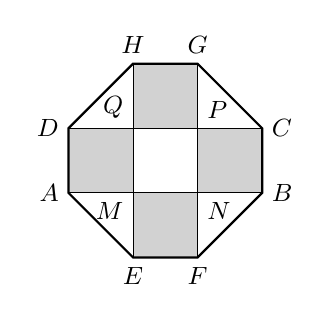
\begin{tikzpicture}[scale=0.82, every node/.style={font=\small}]
  \fill[gray!35] (-1.5,-0.5) rectangle (1.5,0.5);
  \fill[gray!35] (-0.5,-1.5) rectangle (0.5,1.5);
  % 中心正方形 MNPQ 原卷不涂阴影，照原卷留白：
  \fill[white] (-0.5,-0.5) rectangle (0.5,0.5);
  \draw[thick] (-1.5,0.5)--(-0.5,1.5)--(0.5,1.5)--(1.5,0.5)--(1.5,-0.5)--(0.5,-1.5)--(-0.5,-1.5)--(-1.5,-0.5)--cycle;
  \draw (-1.5,-0.5) rectangle (1.5,0.5);
  \draw (-0.5,-1.5) rectangle (0.5,1.5);
  \node[left] at (-1.5,0.5) {$D$};
  \node[left] at (-1.5,-0.5) {$A$};
  \node[right] at (1.5,0.5) {$C$};
  \node[right] at (1.5,-0.5) {$B$};
  \node[above] at (-0.5,1.5) {$H$};
  \node[above] at (0.5,1.5) {$G$};
  \node[below] at (-0.5,-1.5) {$E$};
  \node[below] at (0.5,-1.5) {$F$};
  \node[below left] at (-0.5,-0.5) {$M$};
  \node[below right] at (0.5,-0.5) {$N$};
  \node[above right] at (0.5,0.5) {$P$};
  \node[above left] at (-0.5,0.5) {$Q$};
\end{tikzpicture}
\end{center}

\begin{enumerate}[label=(\arabic*)]
\item 设 $DQ$ 长为 $y$（单位：m），用 $x$ 表示 $y$，并求出 $x$ 的取值范围；
\item $AD$ 取何值时可使总造价最低，并求出最低造价.
\end{enumerate}

\ifanswer
\solbegin
\stepm{(1)}{设 $AD=x\text{m}$（$x>0$），$DQ=y\text{m}$（$y>0$），}
\step{因为十字形区域总面积为 $200\text{m}^2$，所以 $4xy+x^2=200$，}
\step{解得 $y=\dfrac{200-x^2}{4x}=\dfrac{50}{x}-\dfrac{x}{4}$，}
\step{因为 $x>0$，$y>0$，所以 $y=\dfrac{200-x^2}{4x}>0$，解得 $0<x<10\sqrt2$，}
\step{所以 $y=\dfrac{50}{x}-\dfrac{x}{4}$，$0<x<10\sqrt2$；}
\stepm{(2)}{中心正方形 $MNPQ$ 区域，造价为 $2100$ 元$/\text{m}^2$，}
\step{中心正方形 $MNPQ$ 面积为 $S_1=x^2$，造价为 $W_1=2100\times S_1=2100x^2$；}
\step{周围四个矩形区域（图中阴影部分）铺设透水地砖，造价为 $105$ 元$/\text{m}^2$，}
\step{四个矩形的总面积为 $S_2=4xy=4x\left(\dfrac{50}{x}-\dfrac{x}{4}\right)=200-x^2$，}
\step{造价为 $W_2=105\times S_2=105(200-x^2)=21000-105x^2$；}
\step{四个三角形区域种植耐旱固碳植物，助力碳中和，造价为 $40$ 元$/\text{m}^2$，}
\step{四个三角形的总面积为 $S_3=4\times\dfrac12y^2=2\left(\dfrac{50}{x}-\dfrac{x}{4}\right)^2
=\dfrac{5000}{x^2}-50+\dfrac{x^2}{8}$，}
\step{造价为 $W_3=40\times S_3=40\left(\dfrac{5000}{x^2}-50+\dfrac{x^2}{8}\right)
=\dfrac{200000}{x^2}-2000+5x^2$；}
\step{设总造价为 $W$（单位：元），}
\step{则总造价为 $W=W_1+W_2+W_3$}
\step{$=2100x^2+21000-105x^2+\dfrac{200000}{x^2}-2000+5x^2$}
\step{$=2000x^2+\dfrac{200000}{x^2}+19000$，}
\step{又 $2000x^2+\dfrac{200000}{x^2}\geqslant2\sqrt{2000x^2\times\dfrac{200000}{x^2}}=2\times20000=40000$，}
\step{当且仅当 $2000x^2=\dfrac{200000}{x^2}$，即 $x=\sqrt{10}$（在 $x$ 的范围内）时取等号，}
\step{所以 $W=2000x^2+\dfrac{200000}{x^2}+19000\geqslant59000$，当 $x=\sqrt{10}$ 时取等号，}
\step{故当 $AD$ 的长为 $\sqrt{10}$ 时，总造价最低，为 $59000$ 元.}
\solend

\fi

\ansspace[8]

\item 对于实数 $a$、$b$、$c$，若 $|a-c|<|b-c|$，则称 $a$ 比 $b$ 更接近于 $c$. 现已知 $p$、$q$ 都是正有理数.

\begin{enumerate}[label=(\arabic*)]
\item 证明：$\sqrt3$ 必在 $\dfrac pq$ 和 $\dfrac{p+3q}{p+q}$ 之间；
\item 试问 $\dfrac pq$ 和 $\dfrac{p+3q}{p+q}$ 这两个数，哪一个更接近于 $\sqrt3$？说明你的理由；
\item 请你再写出一个有理数，使得它的值比 $\dfrac pq$ 和 $\dfrac{p+3q}{p+q}$ 的值更接近于 $\sqrt3$，并说明你的理由.
\end{enumerate}

\ifanswer
\solbegin
\stepm{(1)}{设 $a=\dfrac pq$（$a$ 为正有理数），则需证 $\sqrt3$ 在 $a$ 和 $\dfrac{a+3}{a+1}$（即 $\dfrac{p+3q}{p+q}$）之间.}
\step{当 $a>\sqrt3$ 时，计算 $a-\dfrac{a+3}{a+1}$ 得 $a-\dfrac{a+3}{a+1}=\dfrac{a(a+1)-(a+3)}{a+1}=\dfrac{a^2-3}{a+1}$，}
\step{$a>\sqrt3$，则 $a^2-3>0$，故 $a>\dfrac{a+3}{a+1}$；}
\step{再计算 $\dfrac{a+3}{a+1}-\sqrt3$ 得 $\dfrac{a+3}{a+1}-\sqrt3=\dfrac{(1-\sqrt3)(a-\sqrt3)}{a+1}$，}
\step{$1-\sqrt3<0$，$a-\sqrt3>0$，$a+1>0$，}
\step{故 $\dfrac{a+3}{a+1}-\sqrt3<0$，即 $\dfrac{a+3}{a+1}<\sqrt3$，从而 $\dfrac{a+3}{a+1}<\sqrt3<a$；}
\step{当 $a<\sqrt3$ 时，同理可得 $a<\dfrac{a+3}{a+1}$ 且 $\dfrac{a+3}{a+1}>\sqrt3$，即 $a<\sqrt3<\dfrac{a+3}{a+1}$，}
\step{综上，$\sqrt3$ 必在 $\dfrac pq$ 和 $\dfrac{p+3q}{p+q}$ 之间；}
\stepm{(2)}{设 $a=\dfrac pq$，$b=\dfrac{p+3q}{p+q}=\dfrac{a+3}{a+1}$，比较 $|a-\sqrt3|$ 与 $|b-\sqrt3|$，}
\step{由（1）得 $(a-\sqrt3)(b-\sqrt3)<0$，}
\step{$\dfrac{|b-\sqrt3|}{|a-\sqrt3|}
=\left|\dfrac{b-\sqrt3}{a-\sqrt3}\right|
=\dfrac{\left|\dfrac{(1-\sqrt3)(a-\sqrt3)}{a+1}\right|}{|a-\sqrt3|}
=\dfrac{\sqrt3-1}{a+1}$，}
\step{$a>0$，$a+1>1$，$\sqrt3-1<1$，故 $\dfrac{\sqrt3-1}{a+1}<1$，即 $|b-\sqrt3|<|a-\sqrt3|$，}
\step{即 $\dfrac{p+3q}{p+q}$ 比 $\dfrac pq$ 更接近于 $\sqrt3$；}
\stepm{(3)}{$\dfrac{2p+3q}{p+2q}$，理由：}
\step{设 $b=\dfrac{p+3q}{p+q}$，新数 $c=\dfrac{b+3}{b+1}=\dfrac{2p+3q}{p+2q}$，}
\step{由（1）得 $(b-\sqrt3)(c-\sqrt3)<0$，}
\step{$c-\sqrt3=\dfrac{b+3}{b+1}-\sqrt3=\dfrac{(1-\sqrt3)(b-\sqrt3)}{b+1}$，}
\step{则 $\dfrac{|c-\sqrt3|}{|b-\sqrt3|}
=\left|\dfrac{c-\sqrt3}{b-\sqrt3}\right|
=\dfrac{\left|\dfrac{(1-\sqrt3)(b-\sqrt3)}{b+1}\right|}{|b-\sqrt3|}
=\dfrac{\sqrt3-1}{b+1}$，}
\step{$b>0$，$b+1>1$，$0<\sqrt3-1<1$，故 $\dfrac{\sqrt3-1}{b+1}<1$，即 $|c-\sqrt3|<|b-\sqrt3|$，}
\step{即 $\dfrac{2p+3q}{p+2q}$ 比 $\dfrac{p+3q}{p+q}$ 更接近于 $\sqrt3$，故 $c$ 更接近 $\sqrt3$.}
\solend

\fi

\ansspace*[10]

\end{enumerate}

\end{document}
"
%
% 原始材料是微信公众号图文（公众号“魔都数学加油站”，作者“破晓”，2026-10-02 17:56 发布，
% 连载“27学年高一45”，原文标题“27学年高一45——2026-2027年上海市交附闵行高一上国庆作业2”，
% https://mp.weixin.qq.com/s/1xdCtzH-3Il0jJrz3saiPA），正文为 10 张 PNG 页。
% 第 01—06、09 页为 4762×6735；第 07、08、10 页为 2560×3620（同一篇各页原图分辨率不一致）。
% 原文本身是一份讲评版：第 3—21 题均照原卷保留题目与题下解析；第 13 题原卷把答案 C 印在括号中。
% 题目、选项、答案与解析均照原卷录入，未改内容；卷面的粉色斜水印及页脚不录入。
%
% 卷首标题：原卷印作“2026-2027 年交附闵行高一上国庆作业 2”（公众号标题里的“上海市”
% 三字卷面标题行没有，本稿照卷面），年份区间按全稿惯例排 en dash，前缀照原卷保留“年”。
%
% 与原卷的排版差异：
%   ① 原卷印有“一、填空题”“二、选择题”“三、解答题”三节标题，本稿照原卷分节，
%      只把标题改排成全稿统一的“大节标题”样式；
%   ② 第 13 题原卷在题干括号内直接印答案 C，本稿按全稿样式将括号留空、答案移入答案版的 \ans{}；
%   ③ 原卷填空横线及选择题答案括号均按全稿样式排版，填空横线统一用 \blankline[4.4em]；
%   ④ 原卷第 20 题配有十字形广场示意图，本稿在源码中用 TikZ 重绘，图中区域、边界及点名照原卷。
%   ⑤ 原卷未印副标题，本稿按本卷实际涉及的知识模块补出“集合与常用逻辑用语、不等式”。
%
% 原卷存疑/错误（均照抄原卷、未改，见对应题目处上方注释）：
%   ① 第 11 题解析原卷印"所以 p=3+9=12，又 12,15∉A，所以 12,15∉B"，与 A∪\overline{B} 的条件
%      及后文 B 的根为 6、9 均一致，无矛盾，本稿照录（早前记录的"∈B／前后矛盾"系本稿误读）；
%   ② 第 15 题题干与解析均按原卷印 ac<0，解析"因为 a<b<c，且 ac<0，所以 a<0，c>0"与题设一致，
%      无矛盾（早前记录的"abc<0／解析冲突"系本稿误读题干所致）；本稿照录原卷答案与解析。
%   ③ 第 20 题原卷各数（造价 2100 元/m^2、W_1=2100x^2、合并式 2000x^2+200000/x^2+19000、
%      末句 59000 元）经复核自洽，无矛盾（早前记录的"W_1=200x^2／末句 5900 元"系本稿误录）；本稿照录。
%   ④ 第 18(2) 题 a=-1 时 A=B=(-1,1)，不满足“B 是 A 的真子集”，故原解析给出的 a≤-1 应为 a<-1；
%   ⑤ 第 19(2) 题原卷用"{c|0<c<1}∩{c|c<-2√3/3 或 c>2√3/3}=∅"论证"不等式①、②中至多有一个恒成立"，
%      论证成立（早前记录的"区间并集留有间隙"系本稿误录解析所致）；本稿照录原卷。
%
\documentclass[a4paper,11pt]{article}
\usepackage{common}

\begin{document}

\examtitlest[3]{2026--2027 年交附闵行高一上国庆作业 2}{集合与常用逻辑用语、不等式}

\bigsec{一、填空题}

\begin{enumerate}
\setcounter{enumi}{2}

\item 满足 $A\cup\{-1,1\}=\{-1,0,1\}$ 的集合 $A$ 共有 \blankline[4.4em] 个.

\ifanswer
\solbegin
\step{集合可能为 $\{0\}$、$\{0,1\}$、$\{0,-1\}$、$\{0,1,-1\}$，共有 $4$ 个.}
\solend

\fi

\item 设 $x\in\R$，则“$x+\dfrac1x>2$”是“$x\neq1$”的 \blankline[4.4em] 条件.

\ifanswer
\solbegin
\step{$x+\dfrac1x>2\Longleftrightarrow x>0$ 且 $x\neq1$，故为充分不必要条件.}
\solend

\fi

\item 已知集合 $A=\{x\mid|x-1|<a\}$，$B=\{-4,3\}$，若 $A\cap B=\varnothing$，则 $a$ 的最大值为 \blankline[4.4em].

\ifanswer
\solbegin
\step{$A=\{x\mid -a<x-1<a\}=\{x\mid1-a<x<1+a\}$，$B=\{-4,3\}$，且 $A\cap B=\varnothing$，}
\step{$A=\varnothing$ 时，$1-a\geqslant1+a$，解得 $a\leqslant0$，满足 $A\cap B=\varnothing$；}
\step{若 $-4\in A$，则 $1-a<-4<1+a$，解得 $a>5$；}
\step{若 $3\in A$，则 $1-a<3<1+a$，解得 $a>2$，}
\step{因为 $A\cap B=\varnothing$，所以 $-4\notin A$ 且 $3\notin A$，所以 $a\leqslant5$ 且 $a\leqslant2$，所以 $a\leqslant2$，}
\step{综上，$a$ 的最大值为 $2$.}
\solend

\fi

\item 设 $x\in\R$，方程 $|x-1|+|2x-1|=|3x-2|$ 的解集为 \blankline[4.4em].

\ifanswer
\solbegin
\step{因为 $|x-1|+|2x-1|\geqslant|(x-1)+(2x-1)|=|3x-2|$，}
\step{当且仅当 $(x-1)(2x-1)\geqslant0$，解得 $x\leqslant\dfrac12$ 或 $x\geqslant1$，}
\step{故方程 $|x-1|+|2x-1|=|3x-2|$ 的解集为 $\left(-\infty,\dfrac12\right]\cup[1,+\infty)$.}
\solend

\fi

\item 已知 $a$、$b\in\R$，且 $3a+2b=1$，则 $8^a+4^b$ 最小值为 \blankline[4.4em].

\ifanswer
\solbegin
% 注：原卷本行与上行均作“$8^a+4^b$ 最小值为”，“最小值”前无“的”，原卷如此，照录未改。
\step{因为 $3a+2b=1$，所以 $8^a+4^b=2^{3a}+2^{2b}\geqslant2\sqrt{2^{3a+2b}}=2\sqrt2$，}
\step{当且仅当 $3a=2b$ 时取等号，故 $8^a+4^b$ 最小值为 $2\sqrt2$.}
\solend

\fi

\item 已知 $a>0$，$b>0$，且 $a+2b+ab=30$，则 $2a+b$ 的最小值为 \blankline[4.4em].

\ifanswer
\solbegin
\step{由 $a+2b+ab=30$，得 $(a+2)(b+1)=32$.}
\step{因为 $a>0$，$b>0$，所以 $a+2>0$，$b+1>0$，}
\step{所以 $2a+b=2(a+2)+(b+1)-5\geqslant2\sqrt{2\times32}-5=11$，}
\step{当且仅当 $2(a+2)=(b+1)$，即 $a=2$，$b=7$ 时取等号，}
\step{所以 $2a+b$ 的最小值为 $11$.}
\solend

\fi

\item 已知 $A=\{x\mid x^2+px+1=0\}$，$M=\{x\mid x>0\}$，若 $A\cap M=\varnothing$，则实数 $p$ 的取值范围为 \blankline[4.4em].

\ifanswer
\solbegin
\step{①当 $A=\varnothing$ 时，$\Delta=p^2-4<0$，所以 $-2<p<2$，此时满足 $A\cap M=\varnothing$；}
\step{②当 $A\neq\varnothing$ 时，$\Delta=p^2-4\geqslant0$，$p\geqslant2$ 或 $p\leqslant-2$，}
\step{因为 $M=\{x\mid x>0\}$，$A\cap M=\varnothing$，由韦达定理得 $\begin{cases}-p\leqslant0\\1>0\end{cases}$，解得 $p\geqslant0$，}
\step{所以 $p\geqslant2$，}
\step{由①②综合得 $p>-2$，故实数 $p$ 的取值范围为 $(-2,+\infty)$.}
\solend

\fi

\item 已知集合 $A=[t,t+1]\cup[t+3,t+6]$，其中 $t>0$. 若存在正数 $\lambda$，使得对任意 $a\in A$，都有 $\dfrac{\lambda}{a}\in A$，则 $t$ 的取值集合为 \blankline[4.4em].

\ifanswer
\solbegin
\step{因为 $0\notin A$，$t>0$，所以 $a\in[t,t+1]\cup[t+3,t+6]$，}
\step{则 $\dfrac1a\in\left[\dfrac1{t+6},\dfrac1{t+3}\right]\cup\left[\dfrac1{t+1},\dfrac1t\right]$，}
\step{又因为 $\lambda>0$，所以 $\dfrac{\lambda}{a}\in\left[\dfrac{\lambda}{t+6},\dfrac{\lambda}{t+3}\right]\cup\left[\dfrac{\lambda}{t+1},\dfrac{\lambda}{t}\right]$，}
\step{因为 $\dfrac{\lambda}{a}\in A$，所以 $\begin{cases}\dfrac{\lambda}{t+6}\geqslant t\\[3pt]\dfrac{\lambda}{t+3}\leqslant t+1\end{cases}$ 且 $\begin{cases}\dfrac{\lambda}{t+1}\geqslant t+3\\[3pt]\dfrac{\lambda}{t}\leqslant t+6\end{cases}$，}
% 注：原卷本行两个不等式组印作“$t(t+6)\leqslant\lambda\leqslant t(t+6)$”与
%     “$(t+1)(t+3)\leqslant\lambda\leqslant(t+1)(t+3)$”（两侧同式），与上行两式推导不合，系原卷笔误；
%     原卷如此，照录未改。
\step{得 $\begin{cases}t(t+6)\leqslant\lambda\leqslant t(t+6)\\[3pt](t+1)(t+3)\leqslant\lambda\leqslant(t+1)(t+3)\end{cases}$，所以 $\lambda=t(t+6)=(t+1)(t+3)$，}
\step{解得 $t=\dfrac32$，取值集合为 $\left\{\dfrac32\right\}$.}
\solend

\fi

\item 已知全集 $U=\{x\mid x=3n,1\leqslant n\leqslant5\ \text{且}\ n\in\N\}$，$A=\{x\mid x^2-px+27=0,p\in\N\}$，
$B=\{x\mid x^2-15x+q=0,q\in\N\}$，且 $A\cup\overline{B}=\{3,9,12,15\}$，则 $p+q$ 的值为 \blankline[4.4em].

\ifanswer
\solbegin
\step{因为全集 $U=\{3,6,9,12,15\}$，$A\cup\overline{B}=\{3,9,12,15\}$，}
\step{所以 $3$、$9$、$12$、$15$ 中可能有两个属于 $A$，}
\step{因为 $A$ 中的方程 $x^2-px+27=0$ 中，两根之积 $x_1x_2=27$，所以 $3$、$9\in A$，}
\step{所以 $p=3+9=12$，又 $12$、$15\notin A$，所以 $12$、$15\notin B$，}
\step{因为 $B$ 中的方程 $x^2-15x+q=0$ 中，两根之和 $x_3+x_4=15$，所以 $6$、$9\in B$，}
\step{则 $q=6\times9=54$，所以 $p+q=66$.}
\solend

\fi

\item 若关于 $x$ 的不等式 $|x-2k|+|x-3k|<4k$ 共有 $2025$ 个整数解，则实数 $k$ 的取值范围为 \blankline[4.4em].

\ifanswer
\solbegin
\step{显然 $k>0$，由 $|x-2k|+|x-3k|<4k$，得 $\dfrac{k}{2}<x<\dfrac{9k}{2}$，}
\step{因为该不等式共有 $2025$ 个整数解，所以 $2024<\dfrac{9k}{2}-\dfrac{k}{2}\leqslant2026$，}
\step{解得 $506<k\leqslant506.5$，}
\step{由 $\dfrac{k}{2}\in(253,253.25]$，得这 $2025$ 个整数解只能为 $254,255,256,\cdots,2278$，}
\step{所以 $2278<\dfrac{9k}{2}\leqslant2279$，解得 $506\dfrac29<k\leqslant506\dfrac49$，结合 $506<k\leqslant506.5$，}
\step{得 $k$ 的取值范围是 $\left(506\dfrac29,506\dfrac49\right]$.}
\solend

\fi

\end{enumerate}

\bigsec{二、选择题}

\begin{enumerate}
\setcounter{enumi}{12}

\item 已知 $a,b\in\R$，且 $ab\neq0$，则下列结论恒成立的是\mbox{（\quad）}

\keepwithprev
A. $a+b\geqslant2\sqrt{ab}$\qquad
B. $\left(\dfrac{a+b}{2}\right)^2>ab$\qquad
C. $\left|\dfrac ab+\dfrac ba\right|\geqslant2$\qquad
D. $a^2+b^2>2ab$

\ans{$C$}

\item 如果 $a^{2025}+b^{2025}=0$，那么一定有\mbox{（\quad）}

\keepwithprev
A. $(|a|+|b|)^{2025}=0$\qquad
B. $(a-b)^{2025}=0$\qquad
C. $(a\cdot b)^{2025}=0$\qquad
D. $(a+b)^{2025}=0$

\ans{$D$}

\ifanswer
\solbegin
\step{由 $a^{2025}+b^{2025}=0$，得 $a^{2025}=-b^{2025}=(-b)^{2025}$，则 $\left(a^{2025}\right)^{\frac{1}{2025}}=\left[(-b)^{2025}\right]^{\frac{1}{2025}}$，}
\step{即 $a=-b$，即 $a+b=0$，故 $(a+b)^{2025}=0$，故 D 符合题意；}
\step{对于 A，若取 $a=1$，$b=-1$，则 $(|a|+|b|)^{2025}=2^{2025}\neq0$，故 A 不合题意；}
\step{对于 B，若取 $a=1$，$b=-1$，则 $(a-b)^{2025}=2^{2025}\neq0$，故 B 不合题意；}
\step{对于 C，若取 $a=1$，$b=-1$，则 $(a\cdot b)^{2025}=(-1)^{2025}=-1\neq0$，故 C 不合题意；}
\step{故选 D.}
\solend

\fi

\item 已知 $a$、$b$、$c$ 满足 $a<b<c$，且 $ac<0$，那么下列各式中一定成立的是\mbox{（\quad）}

\keepwithprev
A. $\dfrac1a>\dfrac1c$\qquad
B. $ab^2<cb^2$\qquad
C. $ac<bc$\qquad
D. $a+c>2b$

\ans{$C$}

\ifanswer
\solbegin
\step{因为 $a<b<c$，且 $ac<0$，所以 $a<0$，$c>0$，}
\step{对于 A，$\dfrac1a<0<\dfrac1c$，故 A 错误；}
\step{对于 B，当 $b=0$ 时，$ab^2=cb^2$，故 B 错误；}
\step{对于 C，$ac<bc$ 可化为 $(a-b)c<0$，因为 $a<b$，所以 $a-b<0$，}
\step{又因为 $c>0$，所以 $(a-b)c<0$，所以 C 正确；}
\step{对于 D，设 $a=-2$，$b=0$，$c=1$，则 $a+c<2b$，故 D 错误.}
\step{故选 C.}
\solend

\fi

\item 对于 $a\in\R$，设集合 $A=\left\{x\mid\dfrac{(x^2-6x+a)(x-1)}{x+a}=0\right\}$，记 $A$ 的所有元素之和为 $S(a)$，
所有元素之积为 $T(a)$，则下列说法中，正确的是\mbox{（\quad）}

\keepwithprev
A. 不存在实数 $a$，使得 $S(a)=6$\qquad
B. 存在实数 $a$，使得 $T(a)=9$

C. 存在无数实数 $a$，使得 $S(a)=7$\qquad
D. 若 $T(a)=3$，则 $a=3$

\ans{$C$}

\ifanswer
\solbegin
\step{要使 $\dfrac{(x^2-6x+a)(x-1)}{x+a}=0$，只需 $(x^2-6x+a)(x-1)=0$ 且 $x+a\neq0$，}
\step{由 $(x^2-6x+a)(x-1)=0$ 得 $x^2-6x+a=0$ 或 $x-1=0$，}
\step{对于一元二次方程 $x^2-6x+a=0$，其判别式 $\Delta=36-4a$，}
\step{当 $\Delta=0$，即 $a=9$ 时，集合 $A=\{1,3\}$，$S(a)=4$，$T(a)=3$；}
\step{当 $\Delta<0$，即 $a>9$ 时，集合 $A=\{1\}$，$S(a)=T(a)=1$；}
\step{当 $\Delta>0$，即 $a<9$ 时，一元二次方程 $x^2-6x+a=0$ 的解为 $x=3\pm\sqrt{9-a}$，}
\step{①当 $a=0$ 时，$x\neq0$，则集合 $A=\{1,6\}$，则 $S(a)=7$，$T(a)=6$，}
\step{②当 $a=-7$ 时，$x\neq7$，则集合 $A=\{-1,1\}$，则 $S(a)=0$，$T(a)=-1$，}
% 注：下一行集合 A 原卷印作 {-1,1}（按 a=-1 代入 x^2-6x-1=0 应得 3±√10，原卷如此，照录未改）。
\step{③当 $a=-1$ 时，$x\neq1$，则集合 $A=\{-1,1\}$，则 $S(a)=6$，$T(a)=-1$，}
\step{④当 $a=5$ 时，$x\neq-5$，则集合 $A=\{1,5\}$，则 $S(a)=6$，$T(a)=5$，}
\step{⑤当 $a\neq5,0,-1,-7$ 时，集合 $A=\{1,3-\sqrt{9-a},3+\sqrt{9-a}\}$，}
\step{则 $S(a)=7$，$T(a)=a$.}
\step{选项 A，当 $a=5$ 时，$S(a)=6$，所以 A 错误；}
\step{选项 B，$T(a)$ 的可能值为 $-1,1,3,5,6,a$（$a<9$），无 $T(a)=9$，所以 B 错误；}
\step{选项 C，当 $a<9$，且 $a\neq5,-1,-7$ 时，$S(a)=7$，有无数个 $a$ 满足，所以 C 正确；}
\step{选项 D，当 $T(a)=3$ 时，有 $a=3$ 和 $a=9$ 满足，所以 D 错误.}
\step{故选 C.}
\solend

\fi

\end{enumerate}

\bigsec{三、解答题}

\begin{enumerate}
\setcounter{enumi}{16}

\item 已知 $a\in\R$，关于 $x$ 的不等式 $|x+1|+|x-1|>a^2-5a+4$.

\begin{enumerate}[label=(\arabic*)]
\item 当 $a=0$ 时，求不等式的解集；
\item 若不等式的解集为 $\R$，求 $a$ 的取值范围.
\end{enumerate}

\ifanswer
\solbegin
\stepm{(1)}{当 $a=0$ 时，不等式为 $|x+1|+|x-1|>4$，}
\step{又 $|x+1|+|x-1|=\begin{cases}2x,&x\geqslant1\\2,&-1<x<1\\-2x,&x\leqslant-1\end{cases}$，}
\step{则 $|x+1|+|x-1|>4$ 的解为 $x>2$ 或 $x<-2$，}
\step{即不等式的解集为 $(-\infty,-2)\cup(2,+\infty)$；}
\stepm{(2)}{不等式 $|x+1|+|x-1|>a^2-5a+4$ 的解集为 $\R$，}
\step{则 $(|x+1|+|x-1|)_{\min}>a^2-5a+4$，}
\step{又 $(|x+1|+|x-1|)_{\min}=2$，当且仅当 $-1\leqslant x\leqslant1$ 时取得，即 $a^2-5a+4<2$，}
\step{即 $a^2-5a+2<0$，即 $\dfrac{5-\sqrt{17}}2<a<\dfrac{5+\sqrt{17}}2$，}
\step{即 $a$ 的取值范围为 $\left(\dfrac{5-\sqrt{17}}2,\dfrac{5+\sqrt{17}}2\right)$.}
\solend

\fi

\ansspace[6]

\item 已知集合 $A=\{x\mid(x-a)(x-a^2)<0\}$，集合 $B=\left\{x\mid\dfrac{2x}{x-1}<1\right\}$，命题 $p:x\in A$，命题 $q:x\in B$.

\begin{enumerate}[label=(\arabic*)]
\item 当实数 $a$ 为何值时，$A=B$；
\item 若 $q$ 是 $p$ 的充分不必要条件，求实数 $a$ 的取值范围.
\end{enumerate}

\ifanswer
\solbegin
\stepm{(1)}{由 $\dfrac{2x}{x-1}<1$ 得 $\dfrac{2x}{x-1}-1=\dfrac{x+1}{x-1}<0$，解得 $-1<x<1$，即 $B=\{x\mid-1<x<1\}$，}
\step{因为 $A=\{x\mid(x-a)(x-a^2)<0\}$，$A=B$，所以 $\begin{cases}a=-1\\a^2=1\end{cases}$，解得 $a=-1$；}
\stepm{(2)}{若 $q$ 是 $p$ 的充分不必要条件，则 $B\subset A$，}
\step{当 $a^2=a$，即 $a=0$ 或 $a=1$ 时，$A=\varnothing$，显然不符合题意；}
\step{当 $a^2>a$，即 $a>1$ 或 $a<0$ 时，$A=(a,a^2)$，则 $\begin{cases}a\leqslant-1\\a^2\geqslant1\\a>1\ \text{或}\ a<0\end{cases}$，}
% 注：a=-1 时 A=(-1,1)=B，不是 B 的真子集；原解析用 B⊂A 但答案含 -1，照录。
\step{前两等号不能同时取得，解得 $a\leqslant-1$；}
\step{当 $a^2<a$，即 $0<a<1$ 时，$A=(a^2,a)$，显然不符合题意，}
\step{故 $a$ 的范围为 $\{a\mid a\leqslant-1\}$.}
\solend

\fi

\ansspace[6]

\item 已知不等式① $x^2+2cx+c>0$，② $x^2+cx+c^2-1>0$，其中 $c$ 是实数.

\begin{enumerate}[label=(\arabic*)]
\item 若 $1$ 是不等式②的一个解，求实数 $c$ 的取值范围；
\item 证明：不等式①、②中至多有一个恒成立.
\end{enumerate}

\ifanswer
\solbegin
\stepm{(1)}{已知不等式① $x^2+2cx+c>0$，② $x^2+cx+c^2-1>0$，}
\step{又 $1$ 是不等式②的一个解，则 $1+c+c^2-1>0$，}
\step{则 $c^2+c>0$，则 $c<-1$ 或 $c>0$，则 $c$ 的取值范围为 $(-\infty,-1)\cup(0,+\infty)$；}
\stepm{(2)}{若不等式①恒成立，则 $\Delta=4c^2-4c<0$，则 $0<c<1$，}
\step{若不等式②恒成立，则 $\Delta=c^2-4(c^2-1)=4-3c^2<0$，}
\step{则 $c<-\dfrac{2\sqrt3}{3}$ 或 $c>\dfrac{2\sqrt3}{3}$，}
\step{又 $\{c\mid 0<c<1\}\cap\left\{c\mid c<-\dfrac{2\sqrt3}{3}\ \text{或}\ c>\dfrac{2\sqrt3}{3}\right\}=\varnothing$，}
\step{则不存在实数 $c$ 使得不等式①、②同时恒成立，}
\step{则不等式①、②中至多有一个恒成立.}
\solend

\fi

\ansspace[6]

\item 为践行“科技强国”战略，某社区计划建造一座融合智慧节能技术的八边形休闲广场，其中两个相同的矩形 $ABCD$ 和 $EFGH$ 构成的十字形区域总面积为 $200\text{m}^2$. 中心正方形 $MNPQ$ 区域将安装国产太阳能光伏板（兼具休憩遮阳功能），造价为 $2100$ 元$/\text{m}^2$；周围四个矩形区域（图中阴影部分）铺设透水地砖，造价为 $105$ 元$/\text{m}^2$；再在四个三角形区域种植耐旱固碳植物，助力碳中和，造价为 $40$ 元$/\text{m}^2$. 设总造价为 $W$（单位：元），$AD=x$（单位：m）.

\begin{center}
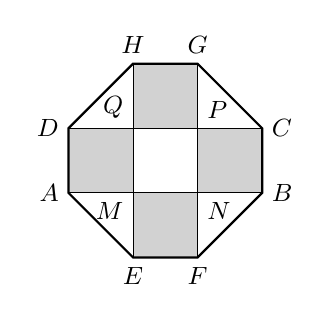
\begin{tikzpicture}[scale=0.82, every node/.style={font=\small}]
  \fill[gray!35] (-1.5,-0.5) rectangle (1.5,0.5);
  \fill[gray!35] (-0.5,-1.5) rectangle (0.5,1.5);
  % 中心正方形 MNPQ 原卷不涂阴影，照原卷留白：
  \fill[white] (-0.5,-0.5) rectangle (0.5,0.5);
  \draw[thick] (-1.5,0.5)--(-0.5,1.5)--(0.5,1.5)--(1.5,0.5)--(1.5,-0.5)--(0.5,-1.5)--(-0.5,-1.5)--(-1.5,-0.5)--cycle;
  \draw (-1.5,-0.5) rectangle (1.5,0.5);
  \draw (-0.5,-1.5) rectangle (0.5,1.5);
  \node[left] at (-1.5,0.5) {$D$};
  \node[left] at (-1.5,-0.5) {$A$};
  \node[right] at (1.5,0.5) {$C$};
  \node[right] at (1.5,-0.5) {$B$};
  \node[above] at (-0.5,1.5) {$H$};
  \node[above] at (0.5,1.5) {$G$};
  \node[below] at (-0.5,-1.5) {$E$};
  \node[below] at (0.5,-1.5) {$F$};
  \node[below left] at (-0.5,-0.5) {$M$};
  \node[below right] at (0.5,-0.5) {$N$};
  \node[above right] at (0.5,0.5) {$P$};
  \node[above left] at (-0.5,0.5) {$Q$};
\end{tikzpicture}
\end{center}

\begin{enumerate}[label=(\arabic*)]
\item 设 $DQ$ 长为 $y$（单位：m），用 $x$ 表示 $y$，并求出 $x$ 的取值范围；
\item $AD$ 取何值时可使总造价最低，并求出最低造价.
\end{enumerate}

\ifanswer
\solbegin
\stepm{(1)}{设 $AD=x\text{m}$（$x>0$），$DQ=y\text{m}$（$y>0$），}
\step{因为十字形区域总面积为 $200\text{m}^2$，所以 $4xy+x^2=200$，}
\step{解得 $y=\dfrac{200-x^2}{4x}=\dfrac{50}{x}-\dfrac{x}{4}$，}
\step{因为 $x>0$，$y>0$，所以 $y=\dfrac{200-x^2}{4x}>0$，解得 $0<x<10\sqrt2$，}
\step{所以 $y=\dfrac{50}{x}-\dfrac{x}{4}$，$0<x<10\sqrt2$；}
\stepm{(2)}{中心正方形 $MNPQ$ 区域，造价为 $2100$ 元$/\text{m}^2$，}
\step{中心正方形 $MNPQ$ 面积为 $S_1=x^2$，造价为 $W_1=2100\times S_1=2100x^2$；}
\step{周围四个矩形区域（图中阴影部分）铺设透水地砖，造价为 $105$ 元$/\text{m}^2$，}
\step{四个矩形的总面积为 $S_2=4xy=4x\left(\dfrac{50}{x}-\dfrac{x}{4}\right)=200-x^2$，}
\step{造价为 $W_2=105\times S_2=105(200-x^2)=21000-105x^2$；}
\step{四个三角形区域种植耐旱固碳植物，助力碳中和，造价为 $40$ 元$/\text{m}^2$，}
\step{四个三角形的总面积为 $S_3=4\times\dfrac12y^2=2\left(\dfrac{50}{x}-\dfrac{x}{4}\right)^2
=\dfrac{5000}{x^2}-50+\dfrac{x^2}{8}$，}
\step{造价为 $W_3=40\times S_3=40\left(\dfrac{5000}{x^2}-50+\dfrac{x^2}{8}\right)
=\dfrac{200000}{x^2}-2000+5x^2$；}
\step{设总造价为 $W$（单位：元），}
\step{则总造价为 $W=W_1+W_2+W_3$}
\step{$=2100x^2+21000-105x^2+\dfrac{200000}{x^2}-2000+5x^2$}
\step{$=2000x^2+\dfrac{200000}{x^2}+19000$，}
\step{又 $2000x^2+\dfrac{200000}{x^2}\geqslant2\sqrt{2000x^2\times\dfrac{200000}{x^2}}=2\times20000=40000$，}
\step{当且仅当 $2000x^2=\dfrac{200000}{x^2}$，即 $x=\sqrt{10}$（在 $x$ 的范围内）时取等号，}
\step{所以 $W=2000x^2+\dfrac{200000}{x^2}+19000\geqslant59000$，当 $x=\sqrt{10}$ 时取等号，}
\step{故当 $AD$ 的长为 $\sqrt{10}$ 时，总造价最低，为 $59000$ 元.}
\solend

\fi

\ansspace[8]

\item 对于实数 $a$、$b$、$c$，若 $|a-c|<|b-c|$，则称 $a$ 比 $b$ 更接近于 $c$. 现已知 $p$、$q$ 都是正有理数.

\begin{enumerate}[label=(\arabic*)]
\item 证明：$\sqrt3$ 必在 $\dfrac pq$ 和 $\dfrac{p+3q}{p+q}$ 之间；
\item 试问 $\dfrac pq$ 和 $\dfrac{p+3q}{p+q}$ 这两个数，哪一个更接近于 $\sqrt3$？说明你的理由；
\item 请你再写出一个有理数，使得它的值比 $\dfrac pq$ 和 $\dfrac{p+3q}{p+q}$ 的值更接近于 $\sqrt3$，并说明你的理由.
\end{enumerate}

\ifanswer
\solbegin
\stepm{(1)}{设 $a=\dfrac pq$（$a$ 为正有理数），则需证 $\sqrt3$ 在 $a$ 和 $\dfrac{a+3}{a+1}$（即 $\dfrac{p+3q}{p+q}$）之间.}
\step{当 $a>\sqrt3$ 时，计算 $a-\dfrac{a+3}{a+1}$ 得 $a-\dfrac{a+3}{a+1}=\dfrac{a(a+1)-(a+3)}{a+1}=\dfrac{a^2-3}{a+1}$，}
\step{$a>\sqrt3$，则 $a^2-3>0$，故 $a>\dfrac{a+3}{a+1}$；}
\step{再计算 $\dfrac{a+3}{a+1}-\sqrt3$ 得 $\dfrac{a+3}{a+1}-\sqrt3=\dfrac{(1-\sqrt3)(a-\sqrt3)}{a+1}$，}
\step{$1-\sqrt3<0$，$a-\sqrt3>0$，$a+1>0$，}
\step{故 $\dfrac{a+3}{a+1}-\sqrt3<0$，即 $\dfrac{a+3}{a+1}<\sqrt3$，从而 $\dfrac{a+3}{a+1}<\sqrt3<a$；}
\step{当 $a<\sqrt3$ 时，同理可得 $a<\dfrac{a+3}{a+1}$ 且 $\dfrac{a+3}{a+1}>\sqrt3$，即 $a<\sqrt3<\dfrac{a+3}{a+1}$，}
\step{综上，$\sqrt3$ 必在 $\dfrac pq$ 和 $\dfrac{p+3q}{p+q}$ 之间；}
\stepm{(2)}{设 $a=\dfrac pq$，$b=\dfrac{p+3q}{p+q}=\dfrac{a+3}{a+1}$，比较 $|a-\sqrt3|$ 与 $|b-\sqrt3|$，}
\step{由（1）得 $(a-\sqrt3)(b-\sqrt3)<0$，}
\step{$\dfrac{|b-\sqrt3|}{|a-\sqrt3|}
=\left|\dfrac{b-\sqrt3}{a-\sqrt3}\right|
=\dfrac{\left|\dfrac{(1-\sqrt3)(a-\sqrt3)}{a+1}\right|}{|a-\sqrt3|}
=\dfrac{\sqrt3-1}{a+1}$，}
\step{$a>0$，$a+1>1$，$\sqrt3-1<1$，故 $\dfrac{\sqrt3-1}{a+1}<1$，即 $|b-\sqrt3|<|a-\sqrt3|$，}
\step{即 $\dfrac{p+3q}{p+q}$ 比 $\dfrac pq$ 更接近于 $\sqrt3$；}
\stepm{(3)}{$\dfrac{2p+3q}{p+2q}$，理由：}
\step{设 $b=\dfrac{p+3q}{p+q}$，新数 $c=\dfrac{b+3}{b+1}=\dfrac{2p+3q}{p+2q}$，}
\step{由（1）得 $(b-\sqrt3)(c-\sqrt3)<0$，}
\step{$c-\sqrt3=\dfrac{b+3}{b+1}-\sqrt3=\dfrac{(1-\sqrt3)(b-\sqrt3)}{b+1}$，}
\step{则 $\dfrac{|c-\sqrt3|}{|b-\sqrt3|}
=\left|\dfrac{c-\sqrt3}{b-\sqrt3}\right|
=\dfrac{\left|\dfrac{(1-\sqrt3)(b-\sqrt3)}{b+1}\right|}{|b-\sqrt3|}
=\dfrac{\sqrt3-1}{b+1}$，}
\step{$b>0$，$b+1>1$，$0<\sqrt3-1<1$，故 $\dfrac{\sqrt3-1}{b+1}<1$，即 $|c-\sqrt3|<|b-\sqrt3|$，}
\step{即 $\dfrac{2p+3q}{p+2q}$ 比 $\dfrac{p+3q}{p+q}$ 更接近于 $\sqrt3$，故 $c$ 更接近 $\sqrt3$.}
\solend

\fi

\ansspace*[10]

\end{enumerate}

\end{document}
